\documentclass{book} 
\usepackage{graphicx} % Required for inserting images
\usepackage{mathrsfs}
\usepackage{amssymb}
\usepackage{amsmath}
\usepackage{indentfirst}
\usepackage{color}
\usepackage{hyperref}
\usepackage{xypic}
\usepackage{bbm}
\usepackage{dutchcal}
\hypersetup{hidelinks,
	colorlinks=true,
	allcolors=black,
	pdfstartview=Fit,
	breaklinks=true
}
\newcommand{\abs}[1]{\left\lvert #1 \right\rvert} 
\newcommand{\leftbracket}{[}
\newcommand{\rightbracket}{]}
\begin{document}
\tableofcontents
\part{Set}
\chapter{product}
\section{direct sum}
$\bigoplus $ is defined to be the direct product but with only finite non-zero elements.$$\bigoplus\limits_{i\in I}V_i\{(x_i)_{i\in I}\in \prod\limits_{i\in I}V_i\mid \exists J\subseteq I,I\setminus J \text{ is finite that } \forall j\in J,x_j=0\}$$
\chapter{Ring}
\section{morphism}
    \subsection*{Def}
    \indent Let A and B be unitary rings .We call morphism of unitary rings from A to B .only mapping $A\rightarrow B$is a morphism of group from (A,+) to (B,+),and a morphism of monoid from $(A,\cdot)\ to\ (B,\cdot)$
    \subsection*{Properties}
    \begin{itemize}
        \item Let R be a unitary ting. There is a unique morphism from $\mathbb{Z}\ to\ R$
        \item 
    \end{itemize}
\subsection*{algebra}

we call k-algebra any pair(R,f),when R is a unitary ring ,and $f:k\rightarrow R$ is a morphism of unitary rings such that $\forall (b,x)\in k\times R,f(b)x=xf(b)$

Example:    For any unitary ring R,the unique morphism of unitary rings $\mathbb{Z}\rightarrow R$ define a structure of $\mathbb{Z}-algebra$ on R (extra: $\mathbb{Z}$ is commutative despite R isn't guaranteed)

Notation: Let k be a commutative unitary ring ,(A,f) be a k-algebra. If there is no ambiguity on f,for any$ (\lambda,a )\in k\times A$,we denote $f(\lambda)a\ as\ \lambda a$
\subsection*{Formal power series}
reminder: $n\in\mathbb{N}$ is possible infinite ,so $\sum\limits_{n\in \mathbb{N}}$ couldn't be executed directly.
Def:

(extended polynomial actually)
Let k be a commutative unitary ring.
Def : Let T be a formal symbol.We denote $k^\mathbb{N}$ as $k\mathbb{[}T\mathbf{]}$ If $(a_n)_{n\in\mathbb{N}}$ is an element of $k^\mathbb{N}$,when we denote $k^\mathbb{N}$ as k[T] this element is denote as $\sum_{n\in\mathbb{N}}a_nT^n$ Such element is called a formal power series over k and $a_n$ is called the Coefficient of $T^n$ of this formal power series
Notation: \begin{itemize}
    \item omit terms with coefficient O
    \item write T' as T
    \item omit Coefficient those are 1;
    \item omit $T^0$
\end{itemize}
Example $1T^0+2T^1+1T^2+0T^3+...+0T^n+...$ is written as $1+2T+T^2$

Def Remind that k[T]=$\{\sum_{n\in\mathbb{N}}a_nT^n\mid (a_n)_{n\in\mathbb{N}}\in k^\mathbb{N} \}$,define two composition laws on k[T]\\
$\forall F(T)=a_0+a_+1T+...\quad G(T)=b_0+...$\\
let $F+G=(a_0+b_0)+...$\\
$FG=\sum\limits_{n\in\mathbb{N}}\sum\limits_{i+j=n}(a_ib_j)T^n$\\
Properties:\begin{itemize}
\item $(k[T],+,\cdot)$form a commutative unitary ring.
\item $k\rightarrow k[T]\quad \lambda\mapsto\lambda T$ is a morphism 
\item $(FG)H=\left(\sum_{n\in\mathbb{N}}^{}\sum\limits_{i+j=n}(a_ib_j)T^n\right)(\sum\limits_{n\in\mathbb{N}}c_nT^n)=\sum\limits_{n\in\mathbb{N}}\left(\sum\limits_{p,q,l=n}a_pb_qc_l\right)T^n$\\is a trick applied on integral
\end{itemize}
Derivative:

let $F(T)\in k[T]$\\
\indent We denote by $F'(T)\ or\ \mathcal{D}(F(T))$ the formal power series\\
\indent$\mathcal{D}(F)=\sum\limits_{n\in\mathbb{N}}(n+1)a_{n+1}T^n$\\
Properties:\begin{itemize}
    \item $\mathcal{D}(k[T],+)\rightarrow(k[T],+)$ is a morphism of groups
    \item $\mathcal{D}(FG)=F'G+FG'$
\end{itemize}
exp

We denote $exp(T)\in k[T]$ as $\sum\limits_{n\in\mathbb{N}}{1\over n!}T^n$,which fulfil the differential equation $\mathcal{D}(exp(T))=exp(T)$(interesting)\\
Cauchy sequence: $(F_i(T))_{i\in\mathbb{N}}$ be a sequence of elements in k[T],and $F(T)\in k[T]$We say that $(F_i(T))_{i\in \mathbb{N}}$ is a Cauchy sequence if $\forall l \in \mathbb{N}$,there exists $N(l)\in \mathbb{N}$ such that $\forall(i,j)\in\mathbb{N}^2_{\geq N(l)},ord(F_i(T)-F_j(T))\geq l$
\part{Sequences}
\chapter{Supremum and infimum}
Def:

Let $(X,\le)$ be a partially ordered set A and Y be subsets of X,such that $A\subseteq Y$
\begin{itemize}
    \item If the set $\{y\in Y\mid \forall a \in A,a\leq Y\}$has a least element then we say that A has a Supremum in Y with respect to $\leq$ denoted by $sup_{(y,\leq)}A$ this least element and called it the Supremum of A in Y(this respect to $\leq$)
    \item If the set $\{y\in Y\mid\forall a\in A,y\leq a\}$ has a greatest element, we say that A has n infimum in Y with respect to $\leq$ .We denote by $inf_{(y,\leq)}A$ this greatest element and call it the infimum of A in Y 
    \item Observation: $inf_{(Y,\leq)}A=sup_{(Y,\geq)}A$
\end{itemize}
Notation:

Let $(X,\leq)$ be a partially ordered set,I be a set.
\begin{itemize}
    \item If f is a function from I to X sup f denotes the supremum of f(I) is X.$\inf f $takes the same
    \item If $(x_i)_{i\in I} is \ a\ family\ of\ element\ in\ X,then\ \sup \limits_{i\in I}x_i\ denotes\ \sup\{x_i\mid i\in I\} (in X)$
\end{itemize}

If moreover $\mathbb{P}(\cdot)$ denotes a statement depending on a parameter in I then $\sup\limits_{i\in I,\mathbb{P}(i)}x_i$ denotes $\sup\{x_i\mid i\in I,\mathbb{P}(i)\ holds\}$\\
Example:

Let $A={x\in R\mid 0\leq x<1}\subseteq \mathbb{R}$ We equip $\mathbb{R}$ with the usual order relation.$$\{y\in \mathbb{R}\mid \forall x\in A,x\leq y\}=\{y\in\mathbb{R}\mid y\geq 1\}$$
So $\sup A=1$
$$\{y\in \mathbb{R}\mid \forall x\in A,y\leq x\}=\{y\in\mathbb{R}\mid y\geq 0\}$$
Hence $\inf A=0$\\
Example: 
For $n\in \mathbb{N}$,let $x_n=(-1)^n\in R$ $$\sup\limits_{n\in \mathbb{N}}\inf\limits_{k\in \mathbb{N},k\geq n}x_k=-1$$
Proposition:

Let $(X,\leq)$ be a partially ordered set,A,Y,Z be subset of X,such that $A\subseteq Z\subseteq Y$
\begin{itemize}
    \item If max A exists,then is is also equal to $\sup_{(y,\leq)}A$
    \item If $\sup_{(y,\leq)}A$ exists and belongs to Z, then it is equal to $\sup A$
\end{itemize}

$\inf$ takes the same
Prop.

Let $X,\leq$ be a partially ordered set ,A,B,Y be subsets of X such that $A\subseteq B\subseteq Y$
\begin{itemize}
    \item If $\sup_{(y,\leq)}A$ and $\sup_{(y,\leq)}B$ exists,then $\sup_{(y,\leq)}A \leq \sup_{(y,\leq)}B$
    \item If $\inf_{(y,\leq)}A$ and $\inf_{(y,\leq)}B$ exists,then $\inf_{(y,\leq)}A \geq \inf_{(y,\leq)}B$
\end{itemize}
Prop.

Let $(X,\leq)$be a partially ordered set ,I be a set and $f,g:I\rightarrow X$ be mappings such that $\forall t\in I,f(t)\leq g(t)$
\begin{itemize}
    \item If $\inf f$ and $\inf g$ exists,then $\inf f\leq \inf g$ 
    \item If $\sup f$ and $\sup g$ exists,then $\sup f\leq \sup g$ 
\end{itemize}
\chapter{Interval}
We fix a totally ordered set $(X,\leq)$\\
Notation:

If $(a,b)\in X\times X $ such that $a\leq b $,[a,b] denotes $\{x\in X\mid a\leq x\leq b\}$\\
Def:

Let $I\subseteq X $. If $\forall(x,y)\in I\times I$ with $x\leq y$,one has $[x,y]\subseteq I$ then we say that I is a interval in X\\
Example:

Let $(a,b)\in X\times X$, such that $a\leq b$ Then the following sets are intervals
\begin{itemize}
    \item $]a,b[:=\{x\in X\mid a,x,b\}$
    \item $[a,b[:=\{x\in X\mid a,x,b\}$
    \item $]a,b]:=\{x\in X\mid a,x,b\}$
\end{itemize}
Prop. 

Let $\Lambda$ be a non-empty set and $(I_\lambda)_{\lambda\in \Lambda}$ be a family of intervals in X.
\begin{itemize}
    \item $\bigcap\limits_{\lambda\in\Lambda}I_\lambda$ is a interval in X
    \item If $\bigcap\limits_{\lambda\in\Lambda}I_\lambda\not=\varnothing $,$\bigcup\limits_{\lambda\in\Lambda}I_\lambda$ is a interval in X
\end{itemize}
We check that $[a,b]\subseteq I_\lambda\cup I_]\mu$
\begin{itemize}
    \item If $b\leq x$\quad $[a,b]\subseteq[a,x]\subseteq I_\lambda$ because $\{a,x\}\subseteq I_\lambda$
    \item If $x\leq a$\quad $[a,b]\subseteq[x,b]\subseteq I_\mu $ because $\{b,x\}\subseteq I_\mu$
    \item If a $<$ x $<$ b then $[a,b]=[a,x]\cup[x,b]\subseteq I_\lambda\cup I_\mu$
\end{itemize}
Def:

Let $(X,\leq)$ be a totally ordered set .I be a non-empty interval of X. If $\sup I$ exists in X, we call $\sup I$ the right endpoint; inf takes the similar way.\\
Prop.

Let I be an interval in X.
\begin{itemize}
    \item Suppose that $b=\sup I$exists. $\forall x\in I,[x,b[\subseteq I$
    \item Suppose that $a=\inf I$exists. $\forall x\in I,]a,x]\subseteq I$
\end{itemize}
Prop.

Let I be an interval in X. Suppose that I has supremum b and an infimum a in X.Then I is equal to one of the following sets $[a,b]\ \ [a,b[\ \ ]a,b]\ \ ]a,b[$\\
Def 

let $(X,\leq)$ be a totally ordered set .If $\forall (x,z)\in X\times X$,such that $x<z\quad \exists y\in X$ such that $x<y<z$,than we say that $(X,\leq)$ is thick\\
Prop. 

Let $(X,\leq)$ be a thick totally ordered set. $(a,b)\in X\times X,a<b$ If I is one of the following intervals $[a,b];[a,b[;]a,b];]a,b[$ Then $\inf I=a\quad \sup I=b$ (for it's thick empty set is impossible)\\
Proof:

Since X is thick,there exists $x_0\in]a,b[$ By definition,b is an upper bound of I. If b is not the supremum of I,there exists an upper bound M of I such that M<b. Since X is thick ,there is $M'\in X$ such that $x_0\leq M,M'<b$ Since $[x,b[\subseteq]a,b[\in I$ Hence M and M' belong to I,which conflicts with the uniqueness of supremum.
\chapter{Enhanced real line}
Def:

Let $+\infty$ and $-infty$ be two symbols that are different and don not belong to $\mathbb{R}$ We extend the usual total order $\leq\ on\ \mathbb{R}\ to\ \mathbb{R}\cup\{-\infty,+\infty\}$ such that $$\forall x\in \mathbb{R} ,-\infty<x<+\infty$$ 
\indent Thus $\mathbb{R} \cup\{-\infty,+\infty\}$ become a totally ordered set, and $\mathbb{R} =]-\infty,+\infty[$  Obviously,this is a thick totally ordered set.\\
We define:
\begin{itemize}
    \item $\forall x\in ]-\infty,+\infty]\quad x+(+\infty):=+\infty \quad (+\infty)+x:=+\infty$
    \item $\forall x\in [-\infty,+\infty[\quad x+(-\infty):=-\infty\quad (-\infty)+x=-\infty$
    \item $\forall x\in ]0,+\infty]\quad x(+\infty)=(+\infty)x=+\infty\quad x(-\infty)=(-\infty)x=-\infty$
    \item $\forall x\in [-\infty,0[\quad x(+\infty)=(+\infty)x=-\infty\quad x(-\infty)=(-\infty)x=+\infty$
    \item $-(+\infty)=-\infty\quad -(-\infty)=+\infty\quad (\infty)^{-1}=0$
    \item $(+\infty)+(-\infty)\quad (-\infty)+(+\infty)\quad (+\infty)0\quad 0(+\infty)\quad(-\infty)0\quad 0(-\infty)$ \\\textcolor{red}{ARE NOT DEFINED}
\end{itemize}
Def 

Let $(X,\leq)$ be a partially ordered set. If for any subset A of X,A has a supremum and an infimum in X, then we say the X is order complete\\
Example

Let $\Omega$ be a set $(\mathscr{P}(\Omega),\subseteq)$is order complete If $\mathscr{F}$is a subset of $\mathscr{P}(\Omega),\sup\mathscr{F}=\bigcup\limits_{A\in \mathscr{F}}A$

Interesting tip: $\inf \varnothing =\Omega\quad \sup \varnothing=\varnothing$\\
$\mathcal{AXION}:$\\\indent$(\mathbb{R}\cup\{-\infty,+\infty\},\leq)$ is order complete \\\indent In $\mathbb{R}\cup\{-\infty,+\infty\}\quad \sup\varnothing=-\infty\quad\inf\varnothing=+\infty$\\
Notation:
\begin{itemize}
    \item For any $A\subseteq \mathbb{R} \cup{-\infty,+\infty}\ and\ c\in \mathbb{R} $ We denote by $A+c$ the set $\{a+c\mid a\in A\}$
    \item If $\lambda\in\mathbb{R} \backslash\{0\},\lambda A$ denotes $\{\lambda a\mid a\in A\}$
    \item -A denotes (-1)A
\end{itemize}
Prop.

For any $A\subseteq\mathbb{R} \cup\{-\infty,+\infty\},\sup(-A)=-\inf A,\inf (-A)+-\sup A$
Def 

We denote by $(R,\leq)$ a field $\mathbb{R} $ equipped with a total order $\leq$, which satisfies the following condition:
\begin{itemize}
    \item $\forall (a,b)\in \mathbb{R} \times \mathbb{R} $ such that $a<b$ ,one has $\forall c\in \mathbb{R} ,a+c<b+c$
    \item $\forall(a,b)\in\mathbb{R}_{>0}\times\mathbb{R}_{>0},ab>0$
    \item $\forall A\subseteq \mathbb{R} $,if A hsa an upper bound in$\mathbb{R}$ ,then it has a supremum in$\mathbb{R} $
\end{itemize}
Prop.

Let $A\subseteq[-\infty,+\infty]$
\begin{itemize}
    \item $\forall c\in \mathbb{R} \quad \sup(A+c)=(\sup A)+c$
    \item $\forall \lambda\in \mathbb{R}_{\geq0}\quad \sup(\lambda A)=\lambda\sup(A)$
    \item $\forall\lambda\in \mathbb{R} _{\leq0}\quad sup(\lambda A)=\lambda\inf(A)$
\end{itemize}

\indent $\inf$ takes the same\\
Theorem:

Let I and J be non-empty sets\\
\indent$f:I\rightarrow[-\infty,+\infty],g:J\rightarrow[-\infty,+\infty]$\\
\indent$a=\sup\limits_{x\in I}f(x)\quad b=\sup\limits_{y\in J}g(y)\quad c=\sup\limits_{(x,y)\in I\times J,\{f(x),g(y)\}\not=\{+\infty,-\infty\}}(f(x)+g(y))$ \\
\indent If $\{a,b\}\not=\{+\infty,-\infty\}$then $c=a+b$\\
\indent $\inf$ takes the same if $(-\infty)+(+\infty)$ doesn't happen\\
Corollary:

Let I be a non-empty set,$f:I\rightarrow[-\infty,+\infty],g:J\rightarrow[-\infty,+\infty]$\\
Then $\sup\limits_{x\in I,\{f(x),g(y)\}\not=\{+\infty,-\infty\}}(f(x)+g(x))\leq(\sup\limits_{x\in I}f(x))(\sup\limits_{x\in I}g(x))$\\
\indent $\inf$ takes the similar($\leq\rightarrow\geq$) (provided when the sum are defined)
\chapter{Vector space}
In this section:\\
\indent K denotes a unitary ring.\\
\indent Let 0 be zero element of K\\
\indent 1 be the unity of K
\section{K-module}
\subsection{Def}

Let $(V,+)$ be a commutative group.We call left/right K-module structure:\\
\indent any mapping $\Phi$:$K\times V\rightarrow V$
\begin{itemize}
    \item $\forall(a,b)\in K\times K,\forall x\in V\quad \Phi(ab,x)=\Phi(a,\Phi(b,x))/\Phi(b,\Phi(a,x))$
    \item $\forall (a,b)\in K\times K,\forall x\in V,\Phi(a+b,x)=\Phi(a,x)+\Phi(b,x)$
    \item $\forall a\in K,\forall(x,y)\in V\times V,\Phi(a,x+y)=\Phi(a,x)+\Phi(a,y)$
    \item $\forall x\in V,\Phi(1,x)=x$
\end{itemize}
A commutative group (V,+) equipped with a left/right K-module structure is called a left/right K-module.
\subsection{Remark}\quad Let $K^{op}$ be the set K equipped with the following composition laws:
\begin{itemize}
    \item $K\times K\rightarrow K$
    \item $(a,b)\mapsto a+b$
    \item $K\times K\rightarrow K$
    \item $(a,b)\mapsto ba$
\end{itemize}
Then $K^{op}$ forms a unitary ring\\
Any left $K^{op}-module$ is a right K-module\\
Any right $K^{op}-module$ is a left K-module\\
$(K^{op})^{op}=K$
\subsection{Notation}

When we talk about a left/right K-module $(V,+)$,we often write its left K-module structure as $K\times V\rightarrow V\quad (a,x)\mapsto ax$\\
\indent The axioms become:\begin{align*}
    &\forall(a,b)\in K\times K,\forall x\in V\quad (ab)x=a(bx)/b(ax)\\
    &\forall(a,b)\in K\times K,\forall x\in V\quad (a+b)x=ax+bx\\
    &\forall a\in K,\forall(x,y)\in V\times V\quad a(x+y)=ax+ay\\
    &\forall x\in V\quad 1x=x
\end{align*}
\subsection{K-vector space}

If K is commutative,then $K^{op}=K$,so left K-module and right K-module structure are the same .We simply call them K-module structure. A commutative group equipped with a K-module structure is called a K-module.If K is a field,a K-module is also called a K-vector space

Let $\Phi:K\times V\rightarrow V$ be a left or right K-module structure$$\forall x\in V,\Phi(\cdot,x):K\rightarrow V\quad(a\in K)\mapsto\Phi(a,x)$$\indent is a morphism of addition groups.Hence $\Phi(0,x)=0,\Phi(-a,x)=-\Phi(a,x)$\\
$\forall a\in K,\Phi(a,\cdot):V\rightarrow V$ is a morphism of groups.Hence $\Phi(a,0)=0,\Phi(a,-x)=-\Phi(a,x)(\cdot \ is\ a\ var)$
\subsection{Association:}
$\forall x\in K$
\begin{align*}
    (f(f+g)+h)(x)=(f+g)(x)+h(x)=f(x)+g(x)+h(x)\\
    (f+(g+h))(x)=f(x)+((g+h)(x))=f(x)+g(x)+h(x)
\end{align*} 

Let $0:I\rightarrow K:x\mapsto0 \quad \forall f\in K^I\quad f+0=f$\\
Let $-f: f+(-f)=0$\\
The mapping $K\times K^I\rightarrow K^I:(a,f)\mapsto af\quad (af)(x)=af(x)$ is a left K-module structure\\
The mapping $K\times K^I\rightarrow K^I:(a\in I)\mapsto ((x\in I)\mapsto f(x)a)\quad (af)(x)=af(x)$ is a right K-module structure
\subsection{Remark:}

We can also write an element $\mu\ of\ K^I$ is the form of a family $(\mu_i)_{i\in I}$ of elements in K ($\mu_i$is the image of $i\in I\ by\ \mu$)\\
Then \begin{align*}
    &(\mu_i)_{i\in I}+(\nu_i)_{i\in I}:=(\mu_i+\nu_i)_{i\in I}\\
    &a(\mu_i)_{i\in I}:=(a\mu_i)_{i\in I}\\
    &(\mu_i)_{i\in I}a=(\mu_ia)_{i\in I}
\end{align*}
\section{sub K-module}
\subsection{Def}

Let V be a left/right K-module.If W is a subgroup of V. Such that $\forall a\in K,\forall x\in W\quad ax/xa\in W$, then we say that W is left/right sub-K-module of V.
\subsection{Example}

Let I be a set .Let $K^{\bigoplus I}$ be the subset of $K^I$ composed of mappings $f:I\rightarrow K$ such that $I_f=\{x\in I\mid f(x)\not=0\}$ is finite. It is a left and right sub-K-module of $K^I$\\
\indent In fact,$\forall (f,g)\in K^{\bigoplus I}\times K^I\quad I_{f-g}={x\in I\mid f(x)-g(x)\not=0}\subseteq I_f\cup I_g$\\
\indent Hence $f-g\in K^{\bigoplus I}$ So $K^{\bigoplus I}$ is a subgroup of $K^I$\\
\indent $\forall a\in K,\forall f\in K^{\bigoplus I}\quad I_{af}\subseteq I_f,I_{(x\mapsto f(x)a)}\subseteq I_f$
\section{morphism of K-modules}
\subsection{Def}

Let V and W be left K-module, A morphism of groups $\phi:V\rightarrow W$ is called a morphism of left K-modules if $\forall(a,x)\in K\times V,\phi(ax)=a\phi(x)$
\subsection{K-linear mapping}
\indent If K is commutative, a morphism of K-modules is also called a K-linear mapping. We denote by $\hom_{K-Mod}(V,W)$ the set of all morphism of left-K-module from V to W.This is a subgroup of $W^V$
\subsection{Theorem}

Let V be a left K-module. Let I be a set.\\
The mapping $\hom_{K-Mod}(K^{\bigoplus I},V)\rightarrow V^I:\ \phi\rightarrow (\phi(e_i))_{i\in I}$ is a bijection where $e_i:I\rightarrow K:j\mapsto\left\{\begin{aligned}
    1\quad j=i\\
    0\quad j\not=i
\end{aligned} \right.$
\subsection{Remark:column}

In the case where $I={1,2,3,...,n}\ V^I$ is denoted as $V^n,K^I$ is denoted as $K^n$\\
For any $(x_1,...,x_n)\in V^n$,by the theorem, there exists a unique morphism of left K-modules $\phi:K^n\rightarrow V$ such that $\forall i\in{1,...,n}\phi(e_i)=x_i$\\
We write this $\phi$ as a column$\begin{pmatrix}
    x_1\\
    ...\\
    x_n
\end{pmatrix}$It sends $(a_1,...,a_n)\in K^n$ to $a_1x_1+...+a_nx_n$
\section{kernel}
\subsection{Prop}

Let G and H be groups and $f:G\rightarrow H$ be a morphism of groups\begin{itemize}
    \item $I_m(f)\subseteq H $ is a subgroup of H
    \item $\ker(f)=\{x\in G\mid f(x)=e_H\}$
    \item $f$ is injection iff $\ker(f)=\{e_G\}$
\end{itemize}
\subsection{Def}

$\ker(f)$ is called the kernel of $f$
\subsection{Theorem}
$f$ is injection iff $\ker(f)=\{e_G\}$
\subsection*{Proof}
Let $e_G$ and $e_H$ be neutral element of G and H respectively
\begin{itemize}
    \item [(1)]Let x and y be element of G\\$f(x)f(y)^{-1}=f(x)f(y)^{-1}=f(xy^{-1})\in Im(f).$ So $Im(f)$ is a subgroup of H
    \item [(2)]Let x and y be element of $\ker(f)$ One has $f(xy^{-1})=f(x)f(y)^{-1}=e_H\quad e_H^{-1}=e_H.$ So $xy^{-1}\in\ker(f)$ So $\ker(f)$ is a subgroup of G
    \item [(3)]Suppose that f is injection.\\ Since $f(E_G)=e_H$ one has $\ker(f)=f^{-1}(\{e_H\})=\{e_G\}$ Suppose that $\ker(f)=\{e_G\}$ If $f(x)=f(y)$then $f(xy^{-1})=f(x)f(y)^{-1}=e_H$\\Hence $xy^{-1}=e_G\ \Rightarrow\ x=y$
\end{itemize}
\subsection{Def}

Let (V,+) be a commutative group, I be a set. We define a composition law + on $V^I$ as follows$$(x_i)_{i\in I}+(y_i)_{i\in I}\ :=(x_i+y_i)_{i\in I}$$
Then $V^I$ forms a commutative group
\subsection{Remark}

Let E and F be left K-modules\\$\hom_{K=Mod}(E,F):=\{\text{morphisms of left K-modules from E to F}\}\subseteq F^E$ is a subgroup of $F^E$\\
In fact f and g are elements of $\hom_{K-Mod}(E,F)$, then $f-g$ is also a morphism of left K-module\\$(f-g)(x+y)=f(x+y)-g(x+y)=(f(x)+f(y))-(g(x)+g(y))=(f(x)-g(x))+(f(y)-g(y))=(f-g)(x)+(f-y)(x)$
\subsection{Theorem}

Let V be a left K-module,I be a set The mapping $\hom_{K-Mod}(K^{\bigoplus I},V)\rightarrow V^I\ :\ \phi\mapsto(\phi(e_i))_i\in I$ is an isomorphism of groups, where $e_i:I\rightarrow K:j\mapsto\left\{\begin{aligned}
    1\quad j=i\\
    0\quad j\not=i
\end{aligned} \right.$
\subsection{Proof:}
One has $(\phi+\psi)(e_i)=\phi(e_I)+\psi(e_i)$\\
$\forall(\phi,psi)\in \hom_{K-Mod}(K^{\bigoplus I},V)^2$\\
Hence $\Psi(\phi,\psi)=(\phi(e_i)+\psi(e_i))_{i\in I}=\Psi(\phi)+\Psi(\psi)$\\
So $\Psi$ is a morphism of groups
\begin{itemize}
    \item [injectivity] Let $\phi\in \hom_{K-Mod}(K^{\bigoplus I},V)$ Such that $\forall i\in I(\forall \phi\in\ker(\Psi))\quad\phi(e_i)=0$\\Let $a =(a_i)_{i\in I}\in K^{\bigoplus I}$ One has $a=\sum\limits_{i\in I}a_ie_i$ \\ If fact,$\forall j\in I,a_j=\sum\limits_{i\in I,a_i\not=0}a_ie_i(j)$\\Thus $\phi(a)=\sum\limits_{i\in I,a_i\not=0}a-I\phi(e_i)=0$\\Hence $\phi$ is the neutral element.
    \item [surjectivity] Let $x=(x_i)_{i\in I}\in V^I$ We define $\phi_x:K^{\bigoplus I}\rightarrow V$ such that $\forall a=(a_i)_{i\in I}\in K^{\bigoplus I},\phi_x(a)=\sum\limits_{i\in I,a_i\not=0}a_ix_i$\\This is a morphism of left K-modules\\$forall i\in I,\phi_x(e_i)=1x_i=x_i$  So $\Psi(\phi_x)=x$
\end{itemize}
{\color{blue}Suppose that K' is a unitary ring,and V is also equipped with a right K'-module structure, Then $\hom_{K-Mod}(K^{\bigoplus I},V)\subseteq V^{K^{\bigoplus I}}$ is a right sub-k'-module ,and $\Psi$ in the theorem is a right K'-module isomorphism}
\chapter{Monotone mappings}
\section{Def}

Let I and X be partially ordered sets,$f:I\rightarrow X$ be a mapping.
\begin{itemize}
    \item If $\forall(a,b)\in I\times I$ such that $a<b$. One has $f(a)\leq f(b)/f(a)<f(b)$,then we say that $f$ is increasing/strictly increasing. decreasing takes similar way.
    \item If $f$ is (strictly) increasing or decreasing, we say that $f$ is (strictly) monotone.
\end{itemize}
\section{Prop.}

Let  X,Y,Z be partially ordered sets.$f:X\rightarrow Y, g:Y\rightarrow Z$ be mappings
\begin{itemize}
    \item If $f$ and $g$ have the same monotonicity, then $g\circ f$ is increasing
    \item If $f$ and $g$ have different monotonicities, then $g\circ f$ is decreasing
\end{itemize}
strict monotonicities takes the same
\section{Def}

Let $f$ be a function from a partially ordered set I to another partially ordered set .If $f\mid_{Dom(f)}\rightarrow X$ is (strictly) increasing/decreasing then we say that $f$ is (strictly) increasing/decreasing
\section{Prop.}

Let I and X be partially ordered sets. $f$ be function from I to X.
\begin{itemize}
    \item If $f$ is increasing/decreasing and $f$ is injection, then $f$ is strictly increasing/decreasing
    \item Assume that I is totally ordered and $f$ is strictly monotone, then $f$ is injection
\end{itemize}
\section{Prop}

Let A be totally ordered set, B be a partially ordered set, $f$ be an injective function from A to B\\
If $f$ is increasing/decreasing ,then so is $f^{-1}$
\section{Def}
Let X and Y be partially ordered sets. $f:X\rightarrow Y$ be a bijection. If both $f$ and $f^{-1}$ are increasing ,then we say that $f$ is an isomorphism of partially ordered sets.\\
\indent(If X is totally, then a mapping $f:X\rightarrow Y$ is an isomorphism of partially ordered sets iff $f$ is a bijection and $f$ is increasing)
\section{Prop.}
Let I be a subset of $\mathbb{N} $ which is infinite. Then there is a unique increasing bijection $\lambda_I:\mathbb{N} \rightarrow I$
\section{Proof}
\subsection{bijection}
We construct $f:\mathbb{N} \rightarrow I$ by induction as follows.\\
Let $f(0)=\min I$ Suppose that $f(0),...,f(n)$ are constructed\\
then we take $f(n+1):=\min(I\backslash\{f(0),...,f(n)\})$\\
Since $I\backslash\{f(0),...,f(n-1)\}\supseteq I\backslash\{f(0),...,f(n)\}.$Therefore $f(n)\leq f(n+1)\\
Since f(n+1)\not\in\{f(0),...,f(n)\}$,we have $f(n)<f(n+1)$\\
Hence $f$ is strictly increasing and ths is injective\\
If $f$ is not surjective,then $I\backslash Im(f)$ has a element N. \\
Let $m=\min\{n\in\mathbb{N} \mid N\leq f(n)\}$.\\
Since $N\not\in Im(f),N<f(m)$.\\
So $m\not=0$.Hence $f(m-1)<N<f(m)=\min(I\backslash\{f(0),...,f(m-1)\})$ \\
By definition,$N\in I\backslash Im(f)\subseteq I\backslash \{f(0),...,f(m-1)\}$,\\Hence $f(m)\leq N$,causing contradiction.
\subsection{uniqueness}
exercise: Prove that $Id_\mathbb{N}$ is the only isomorphism of partially ordered sets from $\mathbb{N} $ to $\mathbb{N} $
\chapter{sequence and series}
Let $I\subseteq \mathbb{N}$ be a infinite subset
\section{Def} Let X be a set.We call sequence in X parametrized by I a mapping from I to X.
\section{Remark}
If K is a unitary ring and E is a left K-module then the set of sequence $E^I$ admits a left-K-module structure. If $x=(x_n)_{n\in I}$ is a sequence in E, we define a sequence $\sum(x):=(\sum\limits_{i\in I,i\leq n}x_i)_{n\in \mathbb{N}}$,called the series associated with the sequence x.
\section{Prop}
$\sum:E^I\rightarrow E^\mathbb{N}$ is a morphism of left-K-module
\section{proof}
Let $x=(x_i)_{i\in I}$ and $y=(y_i)_{i\in I}$ be elements of $E^I$\\
$\sum\limits_{i\in I,i\leq n}(x_i+y_i)=(\sum\limits_{i\in I,i\leq n}x_i)+(\sum\limits_{i\in I,i\leq n}y_i),\lambda\sum\limits_{i\in I,i\leq n}x_i=\sum\limits_{i\in I,i\leq n}\lambda x_i$
\section{Prop}
Let I be a totally ordered set . X be a partially ordered set,$f:I\rightarrow X$ be a mapping ,$J\in I$ Assume that J does not have any upper bound in I
\begin{itemize}
    \item If $f$ is increasing ,then $f(I)$ and $f(J)$ have the same upper bounds in X
    \item If $f$ is decreasing ,then $f(I)$ and $f(J)$ have the same lower bounds in X
\end{itemize}
\section{limit}
\subsection{Def}
Let $i\subseteq\mathbb{N}$ be a infinite subset.$\forall (x_i)_{n\in I}\in [-\infty,+\infty]^I$ where $[-\infty,+\infty]$ denotes $\mathbb{R}\cup\{-\infty,+\infty\}$,we define:
$$\limsup\limits_{n\in I,n\rightarrow +\infty}x_n:=\inf\limits_{n\in I}(\sup\limits_{i\in I,i\geq n}x_i)$$
$$\liminf\limits_{n\in I,n\rightarrow +\infty}x_n:=\sup\limits_{n\in I}(\inf\limits_{i\in I,i\geq n}x_i)$$
If $\limsup\limits_{n\in I,n\rightarrow +\infty}x_n=\liminf\limits_{n\in I,n\rightarrow +\infty}x_n=l$, we then say that $(x_n)_{n\in I}$ tends to $l$ and that $l$ is the limit of $(x_n)_{n\in I}$. If in addition $(x_n)_{n\in I}\in \mathbb{R}^I$ and $l\in \mathbb{R}$,we say that $(x_n)_{n\in I}$ converges to $l$
\subsection{Remark}
If $J\subseteq\mathbb{N}$ is an infinite subset, then: $$\limsup\limits_{n\in I,n\rightarrow +\infty}=\inf\limits_{n\in J}(\sup\limits_{i\in I,i\geq n}x_i)$$
$$\liminf\limits_{n\in I,n\rightarrow +\infty}x_n=\sup\limits_{n\in J}(\inf\limits_{i\in I,i\geq n}x_i)$$
Therefore ,if we change the values of finitely many terms in $(x_i)_{i\in I}$ the limit superior and the limit inferior do not change.\\
In fact, if we take $J=\mathbb{N}\backslash\{0,...,m\}$, then $\inf\limits_{n\in J}(...)$ and $\sup\limits_{n\in J}(...)$ only depends on the values of $x_i,i\in I,i\geq m$
\subsection{Prop}
$\forall (x_n)_{n\in I}\in [-\infty,+\infty]^I,\ \liminf\limits_{n\in I,n\rightarrow+\infty}x_n\leq\limsup\limits_{n\in I,n\rightarrow+\infty}x_n$
\subsection{Prop}
Let $(x_n)_{n\in I}\in[-\infty,+\infty]^I$
\begin{align*}
    &\forall c\in\mathbb{R} & \begin{aligned}
        \limsup\limits_{n\in I,n\rightarrow+\infty}(x_n+c)=(\limsup\limits_{n\in I,n\rightarrow+\infty}x_n)+c\\
        \liminf\limits_{n\in I,n\rightarrow+\infty}(x_n+c)=(\liminf\limits_{n\in I,n\rightarrow+\infty}x_n)+c
    \end{aligned}\\
    &\forall c\in \mathbb{R}_{>0} &\begin{aligned}
        \limsup\limits_{n\in I,n\rightarrow+\infty}(\lambda x_n)=\lambda\limsup\limits_{n\in I,n\rightarrow+\infty}x_n\\\liminf\limits_{n\in I,n\rightarrow+\infty}(\lambda x_n)=\lambda\liminf\limits_{n\in I,n\rightarrow+\infty}x_n
    \end{aligned}\\
    &\forall c\in \mathbb{R}_{<0} &\begin{aligned}
        \limsup\limits_{n\in I,n\rightarrow+\infty}(\lambda x_n)=\lambda\liminf\limits_{n\in I,n\rightarrow+\infty}x_n\\\liminf\limits_{n\in I,n\rightarrow+\infty}(\lambda x_n)=\lambda\limsup\limits_{n\in I,n\rightarrow+\infty}x_n
    \end{aligned}
\end{align*}
\subsection{Prop}
Let $(x_n)_{n\in I}$ be elements in $[-\infty,+\infty]^I$. Suppose that there exists $N_0\in \mathbb{N}$ such that $\forall n\in I,n\geq N_0$,one has $x_n\leq y_n$ Then $$\limsup\limits_{n\in I,n\rightarrow+\infty}(x_n)\leq\limsup\limits_{n\in I,n\rightarrow+\infty}y_n$$ ,$$\liminf\limits_{n\in I,n\rightarrow+\infty}(x_n)\geq\liminf\limits_{n\in I,n\rightarrow+\infty}y_n$$
\subsection{Theorem}
Let $(x_n)_{n\in I},(y_n)_{n\in I},(z_n)_{n\in I}$ be elements of $[-\infty,+\infty]^I$\\
Suppose that \begin{itemize}
    \item $\exists N-N\in\mathbb{N},\forall n\in I,n\geq N_0$ one has $x_n\leq y_n\leq z_n$
    \item $(x_n)_{n\in I}$ and $(z_n)_{n\in I}$ tend to the same limit $l$
\end{itemize}
Then $(y_n)_{n\in I}$ tends to $l$
\subsection{Def}
Let I be an infinite subset of $\mathbb{N}$, and $(x_n)_{n\in I}$ be a sequence in some set X. We call subsequence of $(x_n)_{n\in I}$ a sequence of the form $(x_n)_{n\in J}$,where J is an infinite subset of I
\subsection{Prop}
Let I and J be infinite subset of $\mathbb{N}$ such that $J\subseteq I$\\
$\forall (x_n)_{n\in I}\in[-\infty,+\infty]^I$,one has $$\liminf\limits_{n\in I,n\rightarrow+\infty}(x_n)\leq\liminf\limits_{n\in I,n\rightarrow+\infty}y_n$$$$\limsup\limits_{n\in I,n\rightarrow+\infty}(x_n)\geq\limsup\limits_{n\in I,n\rightarrow+\infty}y_n$$
In particular, if $(x_n)_{n\in I}$ tends to $l\in[-\infty,+\infty]$,then $(x_n)_{n\in J}$ tends to $l$
\subsection{Prop}
$\forall n\in \mathbb{N} $,one has $$\liminf\limits_{n\in J,n\rightarrow+\infty}(x_n)\geq\liminf\limits_{n\in I,n\rightarrow+\infty}y_n$$$$\limsup\limits_{n\in J,n\rightarrow+\infty}(x_n)\leq\limsup\limits_{n\in I,n\rightarrow+\infty}y_n$$
\subsection{Theorem}
Let $I\subseteq\mathbb{N} $ be an infinite subset and $(x_N)_{n\in I}$ be a sequence in $[-\infty,+\infty]$
\begin{itemize}
    \item If the mapping $(n\in I)\mapsto x_n$ is increasing,then $(x_N)_{i\in I}$ tends to $\sup\limits_{n\in I}x_n$
    \item If the mapping $(n\in I)\mapsto x_n$ is decreasing,then $(x_N)_{i\in I}$ tends to $\inf\limits_{n\in I}x_n$
\end{itemize}
\subsection{Notation}
If a sequence $(x_N)_{n\in I}\in [-\infty,+\infty]$ tends to some $l\in[-\infty,+\infty]$ the expression $\lim\limits_{n\in I,n\rightarrow}x_n$ denotes this limit $l$
\subsection{Corollary}
Let $(x_n)_{n\in I}$ be a sequence in $\mathbb{N} _{\geq0}$ Then the series $\sum\limits_{n\in I}x_n$(the sequence $(\sum\limits_{i\in I,i\leq n})_{n\in \mathbb{N} }$) tends to an element in $\mathbb{N} _{\geq0}\cup\{+\infty\}$ It converges in $\mathbb{R} $ iff it is bounded from above (namely has an upper bound in $\mathbb{R} $)
\subsection{Notation}
If a series $\sum\limits_{n\in I}x_n$ in $[-\infty,+\infty]$ tends to some limit, we use the expression $\sum\limits_{n\in I}x_n$ to denote the limit
\subsection{Theorem: Bolzano-Weierstrass}
Let $(x_n)_{n\in I}$ be a sequence in $[-\infty,+\infty]$ There exists a subsequence of $(x_n)_{n\in I}$ that tends to $\limsup\limits_{n\in I,n\rightarrow +\infty}x_n$ There exists a subsequence of $(x_n)_{n\in I}$ that rends to $\liminf\limits_{n\in I,n\rightarrow +\infty}x_n$
\subsection*{Proof}
Let $J=\{n\in I \mid \forall m\in I,\text{if}\ m\leq n\ \text{then}\ x_m\leq x_n\}$

\indent If $J$ is infinite, the sequence $(x_N)_{n\in J}$ is decreasing so it tends to $\inf\limits_{n\in J}x_n$

\indent $\forall n\in J$ by definition $x_n=\sup\limits_{i\in I,i\geq n}x_i$ so $\limsup\limits_{n\in I,n\rightarrow+\infty}x_n=\inf\limits_{n\in J}\sup\limits_{i\in I,i\geq n}x_i=\inf\limits_{n\in J}x_n=\lim\limits_{n\in J,n\rightarrow+\infty}x_n$

\indent Assume that $J$ is finite. Let $n_0\in I$ such that $\forall n\in J,n<n_0$.Denote by $l=\sup\limits_{n\in I,n\geq n_0}$

\indent Let $N\in\mathbb{N}$ such that $N\geq n_0$. By definition $\sup\limits_{i\in  I,i\geq n_0}x_i\leq l$. If the strict inequality $\sup\limits_{i\in I,i\geq N}x_i<l$ holds, then $\sup\limits_{i\in I,i\geq N}x_i$ is NOT an upper bound of $\{x_n\mid n\in I,n_0\leq n<N\}$

\indent So there exists $n\in I$ such that $n_0\leq n<N$ such that $x_n>\sup\limits_{i\in I,i\geq N}x_i$ We may also assume that $n $ is largest among elements of {$I\cap[n_0,N[$} that satisfies this inequality.

Then $\forall m\in I$ if $m\geq n$ then $x_m\leq x_n$ Thus $n\in J$ that contradicts the maximality of $n_0$

Therefore $$l=\sup\limits_{i\in I,i\geq N}x_i$$, which leads to $$\limsup\limits_{n\in I,n\rightarrow+\infty}x_n=l$$

Moreover, if $m\in I,m\geq n_0$ then $m\not\in J$,so $x_m<l$(since otherwise $x_m=\sup\limits_{i\in I,i\geq m}x_i$ and hence $m\in J$)Hence,$\forall\ finite\ subset\ I'\ of\{m\in I\mid m\geq n_0\}$

$\max\limits_{i\in I}x_i<l$ and hence $\exists n\in I$,such that $n>\max I'$,and $\max\limits_{i\in I'}x_i<x_n$

We construct by induction an increasing sequence $(n_j)_{j\in \mathbb{N} }$ in $I$

Let $n_0$ be as above. Let $f:\mathbb{N} \rightarrow I_{\geq n_0}$ be a surjective mapping.

If $n_j$ is chosen, we choose $n_{j+1}\in I$ such that $$n_{j+1}>n_j, x_{n_{j+1}}>\max\{x_{f(j)},x_{n_j}\}$$

Hence the sequence $(x_{n_j})_{j\in \mathbb{N} }$ is increasing

And $$\sup\limits_{j\in \mathbb{N} }x_{n_j}\leq\sup\limits_{j\in\mathbb{N} }x_{f(j)}=\sup\limits_{n\in I,n\geq n_0}x_n=l$$

$$l=\sup\limits_{n\in I,n\geq n_0}$$
 
So $(x_{n_j})_{j\in\mathbb{N} }$ tends to $l$
\chapter{Cauchy sequence}
\section{Def}
Let $(x_n)_{n\in I}$ be a sequence in $\mathbb{R} $\\
If $\inf\limits_{N\in \mathbb{N} }\sup\limits_{(n,m)\in I\times I,\ n,m\geq N}\lvert x_n-x_m\rvert=\lim\limits_{N\rightarrow+\infty}\sup\limits_{(n,m)\in I\times I,\ n,m\geq N}\lvert x_n-x_m\rvert=0$ then we say that $(x_n)_{n\in I}$ is a Cauchy sequence
\section{Prop}
\begin{itemize}
    \item If $(x_n)_{i\in I}\in \mathbb{R} ^I$ converges to some $l\in \mathbb{R} $, then it is a Cauchy sequence
    \item If $(x_N)_{i\in I}$ is a Cauchy sequence, there exists $M>0$ such that $ \forall n\in I\quad \lvert x_n\rvert\leq M$
    \item If $(x_n)_{n\in I}$ is a Cauchy sequence, then $\forall J\subseteq I$ infinite,$(x_n)_{n\in I}$ is a Cauchy sequence.
    \item If $(x_n)_{n\in I}$ is a Cauchy sequence, then $\forall J\subseteq I$ infinite and $l\in \mathbb{R} $ such that $(x_n)_{n\in I}$ converges to $l$, then $(x_n)_{n\in J}$ converges to $l$ too.
\end{itemize}
\section{Theorem: Completeness of real number}
If $(x_n)_{n\in I}\in\mathbb{R} ^I$ is a Cauchy sequence,
then it converges in $\mathbb{R}$
\subsection*{Proof}
Since $(x_n)_{n\in I}$ is a Cauchy sequence, $\exists M\in \mathbb{R} _{>0}$ such that $-M\leq x_n\leq M\quad \forall x\in I$ So $\limsup\limits_{n\in I,n\rightarrow+\infty}x_n\in \mathbb{R} $. By Bolzano-Weierstrass theorem. $\exists J\subseteq I$ infinite such that $(x_n)_{n\in I}$ converges to $\limsup\limits_{n\in I,n\rightarrow+\infty}x_n\in\mathbb{R} $. Therefore $(x_n)_{n\in I}$ converges to the same limit.
\section{Absolutely converge}
We say that a series $\sum\limits_{n\in I}x_n\in \mathbb{R} $ converges absolutely if $\sum\limits_{n\in I}\lvert x_n\rvert<+\infty$
\subsection{Prop}
If a series $\sum\limits_{n\in I}x_n$ converges absolutely, then it converges in $\mathbb{R}$
\chapter{Comparison and Technics of Computation}
\section{Def}
Let $(x_n)_{n\in I}$ and $(y_n)_{n\in I}$ be sequence in $\mathbb{R} $
\begin{itemize}
    \item If there exists $M\in\mathbb{R} _{>0}$ and $N\in \mathbb{N} $ such that $\forall n\in I_{\geq N},\lvert x_N\rvert\leq M\lvert y_m\rvert$ then we write $x_n=O(y_n),n\in I,n\rightarrow+\infty$
    \item If there exists $(\epsilon_n)_{n\in I}\in \mathbb{R} ^I$ and $N\in\mathbb{N} $ such that $\lim\limits_{n\in I,n\rightarrow+\infty}\epsilon_n=0$ and $\forall n\in I_{\geq N},\lvert x_N\rvert\leq \lvert \epsilon y_m\rvert$, then we write $x_n=\circ(y_n),n\in I,n\rightarrow +\infty$ \\Example:
        $$\lim\limits_{n\rightarrow+\infty}{1\over n}=0$$
\end{itemize}
\section{Prop.}
Let I and X be partially ordered sets and $f:I\rightarrow X$ be an increasing/decreasing mapping. Let J ba a subset of I. Assume that any elements of I has an upper bound in J. Then $f(I)$ and $f(J)$ have the same upper/lower bounds in X
\section{Theorem}
Let I be a totally ordered set, $f:I\rightarrow[-\infty,+\infty]$ and $g:I\rightarrow[-\infty,+\infty]$ be two mappings that are both increasing/decreasing.Then the following equalities holds,provided that the sum on the right hand side of the equality is wel defined.
$$\sup\limits_{x\in I,\{f(x),g(x)\}\not =\{-\infty,+\infty\}}=(\sup\limits_{x\in I}f(x))+(\sup\limits_{y\in I}g(y))$$
$$\inf\limits_{x\in I,\{f(x),g(x)\}\not =\{-\infty,+\infty\}}=(\inf\limits_{x\in I}f(x))+(\inf\limits_{y\in I}g(y))$$
\subsection*{Proof}
We can assume $f$ and $g$ increasing. Let $a=\sup f(I)$,$b=\sup g(I)$

Let $A=\{(x,y)\in I\times I\mid\{f(x),g(x)\}\not=\{-\infty,+\infty\}\}$

We equip A with the following order relation.
$$(x,y)\leq(x',y')\ iff\ x\leq x',y\leq y'$$

Let $B=A\cap\Delta_I=\{(x,y)\in A\mid x=y\}$.\\ Consider $$h: A\rightarrow[-\infty,+\infty]\quad h(x,y)=f(x)+g(y)$$
$h$ is increasing.\\
Let $(x,y)\in A$. Assume that $x\leq y$\\
If $\{f(y),g(y)\}\not=\{-\infty,+\infty\}$ then $(y,y)\in B$ and $(x,y)\leq(y,y)$\\
If $\{f(y),g(y)\}=\{-\infty,+\infty\}$ and for $(x,y)\in A\Rightarrow f(y)=+\infty,g(y)=-\infty$. So $a=+\infty$, Hence $b>-\infty$\\
So $\exists z\in I$ such that $g(z)>-\infty$. We should have $y\leq z$ Hence $f(z)+g(z)$ is well defined,$(z,z)\in B$ and $(x,y)\leq(z,z)$ Similarly, if$x\geq y,\ (x,y)$ has also an upper bound in B. Therefore: $\sup h(A)=\sup h(B)$
\section{Prop.}
Let $I\subseteq\mathbb{N} $ be an infinite subset. Let $(x_n)_{n\in I}$ and $(y_n)_{n\in I}$ be elements of $[-\infty,+\infty]^I$ such that ,$\forall n\in I\quad \{x_n,y_n\}\not=\{-\infty,+\infty\}$. Then the following inequalities holds, provided that the sum on the right hand side is well defined.
$$\limsup\limits_{n\in I,n\rightarrow+\infty}(x_n+y_n)\leq(\limsup\limits_{n\in I,n\rightarrow+\infty}x_n)+(\limsup\limits_{n\in I,n\rightarrow+\infty}y_n)$$
$$\liminf\limits_{n\in I,n\rightarrow+\infty}(x_n+y_n)\geq(\liminf\limits_{n\in I,n\rightarrow+\infty}x_n)+(\liminf\limits_{n\in I,n\rightarrow+\infty}y_n)$$
\subsection*{Proof}
$\forall n\in\mathbb{N} ,$ let $A_N=\sup\limits_{n\in I,n\geq N}x_n\quad B_N=\sup\limits_{n\in I,n\geq N}y_n$. $(A_N)_{N\in \mathbb{N} }$ and $(B_N)_{N\in \mathbb{N} }$ are decreasing, and $\limsup\limits_{n\in I,n\rightarrow+\infty}x_n=\inf\limits_{N\in \mathbb{N} }A_N\quad\limsup\limits_{n\in I,n\rightarrow+\infty}y_n=\inf\limits_{N\in \mathbb{N} }B_N$\\
By theorem:
$$\inf\limits_{N\in \mathbb{N} }A_N+\inf\limits_{N\in \mathbb{N} }B_N=\inf\limits_{N\in \mathbb{N},\{A_N,B_N\}\not=\{-\infty,+\infty\} }(A_N+B_N)$$
Let $C_N=\sup\limits_{n\in I,n\geq N}(x_n+y_n)\leq A_N+B_N$ if $A_N+B_N$ is defined.\\
Therefore $$\inf\limits_{N\in \mathbb{N} }C_N\leq\inf\limits_{N\in \mathbb{N},\{A_N,B_N\}\not=\{-\infty,+\infty\} }(A_N+B_N)=\inf\limits_{N\in \mathbb{N} }A_N+\inf\limits_{N\in \mathbb{N} }B_N$$
\section{Prop.}
Let $I\subseteq\mathbb{N} $ be an infinite subset. Let $(x_n)_{n\in I}$ and $(y_n)_{n\in I}$ be elements of $[-\infty,+\infty]^I$ such that ,$\forall n\in I\quad \{x_n,y_n\}\not=\{-\infty,+\infty\}$. Then the following inequalities holds, provided that the sum on the right hand side is well defined.
$$\limsup\limits_{n\in I,n\rightarrow+\infty}(x_n+y_n)\geq(\limsup\limits_{n\in I,n\rightarrow+\infty}x_n)+(\limsup\limits_{n\in I,n\rightarrow+\infty}y_n)$$
$$\liminf\limits_{n\in I,n\rightarrow+\infty}(x_n+y_n)\geq(\liminf\limits_{n\in I,n\rightarrow+\infty}x_n)+(\liminf\limits_{n\in I,n\rightarrow+\infty}y_n)$$
\subsection*{Proof}
a tricky proof ?:
$$\limsup\limits_{n\in I,n\rightarrow}x_n=\limsup\limits_{n\in I,n\rightarrow}(x_n+y_n-y_n)\leq\limsup\limits_{n\in I,n\rightarrow}(x_n+y_n)-\liminf\limits_{n\in I,n\rightarrow}y_n$$
to have a true proof,only need to discuss conditions with $\infty$
\section{Theorem}
Let $(x_n)_{n\in I}$ and $(y_n)_{n\in I}$ be elements of $[-\infty,+\infty]^I$ . Assume that $\forall n\in I,y_n\in\mathbb{R} $ and $(y_n)_{n\in I}$ converges to some $i\in \mathbb{R} $.\\Then:
$$\limsup\limits_{n\in I,n\rightarrow+\infty}(x_n+y_n)=(\limsup\limits_{n\in I,n\rightarrow+\infty}x_n)+l$$
$$\liminf\limits_{n\in I,n\rightarrow+\infty}(x_n+y_n)=(\liminf\limits_{n\in I,n\rightarrow+\infty}x_n)+l$$
\section{Prop.}
Let $(x_n)_{n\in I}$ and $(y_n)_{n\in I}$ be elements of $[-\infty,+\infty]^I$ \\
Then:
$$\liminf\limits_{n\in I,n\rightarrow+\infty}\max\{x_n,y_n\}=\max\{\liminf\limits_{n\in I,n\rightarrow+\infty}x_n,\liminf\limits_{n\in I,n\rightarrow+\infty}y_n\}$$
$$\liminf\limits_{n\in I,n\rightarrow+\infty}\min\{x_n,y_n\}=\min\{\liminf\limits_{n\in I,n\rightarrow+\infty}x_n,\liminf\limits_{n\in I,n\rightarrow+\infty}y_n\}$$
\subsection*{Proof}
About the first inequality.Since $\max\{x_n,y_n\}\geq x_n\quad \max\{x_n,y_N\}\geq y_n$

By the theorem of Bolzano-Weierstrass theorem, there exists an infinite subset $J$ of $I$ such that$$\lim\limits_{n\in J,n\rightarrow+\infty}=\limsup\limits_{n\in J,n\rightarrow+\infty}\max\{x_n,y_n\}$$
Let $J_1=\{n\in J\mid x_n\geq y_n\}\quad J_1=\{n\in J\mid x_n\leq y_n\}$\\
$J_1\cup J_2=J$ So either $J_1$ or $J_2$ is infinite\\
Suppose that $J_1$ is infinite, then
$$\lim\limits_{n\in J,n\rightarrow}\max\{x_n,y_n\}=\lim\limits_{n\in J_1,n\rightarrow}\max\{x_n,y_n\}=\lim\limits_{n\in J,n\rightarrow}x_n\leq\limsup\limits_{n\in I,n\rightarrow+\infty}x_n$$
If $J_2$ is infinite
$$\limsup\limits_{n\in I,n\rightarrow+\infty}=\lim\limits_{n\in J_2,n\rightarrow+\infty}\max\{x_n,y_n\}\leq\limsup\limits_{n\in I,n\rightarrow+\infty}y_n$$
\section{Theorem}
Let $(a_N)_{n\in I}\in \mathbb{R} ^I\ l\in\mathbb{R} $. The following statements are equivalent
\begin{itemize}
    \item $(a_N)_{n\in I}$ converges to $l$
    \item $\limsup\limits_{n\in I,n\rightarrow+\infty}\lvert a_n-l\rvert=0$
\end{itemize}
\subsection*{Proof}
$$\lvert a_n-l\rvert=\max\{a_n-l,l-a_n\}$$
$$\limsup\limits_{n\in I,n\rightarrow+\infty}\lvert a_n-l\rvert=\max\{(\limsup\limits_{n\in I,n\rightarrow+\infty}a_n)-l,l-(\liminf\limits_{n\in I,n\rightarrow+\infty}a_n)\}$$
$(1)\Rightarrow(2)$:

If $(a_n)_{n\in I }$ converges to $l$, then $\limsup\limits_{n\in I,n\rightarrow+\infty}a_n=\liminf\limits_{n\in I,n\rightarrow+\infty}a_n=l$\\
$(2)\Rightarrow(1)$:

If $\limsup\limits_{n\in I,n\rightarrow+\infty}\lvert a_n-l\rvert=0$ ,then $\limsup\limits_{n\in I,n\rightarrow+\infty}a_n\leq l\leq\liminf\limits_{n\in I,n\rightarrow+\infty}a_n$

Therefore:$\limsup\limits_{n\in I,n\rightarrow+\infty}a_n=\liminf\limits_{n\in I,n\rightarrow+\infty}a_n=l$
\section{Remark}
Let $(a_n)_{n\in I }$ be a sequence in $\mathbb{R} ,\ l\in \mathbb{R} $ \\\indent The sequence $(a_n)_{n\in I }$ converges to l iff $a_n-l=o(1),n\in I,n\rightarrow+\infty$
\section{Calculates on O(),o()}
\subsection{Plus}
Let  $(a_n)_{n\in I }$ $(a_n')_{n\in I }$ and  $(b_n)_{n\in I }$ be elements in $\mathbb{R} ^I$
\begin{itemize}
    \item If $a_n=O(b_n),a_n'=O(b_n),n\in I,n\rightarrow+\infty$\\then $\forall(\lambda,\mu)\in\mathbb{R} ^2\quad\lambda a_n+\mu a_n'=O(b_n),n\in I,n\rightarrow+\infty$
    \item If $a_n=o(b_n),a_n'=o(b_n),n\in I,n\rightarrow+\infty$\\then $\forall(\lambda,\mu)\in\mathbb{R} ^2\quad\lambda a_n+\mu a_n'=o(b_n),n\in I,n\rightarrow+\infty$
\end{itemize}
\subsection{Transform}
Let $(a_n)_{n\in I }$ and $(b_n)_{n\in I }$ be two sequence in $\mathbb{R} $ If $a_n=o(b_n),n\in I,n\rightarrow+\infty$,then $a_n=O(b_n),n\in I,n\rightarrow+\infty$
\subsection{Transition}
Let $(a_n)_{n\in I},(b_n)_{n\in I}$ and $(c_n)_{n\in I}$  be elements in $\mathbb{R} ^I$
\begin{itemize}
    \item If $a_n=O(b_n)$ and $ b_n=O(c_n),n\in I,n\rightarrow+\infty$\\then$a_n=O(c_n),n\in I,n\rightarrow+\infty$
    \item If $a_n=O(b_n)$ and $ b_n=o(c_n),n\in I,n\rightarrow+\infty$\\then$a_n=o(c_n),n\in I,n\rightarrow+\infty$
    \item If $a_n=o(b_n)$ and $ b_n=O(c_n),n\in I,n\rightarrow+\infty$\\then$a_n=o(c_n),n\in I,n\rightarrow+\infty$
\end{itemize} 
\subsection{Times}
Let $(a_n)_{n\in I},(b_n)_{n\in I},(c_n)_{n\in I},(d_n)_{n\in I}$ be sequences in $\mathbb{R} $\begin{itemize}
    \item If $a-N=O(b_n),c_n=O(d_n),n\in I,n\rightarrow+\infty$\\then $a_nc_n=O(b_nd_n),n\in I,n\rightarrow+\infty$
    \item If $a-N=o(b_n),c_n=O(d_n),n\in I,n\rightarrow+\infty$\\then $a_nc_n=o(b_nd_n),n\in I,n\rightarrow+\infty$
\end{itemize}
\section{On the limit}
Let $(a_n)_{n\in I},(b_n)_{n\in I}$ be elements of $\mathbb{R}^I $ that converges to $l\in \mathbb{R} $ and $l'\in\mathbb{R} $ respectively. Then:\begin{itemize}
    \item $(a_n+b_n)_{n\in I}$ converges to $l+l'$
    \item $(a_nb_n)_{n\in I}$ converges to $ll'$
\end{itemize}
\section{Prop}Let $a\in\mathbb{R} $ then $a^n=o(n!)\quad n\rightarrow+\infty$
\subsection*{Proof}Let $N\in \mathbb{N} $ such that $\lvert a\rvert<N$\\
For $n\in\mathbb{N} $ such that $n\geq N$
$$0\leq\frac{\lvert a^n\rvert}{n!}=\frac{\lvert a^N\rvert}{N!}\cdot\frac{\lvert a^n-N\rvert}{\frac{n!}{N!}}\leq\frac{\lvert a^N\rvert}{N!}(\frac{\lvert a\rvert}{N})^n-N$$
And $0<\frac{\lvert a\rvert}<1\Rightarrow \lim\limits_{n\rightarrow+\infty}(\frac{\lvert a\rvert}{N})^n=0$. Therefore:
$$\lim\limits_{n\rightarrow+\infty}\frac{\lvert a^n\rvert}{n!}=0$$
namely:$$a^n=o(n!)$$
\section{Prop}$n!=o(n^n)\quad n\rightarrow+\infty$
\subsection*{Proof}
Let $N\in\mathbb{N} _{\geq1}$\\$0\leq\frac{n!}{n^n}\leq\frac{1}{n}\Rightarrow \lim\limits_{n\rightarrow+\infty}\frac{n!}{n^n}=0$
\section{Prop}
Let $(a_n)_{n\in I},(b_n)_{n\in I}$ be the elements of $\mathbb{R}^I$ If the series $\sum\limits_{n\in I}b_n$ converges absolutely and if $on=O(b_n)\quad n\rightarrow+\infty$Then $\sum\limits_{n\in I}a_n$ converges absolutely
\subsection*{Proof}
By definition $\sum\limits_{n\in I}\lvert b_N\rvert<+\infty $ If $\lvert a_N\rvert\leq M\lvert b_N\rvert$ fro $n\in I,n\geq N$ where $N\in \mathbb{N} $ Then $$\sum\limits_{n\in I}\lvert a_n\rvert=\sum\limits_{n\in I,n<N}\lvert a_n\rvert+\sum\limits_{n\in I,n\geq N}\lvert a_n\rvert\leq\sum\limits_{n\in I,n<N}\lvert a_n\rvert+\sum\limits_{n\in I,n\geq N}\lvert b_n\rvert<+\infty$$
\section{Theorem: d'Alembert ratio test}
Let $(a_N)_{n\in \mathbb{N} }\in(\mathbb{R} \backslash\{0\})^\mathbb{N} $\begin{itemize}
    \item If $\limsup\limits_{n\rightarrow+\infty}\lvert\frac{a_{n+1}}{a_n}\rvert<1$, then $\sum\limits_{n\in \mathbb{N} }a_n$ converges absolutely
    \item If $\liminf\limits_{n\rightarrow+\infty}\lvert\frac{a_{n+1}}{a_n}\rvert>1$, then $\sum\limits_{n\in \mathbb{N} }a_n$ does not converge (diverges)
\end{itemize}
\subsection*{Proof}
\subsubsection*{(1)}Let $\alpha\in\mathbb{R} $ such that $\limsup\limits_{n\rightarrow+\infty}\lvert\frac{a_{n+1}}{a_n}\rvert<\alpha<1$, $alpha$ isn't a lower bound of $(\sup\limits_{n\geq N}\lvert\frac{a_{n+1}}{a_n}\rvert)_{N\in\mathbb{N} }$\\
So $\exists N\in\mathbb{N} $ such that $\sup\limits_{n\geq N}\lvert\frac{a_{n+1}}{a_n}\rvert<\alpha$Hence for $n\geq N\quad\lvert a_n\rvert\leq\alpha^{n-N}\lvert a_N\rvert$ since $$\frac{a_n}{a_N}=\frac{a_{N+1}}{a_N}
\frac{a_{N+2}}{a_{N+1}}...\frac{a_n}{a_{n-1}}$$
Therefore $a_n=O(\alpha^n)$ since $\sum\limits_{n\in\mathbb{N} }=\frac{1}{1-\alpha}<+\infty,\sum\limits_{n\in \mathbb{N} }a_n$ converge absolutely.
\subsection{Lemma}
If a series $\sum\limits_{n\in \mathbb{N} }a_n \in\mathbb{R} $ converges, then $\lim\limits_{n\rightarrow+\infty}a_n=0$
\subsubsection*{Proof}
If $(\sum\limits_{i=0}^na_i)_{n\in \mathbb{N} }$ converges to some $l\in\mathbb{R} $ ,then $(\sum\limits_{i=0}^{n-1}a_i)_{n\in \mathbb{N},n\geq 1 }$ converges to $l$, too. Hence $\left(a_n=\left(\sum\limits_{i=0}^na_i\right)-\left(\sum\limits_{i=0}^{n-1}a_i\right)\right)_{n\in\mathbb{N} }$ converges to $l-l=0$
\subsection{(2)}Let $\beta\in \mathbb{R} $ such that $1<\beta<\liminf\limits_{n\rightarrow+\infty}\lvert\frac{a_{n+1}}{a_n}\rvert=\sup\limits_{N\in\mathbb{N} }\inf\limits_{n\geq N}\lvert\frac{a_{n+1}}{a_n}\rvert$\\
So there exists $N\in\mathbb{N} $ such that $\beta< \inf\limits_{n\geq N}\lvert \frac{a_{n+1}}{a_n}\rvert$\\
$\forall n\in \mathbb{N} ,n\geq N\quad \lvert \frac{a_{n+1}}{a_n}\rvert\geq\beta$\\
Hence $(\lvert a_n\rvert)_{n\in \mathbb{N} }$ is not bounded since $\lvert a_n\rvert\geq\beta^{n-N}\lvert a_n\rvert $\\
By the lemma: $\sum\limits_{n\in\mathbb{N} }a_n$ diverges.

\section{Prop}
Let $a\in \mathbb{R} ,a>1$ Then $n=o(a^n),n\rightarrow +\infty$
\subsection*{Proof}
Let $\epsilon>0$ such that $a=(1+\epsilon)^2$
$$a^n=(1+\epsilon)^{2n}=(1+\epsilon)^n(1+\epsilon)^n\geq(1+n\epsilon)(1+n\epsilon)\geq\epsilon^2n^2$$
Hence
$$n\leq\frac{a^n}{\epsilon^2n}=o(a^n)$$
\subsection{Corollary}
Let $a>1,t\in \mathbb{R} _{\geq 0}$ Then $n^t=o(a^n),n\rightarrow+\infty$
\subsubsection*{Proof}
Let $d\in\mathbb{N} _{\geq1}$ such that $t\leq d$Then $n^{t-d}\leq 1$
So
$$n^t=n^dn^{t-d}=O(n^d)$$
Let $b=\sqrt[d]{a}>1$$$n^d=o((b^n)^d)=o(a^n)$$
\indent Hence $n^t=o(a^n)$
\subsection{Corollary}
There exists $M\geq1$ such that $\forall x\in \mathbb{R} ,x\geq M,\ln(x)\leq x$
\subsubsection*{Proof}
Let $a\in\mathbb{R} $ such that $1<a<e$
\section{Theorem: Cauchy root test}
Let $(a_n)_{n\in\mathbb{N} }$ be a sequence in $\mathbb{R} $. Let $\alpha=\limsup\limits_{n\rightarrow+\infty}\lvert a_n\rvert^{\frac{1}{n}}$\begin{itemize}
    \item If $\alpha<1$, then $\sum\limits_{n\in \mathbb{N} }a_n$ converges absolutely.
    \item If $a>1$ then $\sum\limits_{n\in \mathbb{N} }a_n$ diverges
\end{itemize}
\subsection*{Proof}
\subsubsection{(1)}
Let $\beta\in \mathbb{R} ,\alpha<\beta<1$. There exists $N\in \mathbb{N} $ such that $\lvert a_N \rvert^{\frac{1}{n}}\leq\beta$ for $n\geq N$. That means  $\lvert a_n\rvert=O(\beta ^n)$ since $0<\beta<1,\sum\limits_{n\in \mathbb{N} }a_n$ converges absolutely.
\subsubsection{(2)}
If $\alpha>1$ then $\forall N\in \mathbb{N} \quad \exists n \geq N$ such that $\lvert a_n\rvert ^{\frac{1}{n}}\geq1$, since otherwise $\exists N\in \mathbb{N} \ \forall n\geq N,\lvert a_n\rvert^\frac{1}{n}<1$ contradiction\\
Hence $(\lvert a_n\rvert)_{n\in \mathbb{N} }$ cannot converge to 0.
\part{Axiom of choice}
\chapter{Preparation}
\section{Statement of axiom of choice}
For any set I and any family $(A_i)_{i\in I}$ of non-empty sets , there exists a mapping $f:I\rightarrow \bigcup\limits_{i\in I}A_i$ such that $\forall i\in I, f(i)\in A_i$
\section{Def} Let $(X,\leq)$ be a partially ordered set If $\forall A\subseteq X$ A is non-empty , there exists a least element of A then we say that $(X,\leq)$ is a well ordered set.
\section{Theorem }
For any set X, there exists an order relation $\leq$ on such that $(X,\leq)$ forms a well ordered set.
\section{Zorn's lemma}
Let $(X,\leq)$ be a partially ordered set . If $\forall A\subseteq X$ that is totally ordered with respect to $\leq $, there exists an upper bound of A inside X. Then , there exists a maximal element $x_0$ of $X$($\forall y\in X, y>x_0$ does not hold)
\section{Prop.}
Let $(X,\leq)$ be a well ordered set , $y\not\in X. $ We extends $\leq$ to $X\cup\{y\}$, such that $\forall x\in X,x<y.$ Then $(X\cup\{y\},\leq)$ is well ordered.
\section{Proof}
Let $A\subseteq X\cup\{y\},A\not=\varnothing$. If $A=\{y\}$ then $Y$ is the least element of A. If $A\not=\{y\}$ then $B=A\backslash\{y\}$ is non-empty. Let $b$ be the least element of B. Since $b<y$ it's also the least element of A
\section{Def: Initial Segment}
Let $(X,\leq)$ be a well ordered set. $S\subseteq X,$ If $\forall s\in S,x\in X\quad x<s$ initial $x\in S(X_{<s}\subseteq S)$, then we say that S is an initial segment of X

If S is a initial segment such that $S\neq X$ then we sat that S is a proper initial segment.
\section{Example}$\forall x\in X\quad X_{<x}=\{s\in X\mid s<x\}$ Then $X_{<x}$ is a proper initial segment of X.
\section{Prop.}Let $(X,\leq)$ be a well ordered set , If $(S_i)_{i\in I}$ is a family of initial segment of X, then $\bigcup\limits_{i\in I}S_i$ is an initial segment of X
\section{Proof}
$\forall s\in \bigcup\limits_{i\in I}S_i,\exists i\in I$ such that $s\in S_i,i\in I$ Therefore $X_{<s}\subseteq S_i\subseteq\bigcup\limits_{i\in I}S_i$
\section{Prop}
Let $(X,\leq)$ be a well ordered set.
\begin{itemize}
    \item[(1)] Let S be a proper initial segment of X, $x= \min(X\backslash S)$ Then $S=X_{<x}$
    \item[(2)] $\begin{aligned}
        &X\rightarrow\wp(X)\\ &x\mapsto X_{<x}
    \end{aligned}$
    \item[(3)] The set of all initial segments of X forms a well ordered subset of $(\wp(x),\subseteq)$
\end{itemize}
\section{Proof}
\begin{itemize}
    \item [(1)] $\forall s\in S$ if $x\leq s$ then $x\in S$ contradiction.Hence $s<x$, This shows $S\subseteq X_{<x}$ Conversely , if $t\in X, t\not\in X\backslash S$ Hence $t\in S.$ Hence $X_{<x}\subseteq S$
    \item [(2)]Let $x,y\in X,x<y$ By definition $X_{<x}\subseteq X_{<y}$ Moreover $x\in X_{<y}\backslash X_{<x}$ So $X_{<x}\subsetneqq X_{<y}$
    \item [(3)]Let $\mathcal{F}\subseteq\wp(X)$ be a set of initial segments. $\mathcal{F}\not=\varnothing$. Then there exists $A\subseteq X$ such that $\mathcal{F}\backslash \{x\}=\{X_{<x}\mid x\in A\}$ If $A=\varnothing$ then $\mathcal{F}=\{X\}$, and $\{X\}$is the least element of $\mathcal{F}$ . Otherwise $A\not=\varnothing$ and A has a least element a. Then by(2) $X_<a$ is the least element of $\mathcal{F}$
\end{itemize} 
\section{Lemma}
Let $(X,\leq)$ be a well ordered set, $f:X\rightarrow X$ be a strictly increasing mapping. Then $\forall x\in X, x\leq f(x)$
\subsection*{Proof}
Let $A=\{x\in X\mid f(x)<x\}$ If $A\not=\varnothing$, let a be the least element of A. By definition $f(a)<a$. Hence $f(f(a))<f(a)$ since $f$ is strictly increasing . This shows $f(a)\in A$. But a is the least element of A, $f(a)<a$ cannot hold: contradiction.
\section{Prop}
Let $(X,\leq)$ be a well ordered set, S and T be two initial segment of X . If $f:S\rightarrow T$ is a bijection that's strictly increasing , then $S=T,f=Id_S$
\subsection*{Proof}
We may assume $T\subseteq S$.Let $l:T\rightarrow S$ be the induction mapping and $g=l\circ f: S\rightarrow S$. Since $g$ is strictly increasing , by the lemma ,$ \forall s\in S,s\leq g(s)=f(s)\in T$. Since T is an initial segment, $s\in T.$ Hence $S=T$ \\Apply the lemma to $f^{-1}$ we get $\forall s\in S, s\leq f^{-1}(s)$ Hence $f(s)\leq s$ Therefore $f(s)=s$
\section{Def}
Let $(X,\leq)$ and $(Y,\leq)$ be partially ordered sets. If  $\exists f: X\rightarrow Y $ that's increasing and bijective, we say that $(X,\leq)$ and $(Y,\leq)$ are isomorphic
\section{Def}
Let $(X,\leq)$ and $(Y,\leq)$ be well ordered sets. If $(X,\leq)$ is isomorphic to an initial segment of Y. We note $X\preceq Y$ or $Y\succeq X$. If X is isomorphic to Y, we note $X\thicksim Y$. If $X\preceq Y$ but $X\not\sim Y$, we note $X\prec Y$ or $Y\prec X$
\section{Prop.}
Let X and Y be well ordered sets. Among the following condition, one and only one holds.$$X\prec Y\quad X\sim Y\quad X\succ Y$$
\subsection*{Proof}
We construct a correspondence $f$ from X to Y, such that $(x,y)\in \Gamma_f$, iff $X_{<x}\sim Y_{<y}$\\By the last proposition of Oct. 11, $f$ is a function.\begin{itemize}
    \item If $a,b\in Dom(f)^2,a<b$,then $X_{<a}\subsetneqq X_{<b}$\\
By definition, $Y_{<f(b)}\sim X_{<b}\quad Y_{<f(a)}\sim X_{<a}$\\
Hence $Y_{<f(a)}$ is isomorphic to a proper initial segment of $Y{<f(b)}$. Therefore $Y_{f(a)}$ is a proper initial segment of $Y_<{f(B)}$. We then get $f(a)<f(b)$. Thus $f$ is strictly increasing.
    \item Let $a\in Dom(f)$ Let $x\in X,x<a$ Then $X_{<x}$ is a initial segment of $X_{<a}\sim Y_{<f(a)}$ Hence $\exists y\in Y\quad X_{<x}\sim Y_{<y}$ This shows that $x\in Dom(f)$. Hence $Dom(f)$ is an initial segment of X. Applying this to $f^{-1}$, we get : $Im(f)=Dom(f)$ is an initial segment of Y
    \item Either $Dom (f)=X$ or $Im(f)=Y$.\\ Assume that $x\in X\backslash Dom (f),y\in Y\backslash Im(f)$ are respectively the least elements of $X\backslash Dom (f)$ and $Y\backslash Im(f)$. \\Then we get $Dom(f)=X_{<x},Im(f)=Y_{<y}$. \\We obtain $X_{<x}\sim Y_{<y},(x,y)\in \Gamma_{f}$. Contradiction
    \item\indent \begin{itemize}
    \item [Case 1] $Dom(f)=X,Im(f)\subsetneqq Y\quad X\prec Y$
    \item [Case 2]$Dom(f)\subsetneqq X, Im(f)=Y\quad X\succ Y$
    \item [Case 3]$Dom(f)=X,Im(f)=Y\quad X\sim Y$
\end{itemize}
\end{itemize}
\section{Lemma}
Let $(X,\leq)$ be a partially ordered set . $\mathfrak{S} \subseteq\wp(X)$. Assume that\begin{itemize}
    \item $\forall A\in \mathfrak{S} , (A,\leq) $ is a well-ordered set .
    \item $\forall (A,B)\in \mathfrak{S} ^2$, either A is an initial segment of B, or B is a initial segment of A.
\end{itemize}
Let $Y=\bigcup\limits_{A\in \mathfrak{S} }A.$ Then $(Y,\leq)$ is a well ordered set, and ,$\forall A\in \mathfrak{S} ,A$ is an initial segment of Y.
\subsection*{Proof}
\begin{itemize}
    \item Let $A\in \mathfrak{S} ,x\in A,y\in Y,y<x$.Since $Y=\bigcup\limits_{B\in \mathfrak{S} }B$,$\exists B\in \mathfrak{S} $, such that $y\in B$. If $y\not\in A$ then $B\not\subseteq A$. Hence A is an initial segment of B. Hence $y\in A$. Contradiction
    \item Let $Z\subseteq Y,Z\not=\varnothing$. Then $\exists A\in \mathfrak{S} , A\cap Z\not=\mathfrak{S} $. Let m be the least element of $A\cap Z.$ Let $z\in Z,B\in \mathfrak{S} $, such that $z\in B$. If $z\in A$, then $m\leq z$. If $z\not\in A$ , then A is an initial segment of B.
\end{itemize}
Since B is well ordered , if $m\not\leq z$ then $z<m$. Since $m\in A$, we het $z\in A$. Contradiction.

Therefore, m is the least element of Z.
\chapter{Zorn's lemma}
Let $(X,\leq)$ be a partially ordered set. Suppose that any well-ordered subset of X has an upper bound on X, the X has a maximal element(a maximal element m of $\{x\mid x> m\}=\varnothing)$
\section{Proof}
Suppose that X doesn't have any maximal element. $\forall A\in \omega.\exists f(A) $ such that $\forall a\in A,a<f(A)$\\Let $$\omega=\{\text{well ordered subset of X}\}$$. (guaranteed by axiom of choice)\\ Let $f:\omega\rightarrow X$ such that $f(A)$ is an upper bound of $A\in \omega$. \\If $A\in \omega$ satisfies $$\forall a\in A a=f(A_{<a})$$ , we say that $A$ is a $f$-set\\
Let $$\mathfrak{S} =\{f-sets\}$$ Note that $$\varnothing\in \mathfrak{S} $$ if $$\forall A\in \mathfrak{S} , A\cap\{f(A)\}\in \mathfrak{S} $$
In fact, if $a\in A$, then $$A_{<a}=(A\cup\{f(A)\})_{<a}$$If $a=f(A)\not\in A$ then $$(A\cup\{f(A)\})_{<a}=A$$

Let A and B be elements of $\mathfrak{S}$. Let I be the union of all common initial segments of A and B. This is also a common initial segment of A and B.\\If $I\not=A$ and $I\not=B$, then $$\exists (a,b)\in A\times B, I=A_{<a}=B_{<b}\quad f(I)=f(A_{<a})=f(B_{<b})$$. Hence $$a=b$$. Then $I\cup\{a\}$ is also a common initial segment of A and B, contradiction.

By the lemma , $$Y:=\bigcup\limits_{A\in\mathfrak{S}}A$$ is well-ordered , and $\forall A\in \mathfrak{S}$ is an initial segment of Y.

Since A is an initial segment of Y$$\forall a\in Y,\exists A\in\mathfrak{S}\quad a\in AA_{<a}=Y_{<a}$$. Hence $$f(Y_{<a})=f(A_{<a})=a$$. Hence $$y\in \mathfrak{S}$$. Thus Y is the greatest element of $(\mathfrak{S},\subseteq)$.
However, $$Y\cup\{f(Y)\}\in \mathfrak{S}$$. Hence $$f(y)\in Y$$.

If $f(y)$ is not a maximal element of X $$\exists x\in X,f(y)<x$$
\part{Topology}
\chapter{Absolute value and norms}
\section{Def}
Let K be a field . By absolute value on K, we mean a mapping $\lvert \cdot\rvert:K\rightarrow\mathbb{R} _{\geq0}$ that satisfies:\begin{itemize}
    \item[(1)] $\forall a\in K\quad\lvert a\rvert=0 $ iff $a=0$
    \item[(2)] $\forall (a,b)\in K^2\quad\lvert ab\rvert=\lvert a\rvert\cdot\lvert b\rvert$
    \item[(3)] $\forall (a,b)\in K^2\quad\lvert a+b\rvert\leq\lvert a\rvert+\lvert b\rvert$(triangle inequality)
\end{itemize}
\section{Notation}
$\mathbb{Q} $
Take a prime num $p$
$\forall \alpha \in \mathbb{Q} \backslash\{0\}$ there exists a integer $ord_p(\alpha)\frac{a}{b},$ where $\begin{aligned}
    a\in \mathbb{Z} \backslash\{0\}\\
    b\in\mathbb{N} \backslash\{0\}
\end{aligned},p\nmid a,p\nmid b$
\section{Prop}
$$\lvert\cdot\rvert:\begin{aligned}
    &\mathbb{Q} \rightarrow\mathbb{R} _{\geq0}\\
    &\alpha\mapsto\left\{\begin{aligned}
        &p^{-ord_p(\alpha)}&if\ \alpha\not=0\\
        &0 &if\ \alpha=0
    \end{aligned}\right.
\end{aligned}$$ \indent is a absolute value on $\mathbb{Q} $
\subsection*{Proof}
\begin{itemize}
    \item [(1)] Obviously
    \item [(2)]If $\alpha=p^{ord_p(\alpha)}\frac{a}{b},\beta=p^{ord_p(\beta)}\frac{c}{d}\ \ p\nmid abcd$\\$\alpha\beta=p^{ord_p(\alpha)+ord_p(\beta)}\frac{ac}{bd}\quad p\nmid ac,p\nmid bd$
    \item [(3)]$\alpha+\beta=p^{ord_p(\alpha)}\frac{a}{b}+p^{ord_p(\beta)}\frac{c}{d}$\\Assume $ord_p(\alpha)\geq ord_p(\beta)$\\$\alpha+\beta\\=p^{ord_p(\beta)}\left(p^{ord_p(\alpha)-ord_p(\beta)}\frac{a}{b}+\frac{c}{d}\right)\\=p^{ord_p(\beta)}\frac{p^{ord_p(\alpha)-ord_p(\beta)}ad+bc}{bd}\quad p\nmid bd$\\So $$ord_p(\alpha+\beta)\geq ord(\beta)$$
    Hence $ord_p(\alpha+\beta)\geq \min\{ord_p(\alpha),ord_p(\beta)\}$\\So $\lvert\alpha+\beta\rvert _p=p^{-ord_p(\alpha+\beta)}\leq\max\{p^{-ord_p(\alpha)},p^{-ord_p(\beta)}\}=\\\max\{\lvert \alpha\rvert _p,\lvert \alpha\rvert _p\}\leq\lvert \alpha\rvert _p,\lvert \alpha\rvert _p $
\end{itemize}
\section{Def}
Let $K$ be a filed and $\lvert \cdot\rvert$ be an absolute value. We call $(K,\lvert \cdot\rvert)$ a valued field.
\chapter{Quotient Structure}
\section{Def}

Let X be a set and $\thicksim$  be a binary relation on X\\
If :\begin{itemize}
    \item $\forall x\in X,x\thicksim x$
    \item $\forall (x,y)\in X\times X,$ if $x\thicksim y$ then $y\thicksim x$
    \item $\forall (x,y,z)\in X^3$, if $x\thicksim y,y\thicksim z$ then $x\thicksim z$
\end{itemize}
then we say that $\thicksim$  is an equivalence relation
\section{equivalence class}
$\forall x\in X$ we denote by $[x]$ the set $\{y\in X\mid y\thicksim x\}$ and call it the equivalence class of $x$ on $X$.Let $X/\thicksim $ be the set $\{[x]\mid x\in X\}$
\section{Prop.}
Let X be a set and $\thicksim$  be an equivalence relation on X
\begin{itemize}
    \item[(1)] $\forall x\in X,y\in [x]$ on has $[x]=[y]$
    \item[(2)] If $\alpha$ and $\beta$ are elements of $X/\thicksim $ such that $\alpha\not=\beta$ then $\alpha\cap\beta =\varnothing$
    \item[(3)] $X=\bigcup\limits_{\alpha\in X/\thicksim }\alpha$
\end{itemize}
\subsection*{Proof}
\begin{itemize}
    \item[(1)] Let $z\in [y]$. Then $y\thicksim z$. Since $y\in [x]$ on has $x\thicksim y$\\Therefore ,$x\thicksim z$ namely $z\in [x]$. This proves $y[]\subseteq [x]$. Moreover ,since $x\thicksim y$ , one has $x\in [y]$. Hence $[x]\subseteq[y]$. Thus we obtain $[x]=[y]$
    \item[(2)] Suppose that $\alpha\cap\beta\not=\varnothing,y\in \alpha\cap\beta$\\By (1),$\alpha=[y],\beta=[y]$, Thus leads to a contradiction.
    \item[(3)] $\forall x\in X\quad x\in [x]$ Hence $x\in \bigcup\limits_{\alpha\in X/\thicksim }\alpha$Hence $X\subseteq\bigcup\limits_{\alpha\in X/\thicksim }\alpha$.Conversely, $\forall \alpha\in X/\thicksim ,\alpha$ is a subset of $X$. Hence $\bigcup\limits_{\alpha\in X/\thicksim }\alpha\subseteq X$.Then $X=\bigcup\limits_{\alpha\in X/\thicksim }\alpha$
\end{itemize}
\section{Def}
Let G be a group and X be a set \\
We call left/right action of G on X ant mapping $G\times X\rightarrow X:(g,x)\mapsto gx/(g,x)\mapsto xg$ that satisfies:
\begin{itemize}
    \item $\forall x\in X\quad 1x=x\ /\ x1=x$
    \item $\forall(g,h)\in G^2,x\in X\quad g(hx)=(gh)x\ /\ (xg)h=x(gh)$
\end{itemize}
\section{Remark}
If we denote by $G^{op}$ the set G equipped with the composition law :$$G\times G\rightarrow G$$$$(g,h)\mapsto hg$$
The a right action of G on X is just a left action of $G^{op}$ on X.
\section{Prop}
Let G be a group and X be a set . Assume given a left action of G on X. Then the binary relation $\thicksim$ on X defined as $x\thicksim y$ iff $\exists g\in G\quad y=gx$ is an equivalence relation
\section{Notation on Equivalence Class}
We denote by $G/X$ the set $X/\thicksim $ $\forall x\in X$ the equivalence class of $x$ is denoted as $Gx/xG$ or $orb_G(x)$ call the orbit of x under the action of G

\section{Proof}
\begin{itemize}
    \item $\forall x\in X\quad x=1x$ so $x\thicksim x$
    \item $\forall (x,y)\in X^2$ if $y=gx$ for same $g\in G$ then $g^{-1}y=g^{-1}(gx)=(g^{-1}g)x=1x=x.(y\thicksim x)$
    \item $\forall(x,y,z)\in X^3,$if $\exists(g,h)\in G^2$ , such that $y=gx$ and then $z=h(gx)=(hg)x$ So $x\thicksim z$
\end{itemize}
\section{Quotient set}
Let X be a set and $\thicksim $ be an equivalence relation, the mapping $X\rightarrow X/\thicksim : (x\in X)\mapsto[x]$ is called the projection mapping.\\$X/\thicksim  $ is called the quotient set of X by equivalence relation $\thicksim $
\subsection{Example}
Let G be a group and H be a subgroup of G.Then the mapping $$H\times G\rightarrow G$$$$(h,g)\mapsto hg/(h,g)\mapsto gh$$
is a left/right action of H on G. Thus we obtain         two quotient sets $H/ G$ and $G/ H$
\section{Def}
Let G be a group and H be a subgroup of G. Ig $\forall g\in G,h\in H\quad ghg^{-1}\in H,$ Then we say that H is a normal subgroup of G
\section{Remark}
$\forall g\in G, gH=Hg$, provided that H is a normal subgroup of G. In fact $\forall h\in $,\begin{itemize}
    \item $\exists h'\in H$ such that $ghg^{-1}=h'$ Hence $gh=h'g$. This shows $gH\subseteq Hg$
    \item $\exists h''\in H$ such that $g^{-1}hg=h''$ Hence $hg=gh''$. This shows $Hg\subseteq gH$
\end{itemize}
Thus $gH=Hg$
\section{Prop}
If G is commutative, any subgroup of G is normal
\section{Theorem}
Let G be a group and H be a normal subgroup of G. Then the mapping $$G/ H\times H/ G\rightarrow G/ H$$$$(xH,Hx)\mapsto(xy)H$$
is well defined and determine a structure of group of quotient set $G/ H$ Moreover the projection mapping $$\pi:G\rightarrow G/ H$$$$ x\mapsto xH$$ is a morphism of groups.
\subsection*{Proof}
\begin{itemize}
    \item If $xH=x'H,yH=y'H$ then $\exists h_1\in H,h_2\in H$ such that $x'=xh_1,y'=yh_2$ Hence $x'y'=xh_1yh_2=(xy)(y^{-1}h_1y)h_2$. For $y^{-1}h_1y,h_2\in H$ then $(x'y')H=(xy)H.$ So the mapping is well defined.
    \item $\forall (x,y,x)\in G^3\quad (xH)(yH\cdot zH)=xH((yx)H)=(x(yz)H=((xy)z)H=((xy)H)zH=(xH\cdot yH)zH)$
    \item $\forall x\in G\quad 1H\cdot xH=xH\cdot 1H=xH\quad x^{-1}HxH=xHx^{-1}H=1H$
    \item $\pi(xy)=(xy)H=xH\cdot yH=\pi(x)\pi(y)$
\end{itemize}
\section{Def}
Let K be a unitary ring and E be a left K-module. We say that a subgroup F og $(E,+)$ is a left sub-K-module of E if $\forall(a,x)\in K\times F, ax\in F$
\section{Prop}
Let K be a unitary ring , E be a left K-module and F be a sub-K-module. Then the mapping $$K\times(E/ F)\rightarrow E / F$$$$(a,[x])\mapsto[ax]$$
is well defined , and defines a left-K-module structure on $E/F$. Moreover, the projection mapping $pi:E\rightarrow E/F$ is a morphism of left-K-modules
\subsection*{Proof}
Let x and x' be elements of E such that $[x]=[x']$, that meas: $x'-x\in F$ Hence $a(x'-x)=ax'-ax\in F$ So $[ax]=[ax']$\\
Let us check that $E/F$ forms a left K-module.
\begin{itemize}
    \item $a([x]+[y])=a([x+y])=[a(x+y)]=[ax+ay]=[ax]+[ay]$
    \item $(a+b)[x]=[(a+b)x]=[ax+bx]=[ax]+[bx]$
    \item $1[x]=[1x]=[x]$
    \item $a(b[x])=a[bx]=[a(bx)]=[(ab)x]=(ab)[x]$
\end{itemize}
By the provided proposition, $\pi $ is a morphism of groups. Moreover $\forall x\in E,a\in K\quad \pi(ax)=[ax]=a[x]=a\pi(x)$
\section{Def}
Let A be a unitary ring . We call two-sided ideal any subgroup I of $(A,+)$ that satisfies : $\forall x\in I,a\in A\quad \{ax,xa\}\subseteq I$() (I is a left and right sub-K-module of A)
\section{Theorem}
Let A be a unitary ring and I be a two sided ideal of A . The mapping $$(A/I)\times(A/I)\rightarrow A/I$$$$([a],[b])\mapsto[ab]$$ is well defined. Moreover , $A/I$ becomes a unitary ring under the addition and this composition law, and the projection mapping $$A\stackrel{\pi}{\longrightarrow} A/I$$ is a morphism of unitary ring (if is a morphism of additive groups and multiplicative monoids, namely $\pi(a+b)=\pi(a)+\pi(b), \pi(ab)=\pi(a)\pi(b),\pi(1)=1)$
\subsection*{Proof}
If $a'\thicksim a,b'\thicksim b$ that means $a'-a\in I,b'-b\in I$ then $a'b'-ab=a'b'-a'b+a'b-ab=a'(b'-b)+(a'-a)b$. For $(a'-a),(b'-b)\in I$, then $a'b'-ab\in I$ Therefore $a'b'\thicksim ab$
\subsection{Reside Class}
Let $d\in \mathbb{Z} $ and $d\mathbb{Z} =\{n\in \mathbb{Z} \mid\exists m\in\mathbb{Z} ,n=dm\}$ $d\mathbb{Z} $ is a two sided ideal of $\mathbb{Z} $ If $m\in \mathbb{Z} $, for any $a\in \mathbb{Z} \quad adm=dma\in d\mathbb{Z}$\\
Denote by $\mathbb{Z} /d\mathbb{Z} $ the quotient ring. The class of $n\in \mathbb{Z} $ in $\mathbb{Z} /d\mathbb{Z} $ is called the reside class of n modulo d\\
If A is a commutative unitary ring, a two sided ideal of A is simply called an ideal of A
\section{Theorem}
Let $f:G\rightarrow H$ be a morphism of groups \begin{itemize}
    \item[(1)] $Im(f)$ is a subgroup of H
    \item[(2)] $\ker(f):=\{x\in G\mid f(x)=1_H\}$ is a normal subgroup of G
    \item[(3)] The mapping $$\begin{aligned}
    \widetilde{f}:&G/Ker(f)\rightarrow Im(f)\\
    &[x]\mapsto f(x)
    \end{aligned}$$
    is well defined and is an isomorphism of groups
    \item[(4)] $f$ is injective iff $\ker(f)=\{1_G\}$
\end{itemize}
\subsection*{Proof}
\begin{itemize}
    \item[(1)] Let $\alpha$ and $ \beta$ be elements of $Im(f)$. Let $(x,y )\in G^2$ such that $\alpha =f(x),\beta=f(y)$ Then $\alpha\beta^{-1}=f(x)f(y)^{-1}=f(xy^{-1})\in Im(f)$ So $Im(f)$ is a subgroup
    \item[(2)] Let x and y be elements of $\ker (f)$. \\One has $f(xy^{-1}) = f(x)f(y)^{-1} = 1_H1_H^{-1} = 1_H$ \\So $xy^{-1}\in \ker f.$ Hence $\ker f$ is a subgroup of G\\Let $x\in \ker f,y\in G$. \\One has $f(yxy^{-1}) = f(y)f(x)f(y)^{-1} = f(y)f(y)^{-1} = 1_H$ Hence $yxy^{-1}\in \ker f$. So $\ker f$ is a normal subgroup
    \item[(3)] If $x\thicksim y$ then $\exists z\in \ker f $ such that $y=xz$ Hence $f(y)=f(x)f(z)=f(x)1_H=f(x)$ So $f$ is well defined. \\Moreover $\widetilde{f}([x][y])=\widetilde{f}([xy])=f(xy)=f(x)f(y)=f([x])f([y])$ Hence $\widetilde{f}$ is a morphism of groups.\\By definition $Im(\widetilde{f})=Im(f)$\quad If x and y are elements of G such that $f(x)=f(y)$ then $f(xy^{-1})=1_H$ \\Hence $xy^{-1}\in \ker f$ Since $x=(xy^{-1})y,x\sin y$ that means $[x]=[y]$ \\Therefore $\widetilde{f}$ is injective.
    \item[(4)] If $f$ is injective ,$\forall x\in \ker f\quad f(x)=1_H=f(1_G)$, so $x=1_G$. Therefore $\ker f\{1_G\}$ \\Conversely , suppose that $\ker f =\{1_G\}\quad \forall (x,y)\in G^2$ if $f(x)=f(y)$ then $f(x)f(y)^{-1}=1_H$. Hence $xy^{-1}=1_G, x=y$
\end{itemize}
\section{Theorem}
Let K be a unitary ring and $f:E\rightarrow F $ be a morphism of left K-modules. Then 
\begin{itemize}
    \item[(1)] $Im(f)$ is a left-sub-K-module of F
    \item[(2)] $\ker(f)$ is a left-sub-K-module of E
    \item[(3)] $\begin{aligned}
        \widetilde{f}:&E/\ker f\rightarrow Im (f)\\
        &[x]\mapsto f(x)
    \end{aligned}$ is a isomorphism of left K-modules
\end{itemize}
\subsection*{Proof}
\begin{itemize}
    \item[(1)] $\forall x\in E,\quad f(ax)=af(x)$ So $ af(x)\in Im(f)$
    \item [(2)]
    \item [(3)]
\end{itemize}
\chapter{Topology}
\section{Def}
Let X be a set. We call topology on X any subset $\mathcal{J} $ of $\wp (x)$ that satisfies:\begin{itemize}
    \item $\varnothing\in \mathcal{J} $ and $X\in \mathcal{J} $
    \item If $(u_i)_{i\in I}$ is an arbitrary family of elements in $\mathcal{J} $, then $\bigcup\limits_{i\in I}u_i\in \mathcal{J} $
    \item If $u$ and $v$ are elements of $\mathcal{J} $, then $u\cap v\in \mathcal{J} $
\end{itemize}
\section{Remark}
If $(u_i)^n_i=1$ is a finite family of elements of $\mathcal{J} $, then $\bigcap\limits_{i=1}^{n}u_i\in \mathcal{J}$(by induction, this follows from (3))
\subsection{Example}
$\{\phi,X\}$ is a topology. call the trivial topology on $\wp (X)$ is a topology called the discrete topology.
\section{Def}
Let X be a set. We call metric on $X$ any mapping $d:\begin{aligned}
    X\times X\rightarrow\mathbb{R} _{\geq 0}\\(x,y)\mapsto d(x,y)
\end{aligned}$,that satisfies\begin{itemize}
    \item $d(x,y)=0$ iff x=y
    \item $\forall(x,y)\in X^2, d(x,y)=d(y,x)$
    \item $\forall(x,y,z)\in X^3\quad d(x,z)\leq d(x,y)+d(y,z)$(triangle inequality)
\end{itemize}
$(X,d)$ is called a metric space
\subsection{Example}
Let X be a set$$\begin{aligned}
    d:&X^2\rightarrow\mathbb{R} _{\geq0}\\ & d(x,y)=\left\{\begin{aligned}
    &1 & if\ x\not=y\\
    &0 & if\ x=y
    \end{aligned}\right.
\end{aligned}$$is a metric
\section{Def}
Let $(X,d)$ be a metric space. For any $x\in X,\epsilon \in \mathbb{R} _{\geq0}$, let $B(x,\epsilon):=\{y\in X\mid d(x,y)<\epsilon \}$ We call the open ball of radius $\epsilon$ centered at $x$
\subsection{Example}
Consider $(\mathbb{R} ,d)$ with $d(x,y)=\lvert x-y\rvert$,then $B(x,\epsilon)={]x-\epsilon,x+\epsilon[}$
\section{Prop.}
Let (X,d) be a metric space . let $\mathcal{J} _d$ be the set of $U\subseteq X$ such that $\forall x\in U\exists \epsilon >0\quad B(x,\epsilon)\subseteq U$ THen $\mathcal{J} _d$ is a topology on X
\subsection*{Proof}
\begin{itemize}
    \item $\varnothing\in \mathcal{J} _d\quad X\in \mathcal{J} _d$
    \item Let $(u_i)_{i\in I}$ be a family of elements of $\mathcal{J} _d$ Let $U=\bigcup\limits_{i\in I}u_i$, $\forall x\in U,\exists i\in I$ such that $x\in u_i$. Since $u_i\in \mathcal{J} _d,\exists \epsilon>0$ such that $B(x,y)\subseteq u_i\subseteq U$ Hence $U\in \mathcal{J} _d$
    \item Let U and V be elements of $\mathcal{J} _d$ Let $x\in U\cap V$ $\exists a,b\in \mathbb{R} _{\geq0}$ such that $B(x,a)\subseteq U, B(x,b)\subseteq V$ Taking $\epsilon=\min\{a,b\},$ Then $B(x,\epsilon)=B(x,a)\cap B(x,b)\subseteq U\cap V$ Therefore $U\cap V\in \mathcal{J} _d$ 
\end{itemize}
\section{Def}
$\mathcal{J} _d$ is called the topology induced by the metric d
\section{Def}
We call topology space any pair $(X,\mathcal{J})$ where X is a set and $\mathcal{J}$ is a topology on X

Given a topological space $(X,\mathcal{J})$ If $U\in \mathcal{J}$ then we say that $U$ is an open subset of X. If $F\in \wp(X)$ such that $X\backslash F\in \mathcal{J}$, then we say that $F$ is closed subset of $X$\\
If there exists $d$ a metric on X such that $\mathcal{J}=\mathcal{J}_d$ then we say that $\mathcal{J}$ is metrizable
\subsection{Example}
Let X be a set . The discrete topology on X is metrizable. In fact,m if d denote the metric defined as $d(x,y)=\left\{\begin{aligned}
    &1 & if\ x\not=y\\
    &0 & if\ x=y
    \end{aligned}\right.$\\
$\forall x\in X\quad B(x,1)=\{x\}$ So $\{x\}\in \mathcal{J}_d$ Hence $\forall A\subseteq X\quad A=\bigcup\limits_{x\in A}\{x\}\in \mathcal{J}_d$ 
\chapter{Filter}
\section{Def}
Let Xbe a set. We call filter if X any $\mathcal{F}\subseteq \wp(x)$ that satisfies:
\begin{itemize}
    \item [(1)]$\mathcal{F}\not=\varnothing,\varnothing\not\in \mathcal{F}$
    \item [(2)]$\forall A\in\mathcal{F},\forall B\in \wp(X)$, if $A\subseteq B$, then $B\in \mathcal{F}$
    \item [(3)]$\forall (A,B)\in \mathcal{F}\times\mathcal{F},A\cap B\in \mathcal{F}$
\end{itemize}
\subsection{Example}
\begin{itemize}
    \item [(1)]Let $Y\subseteq X, Y\not=\varnothing.$ $\mathcal{F}_Y:=\{A\in \wp(X)\mid Y\subseteq A\}$ is a filter, called the principal filter of Y.
    \item [(2)]Let X be an infinite set.$$\mathcal{F}_{Fr}(X):=\{A\in \wp(X)\mid X\backslash A\text{ is infinite}\}$$ is a filter called the Fréchet filter of X.
    \item [(3)]Let $(X,\mathcal{J} )$ be a topological space, $x\in X$ We call neighborhood of $x$ any $V\in \wp(X)$ such that $\exists u\in\mathcal{J} ,$ satisfying $x\in U\subseteq V$. Then $\mathcal{V}=\{\text{neighborhoods of x}\}$ is a filter. 
\end{itemize}

\section{Def: Filter Basis}
Let X ba a set. $\mathscr{B}\subseteq\wp(X).$ If $\varnothing\not\in\mathscr{B}$ and $\forall (B_1,b_2)\in\mathscr{B}^2,\exists B\in\mathscr{B}$, such that $B\subseteq B_1\cap B_2$. We say that $\mathscr{B}$ is a filter basis.
\subsection{Remark}
If $\mathscr{B}$ is a filter basis, then $\mathcal{F}(\mathscr{B})=\{A\subseteq X\mid \exists B\in\mathscr{B}\quad B\subseteq A\}$ is a filter
\subsection*{Proof}
$\varnothing\not\in \mathcal{F}(\mathscr{B}),\mathcal{F}(\mathscr{B})\not=\varnothing$ since $0\not=B\subseteq \mathcal{F}(\mathscr{B})$. If $A\in\mathcal{F}(\mathscr{B}),A'\in\wp(X)$such that $A\subseteq A'$, then $\exists B\in \mathscr{B}$ such that $B\subseteq A\subseteq A'$. Hence $A'\in\mathcal{F}(\mathscr{B})$ If $A_1,A_2\in\mathcal{F}(\mathscr{B})$, then $\exists(B_1,B_2)\in\mathscr{B}^2$ such that $B_1\subseteq A_1, B_2\subseteq A_2$. Since $\mathscr{B}$ is a filter basis, $\exists B\in\mathscr{B}$ such that $B\subseteq B_1\cap B_2\subseteq A_1\cap A_2$ Hence $A_1\cap A_2\in A_1\cap A_2\in \mathcal{F}(\mathscr{B})$
\subsection{Example}
\begin{itemize}
    \item Let $Y\subseteq X, Y\not=\varnothing$ \\$\mathscr{B}=\{Y\}$ is a filter basis. $\mathcal{F}(\mathscr{B})=\mathcal{F}_Y=\{A\subseteq X\mid Y\subseteq A\}$
    \item Let $(X,\mathcal{J})$ be a topological space $x\in X$. If $\mathscr{B}_x$ is a filter basis such that $\mathcal{F}(\mathscr{B_x})=\mathcal{V}_x=\{\text{neighborhood of }x\}$, then we say that $\mathscr{B}_x$ is a neighborhood basis of x
\end{itemize}
\section{Remark}
Let $\mathscr{B}_x$ is a neighborhood basis of x iff\begin{itemize}
    \item $\mathscr{B}_x\subseteq\mathcal{V}_x$
    \item $\forall V\in \mathcal{V}_x\quad \exists U\in \mathscr{B}_x$ such that $U\subseteq V$
    \item Let $(X,d)$ be a metric space , $x\in X$$\forall \epsilon>0$, Let $$B(x,\epsilon)=\{y\in X\mid d(x,y)<\epsilon\}$$$$\overline{B}(x,\epsilon)=\{y\in X\mid d(x,y)\leq\epsilon\}$$Then \begin{itemize}
    \item $\{B(x,\epsilon)\mid \epsilon>0\}$ is a neighborhood basis of x
    \item $\{\overline{B}(x,\frac{1}{n})\mid n\in \mathbb{N}_{\geq 1}\}$ is a neighborhood basis of x
    \item $\{B(x,\epsilon)\mid \epsilon>0\}$ is a neighborhood basis of x
    \item $\{\overline{B}(x,\frac{1}{n})\mid n\in \mathbb{N}_{\geq 1}\}$ is a neighborhood basis of x
    \end{itemize}
\end{itemize}
\subsection{Example}$\mathcal{V}_x\cap\mathcal{J}$ is a neighborhood basis of x
\section{Def}
$V\in \wp(X)$ is called a neighborhood of $x$ if $\exists U\in \mathcal{J}$ such that $ x\in U\subseteq V$
\section{Remark}
Let $(X,\mathcal{J})$ be a topological space, $x\in X$ and $\mathscr{B}_x$ a neighborhood basis os x. Suppose that $\mathscr{B}$ is countable . We choose a surjective mapping $(B_n)_{n\in \mathbb{N} }$ from $\mathbb{N} $ to$\mathscr{B}_x$. For any $n\in \mathbb{N} $, let $A_n=B_0\cap B_1\cap...\cap B_n\in\mathcal{V}_x$ The sequence $(A_n)_{n\in \mathbb{N} }$ is decreasing and $\{A_n\mid n\in\mathbb{N} \}$ is a neighborhood basis of x.
\section{Extra Episode}$\wp(\mathbb{N} )$is NOT countable

Suppose that $f:\wp(\mathbb{N} )\rightarrow\mathbb{N} $ injective. Then $\exists g:\mathbb{N} \rightarrow\wp(\mathbb{N} )$ surjective. Taking $A=\{n\in \mathbb{N} \mid n\not\in g(n)\}$. Since $g$ is surjective, $\exists a\in \mathbb{N} $ such that $A=g(a)$. \begin{itemize}
    \item[If] $a\in A$, then $a\in g(a)$, hence $a\not\in A$
    \item[If] $a\not\in A$, then $a\in g(a)=A$
\end{itemize}
Contradiction
\section{Prop.}
Let Y and R be sets, $g:Y\rightarrow E$ be a mapping ,\begin{itemize}
    \item If $\mathcal{F}$ is a filter of Y, then $$g_*(\mathcal{F}):=\{A\in\wp(E)\mid g^{-1}(A)\in\mathcal{F}\}$$ is a filter on E
    \item If $\mathscr{B}$ is a filter basis of Y, then $$g(\mathscr{B}):=\{g(B)\mid B\in \mathscr{B}\}$$is a filter of E, and $\mathcal{F}(g(\mathscr{B}))=g_\ast (\mathcal{F}(\mathscr{B}))$ 
\end{itemize}
\subsection*{Proof}
\begin{itemize}
    \item [(1)]$E\in g_x(\mathcal{F})$ since $g^{-1}(E)=Y$\\$\varnothing \not\in g_x(\mathcal{F})$ since $g^{-1}(\varnothing)=\varnothing$
    \begin{itemize}
    \item [If] $A\in g_x(\mathcal{F})$ and $A'\supseteq A$, then $g^{-1}(A')\supseteq g^{-1}(A)\in\mathcal{J}$, so $g^{-1}(A')\in\mathcal{J},$ Hence $A'\in g_x(\mathcal{F})$
    \item [If] $A_1,A_2\in g_x(\mathcal{F})$. Then $g^{-1}(A_1)\in \mathcal{F},g^{-1}(A_2)\in \mathcal{F}$ Hence $g^{-1}(A_1\cap A_2)=g^{-1}(A_1)\cap g^{-1}(A_2)\in \mathcal{F}$. So $A_1\cap A_2\in g_x(\mathcal{F})$.
    \end{itemize}
    \item [(2)]Since $g$ is a mapping , and $\varnothing \not\in \mathscr{B}$, we get $\varnothing \not\in g(\mathscr{B})$,since $\mathscr{B}\not=\varnothing, g(\mathscr{B})\not=\varnothing$. 
    
\end{itemize}Let $B_1,B_2\in\mathscr{B}$, there exists $C\in \mathscr{B}$ such that $C\subseteq B_1\cap B_2$. Hence $g(C)\subseteq g(B_1)\cap g(B_2)$, namely $g(\mathscr{B})$ is a filter basis.
\chapter{Limit point and accumulation point}
We fix a topological space $(X,\mathcal{J})$
\section{Def}
Let $\mathcal{F}$ be a filter of X and $x\in X$\begin{itemize}
    \item If $\mathcal{V}_x\subseteq \mathcal{F}$ then we say that $x$ is an limit point of $\mathcal{F}$
    \item If $\forall (A,V)\in\mathcal{F}\times \mathcal{V}_x,A\cap V\not=\varnothing$, we say that $x$ is an accumulation point of $\mathcal{F}$
\end{itemize} 
So any limit point of $\mathcal{F}$ is necessarily a accumulation point of $mathcal{F}$ 
\section{Prop}
Let $\mathscr{B}$ be a filter basis of X, $x\in X,\mathscr{B}_x$ a neighborhood basis of x. Then $x$ is an accumulation point of $\mathcal{F}(\mathscr{B})$ iff $\forall (B,U)\in \mathscr{B}\times \mathscr{B}_x, B\cap U\not =\varnothing$
\subsection*{Proof}
\subsubsection{Necessity}
Since $\mathscr{B}\subseteq \mathcal{F}(\mathscr{B}),\mathscr{B}\subseteq \mathcal{V}_x$, the necessity is true.
\subsubsection{Sufficiency}
Let $(A,V)\in \mathcal{F}(\mathscr{B})\times\mathcal{V}_x$. There exist $B\in \mathscr{B},U\in \mathscr{B}_x$, such that $B\subseteq A, U\subseteq V$. Hence $\varnothing \not=B\cap U\subseteq A\cap V$
\section{Def}
Let $Y\subseteq X, Y\not=\varnothing$. W call accumulation point of Y any accumulation point of the principal filter $\mathcal{F}=\{A\subseteq X\mid Y\subseteq A\}$. 
\section{Def}
We denote by $\overline{Y}=\{\text{accumulation points of }Y\}.$,called the closure of $Y$ Note that $x\in\overline{Y}$ iff $\forall U\in \mathscr{B}_x,Y\cap U\not=\varnothing$

By convention $\overline{\varnothing}=\varnothing$
\section{Prop}
Let $Y\subseteq X$. Then $\overline{Y}$ is the smallest closed subset of X containing Y.
\subsection*{Proof}
$\forall x\in X\backslash \overline{Y}$, then there exists $U_x=\mathcal{V}\cap \mathcal{J}$, such that $Y\cap U_x=\varnothing$. Moreover , $\forall y\in U_x, U_x\in \mathcal{V}_y\cap\mathcal{J}$. This shows that $\forall y\in U_x,y\not\in \overline{Y}$. Therefore $X\backslash\overline{Y}=\bigcap\limits_{x\in X\backslash\overline{Y}}U_x\in \mathcal{J}$

Let $Z\subseteq X$ be a closed subset that contain Y. Suppose that $\exists y\in \overline{Y}\backslash Z.$ Then $U=X\backslash Z\in \mathcal{V}_y\cap\mathcal{J}$ and $U\cap Y\subseteq U\cap Z=\varnothing$. So $y\not\in \overline{ Y}$ contradiction. Hence $\overline{Y}\subseteq Z.$
\section{Def: dense}
Let $(X,\mathcal{J})$ be a topological space,$Y$ a subset of $X$. We call $Y$ is dense in $X$ if $$\overline{Y}=Y$$
\chapter{Limit of mappings}
\section{Def}
Let $(E,\mathcal{J}_E)$ be a topological space . $f: Y\rightarrow E$ a mapping , and $\mathcal{F}$ eb a filter of Y. If $a\in E$ is a limit point of $F_*(\mathcal{F})$ namely , $\forall \text{neighborhood} V \text{of} a,f^{-1}(V)\in \mathcal{F}$, then we say that $a$ is a limit of the filter $\mathcal{F}$ by $f$
\section{Remark}
Let $\mathscr{B}_a$ be a neighborhood basis of $a$. Then $\mathcal{V}_a\subseteq f_x(\mathcal{F})$, iff $\mathscr{B}\subseteq f_* (\mathcal{F})$ Therefore , $a$ is a limit of $\mathcal{F}$ by $f$ iff $\forall V\in\mathscr{B}_a,f^{-1}(V)\in\mathcal{F}$
\subsection{Example}
Let $(E,\mathcal{J}_E)$ be a topological space. $I\subseteq\mathbb{N} $ be an infinite subset, $x=(x_n)_{n\in I}\in E^I$. If the Fréchet filter $\mathcal{F}_{Fr}(I)$ has a limit $a\in E$ by the mapping $x:I\rightarrow E$, we say that $(x_n)_{n\in I}$ converges to a ,denote as $$a=\lim\limits_{n\in I, n\rightarrow +\infty}x_n$$
\section{Remark}
$a=\lim\limits_{n\in I, n\rightarrow +\infty}x_n$ iff, $\forall U\in \mathscr{B}_a$(where $\mathscr{B}_a$ is a neighborhood basis of $a$), $\exists N\in \mathbb{N} $ such that $x_n\in U$ for any $n\in I_{\geq N}$

Suppose that $\mathcal{J}_E$ is induced by a metric $d$.$\{B(a,\epsilon)\mid\epsilon>0\},\{\overline{B}(a,\epsilon)\mid\epsilon>0\}\{B(a,\frac{1}{n})\mid n\in \mathbb{N} _{\geq 1}\}\{\overline{B}(a,\frac{1}{n})\mid n\in \mathbb{N} _{\geq 1}\}$
are all neighborhood basis of $a$ .There fore , the following are equivalent
\begin{itemize}
    \item $a=\lim\limits_{n\in i,n\rightarrow+\infty}x_n$
    \item $\forall \epsilon>0, \exists N\in \mathbb{N} ,\forall n\in I_{\geq N},d(x_n,a)<\epsilon$
    \item $\forall \epsilon>0, \exists N\in \mathbb{N} ,\forall n\in I_{\geq N},d(x_n,a)\leq\epsilon$
    \item $\forall k\in \mathbb{N} _{\geq 1},\exists N\in \mathbb{N} ,\forall n\in I_{\geq N},d(x_n,a)<\frac{1}{n}$
    \item $\forall k\in \mathbb{N} _{\geq 1},\exists N\in \mathbb{N} ,\forall n\in I_{\geq N},d(x_n,a)\leq\frac{1}{n}$
\end{itemize}
($x^{-1}(B(a,\epsilon))=\{n\in I\mid d(x_n,a)<\epsilon\}$? unknown position )
\section{Remark}
We consider the metric d on $\mathbb{R} $ defined as $$\forall (x,x)\in \mathbb{R} ^2\quad d(x,y):=\lvert x-y\rvert$$
The topology of $\mathbb{R} $ defined by this metric is called the usual topology on $\mathbb{R} $
\section{Prop}Let $(x_n)_{n\in I}\in \mathbb{R} ^I$, where $I\subseteq \mathbb{N} $ is an infinite subset. Let $l\in \mathbb{R} $. The following statements are equivalent:\begin{itemize}
    \item The sequence $(x_n)_{n\in I}$ converges to $l$ in the topological space $\mathbb{R} $
    \item $\liminf\limits_{n\in I,n\rightarrow+\infty}x_n=\limsup\limits_{n\in I,n\rightarrow+\infty}x_n=l$
    \item $\limsup\limits_{n\in I,n\rightarrow}\lvert x_n-l\rvert$=0
\end{itemize}
\section{Theorem}
Let $(X,d)$ be a metric space .Let $I\subseteq \mathbb{N} $ be an infinite subset and $(x_n)_{n\in I}$ be an element of $X^I$. Let $l\in X$. The following statements are equivalent:
\begin{itemize}
    \item $(x_n)_{n\in I}$ converges to $l$
    \item $\limsup\limits_{n\in I,n\rightarrow+\infty}d(x_n,l)=0$(equivalent to $\lim\limits_{n\in I,n\rightarrow+\infty}d(x,l)=0$)
\end{itemize}
\subsection*{Proof}
\begin{itemize}
    \item [$(1)\Rightarrow(2)$]The condition (1) is equivalent to $\forall \epsilon>0,\exists N\in \mathbb{N} ,\forall n\in I_{\geq N},d(x_n,l)<\epsilon$. We then get $\sup\limits_{n\in I_{geq N}}d(x,l)\leq \epsilon$. Therefore $\limsup\limits_{n\in I,n\rightarrow+\infty}d(x_n,l)\leq \epsilon$ We obtain that $\limsup\limits_{n\in I,n\rightarrow+\infty}=0$
    \item [$(2)\Rightarrow(1)$]Let $\epsilon\in \mathbb{R} _{>0}$ If $\inf\limits_{N\in \mathbb{N} }\sup\limits_{n\in I_{\geq N}}d(x_n,l)=0$. Then $\exists N\in \mathbb{N} \quad\sup\limits_{n\in I_{\leq N}}d(x_n,l)<\epsilon.$ Hence ,$\forall n \in I_{\geq N}d(x_n,l)<\epsilon$. Since $\epsilon$ is arbitrary, $(*)$ is true, Hence (1) is also true .
\end{itemize}
\section{Prop}
 Let $(X,\mathcal{J})$ be a topological space . $Y\subseteq X, p\in \overline{Y}\backslash Y.$Then $$\mathcal{V}_{p,Y}:=\{V\cap Y\mid V\in \mathcal{V}_p\}$$ is a filter of Y.
\subsection*{Proof}
Y is not empty otherwise $\overline{Y}=\varnothing$. 
\begin{itemize}
    \item $Y=X\cap Y\in \mathcal{V}_{p,Y}$
    \\ $\varnothing\not\in \mathcal{V}_{p,Y}$ since $p\in \overline{Y}$
    \item Let $V\in\mathcal{V}_p$ and $A\subseteq Y$ such that $V\cap Y\subseteq A$. Let $U=V\cup(A\backslash (V\cap Y))\in \mathcal{V}_p$ and $ U\cap Y= A\in\mathcal{V}_{p,Y}$
    \item Let U and V be elements of $\mathcal{V}_p$ Let $W=U\cap V\in \mathcal{V}_p$ Then $W\cap Y=(U\cap Y)\cap(V\cap Y)\in \mathcal{V}_{p,Y}$
\end{itemize}
\section{Def}
Let $(X,\mathcal{J}_x)$ and $(E,\mathcal{J}_E)$ be topological spaces, $Y\subseteq X, p\in \overline{Y}\backslash Y$, and $f: Y\rightarrow E$ be a mapping . If a is a limit point of $(F_*(\mathcal{V}_{p,Y}))$, then we say that a is a limit of $f$ when the variable $y\in Y$ tends to $p$, denoted as $a=\lim\limits_{y\in Y,y\rightarrow p}f(y)$
\section{Remark}
If $\mathscr{B}_a$ is a neighborhood basis of $a$. Then $a=\lim\limits_{y\in Y,y\rightarrow p}f(y) $ is equivalent to $\forall U\in \mathscr{B}_a\quad \exists V\in \mathcal{V}_p$ such that $Y\cap V\subseteq f_{-1}(U)$($\Leftrightarrow f(Y\cap V)\subseteq U$)
\section{Prop}
Let X be a set, $\mathscr{B}$ be a filter basis, $\mathscr{G}$ be a filter. If $\mathscr{B}\subseteq\mathscr{G}$, then $\mathcal{F}\subseteq \mathscr{G}$.
\subsection*{Proof}Let $V\in \mathcal{F}(\mathscr{B})$ By definition $\exists U\in \mathscr{B}$ such that $U\subseteq V$, since $U\in \mathscr{G}$( for $\mathscr{B}\subseteq \mathscr{G}$) and since $\mathscr{G}$ is a filter, $V\in G$
\section{Theorem}
Let $(X,\mathcal{J}_x)$ and $(E<\mathcal{J}_E)$ be topological spaces. $Y\subseteq X, \ p\in \overline{T}\backslash Y, a\in E$. We consider the following conditions.
\begin{itemize}
    \item[(i)] $a=\lim\limits_{y\in Y,y\rightarrow p}f(y)$
    \item [(ii)]$\forall (y_n)_{n\in \mathbb{N} }\in Y^\mathbb{N} $ if $\lim\limits_{n\rightarrow +\infty}y_n=p$ then $\lim\limits_{n\rightarrow_\infty}f(y_n)=a$ 
\end{itemize}The following statements are true\begin{itemize}
    \item If (i) holds, then (ii) also holds
    \item Assume that $p$ has a countable neighborhood basis, then (i) and (ii) are equivalent.
\end{itemize}
\subsection*{Proof}
\begin{itemize}
    \item [(1)]Let $(y_n)_{n\in \mathbb{N} }\in Y^\mathbb{N} $ such that $p=\lim\limits_{n\rightarrow +\infty}y_n$. For any $U\in\mathcal{V}_p,\exists N\in \mathbb{N} $ such that $\forall n\in \mathbb{N} _{\geq N}\quad y\in U\cap Y$.$y_n\in U\cap Y$ Therefore $$\mathcal{V}_{p,Y}\subseteq y_*(\mathcal{F}_{Fr}(\mathbb{N} ))$$We then get $$f_*(\mathcal{V}_{p,Y})\subseteq f_*(y_*(\mathcal{F}_{Fr}(\mathbb{N} )))=(f\circ y)_*(\mathcal{F}_{Fr}(\mathbb{N} ))$$ Condition (i) leads$$\mathcal{V}_a\subseteq f_*(\mathcal{V}_{p,Y})\subseteq (f\circ y)_*(\mathcal{F}_{Fr}(\mathbb{N} ))$$This means $$\lim\limits_{n\rightarrow+\infty}f(y_n)=a$$
    \item [(2)]Assume that $p$ has a  countable neighborhood basis . There exists a decreasing sequence $(V_n)_{n\in \mathbb{N} }\in \mathcal{V}_P^\mathbb{N} $ such that $\{V_n\mid n\in \mathbb{N} \}$ forms a neighborhood basis of $p$.\\Assume that (i) does not hold. Then there exists $U\in \mathcal{V}_a$ such that , $$\forall n\in \mathbb{N} \quad V_n\cap Y\not\subseteq f^{-1}(U)$$Take an arbitrary $$y_n\in(V_n\cap Y)\backslash f^{-1}(U)$$Therefore ,$$\lim\limits_{n\rightarrow +\infty}y_n=\varnothing$$In fact, $$\forall W\in \mathcal{V}_p,\exists N\in \mathbb{N} \quad V_N\subseteq W$$Hence $$\forall n\in \mathbb{N} _{\geq N}\quad y_n\in W$$ However $f(y_n)\not\in U$ for any $n\in \mathbb{N} $,so $(f(y_n))_{n\in \mathbb{N} }$ cannot converges to $a$.
\end{itemize}
\section{Prop.}
Let X be a set. If $(\mathcal{J}_i)_{i\in I}$ is a family of topologies on X, then $\mathcal{J}=\bigcap\limits_{i\in I}\mathcal{J}_i$ is a topology. In particular. for any $\mathcal{A}\subseteq \wp(X)$, there is a smallest topology on X that contain $\mathcal{A}$
\subsection{Proof}
\begin{itemize}
    \item $\forall i\in I\quad \{\varnothing,X\}\subseteq\mathcal{J}_i$ So $\{\varnothing,X\}\subseteq \mathcal{J}$
    \item Let $(u_j)_{j\in J}$ be a family of elements of $\mathcal{J}$ $\forall j\in J,i\in I\quad u_i\in \mathcal{J}_i$ So $\bigcup\limits_{j\in J}u_j\in \mathcal{J}_i$ We then get $\bigcup\limits_{j\in J} u_j \in \mathcal{J}$
    \item Let U and V be elements of $\mathcal{J}$ $\forall i\in I,\{u,v\}\subseteq \mathcal{J}_i$ So $U\cap V\in \mathcal{J}_i$. THerefore we get $U\cap V\in \mathcal{J}$ Let $\mathcal{A}\subseteq\wp(X)$ Let $\mathcal{J}(\mathcal{A})=\bigcap\limits_{\mathcal{J}\subseteq \wp(X)\text{a topology} \mathcal{A}\subseteq \mathcal{J}}\mathcal{J}$ Then $\mathcal{J}(\mathcal{A})$ is a topology. By definition, if $\mathcal{J}$ is a topology containing $\mathcal{A}$, then $\mathcal{J}(\mathcal{A})\subseteq\mathcal{J}$ Hence $\mathcal{J}(\mathcal{A})$ is the smallest topology containing $\mathcal{A}$
\end{itemize}

\chapter{Continuity}
\section{Def}
Let $(X,\mathcal{J}_X),(Y,\mathcal{J}_Y)$ be topological spaces $f$ be a function from X to Y, $x\in Dom (f)$. If for any neighborhood U of $f(x)$, there exists a neighborhood V of $x$ such that  $f(V)\subseteq U$. Then we say that $f$ is continuous at $x$. If $f$ is continuous at any $x\in Dom(f)$ then we say $f$ is continuous.
\section{Remark}
Let $\mathscr{B}_{f(x)}$ be a neighborhood basis of $f(x)$ If $\forall U\in \mathscr{B}_{f(x)}$ there exist $V\in \mathscr{B}_{f(x)}{V}_x$ such that $f(V)\subseteq U$, then $f$ is continuous at $x$
Suppose that X and Y are metric space. Then $f$ is continuous at $x$ iff:$$\forall \epsilon>0\exists \delta>0\forall y\in Dom(f)\quad d(y,x)<\delta \text{ implies }\ d(f(y),f(x))<\epsilon$$


\section{Theorem}
Let $(X,\mathcal{J}_X),(Y,\mathcal{J}_Y)$ be topological spaces, $f$ be a function from X to Y $x\in Dom (f)$ Consider the following condition\begin{itemize}
    \item $f$ is continuous at $x$
    \item $\forall(x_n)_{n\in \mathbb{N} }\in Dom(f)^\mathbb{N} $, if $\lim\limits_{n\rightarrow +\infty}x_n=x$, then $\lim\limits_{n\rightarrow+\infty}f(x_n)=f(x)$ THen (i) implies (ii) Moreover, if $x$ has a countable neighborhood basis, then (i) and (ii) are equivalent.
\end{itemize}
\section{Proof}
\begin{itemize}
    \item [$(i)\Rightarrow(ii)$]Let $(x_n)_{n\in \mathbb{N} }\in Dom(f)^\mathbb{N} $ that converges to $x$ $\forall U\in \mathcal{V}_{f(x)}\exists V\in \mathcal{V}_x,f(V)\subseteq U$ Since $\lim\limits_{n\rightarrow+\infty}x_n=x$,there exists $N\in \mathbb{N} $ such that $\forall n\in \mathbb{N} _{\geq N }$, $x_n\in V$. Hence $\forall n\in \mathbb{N} _{\geq N },f(x_n)\in f(V)\subseteq U$. Thus $\lim\limits_{n\rightarrow+\infty}f(x_n)=f(x)$
    \item [$(ii)\Rightarrow(i)$]under the hypothesis that $x$ has countable neighborhood basis. actually we will prove $NOT(i)\Rightarrow NOT(ii)$\\Let $(V_n)_{n\in \mathbb{N} }$ be a decreasing sequence in $\mathcal{V}_x$ such that $\{V_n\mid n\in \mathbb{N} \}$ forms a neighborhood basis of $x$ \\If (i) does not hold, then $\exists U\in \mathcal{V}_{f(x)}\forall n\in \mathbb{N} ,f(V_n)\not\subseteq U$ Pick $x_n\in V_n$ such that $f(x_n)\not\in U\quad \forall N\in \mathbb{N} ,n\in \mathbb{N} _{\geq N}, x_n\in V_N$. Hence $(x_n)_{n\in \mathbb{N} }$ converges to $x$. However, $f(x_n)\not\in U$ for any $n$ So $(f(x_n))_{n\in \mathbb{N} }$ does not converges to $f(x)$. Therefore (ii) does not hold.
\end{itemize}
\section{Prop}
Let $(X,\mathcal{J}_X),(Y,\mathcal{J}_Y),(Z,\mathcal{J}_Z)$ be topological spaces. $f$ be a function from X to Y, $g$ be a function from Y to Z. Let $x\in Dom (g\circ f)$ If $f$ and $g$ are continuous at $x$. then $g\circ f$ is continuous at $x$\
section{Proof}
Let $U\in \mathcal{V}_{g(f(x))}$ Since $g$ is continuous at $f(x)$:$$ \exists W\in \mathcal{V}_{f(x)},g(W)\subseteq U$$ Since $f$ is continuous at $x$:$$\exists V\in \mathcal{V}_x\quad f(V)\subseteq W$$ Therefore, $g(f(V))\subseteq g(W)\subseteq U$ Hence $g\circ f$ is continuous at $x$ 
\section{Def}
Let $(X,\mathcal{J})$ be a topological  space, $\mathscr{B}\subseteq \mathcal{J}$, If any element of $\mathcal{J}$ can be written as the union of a family of sets in $\mathscr{B}$ we say that $\mathscr{B}$ is a topological basis of $\mathcal{J}$
\section{Prop}
Let $(X,\mathcal{J})$ be a topological space, $\mathscr{B}\subseteq \mathcal{J}$ $\mathscr{B}$ is a topological basis iff $$\forall x\in X,\mathscr{B}_x:=\{V\in  \mathscr{B}\mid x\in V\}$$is a neighborhood basis of $x$
\section{Proof}
\begin{itemize}
    \item [$\Rightarrow:$]$$\forall x\in X \mathscr{B}_x\subseteq \mathcal{V}_x$$ Moreover, $$\forall U\in \mathcal{V}_x\exists V\in \mathcal{V}, x\in V\subseteq U$$. Since $\mathscr{B}$ is a topological basis of $\mathcal{J}$, $$\exists W\in \mathscr{B}, x\in W\subseteq V\subseteq U$$ Hence $\mathcal{V}_x$ is generated by $\mathscr{B}_x$
    \item [$\Leftarrow$]Let $U\in \mathcal{J}$$$\forall x\in U,U\in \mathcal{V}_x$$So $$\exists V_x\in \mathscr{B}_x\quad x\in V_x\subseteq U$$Hence$$U\subseteq\bigcup\limits_{x\in U}V_x\subseteq U$$Hence $$U=\bigcup\limits_{x\in U}V_x\in \mathcal{J}$$
\end{itemize}
\section{Prop}Let $(X,\mathcal{J}_X),(Y,\mathcal{J}_Y)$ be topological spaces. $\mathscr{B}_Y$ be a topological basis of $\mathcal{J}_Y$ $f:X\rightarrow Y$ be a mapping. The following conditions are equivalent:
\begin{itemize}
    \item [(1)]$f$ is continuous
    \item [(2)]$\forall U\in \mathcal{J}_Y, f^{-1}(U)\in \mathcal{J}_X$
    \item [(3)]$\forall U\in \mathscr{B}, f^{-1}(U)\in \mathcal{J}_X$
\end{itemize} 
\subsection*{Proof}
\begin{itemize}
    \item [$(1)\Rightarrow(2)$]\ 

    \begin{itemize}
    \item [Lemma] Let $(X,\mathcal{J})$ be a topological space, $V\in \wp(X)$, THen $V\in\mathcal{J}$ iff $\forall x\in V, V$ is a neighborhood of $x$
    \item [Proof of lemma]$\Rightarrow$ is by definition\\$Leftarrow$:$$\forall x\in V,\exists W_x\in \mathcal{J},x\in W_x\subseteq V.$$ 
    Hence $$V=\bigcap\limits_{x\in V}W-x\in \mathcal{J}$$
    \end{itemize}Let $U\in \mathcal{J}_Y$$$\forall x\in f^{-1}(U)\quad f(x)\in U$$Hence $$U\in \mathcal{V}_{f(x)}$$ 
    Hence there exists an open neighborhood W of $x$ such that $f(W)\subseteq U$ 
    Since $f$ is a mapping , $$W\subseteq f^{-1}(U)$$ Therefore $$f^{-1}(U)\in \mathcal{V}_x$$ 
    Since $x$ is arbitrary, $$f^{-1}(U)\in \mathcal{J}_X$$
    \item[$(2)\Rightarrow (3)$]For (3) is a special situation of (2), it's natural.
    \item[$(3)\Rightarrow (1)$]Let $x\in X$$$\forall U\in \mathscr{B}_Y\text\ { s.t. }\ f(x)\in U,f^{-1}(U)$$ is an open neighborhood of $x$, and $$f(f^{-1}(U))\subseteq U$$ Hence $f$ is continuous at $x$ 
\end{itemize}
\section{Def}
LEt X be a set ,$ ((Y_i,\mathcal{J}_i))_{i\in I}$ be a family of topological spaces. $\forall i\in I$ let $f_i:X\rightarrow Y_i$ be a mapping. We call initial topology of $(f_i)_{i\in I}$ on X the smallest topology on X making all $f_i$ continue
\section{Remark}
If $\mathcal{J}$ is the initial topology of $(f_i)_{i\in I}$, $\forall i\in I,U_i\in \mathcal{J}_i\quad f_i^{-1}(U_i)\in \mathcal{J}$ If $J\subseteq I$ is a finite subset, $(U_j)_{j\in J}\in \prod \limits_{j\in J}\mathcal{J}_j$ then $\bigcap\limits_{j\in J}f_j^{-1}(U_j)\in \mathcal{J}$
\section{Prop}
$$\mathscr{B}:=\left\{\bigcap\limits_{j\in J}f_j^{-1}(U_j)\mid J\subseteq I \text{is finite} (U_j)_{j\in J}\in\prod\limits_{j\in J}\mathcal{J}_j\right\}$$ is a topological basis of the initial topology $\mathcal{J}$
\subsection*{Proof}
First $$\mathscr{B}\subseteq \mathcal{J}$$
Let $$\mathcal{J}'=\{\text{subset V of X that can be written as the union of a family of sets in} \mathscr{B}\}$$
\begin{itemize}
    \item $\varnothing\in \mathcal{J}'\quad X\in \mathscr{B}\subseteq \mathcal{J}'$
    \item $\mathcal{J}'$ is stable by taking the union of any family of elements in $\mathcal{J}'$
    \item If $V_1,V_2$ are elements of $\mathcal{J}'$, then $$V_1\cap V_2\in \mathcal{J}'$$ In fact, $V_1,V_2$ are of the form of the union of some sets of $\mathscr{B}$
\end{itemize}
The intersection of two elements of $\mathscr{B}$ is still a element of $\mathscr{B}$$$\begin{aligned}
&\left(\bigcap\limits_{j\in J}f_j^{-1}(U_j)\right)\cap\left(\bigcap\limits_{j\in J'}f_j^{-1}(U'_j)\right)\\ &=\bigcap\limits_{j\in J\cup J'}f_j^{-1}(W_j)\text{ where } W_j=\left\{\begin{aligned}
&U_j &j\in J\backslash J'\\
&U_j' &j\in J'\backslash J\\
&U_j\cap U'_j & j\in J\cap J'
\end{aligned}\right.\\ &\left(\bigcap\limits_{j\in J\backslash J'}f_j^{-1}(U_j)\right)\cap\left(\bigcap\limits_{j\in J\cap J'}f_j^{-1}(U_j)\cap f_j^{-1}(U'_j)\right)\cap\left(\bigcap\limits_{j\in J'\backslash J}f_j^{-1}(U'_j)\right)
\end{aligned}$$So $\mathcal{J}'$ is a topology making all $f_i$ continuous.Hence$$\mathcal{J}\subseteq\mathcal{J}'\subseteq\mathcal{J}\Rightarrow\mathcal{J}'=\mathcal{J}$$
\subsection*{Example}
Let $((Y_i,\mathcal{J}_i))_{i\in I}$ be topological spaces. $Y=\prod\limits_{i\in I}Y_i$ and $$\pi_i:\begin{aligned}
&Y\rightarrow Y_i\\&(y_j)_{j\in I}\mapsto y_i
\end{aligned}$$
The product topology on Y is by definition the initial topology of $(\pi_i)_{i\in I}$
\section{Theorem}
Let X be a set , $((Y_i,\mathcal{J}_i))_{i\in I}$ be a family of topological spaces, $$((f_i:X\rightarrow Y_i))_{i\in I}$$ be a family of mappings and we equip X with the initial topology $\mathcal{J}_X$ of $(f_i)_{i\in I}$ Let $(Z,\mathcal{J}_Z)$ be a topological space and $$h:Z\rightarrow X$$ be a mapping. Then $h$ is continuous iff$$\forall i\in I,\quad f_i\circ h \text{is continuous}$$ 
\subsection{Proof}
\begin{itemize}
    \item [$\Rightarrow$]If $h$ is continuous, since each $f_i$ is continuous, $f_i\circ h$ is also continuous.
    \item [$\Leftarrow$]Suppose that $\forall i\in I, f_i\circ h$ is continuous .Hence $$\forall U_i\in \mathcal{J}_i,(f_i\circ h)_{-1}(U_i)=h^{-1}(f_i^{-1}(U_i))\in \mathcal{J}_Z$$ Let $$\mathscr{B}=\left\{\bigcap\limits_{j\in J}f_j^{-1}(U_j)\mid J\subseteq I\text{finite} (U_j)_{j\in J}\in \prod\limits_{j\in J}\mathcal{J}_j\right\}$$$\forall U\in \mathscr{B}$$$h^{-1}(U)=\bigcap\limits_{j\in J}h^{-1}(f_i^{-1}(U_i))\in \mathcal{J}_Z$$Therefore, $h$ is continuous.
\end{itemize}
\section{Remark}
We keep the notation of the definition of initial topology If $\forall i\in I,\mathscr{B}_i$ is a topological basis of $\mathcal{J}_i$, then $$\mathscr{B}=\left\{\bigcap\limits_{j\in J}f_i^{-1}(U_i)\mid J\subseteq I \text{finite} (U_j)_{j\in J}\in \prod\limits_{j\in J}\mathscr{B}_j\right\}$$ is also a topological basis of the initial topology,
\subsection{Example}
Let $((X_i,d_i))_{i\in \{1,...,n\}}$ be a family of metric spaces.$$X=\prod\limits_{i\in \{1,...,n\}}X_i$$ We define a mapping $$d:\begin{aligned}
&X\times X\rightarrow \mathbb{R}_{\geq 0}\\
&((x_i)_i\in \{1,...,n\}(y_i)_{i\in \{1,...,n\}})\mapsto\max\limits_{i\in \{1,...,n\}} d_i(x_i,y_i)
\end{aligned}$$
$d$ is a metric on X. If $x=(x_i)_{i\in \{1,...,n\}}\ y=(y_i)_{i\in \{1,...,n\}}\ z=(z_i)_{i\in \{1,...,n\}}$ are elements of X, then $$d(x,z)=\max\limits_{i\in \{1,...,n\}}d_i(x_i,z_i)\leq\max\limits_{i\in \{1,...,n\}}\left(d_i(x_i,y_i)+d(y_i,z_i)\right)\leq d(x,y)+d(y,z)$$
Each$$\pi_i:\begin{aligned}
    &X\rightarrow X_i\\ &(x_i)_{i\in \{1,...,n\}}\mapsto x_i
\end{aligned}$$ is continuous.
Hence the product topology $\mathcal{J}$ is contained in $\mathcal{J}_d$\\Let $x=(x_i)_{i\in \{1,...,n\}}\in X,\epsilon>0$
$$
\begin{aligned}
\mathcal{B}(x,\epsilon)=&\left\{ y=(y_i)_{i\in \{1,...,n\}}\mid\max\limits_{i\in \{1,...,n\}}d_i(x_i,y_i)<\epsilon\right\}\\ =&\prod\limits_{i\in \{1,...,n\}}\mathcal{B}(x_i,\epsilon)\\=&\bigcap\limits_{i\in \{1,...,n\}}\pi_i^{-1}(\mathcal{B}(x_i,\epsilon))\in \mathcal{J}
\end{aligned}$$
\chapter{Uniform continuity and convergency}
\section{Def}
Let $(X,d)$ be a metric space. $\forall A\subseteq X$, we define $$diam(A):=\sup\limits_{(x,y)\in A\times A}d(x,y)$$ called the diameter of A.By convention $$diam(\varnothing):=0$$ If $diam(A)<+\infty$, we say that A is bounded
\section{Remark}
\begin{itemize}
    \item If A is finite, then it's bounded
    \item If $A\subseteq B$ then $diam(A)\leq diam(B)$
\end{itemize}
\section{Prop}Let $(X,d)$ be a metric space. $A\subseteq X, B\subseteq X,(x_0, y_0)\in A\times B$. Then $$diam(A\cup B)\leq diam(A)+d(x_0,y_0)+diam(B)$$ In particular, if A,B are bounded, then $A\cup B$ is bounded.
\subsection*{Proof}
Let $(x,y)\in (A\cup B)^2$. If $\{x,y\}\subseteq A$, then $d(x,y)\leq diam(A)$\\If $\{x,y\}\subseteq B$ then $diam(B)\geq d(x,y)$
\\ If $x\in A,y\in B,$$$d(x,y)\leq d(x,x_0)+d(x_0,y_0)+d(y_0,y)\leq diam(A)+d(x_0,y_0)+diam(B)$$ Similarly if $x\in B,y\in A$$$d(x,y)\leq  diam(A)+d(x_0,y_0)+diam(B)$$
\section{Def}Let $(X,d)$ be a metric space. $I\subseteq \mathbb{N}$ be an infinite subset, $(x_n)_{n\in I}\in X^I$. If $$\forall\epsilon>0\ \exists N\in \mathbb{N} \quad diam(\{x_n\mid n\in I_{\geq\mathbb{N} }\})\leq\epsilon$$ then we say that $(x_n)_{n\in I}$ is a Cauchy sequence.
\section{Prop}
\begin{itemize}
    \item [(1)]If $(x_n)_{n\in I}$ converges, then it's a Cauchy sequence.
    \item [(2)]If $(x_n)_{n\in I}$ is a Cauchy sequence, $\{x_n\mid n\in I\}$ is bounded
    \item [(3)] Suppose that $(x_n)_{n\in I}$ is a Cauchy sequenceIf there exists an infinite subset J of I such that $(x_n)_{n\in J}$ converges to some $x\in X$ ,then $(x_n)_{n\in I}$ converges to $x$
\end{itemize}
\subsection{Proof}
\begin{itemize}
    \item [(1)]trivial
    \item [(2)]trivial
    \item [(3)]Let $\epsilon>0,\exists N\in \mathbb{N} $$$diam(\{x_n\mid n\in I_{\geq N}\})\leq\frac{\epsilon}{2}$$$$\forall n\in J_{\geq N},d(x_n,x)\leq\frac{\epsilon}{2}$$
    \item Take $n_0\in J_{\leq N}\subseteq I_{\geq N}$$$\forall n\in I_{\geq N}\quad d(x_n,x)\leq d(x_n,x_{n_0})+d(x_{n_0},x)\leq\frac{\epsilon}{2}+\frac{\epsilon}{2}=\frac{\epsilon}{2}$$ Hence $(x_n)_{n\in I}$ converges to $x$
\end{itemize}
\section{Def}
Let $(X,d_X),(Y,d_Y)$ be metric space. $f$ be a function from X to Y. If $\forall \epsilon>0,\exists \delta >0$ such that $$\forall(x,y)\in Dom(f)^2,d(x,y)\leq\delta$$implies$$d(f(x),f(y))\leq\epsilon$$ namely$$\inf\limits_{\delta>0}\sup\limits_{(x,y)\in Dom (f)^2, d(x,y)\leq\delta}d(f(x),f(y))=0$$ we say that $f$ is uniformly continuous.
\section{Prop}
Let $(X,d_X),(Y,d_Y)$ be metric spaces $f$ be a function from X to Y which is uniformly continuous.
\begin{itemize}
    \item [(1)]If $I\subseteq \mathbb{N} $ is finite, and $(x_n)_{n\in I}$ is a Cauchy sequence in $Dom(f)^I$ then $(f(x_n))_{n\in I}$ is Cauchy sequence
    \item[(2)] $f$ is continuous
\end{itemize} 
\subsection{Proof}
\begin{itemize}
    \item [(1)]$\forall \epsilon>0, \exists\delta>0$ such that $$\forall(x,y)\in Dom(f)^2, d(x,y)\leq \delta \Rightarrow d(f(x),f(y))\leq\epsilon$$ Since $(x_n)_{n\in I}$ is a Cauchy sequence, $\exists N\in \mathbb{N} $ such that
    $$\forall(n,m)\in I_{\geq N}^2,d_X(x_n,x_m)\leq\delta$$ Hence $$d_Y(f(x_n),f(x_m))\leq\epsilon$$ THerefore $(f(x_n))_{n\in I}$ is a Cauchy sequence.
    \item [(2)]Let $(x_n)_{n\in I}$ be a sequence in $Dom(f)^\mathbb{N} $ that converges to $x\in Dom(f)$ We define$(y_n)_{n\in\mathbb{N} }$ as$$y_n=\left\{\begin{aligned}
        &x &\text{if } n &\text{ is odd}\\
        &x_{\frac{1}{2}} &\text{if } n &\text{ is even}
    \end{aligned}\right.$$Then $(y_n)_{n\in \mathbb{N} }$ converges to $x$. Hence $(y_n)_{n\in \mathbb{N} }$ is a Cauchy sequence. Since $f$ is uniformly continuous, $(f(y_n))_{n\in \mathbb{N} }$ is a Cauchy sequence in Y. $$(f(y_n))_{n\in \mathbb{N} ,n\text{ is odd}}=(f(x))_{n\in \mathbb{N} ,n\text{ is odd}}$$ converges to $f(x)$. Hence $(f(y_n))_{n\in \mathbb{N} }$ converges to $f(x)$
\end{itemize}
\section{Def} Let X be a set , $Z\subseteq X,(Y,d)$ be a metric space, $I\subseteq \mathbb{N} $ infinite. $(f_n)_{n\in I}$ and $f$ be functions from X to Y, having Z as their common domain of definition.
\begin{itemize}
    \item If $\forall x\in Z, (f_n(x))_{n\in I}$ converges to $f(x)$ , we say that $(f_n)_{n\in I}$ converges pointwisely to $f$
    \item If $$\lim\limits_{n\in I,n\rightarrow+\infty}\sup\limits_{x\in Z}d(f_n(x),f(x))=0$$ we say that $(f_n)_{n\in I}$ converges uniformly to $f$
\end{itemize}
\section{Theorem}
Let X and Y be metric space, $Z\subseteq X, I\subseteq \mathbb{N} $ infinite. $(f_n)_{n\in I},f$ be functions from X to Y, having Z as domain of definition.
Suppose that \begin{itemize}
    \item $(f_n)_{n\in I}$ converges uniformly to $f$
    \item each $f_n$ is uniformly continuous
\end{itemize}
Then $f$ is uniformly continuous.
\subsection{Proof}
$\forall n\in I$ let $$A_n=\sup\limits_{x\in Z}d(f_n(x),f(x))$$
$$ \lim\limits_{n\in I,n\rightarrow+\infty}A_n=0$$
$\forall (x,y)\in Z^2,n\in I$
$$\begin{aligned}
&d(f(x),f(y))\\\leq &d(f(x),f_n(x))+d(f_n(x),f_n(y))+d(f_n(y),f(y))\\\leq &2A_n+d(f_n(x),f_n(y))
\end{aligned}$$
$$\inf\limits_{\delta>0}\sup\limits_{(x,y)\in Z^2,d(x,y)\leq\delta} d(f(x),f(y))\leq 2A_n+\inf\limits_{(x,y)\in Z^2,d(x,y)\leq\delta}d(f_n(x),f_n(y))=0$$ 
Hence $$0\leq \inf\limits_{\delta>0}\sup\limits_{(x,y)\in Z^2,d(x,y)\leq\delta}d(f(x),f(y))\leq 2A_n$$
Take $\lim\limits_{n\rightarrow+\infty}$, by squeeze theorem, we get$$\inf\limits_{\delta>0}\sup\limits_{(x,y)\in Z^2,d(x,y)\leq\delta}d(f(x),f(y))=0$$
\section{Theorem}
Let X be a topological space, Y be a metric space, $Z\subseteq X, p\in Z$, $I\subseteq \mathbb{N} $ infinite. $(f_n)_{n\in I}$ and $f$ function from X to Y, having Z as domain of definition. Suppose that:
\begin{itemize}
    \item $(f_n)_{n\in I}$ converges uniformly to $f$
    \item each $f_n$ is continuous at $p$
\end{itemize}
Then $f$ is continuous at $p$
\subsection{Proof}
$\forall n\in I$ let $$A_n=\sup\limits_{x\in Z}d(f_n(x),f(x))$$
$$\forall \epsilon>0\ \exists n\in I\quad A_n\leq\frac{\epsilon}{3}$$
Since $f_n$ is continuous $\exists U\in \mathcal{V}_p\quad f_n(U)\subseteq \overline{\mathcal{B}}(f_n(p),\frac{\epsilon}{3})$
$$\begin{aligned}
\forall x\in U\cap Z\quad  &d(f(x)f(p))\\\leq &d(f(x),f_n(x))+d(f_n(x),f_n(p))+d(f_n(p),f(p))\\\leq &\frac{\epsilon}{3}+\frac{\epsilon}{3}+\frac{\epsilon}{3}=\frac{\epsilon}{3}
\end{aligned}$$
$f(U)\subseteq\overline{\mathcal{B}}(f(p),\epsilon)$
\subsection{Def}
Let X Y be metric spaces , $f$ be a function from X to Y, $\epsilon>0$. If $$\forall (x,y)\in Dom(f)^2\quad d(f(x),f(y))\leq\epsilon d(x,y)$$
then we say that $f$ is $\epsilon$-Lipschitzian\\
If $\exists \epsilon>0$ such that $f$ is $\epsilon$-Lipschitzian, then it's uniformly continuous.
\section{Remark}
If $f$ is Lipschitzian, then it's uniformly continuous.
\section{Example}
\begin{itemize}
    \item Let $((X_i,d_i))_{i\in I}$ be metric space. $X=\prod\limits_{i\in I}X_i$ where I is finite$$d:\begin{aligned}
    &X\times X\rightarrow\mathbb{R}_{\geq 0}\\
    &d((x_i),(y_i)_{i\in I})=\max\limits_{i\in I}d_i(x_i,y_i)
    \end{aligned} $$
    $$d_i(x_i,y_i)=d_i(\pi_i(x),\pi_i(y))\leq d(x,y)$$
    Then $$\pi_i:X\rightarrow X_i$$ is Lipschitzian.$\left(\forall x=(x_i)_{i\in I},\forall x=(x_i)_{i\in I}\right)$
    \item Let $(X,d)$ be a metric space$$d:X\times X\rightarrow\mathbb{R}_{\geq 0}$$ is Lipschitzian.$$\lvert d(x,y)-d(x',y')\rvert\leq 2\max\{d(x,x'),d(y,y')\}$$
\end{itemize}
\part{Normed Vector Space}
\chapter{Linear Algebra}
We fix a unitary ring K
\section{Def}
Let M be a left K-module ,and let $x=(x_i)_{i\in I}$ be a family of elements of M. We define a morphism of left K-module as following:
$$\begin{aligned}
\varphi_x:  &K^{\bigoplus I}&\rightarrow  M\\
&(a_i)_{i\in I}&\mapsto \sum\limits_{i\in I}a_ix_i(:=\sum\limits_{i\in I,i\not=0}a_ix_i)
\end{aligned}$$\
\subsection{Notation}
$$K^{\bigoplus I}:=\{(a_i)_{i\in I}\in K^I\mid\exists J\subseteq I \text{finite,such that} a_i=0 \text{ for }i\in I\setminus J\}$$
$$\varphi_x((a_i)_{i\in I}+(b_i)_{i\in I})=\varphi_x((a_i)_{i\in I})\varphi_x((b_i)_{i\in I})$$
\section{Def}
Ler M be a left K-module, I be a set, $x=(x_i)_{i\in I}\in M^I$ If $$\begin{aligned}
\varphi_x:&K^{\bigoplus I}\rightarrow M\\ &(a_i)_{i\in I}\mapsto\sum\limits_{i\in I}a_ix_i
\end{aligned}$$ is
\begin{itemize}
    \item [injective] then we say $(x_i)_{i\in I}$ is K-linearly independent
    \item [surjective]then we say $(x_i)_{i\in I}$ is system of generator
    \item [a bijection]then we say $(x_i)_{i\in I}$ is a basis of M
\end{itemize}
\subsection*{Example}
Let $e_i$ be the element $(\delta_{ij})_{j\in I}$ with
$$\delta_{ij}:=\left\{\begin{aligned}
    1\quad &\text{if }i=j\\
    0\quad &\text{if }i\not=j
\end{aligned}\right.$$
Then the family $$e=(e_i)_{i\in I}\in (K^{\bigoplus I})^I$$is a basis of $K^{\bigoplus I}$
\section{Def}
Let M be a left K-module 
\begin{itemize}
    \item If M bas a basis, we say that M is a free K-module
    \item If M has finite system of generated\\($\exists a$ finite set I and a family $(x_i)_{i\in I}\in M^I$ that forms a system of generator),\\ then we say that M is of finite type.
\end{itemize}
\section{Remark}
Let $x=(x_i)_{i\in\{1,...,n\}}\in M^n$, where $n\in \mathbb{N}$
\begin{itemize}
    \item $x$ is linearly independent iff $$\forall a\in K^n\quad \sum a_ix_i=0$$implies$$a=0$$
    \item $x$ is a system of generator iff for any element of M can be written in the form $$\sum b_ix_i\quad b\in K^n$$ Such expression is called a K-linear combination of $x_1,...x_n$
\end{itemize}\
\section{Theorem}
Let K be a division ring ($0\not=1$ and $\forall k\in K\setminus \{0\}$ $k$ is invertible)
\\Let V be a left K-module of finite type and $(x_i)_{i\in I}$ be a system of generators of V. Then ,there exists a subset I of $\{1,...,n\}$ such that $(x_i)_{i\in I}$ forms a basis of V. (In particular, V is a free K-module)
\subsection*{Proof}
(By induction on $n$)\\
If $n=0$, then $V=\{0\}$\\
In this case $\varnothing$ is a basis of V
\subsubsection*{Induction hypothesis}
True for a system of generators of $n-1$ elements.
Let $(x_i)_{i\in \{1,...,n\}}$ be a system of generators of V. If $(x_i)_{i\in \{1,...,n\}}$ is linearly independent, it's a basis. Otherwise, $\exists (a_i)_{i\in I}\in K^n$ such that $$(a_i,...a_n)\not=0$$ $$\sum a_ix_i=0$$
Without loss of generality, we suppose $a_n\not=0$. Then $$x_n=-a_n^{-1}(\sum\limits_{i=1}^{n-1} a_ix_i)$$
Since $(x_i)_{i\in \{1,...,n\}}$ is a system of generators, any elements of V can be written as $$\begin{aligned}
    \sum b_ix_i&=(\sum\limits_{i=1}^{n-1} b_ix_i)-b_na_n^{-1}(\sum\limits_{i=1}^{n-1}a_ix_i)\\
    &=\sum\limits_{i=1}^{n-1}(b_i-b_na_n^{-1}a_i)x_i
\end{aligned}$$
Thus $(x_i)_{i\in \{1,...n\}}$ forms a system of generators . By the induction hypothesis, there exists $I\subseteq \{1,...,n\}$ such that $(x_i)_{i\in I}$ forms a basis of V.
\section{Theorem}
Let K be a unitary ring and B be a left K-module.
W be a left K-submodule of V. Let $(x_i)_{i=1}^n$ be an element of $W^n$$$(\alpha_j)^l_{j=1}\in (V/W)^l$$, where $(n,l)\in\mathbb{N}^2$ $\forall j\in \{1,...l\}$ ,let $x_{n+j}$ be an element in the equivalence class $\alpha_j$
\begin{itemize}
    \item If both $(x_i)_{i=1}^n, (\alpha_j)_{j=1}^l$ are linearly independent, then $(x_i)_{i=1}^{n+l}$ is also linearly independent
    \item If both $(x_i)_{i=1}^n, (\alpha_j)_{j=1}^l$ are system of generators of W and $V/W$ respectively, then $(x_i)_{i=1}^{n+l}$ is also a system of generators
    \item If both $(x_i)_{i=1}^n, (\alpha_j)_{j=1}^l$ are basis, then $(x_i)_{i=1}^{n+l}$ is also a basis
\end{itemize}
\subsection*{Proof}
\begin{itemize}
    \item [(1)]Suppose that $(b_i)_{i=1}^{n+l}$ such that $$\sum\limits_{i=1}^{n+l}b_ix_i=0$$Let 
    $$\pi:V\rightarrow V/W$$ be the projection morphism($\pi(x)=[x]$)
    $$0=\pi(\sum\limits_{i=1}^{n+l}b_ix_i)=\sum\limits_{i=1}^{n+l}b_i\pi(x_i)=\sum\limits_{j=1}^{l}b_{n+j}\pi(x_{n+j})=\sum\limits_{j=1}^l b_{n+j}\alpha_j$$
    $\{x_1,...x_n\}\subseteq W$ So$\forall i\in \{1,...,n\}$$$\pi(x_i)=0$$
    Since $(\alpha_j)_{j=1}^l$ is linearly independent, $$b_{n+1}=...=b_{n+j}=0$$
    Hence $$\sum b_ix_i=0$$
    Since $(x_i)_{i=1}^n$ is linearly independent,$$b_1=...b_n=0$$
    \item[(2)]Let $y\in V$. Then $\pi(y)\in V/W$. So there exists $$(c_{n+1},...,c_{n+l})\in K^l$$
    such that$$\begin{aligned}
        \pi(y)&=\sum\limits_{j=1}^l c_{n+j}\alpha_j\\
        &=\sum\limits_{j=1}^l c_{n+j}\pi(x_{n+j})
        &=\pi(\sum\limits_{j=1}^l c_{n+j}x_{n+j})
    \end{aligned} $$
    So $$y-(\sum\limits_{j=1}^lc_{n+j}x_{n+j})\in W$$
    $\exists c\in K^n$ such that
    $$y-(\sum\limits_{j=1}^lc_{n+j}x_{n+j})=(\sum\limits_{i=1}^nc_{i}x_{i})$$
    Therefore $$y=\sum\limits_{i=1}^{n+l}c_ix_i$$
    \item[(3)]from (1)(2), proved
\end{itemize}
\section{Corollary}
Let K be a division ring and V be a left K-module of finite type. If $(x_i)_{i=1}^n$ is a linearly independent family of elements of V($n\in \mathbb{N}$), then  $$\exists\ l\in \mathbb{N}\quad\exists\ (x_{n+j})_{j=1}^l\in V_l$$ such that $$(x_i)_{i=1}^{n+l}$$ forms a basis of V
\subsection*{Proof}
Let W be the image of $$\begin{aligned}
\varphi_(x_i)_{i=1}^n:&K^{n}\rightarrow V\\ &(a_i)^n_{i=1}\mapsto\sum\limits_{i=1}^na_ix_i
\end{aligned}$$
It's a left K-submodule of V. 

Note that $(x_i)_{i=1}^n$ forms a basis of W. $$\begin{aligned}
\varphi_(x_i)_{i=1}^n:&K^{n}\rightarrow W\\ &\varphi_(x_i)_{i=1}^n(e_j)=x_j\in W
\end{aligned}$$
Moreover ,since V is of finite type there exists $d\in \mathbb{N}$ and a surjective morphism of left K-modules.$$\psi:K^d\twoheadrightarrow V$$Since the projection morphism $$\pi:V\rightarrow V/W$$ is surjective.

Hence the composite morphism
$$
\xymatrix{
    & K^d \ar[r]^\psi\ar@/_/[rr]_{\pi\circ\psi} & V \ar[r]^\pi & V/W
}
$$
is surjective. Thus $V/W$ is of finite type. There exist then a basis $$(a_j)_{j=1}^l$$ of $V/W$.

Taking $x_{n+j}\in \alpha_j$ for $j\in \{1,...,l\}$, we get a basis of V:$$(x_i)_{i=1}^{n+l}$$
\section{Def}
Let K be a division ring and V be a left K-module of finite type. We call rank of V the minimal number of elements of its basis, denote as $$rk_{K}(V)$$ or simply $$rk(V)$$

If K is a field $rk(V)$ is also denoted as $$dim_K(V)$$or$$dim(V)$$ called the dimension of V.
\section{Theorem}
Let K be a division ring and V be a left K-module of finite type. Let W be a left K-submodule of V.
\begin{itemize}
    \item [(1)]W and $V/W$ are both of finite type, and $$rk(V)=rk(W)+rk(V/W)$$
    \item [(2)]Any basis of V has exactly $rk(V)$ elements
\end{itemize}
\section{Proof}
\begin{itemize}
    \item [(1)]This proof is written twice. Both are kept.
    \begin{itemize}
        \item [10.30's]
            Let $(x_i)_{i=1}^n$ be a basis of V. Let $$\begin{aligned}
            \pi:&V\rightarrow V/W\\&x\mapsto[x]
            \end{aligned}$$
            In $(\pi(x_i))_{i=1}^n$ we extract a basis of $V/W$, say $$(\pi(x_i))_{i=1}^l$$ For $j\in \{l+1,...,n\},$$$\exists (b_{j,1},...,b_{j,l})\in K^l$$ such that $$\pi(x_j)=\sum\limits_{i=1}^lb_{j,i}\pi(x_i)$$
            Let $$y_j=x_j-\sum\limits_{i=1}^lb_{j,i}x_i\in W$$Since $$\pi(y_i)=0$$For any $x\in W$,$\exists(a_i)_{i=1}^n\in K^n,x=\sum\limits_{i=1}^na_ix_i$$$
            \begin{aligned}
            x=&\sum\limits_{i=1}^la_ix_i+\sum\limits_{j=l+1}^na_j(y_j+\sum\limits_{i=1}^lb_{j,i}x_i)\\ 
            &=\sum\limits_{j=l+1}^na_jy_j+\sum\limits_{i=1}^l(a_i+\sum\limits_{j=l+1} a_jb_{j,i})x_i
            \end{aligned}$$
            Since $$\pi(x)=\sum\limits_{i=1}^l(a_i+\sum\limits_{j=l+1}^na_jb_{j,i})\pi(x_i)=0$$Hence $$x=\sum\limits_{j=l+1}^na_iy_i$$
            Hence W is of finite type , and 
            $$rk(V)\geq rk(W)+rk(V/W)$$ 
            Moreover the previous theorem shows that 
            $$rk(V)\leq rk(W)+rk(V/W)$$
            So $$rk(V)= rk(W)+rk(V/W)$$
        \item[11.1's]
            By previous theorem. $$rk(V)\leq rk(W)+rk(V/W)$$
            Let $(x_i)_{i=1}^n$ be a basis of V. Then $$(\pi(x_i))_{i=1}^n$$ is a system of generators of $V/W$.
            
            We extract a subfamily , say $(x_i)_{i=1}^l$ such that $$(\pi(x_i))_{i=1}^l$$ forms a basis of V/W.
        
            For $j\in \{1,...,l\}$, there exists:
            $$(b_{j,1},...,b_{j,l})\in K^l$$
            such that $$\pi(x_j)=\sum\limits_{i=1}^lb_{j,i}\pi(x_i)$$
            namely$$y_j:=x_j-\sum\limits_{i=1}^l b_{j,i}x_i\in W$$
            Let $x\in W$,$\exists (a_i)_{i=1}^n\in K^n$ let $x=\sum a_ix_i$,then
            $$\begin{aligned}
            x &=(\sum\limits_{i=1}^la_ix_i)+(\sum\limits_{j=l+1}^na_j(y_j+\sum\limits_{i=1}^lb_{j,i}x+i))\\
            &=(\sum\limits_{i=1}^la_ix_i)+(\sum\limits_{i=1}^l\sum\limits_{j=l+1}^na_jb_{j,i}x_i)+(\sum\limits_{j=l+1}^na_jy_j)\\
            & =\sum\limits_{i=1}^l(a_i+\sum\limits_{j=l+1}^na_jb_{j,i})x_i+\sum\limits_{j=l+1}^na_jy_j
            \end{aligned}$$
            and $$0=\pi(x)=\sum\limits_{i=1}^l(a_i+\sum\limits_{j=l+1}^na_jb_{j.i})\pi(x_i)$$
            Therefore $(y_j)_{j=l+1}^n$ is a system of generators$$n-l\geq rk(W)$$
            Hence $$n\geq rk(W)+rk(V/W)$$
            Thus $$rk(V)\geq rk(W)+tk(V/W)$$ 
    \end{itemize}
    \item[(2)]
        All basis of V have $rk(V)$ elements.

        We reason by induction on $rk(V)$
        \begin{itemize}
            \item[(1)] $$rk(V)=0$$
                In this case $V=\{0\}$ The only basis of V is $\varnothing$. So the statement holds.
            \item[(2)] Assume that there exists $e\in V\setminus\{0\}$ such that $$V=\{\lambda e\mid\lambda\in K\}$$
                Then any basis of V is of the form $$ae$$ where $a\in K\{0\}$
        \end{itemize}
        Let $(e_i)_{i=1}^m$ be a basis of V. We reason by induction on m to prove that $$m=rk(V)$$The cases where $m=0$ or 1 are proved in (1)(2) respectively. Induction hypothesis: true for a basis of $<m$ elements\\
        Let $$W=\{\lambda e_i\mid\lambda\in  K\}$$
        Let $$\begin{aligned}
            \pi:&V\rightarrow V/W\\&x\mapsto[x]
            \end{aligned}$$
        Then $$(\pi(e_i))_{i=1}^m$$ forms a system of generators of $V/W$.

        If $(a_i)_{i=2}^m\in K^{m-1}$ such that $$\sum\limits_{i=2}^ma_i\pi(e_i)=0$$
        then $$\sum\limits_{i=2}^ma_ie_i\in W$$
        Hence $$\exists a_i\in K\quad\sum\limits_{i=2}^ma_ie_i-a_1e_1=0$$
        And for  $(e_i)_{i=1}^m$ a basis of V,$$a_i=0$$
        Thus $$(\pi(e_i))_{i=2}^m$$ is a basis of V/W.
        We then obtain that $$rk(V/W)\leq m-1\leq n-1$$
        By the induction hypothesis, $$m-1=rk(V/W)$$
        By (2), $rk(W)=1$. Hence $$m=(m-1)+1=rk(V/W)+rk(W)=rk(V)$$ 
\end{itemize}
\section{Prop}
Let K be a unitary ring and $f:E\rightarrow F$ be a morphism of left K-modules. Let I be a set and $(x_i)_{i\in I}\in E^I$
\begin{itemize}
    \item If $(x_i)_{i\in I}$ is linearly independent and $f$ is injective, then $(f(x_i))_{i\in I}$ is linearly independent.
    \item If $(x_i)_{i\in I}$ is a system of generators and $f$ is surjective, then $(f(x_i))_{i\in I}$ is a system of generators.
    \item If $(x_i)_{i\in I}$ is a basis and $f$ is an isomorphism, then $(f(x_i))_{i\in I}$ is a basis.
\end{itemize}
\subsection{Proof}$$\varphi_{(f(x_i))_{i\in I}}=f\circ\varphi_{(x)_{i\in I}}$$
\chapter{Matrices}
We fix unitary ring K
\section{Def}
Let $n\in \mathbb{N}$ and V be a left K-module.

For any $(x_i)_{i=1}^n\in V^n$, we denote by $\left(\begin{aligned}
    x_1\\.\\.\\.\\x_n
\end{aligned}\right)$ the morphism $$\begin{aligned}
    \phi_{(x_i)_{i=1}^n}: &K^n\rightarrow V\\(a_i)_{i=1}^n\mapsto \sum\limits_{i=1}^n a_in_i
\end{aligned}$$
\subsection{Example}
Suppose that $V=K^p(p\in \mathbb{N})$ Then each $x_i\in K^p$ is of the form $(x_{i,1},...,x_{i,p})$ Hence$\left(\begin{aligned}
    x_1\\.\\.\\.\\x_n
\end{aligned}\right)$ can be written:
$$\left(\begin{aligned}
    &x_{1,1} &.\ &.\ &.\ &x_{1,p}\\ 
    & .& & & &.\\
    & .& & & &.\\
    & .& & & &.\\
    &x_{n,1} &.\ &.\ &.\  &x_{n,p}
\end{aligned}\right)$$
\section{Def}
Let $(n,p)\in \mathbb{N}^2$. We call $n$ by $p$ matrix of coefficient in K any morphism of left K-modules from $K^n$ to $K^p$
\subsection{Example}
\begin{itemize}
    \item Denote by $I_n$ then identity mapping.Then $(e_i)_{i=1}^n$ is a basis of $K^n$ called the canonical basis of $K^n$
$$\varphi_{(e_i)_{i=1}^n}=Id_{K^n}$$$$\varphi _{(e_i)_{i=1}^n}((a_1,...,a_n))=\sum\limits_{i=1}^na_ie_i=(a_1,...,a_n)$$
    \item Let $(x_1,...,x_n)\in K^n$, Denote by $$\begin{aligned}
    diag(x_1,...x_n)(=\varphi_{(x_ie_i)_{i=1}^n}): &K^n\rightarrow K^n\\
    &(a_1,...,a_n)\mapsto (a_1x_1,...,a_nx_n)
\end{aligned}$$
\end{itemize}
\section{Def}
We denote by $M_{n,p}(K)$ the set of all $n$ by $p$ matrices of coefficients in K. For $(n,p,r)\in \mathbb{N}^3$,we define
$$\begin{aligned}
    &M_{n,p}(K)\times M_{p,r}(K)\rightarrow & M_{n,r}(K)\\
    &(A,B)\mapsto & AB:=B\circ A
\end{aligned}$$
\section{Calculate Matrices}
Let K be a unitary ring , and V be a left K-module.
Let $n\in \mathbb{N}$ and $$x=(x_1,...,x_n)\in V^n$$
\subsection{Remind}
$$\left(\begin{aligned}
    x1\\.\\.\\.\\x_n
\end{aligned}\right)=\varphi:(a_1,...,a_n)\mapsto a_1x_1,...,a_nx_n\in V$$
Consider a matrix $$A=\{a_{ij}\}_{i\in\{1,...,p\}\times\{1,...,n\}}\in M_{p,n}(K)$$
A is a morphism of left K-modules from $K^p$ to $K^n$
Recall that $$A\left(\begin{aligned}
    x1\\.\\.\\.\\x_n
\end{aligned}\right)$$ is defined as $$\varphi_x\circ A: K^p\xrightarrow{A} K^n\xrightarrow{\varphi_x} V$$
Let $(b_1,...,b_n)\in K^p$$$
\begin{aligned}
    A((b_1,...,b_n))&=\sum\limits_{i=1}^pb_i(a_{i,1},...,a_{i,n})\\
    \varphi(A((b_1,...,b_n)))
    &=\sum\limits_{i=1}^pb_i\varphi_x((a_{i,1},...,a_{i,n}))\\
    &=\sum\limits_{i=1}^pb_i(a_{i,1}x_1,...,a_{i,n}x_n)
\end{aligned}$$
Let $B=\{b_{ij}\}_{(i,j)\in \{1,...,n\}\times\{1,...,r\}}:K^n\rightarrow K^r$
$$AB=\left\{\sum\limits_{j=1}^na_{lj}b_{jm}\right\}_{(l,m)\in\{1,...,p\}\times\{1,...,r\}}$$
\chapter{Transpose}
We fix a unitary ring K
\section{Def}
Let E be a left-K-module. Denote by $$E^\vee:=\{\text{morphisms of left K-modules }E\rightarrow K\}$$
$\forall(f,g)\in E^\vee$ let $$\begin{aligned}
    f+g:&E\rightarrow K\\ &x\mapsto f(x)+g(x)
\end{aligned}
$$
$(E^\vee,+)$ forms a commutative group.

The neutral element is the constant mapping $$\begin{aligned}
    0:&E\rightarrow K\\ &x\mapsto 0
\end{aligned}$$
We define $$\begin{aligned}
&K\times E^\vee\rightarrow E^\vee\\
&(a,f)\mapsto fa:x\in E\rightarrow f(x)a
\end{aligned}$$
$\forall \lambda \in K$
$$
\begin{aligned}
(fa)(\lambda x)&=(f(\lambda f(x)))a\\
&=(\lambda f(x))a\\
&=\lambda(f(x)a)\\
&=\lambda(fa)(x)
\end{aligned}$$
This mapping defines a structure of right K-module on $E^\vee$
\section{Def}
Let E and F be two left K-modules. $\varphi:E\rightarrow F$ be a morphism of left K-modules. We denote by $$\varphi^\vee:F^\vee\rightarrow E^\vee$$ the morphism of right K-modules sending $g\in F^\vee$ to $g\circ \varphi\in E^\vee$\\
Actually $\forall a\in K$$$g\circ\varphi(\cdot)a=g(\varphi(\cdot))a=(g(\cdot)a)\circ\varphi$$
\subsection{Example}
Suppose that $E=K^n,F=K^p$
$$\varphi=\left(\begin{aligned}
    &b_{1,1} &.\ &.\ &.\ &b_{1,p}\\ 
    & .& & & &.\\
    & .& & & &.\\
    & .& & & &.\\
    &b_{n,1} &.\ &.\ &.\  &b_{n,p}
\end{aligned}\right)$$ 
$\varphi$ sends $(a_1,...,a_n)$ to $\{\sum\limits_{i=1}^na_ib_ij\}_{j\in \{1,...,p\}}$
Let $g\in F^\vee\quad g:K^p\rightarrow K$, then $g$ is of the form $$\left(\begin{aligned}
    y_1\\\vdots\\y_p
\end{aligned}\right),y_i\in K$$
$g\circ \varphi$ sends $(a_1,...,a_n)$ to $\sum\limits_{i=1}^p(\sum\limits_{i=1}^na_ib_{ij}y_j)$

Assume that K is commutative. We denote by 
$$\begin{aligned}
    \iota_p:&(K^p)^\vee\rightarrow K^p\\
    &\left(\begin{aligned}
        x_1\\\vdots\\x_p
    \end{aligned}\right)\mapsto(x_1,...,x_p)
\end{aligned}$$
$$\begin{aligned}
    \iota_n:&(K^n)^\vee\rightarrow K^n\\
    &\left(\begin{aligned}
        x_1\\\vdots\\x_n
    \end{aligned}\right)\mapsto(x_1,...,x_n)
\end{aligned}$$are isomorphisms of K-modules

For any morphism of K-modules $\varphi:K^n\rightarrow K^p$, we denote by $\varphi^\tau$ the morphism of K-modules $K^p\rightarrow K^n$ given by $\iota_n\circ\varphi^\vee\circ\iota_p^{-1}$
$$\xymatrix{ 
  & (K^p)^\vee \ar@{}|(.5)\circlearrowright[dr]\ar[d]^{\iota_p}_\cong  \ar[r]^{\varphi^\vee}  & (K^n)^\vee \ar[d]_\cong\\
  & K^p \ar[r]_{\varphi^\tau} & K^n}$$
$\varphi^\tau$ is called the transpose of $\varphi$
\section{Prop}
Let E,F,G be left K-modules. $\varphi:E\rightarrow F,\psi:F\rightarrow G$ be morphisms of left K-modules. Then $(\psi\circ\varphi)^\vee$ is equal to $\varphi^\vee\circ\psi^\vee$
\subsection*{Proof}
$\forall f\in G^\vee$$$(\varphi^\vee\circ\psi^\vee)(f)=\varphi^\vee(f\circ\psi)=(f\circ\psi)\circ\varphi=f\circ(\psi\circ\varphi)=(\psi\circ\varphi)^\vee(f)$$
\section{Corollary}
Assume that K is commutative. Let $n,p,q$ be neutral numbers. $A\in M_{n,p}(K),B\in M_{p,q}(K)$. Then $$(AB)^\tau=B^\tau A^\tau$$
\subsection*{Proof}$$A^tau=\iota_n\circ A^\vee\circ \iota_p^{-1}$$
$$B^tau=\iota_p\circ B^\vee\circ \iota_q^{-1}$$
$$\begin{aligned}
    B^\tau A^\tau &=A^\tau\circ B^\tau\\ &=\iota_n\circ A^\vee \circ B^\vee \circ \iota_q^{-1}\\
    &=\iota_n\circ (B\circ A)^\vee\circ \iota_q^{-1}\\
    &=\iota_n\circ (AB)^\vee\circ \iota_q^{-1}\\
    &=(AB)^tau
\end{aligned}$$
\section{Remark}
\begin{itemize}
    \item [(1)]For $A\in M_{n,p}(K) $, one has $(A^\tau)^\tau$
    \item [(2)]We have a mapping $$\begin{aligned}
        &E\rightarrow(E^\vee)^\vee\\
        &x\mapsto((f\in E^\vee)\mapsto f(x))
    \end{aligned}$$
    This is a K-linear mapping.

    If K is a field and E is of finite dimension, this is a isomorphism of K-modules.
\end{itemize}
In fact, if $e=(e_i)_{i=1}^n$ is a basis of E over K.For $i\in \{1,...,n\}$, let $$\begin{aligned}
    & e_i^\vee:E\rightarrow K\\
    & \lambda_1e_1,...,\lambda_ne_n\mapsto\lambda_i
\end{aligned}$$
is called the dual basis of $e$
$$\xymatrix{
    & K^n  \ar[d]^\cong_{\varphi_e} \ar[rd]^{\varphi_{e^\vee}} &(K^n)^\vee\ar[l]_\cong^{\iota_n}\ar[d]_\cong^{\varphi_e^\vee}\\
    & E\ar[r]_\cong & E^\vee
}$$
$(e^\vee)^\vee$ gives a basis of $(E^\vee)^\vee$ Hence $E\rightarrow(E^\vee)^\vee$ is an isomorphism.
\chapter{Linear Equation}
We fix a unitary ring K.
\section{Def}
For $a=(a_1,...,a_n)\in K^n\setminus\{(0,...,0)\}$. Denote by $j(a)$ the first index $j\in \{1,...,n\}$ such that $a_j\not=0$.Let $(n,p)\in \mathbb{N}^2, A\in M_{n,p}(K)$. We write A as a column:$$A=\left(\begin{aligned}
    a^{(1)}\\\vdots\\a^{(n)}
\end{aligned}\right)\quad a^{(i)}=(a^{(i)}_1,...,a^{(i)}_n)\in K^p$$
We say that A is of row echelon form if,$\forall i\in \{1,...,n-1\}$ one of following conditions is satisfied.
\begin{itemize}
    \item $a^{(i+1)}=(0,...,0)$
    \item $a^{(i)},a^{(i+1)}$ are non-zero, and $j(a^{(i)})<j(a^{(i+1)})$
\end{itemize}
If in addition the following condition is satisfied
\begin{itemize}
    \item $\forall i\in \{1,...,n\}$ such that $a^{(i)}\not=(0,...,0)$ ,one has $$a^{(i)}_{j(a^{(i)})}=1$$ and $$\forall k\in \{1,...,n\}\setminus\{i\}\quad a^{(k)}_{j(a^{(i)})}=0$$
\end{itemize}
we say that A is of reduced row echelon form.\
\section{Prop}
Suppose that $A=\left(\begin{aligned}
    a^{(1)}\\\vdots\\a^{(n)}
\end{aligned}\right)\in M_{n,p}(K)$ is of row echelon form. Then $\{i\in \{1,...,n\}\mid a^{(i)}\not=(0,...,0)\}$ is of cardinal $\leq p$
\subsection*{Proof}
Let $k=card\{i\in \{1,...,n\}\mid a^{(i)}\not=(0,...,0)\}$ $a^{(k+1)}=...=a^{(n)}=(0,...,0)$ and $j(a^{(1)})<j(a^{(2)})<...<j(a^{(k)})$ Hence $$\{1,...,k\}\rightarrow\{1,...,p\}, i\mapsto j(a^{(i)})$$ is injection. So $k\leq p$
\section{Linear Equation}
Let $A=\{a_{ij}\}_{i\leq n,j\leq p}\in M_{n,p}(K)$. Let V be a left K-module and $(b_1,...,b_n)\in V^n$. We consider the equation $$A\left(\begin{aligned}
    x_1\\\vdots\\x_n
\end{aligned}\right)=\left(\begin{aligned}
    b_1\\\vdots\\b_n
\end{aligned}\right)\qquad(*)
$$
The set of $(x_1,..,x_p)\in V^p$ that satisfies (*) is called the solution set of (*)
\section{Prop}Suppose that A is of reduced row echelon form. Let $$I(A)=\{i\in \{1,...,n\}\mid (a_{i,1},...,a_{i,p})\not=(0,...,0)\}$$
$$J_0(A)=\{1,...,p\}\setminus\{j((a_{i,1},...,a_{i,p}))\mid i\in I(A)\}$$
\begin{itemize}
    \item If $\exists i\in \{1,...,n\}\setminus I(A)$ such that $b_i\not=0$ then (*) does not have any solution in $K^n$
    \item Suppose that $\forall i\in \{1,...,n\}\setminus I(A), b_i=0$. Then (*) has at least one solution. Moreover$$\begin{aligned}
        &V^{J_0(A)}\rightarrow V^p\\& (z_k)_{k\in J_0(A)}\mapsto (x_1,...,x_p)
    \end{aligned}$$ with $$x_j=\left\{\begin{aligned}
        &z_j,\ &j\in J_0(A)\\ & b_i-\sum\limits_{l\in J_0(A)}a_{i,l}z_l\ &j=j((a_{i,1},...,a_{i,p}))
    \end{aligned}\right.$$
    is an injective mapping , whose image is equal to the set of solution of (*)
\end{itemize}
\section{Prop} Let $m\in \mathbb{N}, S\in M_{m,n}(K)$. If $(x_1,...,x_p)\in V^p$ is a solution of (*), then $(x_1,...,x_p)$ is a solution of $(*)_S:$$$(SA) \left(\begin{aligned}
    x_1\\\vdots\\x_n
\end{aligned}\right)=S\left(\begin{aligned}
    b_1\\\vdots\\b_n
\end{aligned}\right)\qquad(*)
$$In the case where S is left invertible, namely there exist $R\in M_{n,m}(K)$ such that $RS=I_n\in M_{m,n}(K)$. Then (*) and $(*)_S$ have the same solution set.
\section{Def}
Let $G_n(K)$ be the set of $S\in M_{n,n}(K)$ that can be written as $U_1...U_N$(by convention $S=I_n$ where $N=0$)
where each $U_i$ is of one of the following forms.
\begin{itemize}
    \item $P_\sigma$ where $\sigma\in \mathfrak{S}_n$
    \item $diag(r_1,...,r_n)$ where each $r_i\in K$ is left invertible
    \item $S_{i,c}$ with $i\in \{1,...,n\}\ c=(c_1,...,c_n)\in K^n,c_i=0$
\end{itemize}
Let $p\in \mathbb{N}$ ,we say that $A\in M_{n,p}(K)$ is reducible by Gauss elimination if $\exists S\in G_n(K)$ such that $SA$ is of reduced row echelon form
\section{Theorem}
Assume that K is a division ring $\forall (n,p)\in \mathbb{N}$ any $A\in M_{n,p}(K)$ is reducible by Gauss elimination
\subsection*{Proof}The case where $n=0$ or $p=0$ is trivial.
We assume $n\geq 1,p\geq1$ We write A as $$\left(\begin{aligned}
    \lambda_1\\\vdots\\\lambda_n
\end{aligned}\ B\right) \text{ where }
 \lambda_i\in K, B\in M_{n,p-1}(K)$$
\begin{itemize}
    \item If $\lambda_1=...=\lambda_n=0$ 
    
    Applying the induction hypothesis to B, for $S\in G_n(K)$$$ SA=\left(S\left(\begin{aligned}
        \lambda_1\\\vdots\\\lambda_n
    \end{aligned}\right)\quad SB\right)=\left(\begin{aligned}
        0\\\vdots\\0
    \end{aligned} \quad SB\right)$$
    \item Suppose that $(\lambda_1,...,\lambda_n)\not=(0,...,0)$
    
    By permuting the rows we may assume $\lambda_1\not=0$. As K is division ring, by multiplying the first row by $\lambda_1^{-1}$ , we amy assume $\lambda_1=1$. We add $(-\lambda_i)$ times the first row to the $i^{th}$ row, to reduce A to the form $$\left(\begin{aligned}
        &1 &\mu_2&\cdots&\mu_p\\ & 0\\ &\vdots& &C\\ &0
    \end{aligned}\right)\quad \begin{aligned}
        &C\in M_{n-1,p-1}(K)\\ &(\mu_2,...,\mu_p)\in K^{p-1}
    \end{aligned}$$
    Applying the induction hypothesis to C, we say assume that C is of reduced row echelon form . For $i\in \{2,...,k\}$ we add $-\mu_{j(c_i)}$ times the $i^{th}$ row of A to the first line to obtain a matrix of reduced row echelon form
\end{itemize}
\chapter{Normed Vector Space}
\section{Def}Let $(X,d)$ be a metric space. If $(x_n)_{n\in \mathbb{N}}$ is an element of $X^\mathbb{N}$ such that $$\lim\limits_{N\rightarrow+\infty}\sup\limits_{(n,m)\in \mathbb{N}^2_{\geq N}}d(x_n,x_m)=0$$we say that $(x_n)_{n\in N}$ is a Cauchy sequence. If any Cauchy sequence in X converges, then we say that $(X,d)$ is complete.

Let $Cau(X,d)$ be the set of all Cauchy sequences in X. We define a binary relation $\sim$ on $Cau(X,d)$ as $$(x_n)_{n\in \mathbb{N}}\sim(y_n)_{n\in \mathbb{N}}$$iff$$\lim_{n\rightarrow+\infty}d(x_n,y_n)=0$$
\section{Prop}
$\sim$ is an equivalence relation.
\subsection{Proof}
$$\lim\limits_{n\rightarrow+\infty}d(x_n,x_n)=0$$
$$d(x_n,y_n)=d(y_n,x_n)$$
If $(x_n)_{n\in \mathbb{N}},(y_n)_{n\in \mathbb{N}},(z_n)_{n\in \mathbb{N}}$ be elements of $Cau(X,d)$. For $$0\leq d(x_n,y_n)\leq d(x_n,z_n)+d(z_n,y_n)$$ If $$\lim\limits_{n\rightarrow+\infty}d(x_n,y_n)=\lim\limits_{n\rightarrow+\infty}d(y_n,z_n)=0$$ then $$\lim\limits_{n\rightarrow+\infty}d(x_n,z_n)=0$$
\section{Def}
$\hat{X}:=Cau(X,d)\setminus \sim$
\section{Def: The completion}
The completion of $(X,d)$ is defined as $$Cau(X)/\sim$$ and is denoted as $$\hat{X}$$
\section{Theorem}
The mapping $$
\begin{aligned}
    \hat{d}: & \hat{X}\times\hat{X}\rightarrow \mathbb{R}_{\geq 0}\\ &(x,y)\mapsto \lim\limits_{n\rightarrow +\infty}d(x_n,y_n)
\end{aligned}$$
is well defined, and it's a metric on $\hat{X}$ 
\subsection*{Proof}
TO check that $\hat{d}$ is well defined , it suffices to prove that $\forall([x],[y])\in \hat{X}\times\hat{X},\ (d(x_n,y_n))_{n\in \mathbb{N}}$ is Cauchy sequence and its limit doesn't depend on the choice of the representation $x$ and $y$
\\For $N\in\mathbb{N}$ and $(n,m)\in \mathbb{N}_{\geq N}$ 
for $$
\begin{aligned}
    d(x_n,y_n) &\leq d(x_n,x_m)+d(x_m,y_m)+d(y_m,y_n)\\
    d(x_n,y_n)-d(x_m,y_m) &\leq d(x_n,x_m)+d(y_n,y_m)\\
    d(x_m,y_n)-d(x_n,y_n) &\leq d(x_n,x_m)+d(y_n,y_m)
\end{aligned}$$
one has,
$$\lvert dd(x_n,y_n)-d(x_m,y_m)\rvert\leq d(x_n,x_m)+d(y_n,y_m)$$
then
$$\begin{aligned}
    \sup\limits_{(n,m\in\mathbb{N}_{\geq N})}\lvert d(x_n,y_n)-d(x_m,y_m)\rvert\leq\ &(\sup\limits_{(n,m\in\mathbb{N}_{\geq N})}d(x_n,x_m))\\+&(\sup\limits_{(n,m\in\mathbb{N}_{\geq N})}d(y_n,y_m))
\end{aligned}$$
Taking $\lim\limits_{N\rightarrow+\infty}$ we obtain that $(d(x_n,y_n))_{n\in \mathbb{N}}$ is a Cauchy sequence.\\
Hence it converges in $\mathbb{R}$. If $x'=(x'_n)_{n\in \mathbb{N}}\in [x],y'=(y'_n)_{n\in \mathbb{N}}\in [y]$  , thus $$\lim\limits_{n\rightarrow+\infty} d(x_n,x_n')=\lim\limits_{n\rightarrow+\infty} d(y_n,y'_n)=0$$$$0\leq\lvert d(x_n,y_n)-d(x'_n,y'_n)\rvert\leq d(x_n,x'_n)+d(y_n,y'_n)$$
Taking $\lim\limits_{n\rightarrow+\infty}$ we get $$\lim\limits_{n\rightarrow+\infty}\lvert d(x_n,y_n)-d(x'_n,y'_n)\rvert=0$$
So
$$\lim\limits_{n\rightarrow+\infty}d(x_n,y_n)=\lim\limits_{n\rightarrow+\infty}d(x'_n,y'_n)$$
In the following, we check that $\hat{d}$ is a metric
\begin{itemize}
    \item $\hat{d}([x],[y])=0$ iff $[x]=[y]$: trivial
    \item $\hat{d}([x],[y])=\hat{d}([y],[x])$: trivial
    \item $\hat{d}([x],[y])\leq\hat{d}([x],[z])+\hat{d}([z],[y])$:
    $$\begin{aligned}
        d([x],[y]) &=\lim\limits_{n\rightarrow+\infty}\\
        &\leq\lim\limits_{n\rightarrow+\infty}(d(x_n,z_n)+d(z_n,y_n))\\
        &=\hat{d}(x,z)+\hat{d}(z,y)
    \end{aligned}$$
\end{itemize}
\section{Remark}
Let
$$\begin{aligned}
    i_X: &X\rightarrow \hat{X}\\
    & a\mapsto[(a,a,...)]
\end{aligned}$$
then $$\hat{d}(i_X(a),i_X(b))=d(a,b)$$
In particular, $i_x$ is injective(if $i_X(a)=i_X(b)$ then $d(a,b)=0$ hence $a=b$)
\section{Prop}
$i_X(X)$ is dense in $\hat{X}$ (the closure of $i_X(X)$ in $\hat{X}$ is equal to $i_X(X)$ (or to say $ \hat{X}$))
\subsection*{Proof}
Let $[x]$ be an equivalence class in $\hat{X}$. We claim that $\forall (x_n)_{n\in\mathbb{N}}\in [x]$ $$\lim\limits_{n\rightarrow+\infty}x_n=\lim\limits_{n\rightarrow+\infty}i_X(x_n)$$
For any $N\in \mathbb{N}$$$
\begin{aligned}
0\leq\hat{d}(i_X(x_N),[x]) &=\lim\limits_{n\rightarrow+\infty}d(x_N,x_n)\\
&\leq \sup\limits_{(n,m)\in\mathbb{N}_{\geq N}^2}d(x_n,x_m)
\end{aligned}$$
Taking $\lim\limits_{N\rightarrow+\infty}$ we get 
$$\lim\limits_{N\rightarrow+\infty}\hat{d}(i_X(x_N),[x])=0$$
\section{Theorem}$(\hat{X},\hat{d})$ is a complete metric space
\subsection*{Proof}
Let $([x^{(N)}])_{N\in \mathbb{N}}$ be a Cauchy sequence in $\hat{X}$ , where $\forall N\in\mathbb{N}$, $ x^{(N)}=(x_n^{(N)})_{n\in \mathbb{N}}$ is a Cauchy sequence
\\ $\forall \epsilon>0,\ \exists N_0\in \mathbb{N}$ such that $\forall(k,l)\in \mathbb{N}_{\geq N_0}$
$$\hat{d}([x^{(k)}],[x^{(l)}])=\lim\limits_{n\rightarrow+\infty}d(x_n^{(k)},x_n^{(l)})\leq \epsilon$$
$\forall N\in \mathbb{N}$$$d(x_\mu^{(N)},x_\nu ^{(N)})\leq\frac{1}{N+1}$$ for any $(\mu,\nu)\in \mathbb{N}_{\geq \alpha(N)}$\\
Let $y_N=x_{\alpha(N)}^{(N)}$. Without loss of generality , we assume that $$\alpha(0)\leq\alpha(1)\leq...$$
Let $\epsilon>0$ Take $N_0\in \mathbb{N}$ such that \begin{itemize}
    \item [(1)]$\forall (k,l)\in \mathbb{N},\ k,l\geq N_0$$$\hat{d}([x^{(k)}],[x^{(l)}])\leq\frac{\epsilon}{3}$$
    \item [(2)]$$\frac{1}{N_0+1}\leq\frac{\epsilon}{3}$$
\end{itemize}
Let $(k,l)\in \mathbb{N}_{N_0}^2$,$$d(y_k,y_l)=d(x_{\alpha(k)}^{(k)},x_{\alpha(l)}^{(l)})$$
Since $\alpha(k)\geq N_0$, $\forall n\in \mathbb{N}_{\geq N_0}$
$$
\begin{aligned}
    d(y_k,y_l)&\leq d(x_{\alpha(k)}^{(k)},x_n^{(k)})+d(x_n^{(k)},x_n^{(k)})+d(x_n^{(l)},x^{(l)}_{\alpha(l)})\\ 
    &\leq \frac{\epsilon}{3}+\frac{\epsilon}{3}+d(x_n^{(k)},x_n^{(l)})
\end{aligned}$$
Taking $\lim\limits_{n\rightarrow+\infty}$ get $$d(y_k,y_l)\leq\frac{\epsilon}{3}+\frac{\epsilon}{3}+\frac{\epsilon}{3}=\epsilon$$
So $y=(y_N)_{N\in \mathbb{N}}$ is a Cauchy sequence. We check that $$\lim\limits_{N\rightarrow+\infty}\hat{d}([x^{(N)}],[y])=0$$
$$\begin{aligned}
    0&\leq\limsup\limits_{N\rightarrow+\infty}\lim\limits_{n\rightarrow+\infty}d(x_n^{(N)},x_{\alpha(n)}^{(N)})\\
    &\leq \lim\limits_{N\rightarrow+\infty}\frac{1}{N+1}= 0
\end{aligned}$$
$n\geq \alpha(N)$
$$\begin{aligned}
    d(x_n^{(N)},y_n) &\leq d(x_n^{(N)},y_N)+d(y_n,y_N)\\
    \limsup\limits_{N\rightarrow+\infty}\lim\limits_{n\rightarrow+\infty}d(x_n^{(N)},y_n)&\leq \limsup\limits_{N\rightarrow+\infty}(\frac{1}{N+1}+\lim\limits_{n\rightarrow+\infty}d(y_n,y_N))\\
    \text{Since y is Cauchy sequence}\qquad& \\
    &\leq \limsup\limits_{N\rightarrow+\infty}\lim\limits_{n\rightarrow+\infty}d(y_n,y_N)=0
\end{aligned}$$

\subsection*{Example}
Let $(K,\lvert\cdot\rvert)$ be a valued field.
$$
    \lvert\cdot\rvert: \mathbb{R}_{\geq0}
$$
\begin{itemize}
    \item $\forall a\in K,\lvert a\rvert=0$ iff $a=0$
    \item $\lvert ab\rvert=\lvert a\rvert \cdot\lvert b\rvert$
    \item $\lvert a+b\rvert\leq\lvert a\rvert +\lvert b\rvert$
\end{itemize}
This is a metric space with $$d(a,b):=\lvert a-b\rvert$$
$Cau(K)$ forms a commutative unitary ring. $$(a_n)_{n\in \mathbb{N}}\sim(b_n)_{n\in \mathbb{N}}$$ 
iff
$$ \lim\limits_{n\rightarrow+\infty}(a_n-b_n)=0$$Then $$(a_n-b_n)_{n\in \mathbb{N}}\in Cau_0(K)$$
where
$$Cau_0(K)=\{\text{Cauchy sequences that converges to 0}\}$$
This is an ideal of $Cau(K)$\\
Hence $$\hat{K}=Cau(K)\setminus Cau_0(K)$$ is a quotient ring of $Cau(K)$\\
$\lvert\cdot\rvert$ extend to $\hat{K}$:
$$\lvert[(a_n)_{n\in \mathbb{N}}]\rvert=\lim\limits_{n\rightarrow+\infty}\lvert a_n\rvert$$ that forms an absolute value.
\chapter{Norms}
\newcommand{\norm}[1]{\left\lVert #1 \right\rVert}
In this chapter we fix a field K and an absolute value $\lvert\cdot\rvert$ on K.
We assume that $(K,\lvert\cdot\rvert)$ forms a complete metric space with respect to the metric:$$\begin{aligned}
    &K\times K\rightarrow\mathbb{R}_{\geq 0}\\
    &(a,b)\mapsto\lvert a-b\rvert
\end{aligned}$$
\section{Def}
Let V be a vector space over K (K-module). We call seminorm on V any mapping$$\begin{aligned}
\lVert\cdot\rVert:&V\rightarrow\mathbb{R}_{\geq0}\\ &s\mapsto\lVert\cdot\rVert
\end{aligned}$$
such that \begin{itemize}
    \item $\forall(a,s)\in K\times V,\lVert as\rVert=\lvert a\rvert\cdot\lVert s\rVert$
    \item $\forall(s,t)\in V\times V$,$\norm{s+t}\leq\norm{s}+\norm{t}$
\end{itemize}
If additionally:\begin{itemize}
    \item $\forall s\in V,\ \lVert s\rVert=0$ iff $s=0$
\end{itemize}
We say that $\lVert\cdot\rVert$ is a norm and $(V,\lVert\cdot\rVert)$ is normed space over K.
\section{Remark}
If $\lVert\cdot\rVert$ is a norm then $$\begin{aligned}
    d:&V\times V\rightarrow \mathbb{R}_{\geq 0}\\
    &(s,t)\mapsto\lVert s-t\rVert
\end{aligned}$$\
section{Def}
Let $(V,\lVert\cdot\rVert)$ be a vector space over K equipped with a seminorm, and W be a vector space subspace of V (sub-K-module)
\begin{itemize}
    \item The restriction of $\lVert\cdot\rVert: V\rightarrow\mathbb{R}_{\geq0}$ to W forms a seminorm on W. It is a norm if $\lVert\cdot\rVert$ is a norm.
    $$\begin{aligned}
        \lVert\cdot\rVert _W: &W\rightarrow\mathbb{R}_{\geq0}\\ &x\mapsto\lVert x\rVert
    \end{aligned}$$
    \item The mapping $$\begin{aligned}
        \lVert\cdot\rVert _{V/W}:& V/W\rightarrow\mathbb{R}_{\geq 0}\\&\alpha\mapsto\inf\limits_{s\in \alpha}\lVert s\rVert
    \end{aligned}$$$$\lVert[s]\rVert _{V/W}=\inf\limits_{w\in W}\lVert s+w\rVert$$ is a seminorm on $V/W$\\
        \textcolor{red}{\textbf{Attention:} }
        Even if $\lVert \cdot\rVert$ is a norm, $\lVert\cdot\rVert _{V/W}$ \textbf{might only be a seminorm}

\end{itemize}
\section{Def}
$\lVert\cdot\rVert _{V/W}$ is called the quotient seminorm of $\lVert\cdot\rVert$
\section{Prop}
Let $(V,\lVert\cdot\rVert)$ be a vector space over K, equipped with a seminorm. Then $$N=\{s\in V\mid\lVert s\rVert=0\}$$
forms a vector subspace of V. Moreover, $\lVert\cdot\rVert _{V/N}$ is a norm
\subsection*{Proof}
If $(a,s)\in K\times N$ then $\lVert as\rVert=\lvert a\rvert\cdot\lVert s\rVert=0$ so $as\in N$\\
If $(s_1,s_2)\in N\times N$ then $0\leq\lVert s_1+s_2\rVert\leq \lVert s_1\rVert+\lVert s_2\rVert=0$ so $s_1+s_2\in N$
\subsection*{Proof}
$$\lVert \lambda \alpha\rVert _{V/W}=\inf\limits_{s\in \alpha}\lVert \lambda s\rVert=\inf\limits_{s\in \alpha}\lvert\lambda\rvert\cdot\lVert s\rVert=\lvert\lambda\rvert\cdot\lVert \alpha\rVert _{V/W}$$
$$\begin{aligned}
    \lVert\alpha+\beta\rVert&=\inf\limits_{s\in \alpha+\beta}\lVert s\rVert=\inf\limits_{(x,y)\in \alpha\times\beta}\lVert x+y\rVert\\
     &\leq\inf\limits_{(x,y)\in \alpha\times\beta}(\lVert x\rVert+\lVert y\rVert)\\
     & =\lVert \alpha\rVert _{V/W}+\lVert \beta\rVert _{V/W}
\end{aligned}$$
Let $\alpha\in V/N$ such that $\lVert\alpha\rVert _{W/N}=0$ Let $s\in \alpha,\forall t\in N$$$\lVert s+t\rVert\leq \lVert s\rVert+\lVert t\rVert=\lVert s\rVert =\lVert (s+t)+(-t)\rVert\leq\lVert s+t\rVert+\lVert-t\rVert=\lVert s+t\rVert$$$$\lVert\alpha\rVert _{V/N}=\inf\limits_{t\in N}\lVert s+t\rVert=\lVert s\rVert$$
Hence $\lVert\alpha\rVert _{V/N}=\lVert s\rVert=0$ We obtain that $\alpha=N=[0]$
\section{Def}
Let $(V,\lVert\cdot\rVert)$ be a vector space over K,equipped with a seminorm. For any $x\in V$ and $r\geq0$, we denote by$$\begin{aligned}
    &\mathcal{B}(x,r)=\{y\in V\mid\lVert y-x\rVert<r\}\\
    &\overline{\mathcal{B}}(x,r)=\{y\in V\mid\lVert y-x\rVert\leq r\}
\end{aligned}$$
\section{Remark}If $N=\{s\in V,\lVert s\rVert=0\}$ then when $r>0$
$$x+N\subseteq\overline{\mathcal{B}}(x,r)$$$$x+N\subseteq \mathcal{B}(x,r)$$
\section{Def}
We equip the topology such that $\forall U\subseteq V, U$ is open iff $\forall x\in U,\exists r_x>0, \mathcal{B}(x,r_x)\subseteq U$
\section{Prop}
Let $(V_1,\lVert\cdot\rVert _1)$ and $(V_2,\lVert\cdot\rVert _2)$ be vector spaces over K, equipped with seminorms. Let $f:V_1\rightarrow V_2$ be a K-linear mapping\begin{itemize}
    \item If $f$ is continuous, $\forall s\in V_1$ if $\lVert s\rVert _1=0$ then $\lVert f(s)\rVert _2=0$
    \item If there exists $C>0$ such that $\forall x\in V_1,\ \lVert f(x)\rVert _2\leq C\lVert x\rVert _1$ then $f$ is continuous.
    
    The converse is true \begin{itemize}
        \item [when]$\lvert\cdot\rvert$ is non-trivial
        \item [or] $V_2/\{y\in V_2\mid\lVert y\rVert _2=0\}$ is of finite type
    \end{itemize}
\end{itemize}
\subsection*{Proof}
\begin{itemize}
    \item [(1)]
    \begin{itemize}
        \item
        \begin{itemize}
            \item [Lemma] If $(V,\lVert\cdot\rVert)$ is a vector space over K, equipped with a seminorm, then $$N_{\lVert\cdot\rVert}:=\{s\in V\mid\lVert s\rVert=0\}$$ is closed.
            \item [Proof of lemma]
                Let $s\in V\setminus N_{\lVert\cdot\rVert}$ Then $\lVert s\rVert>0$.Let $\epsilon=\frac{\lVert s\rVert}{2},\ \forall x\in \mathcal{B}(s,\epsilon)$$$\lVert x\rVert\geq\lvert\lVert s\rVert-\lVert s-x\rVert\rvert\geq \lVert s\rVert-\epsilon=\epsilon>0$$ So $$\mathcal{B}(s,\epsilon)\subseteqq V\setminus N_{\lVert\cdot\rVert}$$ 
        \end{itemize} 
        \item Then $f^{-1}(N_{\lVert\cdot\rVert _2})$ is closed.\\
        Note that $$0\in f^{-1}(N_{\lVert\cdot\rVert _2})$$ hence $$\overline{\{0\}}\subseteq f^{-1}(N_{\lVert\cdot\rVert _2})$$
        $\forall x\in N_{\lVert\cdot\rVert _1},\forall \epsilon>0$$$x+N_{\lVert\cdot\rVert _1}\subseteq \mathcal{B}(x,\epsilon)$$ and $$0\in \mathcal{B}(x,\epsilon)$$
        Therefore $x\in \overline{\{0\}}$
    \end{itemize}
    \item[(2)]
        Let $(x_n)_{n\in \mathbb{N}}$ be a sequence of $V_1$ that converges to some $x\in V_1$

        Hence $$
        \begin{aligned}
            \limsup\limits_{n\rightarrow+\infty}\lVert f(x_n)-f(x)\rVert _2
            &=\limsup\limits_{n\rightarrow+\infty}\lVert f(x_n-x)\rVert\\
            &\leq \limsup\limits_{n\rightarrow+\infty} C\lVert x_n-x\rVert _1\\
            &=C\limsup\limits_{n\rightarrow+\infty}\lVert x_n-x\rVert\\ &=0
        \end{aligned}
        $$
        So $(f(x_n))_{n\in \mathbb{N}}$ converges to $f(x)$. Hence $f$ is continuous at $x$

        Assume that $\lvert\cdot\rvert$ is non-trivial and $f$ is continuous.Then $$f^{-1}(\{y\in V_2\mid\lVert y\rVert _2 <1\})$$ is an open subset of $V_1$ containing $0\in V_1$

        So there exists $\epsilon>0$ such that $$\{x\in V_1\mid\lVert x\rVert _1\leq\epsilon\}\subseteq f^{-1}(\{y\in V_2\mid\lVert y\rVert _2 <1\})$$
        namely $\forall x\in V_1$ if $\lVert x\rVert _1<\epsilon$ then $\lVert f(x)\rVert _2<1$

        Since $\lvert\cdot\rvert$ si nontrivial, $\exists a\in K,\ 0<\lvert a\rvert<1$ We prove that $\forall x\in V_1$$$\lVert f(x)\rVert _2\leq \frac{1}{\epsilon\lvert a\rvert}\lVert x\rVert _1$$
        If $\lVert x\rVert _1=0$ by (1) we obtain $$\lVert f(x)\rVert _2=0$$
        Suppose that $\lVert x\rVert _1>0$ then $\exists n\in \mathbb{Z}$ such that $$\begin{aligned}
            \lVert a^nx\rVert _1=\lvert a\rvert^n\lVert x\rVert _1&&\\
            &<\epsilon\leq&\\
            &&\lVert a^{n-1}x\rVert _1=\lvert a\rvert^{n-1}\lVert x\rVert _1
        \end{aligned}$$
        Thus $$\lVert f(a^nx)\rVert _2<1$$
        Hence $$\begin{aligned}
        \lVert f(x)\rVert _2 &<\frac{1}{\lvert a\rvert^n}=\frac{1}{\lvert a\rvert^{n-1}}\frac{1}{\lvert a\rvert}\\
        &\leq\frac{1}{\epsilon}\lVert x\rVert _1\frac{1}{\lvert a\rvert}=\frac{\lVert x\rVert _1}{\epsilon\lvert a\rvert}
        \end{aligned}$$
\end{itemize}
\section{Def: Operator Seminorm}
Let $(V_1,\lVert\cdot\rVert _1)$ and $(V_2,\lVert\cdot\rVert _2)$ be vector spaces over K, equipped with seminorm. We say that a K-linear mapping $f:V_1\rightarrow V_2$ is bounded if there exists $C>0$ that $$\forall x\in V_1\quad \lVert f(x)\rVert \leq C\lVert x\rVert _1$$
For a general K-linear mapping $f:V_1\rightarrow V_2$ we denote 
$$\lVert f\rVert :=\left\{\begin{aligned}
    &\sup\limits_{x\in V_1,\lVert x\rVert _1>0}(\frac{\lVert f(x)\rVert _2}{\lVert x\rVert _1})\quad &\text{ if }f(N_{\lVert\cdot\rVert _1}\subseteq N_{\lVert\cdot\rVert _2})\\
    &+\infty &\text{ if }f(N_{\lVert\cdot\rVert _1}\nsubseteq N_{\lVert\cdot\rVert _2})
\end{aligned}\right.$$
$f$ is bounded iff $$\lVert f\rVert<+\infty$$
$\lVert f\rVert$ is called the operator seminorm of $f$

We denote by $\mathscr{L}(V_1,V_2)$ the set of all bounded K-linear mappings from $V_1$ to $V_2$
\section{Prop}
$\mathscr{L}(V_1,V_2)$ is a vector subspace of $Hom_K(V_1,V_2)$. Moreover $\lVert\cdot\rVert$ is a seminorm on $\mathscr{L}(V_1,V_2)$
\subsection*{Proof}
Let $f,g$ be elements of $ \mathscr{L}(V_1,V_2)$
$$\begin{aligned}
    \lVert f+g\rVert&=\sup\limits_{x\in V_1,\lVert x\rVert _1\neq0}\frac{\lVert f(x)+g(x)\rVert _2}{\lVert x\rVert _1}\\
    &\leq\sup\limits_{x\in V_1,\lVert x\rVert _1\neq0}\frac{\lVert f(x)\rVert _2+\lVert g(x)\rVert _2}{\lVert x\rVert _1}\\
    &\leq(\sup\limits_{x\in V_1,\lVert x\rVert _1\neq0}\frac{\lVert f(x)\rVert _2}{\lVert x\rVert _1})+(\sup\limits_{x\in V_1,\lVert x\rVert _1\neq0}\frac{\lVert g(x)\rVert _2}{\lVert x\rVert _1})\\
    &\leq +\infty
\end{aligned}$$
Hence $f+g\in \mathscr{L}(V_1,V_2)$

Let $\lambda\in K,\ \lambda f:x\mapsto \lambda f(x)$
$$\begin{aligned}
    \lVert \lambda f\rVert &=\sup\limits_{x\in V_1,\lVert x\rVert _1>0} \frac{\lVert \lambda f(x)\rVert _2}{\lVert x\rVert _1}\\
    &=\lvert\lambda\rvert\sup\limits_{x\in V_1,\lVert x\rVert _1>0}\frac{\lVert f(x)\rVert _2}{\lVert x\rVert _1}\\
    &=\lvert\lambda\rvert\lVert f\rVert<+\infty
\end{aligned}$$
\section{Remark}
Let $f\in \mathscr{L}(V_1,V_2)$. Suppose that $\exists x\in V_1$ such that $f(x)\neq 0$. Since $$f(x)\not\in N_{\lVert\cdot\rVert _2}=\{0\}$$ we obtain $$\lVert x\rVert _1=0$$ Thus $$\lVert f\rVert\geq\frac{\lVert f(x)\rVert _2}{\lVert x\rVert _1}>0$$ Therefore $\lVert\cdot\rVert$ is a norm
\section{Def}Let $(V,\lVert \cdot\rVert)$ be a normed vector space. If $V$ is complete with respect to the metric$$\begin{aligned}
    d:&V\times V\rightarrow\mathbb{R}_{\geq0}\\
    &(x,y)\mapsto\lVert x-y\rVert
\end{aligned}$$
then we say that $(V,\lVert \cdot\rVert)$ is a Banach space.
\section{Theorem}
Let $(V_1,\lVert \cdot\rVert _1)$ and $(V_2,\lVert \cdot\rVert _2)$ be vector spaces over K, equipped with seminorm. If $(V_2,\lVert \cdot\rVert _2)$ is a Banach space, then $$(\mathscr{L}(V_1,V_2),\lVert \cdot\rVert)$$ is a Banach space
\subsection*{Proof}
Let $(f_n)_{n\in \mathbb{N}}$ be a Cauchy sequence in $\mathscr{L}(V_1,V_2)$.\\$\forall x\in V_1$, the mapping $$(f\in \mathscr{L}(V_1,V_2))\mapsto f(x)$$ is $\lVert x\rVert _1$-Lipschitzian mapping:
$$\lVert f(x)-g(x)\rVert _2=\lVert (f-g)(x)\rVert _2\leq\lVert f-g\rVert\lVert x\rVert _1$$
So $(f_n(x))_{n\in \mathbb{N}}$ is a Cauchy sequence, for $V_2$ is complete, that converges to some $g(x)\in V_2$
Then we obtain a mapping $g:V_1\rightarrow V_2$.We prove that $g$ is an element of $\mathscr{L}(V_1,V_2)$
\begin{itemize}
    \item $\forall(x,y)\in V_1^2$$$g(x,y)=\lim\limits_{n\rightarrow+\infty}f_n(x+y)=\lim\limits_{n\rightarrow+\infty}f_n(x)+f_n(y)$$
    $$\begin{aligned}
        \lVert f_n(x)+f_n(y)-g(x)-g(y)\rVert &\leq\norm{f_n(x)-g(x)}+\norm{f_n(y)-g(y)}\\ &= o(1)+o(1)=o(1),(n\rightarrow+\infty) 
    \end{aligned}$$
    So $$\lim\limits_{n\rightarrow+\infty}f_n(x)+f_n(y)=g(x)+g(y)$$
    \item $\forall x\in V_1,\lambda\in K$
    $$g(\lambda x)=\lim\limits_{n\rightarrow+\infty}f_n(\lambda x)=\lim\limits_{n\rightarrow+\infty}\lambda f_n(x)$$
    $$\norm{\lambda f_n(x)-\lambda g(x)}=\abs{\lambda}\cdot\norm{f_n(x)-g(x)}=o(1) (n\rightarrow+\infty)$$
    So $g(\lambda x)=\lambda g(x)$
    \item $\forall x\in V_1$$$\norm{g(x)}=\lim\limits_{n\rightarrow+\infty}\norm{f_n(x)}\leq(\lim\limits_{n\rightarrow+\infty}\norm{f_n})\cdot\norm{x}$$
    (because $\forall(a,b)\in V_2^2\quad\abs{\norm{a}-\norm{b}}\leq\norm{a-b}$)Then 
    $$\abs{\norm{f_n(x)}-\norm{g_n(x)}}\leq\norm{f_n(x)-g_n(x)}=o(1)\ (n\rightarrow+\infty)$$
    So $g\in \mathscr{L}(V_1,V_2)$
    $$\forall\epsilon>0\ \exists N\in \mathbb{N}\ \forall(n,m)\in \mathbb{N}_{\geq N},\ \norm{f_n-f_m}\leq \epsilon$$
    $\forall x\in V_1$$$\norm{(f_n-f_m)(x)}\leq\epsilon\cdot\norm{x}$$
    Taking $\lim\limits_{n\rightarrow+\infty}$ we get 
    $$\norm{(f_n-g)(x)}\leq\epsilon\norm{x}$$
    So $\forall n\in \mathbb{N},n\geq N$
    $$\norm{f_n-g}\leq \epsilon$$
\end{itemize}
\chapter{Differentiability}
In this chapter we fix a field K and an absolute value $\lvert\cdot\rvert$ on K.
We assume that $(K,\lvert\cdot\rvert)$ forms a complete metric space with respect to the metric:$$\begin{aligned}
    &K\times K\rightarrow\mathbb{R}_{\geq 0}\\
    &(a,b)\mapsto\lvert a-b\rvert
\end{aligned}$$
\section{Def}
Let X be a topological space and $p\in X$. Let $K$ be a complete valued field and $(E,\norm{\cdot})$ be a normed vector space over K.

Let $f:X\rightarrow E$ be a mapping  and $g:X\rightarrow \mathbb{R}_{\geq0}$ be a non-negative mapping.
\begin{itemize}
    \item We say that $$f(x)=O(g(x))\ x\rightarrow p$$ if there is a neighborhood V of $p$ in X and a constant $C>0$ such that $\forall x\in V$$$\norm{f(x)}\leq Cg(x)$$
    \item We say that $$f(x)=o(g(x))\ x\rightarrow p$$ if there exists a neighborhood V of $p$ in X and a mapping $\epsilon:V\rightarrow\mathbb{R}_{\geq 0}$ such that 
    $$\lim\limits_{x\in V,x\rightarrow p}\epsilon(x)=0$$
    which is equivalent to $$\forall \delta>0,\exists\text{ neighborhood U of }p\ U\subseteq V \text{ and } \forall x\in U,0\leq\epsilon(x)\leq\delta$$
    
    and $\forall x\in V$$$\norm{f(x)}\leq \epsilon(x)g(x)$$
\end{itemize}
\section{Def}
Let $E$ and $F$ be normed vector space over $K$ $U\subseteq E$ be an open subset, $f:U\rightarrow F$ be a mapping and $p\in U$ If there exists $\varphi\in\mathscr{L}(E,F)$ such that 
$$f(x)=f(p)+\varphi(x-p)+o(\norm{x-p})\quad {x\rightarrow p}$$ 
we say that $f$ is differentiable at $p$, and $\varphi$ is the differential of $\varphi$ at $p$
Suppose that $\abs{\cdot}$ is not trivial.$\varphi(x-p)$ also written as $$d_pf$$
\subsection*{Reminder}
$$f(x)=f(p)+\varphi(x-p)+o(\norm{x-p})\quad {x\rightarrow p}$$ 
means there exists an open neighborhood $V$ of $p$ with $V\subseteq U$ and a mapping $\epsilon V\rightarrow\mathbb{R}_{\geq0}$ such that $\lim\limits_{x\rightarrow p}\epsilon(x)=0$ and that $\forall x\in V$
$$\norm{f(x)-f(p)-\varphi(x-p)}\leq\epsilon(x)\cdot\norm{x-p}$$
\section{Prop} If $f$ is differentiable at $p$ ,then its differential at $p$ is unique
\subsection*{Proof}
Suppose that there exists $\varphi$ and $\psi$ in $\mathscr{L}(E,F)$ such that 
$$f(x)=f(p)+\varphi(x-p)+o(\norm{x-p})$$
$$f(x)=f(p)+\psi(x-p)+o(\norm{x-p})$$
then $$(\varphi-\psi)(x-p)=o(\norm{x-p})$$
$\forall \delta>0$
$$\begin{aligned}
    \norm{\varphi-\psi}= \sup\limits_{y\in E\setminus\{0\}}\frac{\norm{\varphi-\psi}}{\norm{y}}=\sup\limits_{y\in E\setminus\{0\},\norm{y}\leq\delta}\frac{\norm{(\varphi-\psi)(y)}}{\norm{y}}
\end{aligned}$$
Therefore $$
\begin{aligned}
    \norm{\varphi-\psi} &=\inf\limits_{\delta>0}\sup\limits_{y\in E,0<\norm{y-p}\leq\delta}\frac{\norm{\varphi-\psi}(y-p)}{\norm{y-p}}\\
    &\leq\inf\limits_{\delta>0}\sup\limits_{y\in E,0<\norm{y-p}\leq\delta}\epsilon(y)\\
    &=\limsup\limits_{y\rightarrow p} \epsilon(y)=0
\end{aligned}$$
\section{Example}
\subsection{}
$$f:U\rightarrow F:\ f(x)=y_0\ \forall x\in U$$
$\forall p\in U$
$$f(x)-f(p)=0=0+o(\norm{x-p})$$
Hence $\forall x\in E$
$$d_p(f(x))=0$$
\subsection{}
Let $f\in \mathscr{L}(E,F)$
$$f(x)-f(p)=f(x-p)$$
Hence $d_pf=f$
\subsection{}
$$\begin{aligned}
    A:& E\times E\rightarrow E\\
    &(x,y)\mapsto x+y
\end{aligned}$$
Let $E$ be a normed space.
Then $\forall (p,q)\in E\times E$$$d_{(p,q)}A=A$$
\subsection{}
$$\begin{aligned}
m:&K\times E\rightarrow E\\
&(\lambda,x)\mapsto \lambda x
\end{aligned}$$
Let $(a,p)\in K\times E$
$$\begin{aligned}
    \lambda x-ap &=\lambda x-ax+ax-ap\\
    &=(\lambda-a)x+a(x-p)\\
    &=(\lambda-a)p+a(x-p)+(\lambda-a)(x-p)
\end{aligned}$$
\begin{itemize}
    \item when $(\lambda,x)\rightarrow(a,p)$$$\begin{aligned}
        \norm{(\lambda-a)(x-p)}&=\abs{\lambda-a}\cdot\norm{x-p}\\
        &=o(\max\{\abs{\lambda-a},\norm{x-p}\})
    \end{aligned}$$
    \item The mapping $$((\mu,y)\in K\times E)\mapsto \mu p+ay\in E$$ is a K-linear mapping.
    \begin{itemize}
        \item $(\mu_1+\mu_2)p+a(y_1+y_2)=(\mu_1p+ay_1)+(\mu_2p+ay_2)$
        \item $b\mu p+a(by)=b(\mu p +ay)$
        \item $\begin{aligned}
        \norm{\mu p+ay}\leq &\abs{\mu}\norm{p}+\abs{a}\norm{y}\\
         \leq& \max\{\abs{\mu},\norm{y}\}(\abs{a}+\norm{p})
    \end{aligned}$
    \end{itemize}
    Hence $m$ is differentiable and $\forall (\mu,y)\in K\times E$
    $$d_{(a,p)}m(\mu,y)=\mu p+ay$$
\end{itemize}
\section{Theorem:Chain rule}
Let $E,F,G$ be normed vector spaces, $U\subseteq E,V\subseteq F$ be open subsets. 

Let $f :U\rightarrow F,\ g:V\rightarrow G$ be mappings such that $f(U)\subseteq V$ Let $p\in U$ Assume that $f$ is differentiable at $p$ and $g$ differentiable at $f(p)$ Then $g\circ f$ is differentiable at $p$ and $$d_p(g\circ f)=d_{f(p)}g\circ d_pf$$
\subsection*{Proof}
Let $x\in U$ By definition 
$$
\begin{aligned}
    f(x) &= f(p)+d_pf(x-p)+o(\norm{x-p})\\
    f(x)-f(p) &= O(\norm{x-p})
\end{aligned}$$
and $$
\begin{aligned}
    (g\circ f)(x) &= g(f(p))+d_{f(p)}g(f(x)-f(p))+o(\norm{f(x)-f(p)})\\
    &= g(f(p))+d_{f(p)}g(d_pf(x-p)+o(\norm{x-p}))+o(\norm{x-p})\\
    &= g(f(p))+d_{f(p)}g(d_pf(x-p))+o(\norm{x-p})
\end{aligned}$$
So $g\circ f$ is differentiable at $p$ and $$d_p(g\circ f)=d_{f(p)}g\circ d_pf$$
\section{Prop}
Let $n$ be a positive integer $E,(F_i)_{i\in \{1,...,n\}}$ be normed vector spaces over K. $U\subseteq E$ an open subset, $p\in U$

$\forall i\in \{1,...,n\}$ let $f_i:U\rightarrow F_i$ be a mapping.
Let $$f:U\rightarrow F=\prod F_i$$
be the mapping that sends $x\in U$ ot $(f_i(x))_{i\in\{1,...,n\}}$ 
We equip $F$ with the norm $\norm{\cdot}$ defined as :
$$\norm{(y_i)_{i\in \{1,...,n\}}}=\max\limits_{i\in \{1,...,n\}}\norm{y_i}$$
Then $f$ is differentiable at $p$ iff each $f_i$ is differentiable at $p$. Moreover, when this happen, one has $$\forall x\in E\quad d_pf(x)=(d_pf_i(x))_{i\in \{1,...,n\}}$$
\subsection*{Proof}
\begin{itemize}
    \item [$\Leftarrow$]Suppose that $(f_i)_{i\in \{1,...,n\}}$ are differentiable at $p$ 
    $$\begin{aligned}
        f(x)-f(p) &= (f_i(x)-f_i(p))_{i\in \{1,...,n\}}\\
        &= (d_pf_i(x-p))_{i\in \{1,...,n\}}+o(\norm{x-p})
    \end{aligned}$$
    Therefore $f$ is differentiable at $p$ and $$d_pf(\cdot)=(d_pf_i(\cdot))_{i\in \{1,...,n\}}$$
    \item[$\Rightarrow$]Let $$\begin{aligned}
        \pi_i: &F\rightarrow F_i\\
        &(x_i)_{i\in \{1,...,n\}}\mapsto x_i
    \end{aligned}$$ 
    is a bounded linear mapping, one has $\norm{\pi_i}\leq 1$ because
    $$\norm{x_i}\leq\max\limits_{i\in \{1,...,n\}}\norm{x_i}=\norm{(x_i)_{i\in \{1,...,n\}}}$$
    $\pi_i$ is differentiable at $p$ then $\pi_i\circ f=f_i$ is differentiable at $p$
\end{itemize}
\section{Def}
Let $U$ be an open subset of $K$ and $(F,\norm\cdot)$ be a normed vector space. If $f: U\rightarrow F$ is a mapping that is differentiable at some $p\in U$. We denote by $f'(p)$ the element $$d_pf(1)\in F$$ called the derivative of $f$ at $p$
\section{Corollary}
Let $U$ and $V$ be open subsets of $K$, $(F,\norm\cdot)$ be a normed vector space over K. $f:U\rightarrow K,\ g:V\rightarrow F$ be mappings such that $f(U)\subseteq V$. Let $p\in U$. If $f$ is differentiable at $p$ and $g$ is differentiable at $f(p)$ then $$(g\circ f)'(p)=f'(p)g'(f(p))$$
\subsection*{Proof}
By definition
$$\begin{aligned}
    d_p(g\circ f)(1) &= d_{f(p)}g(d_P(f)(1))\\
    &= d_{f(p)}g(f'(p))\\
    &= d_{f(p)}g(f'(p)\cdot 1)\\
    &= f'(p)\cdot d_{f(p)}g(1)\\
    &= f'(p)g'(f(p))
\end{aligned}$$
\section{Corollary}
Let E and F be normed vector spaces, $U\subseteq E$ an open subset. $f:U\rightarrow L$ and $g:U\rightarrow F$ be mappings and $p\in U$ If both $f,g$ differentiable at $p$ then $$\begin{aligned}
    fg: &U\rightarrow F\\ &x\mapsto f(x)g(x)
\end{aligned}$$
is also differentiable at $p$ and $$\forall l\in E\quad d_p(fg)(l)=f(p)d_pf(l)+g(p)d_pf(l)$$
\subsection*{Proof}
Consider $$\begin{aligned}
    m: &K\times F\rightarrow F\\ &(a,y)\rightarrow ay
\end{aligned}$$
We have shown $m$ is differentiable and $$d_{a,y}m(b,z)=by=az$$
$fg$ is the following composite:
$$
\xymatrix{
    & U \ar@/_/[rr]_{fg}\ar[r]^h &K\times F\ar[r]^m &F \\
    & x \ar@{|->}[r] &(f(x),g(x))\ar@{|->}[r] &f(x)g(x)
}$$
$$\begin{aligned}
    d_p(fg)(l) &= d_p(m\circ h)(l)\\
    &= d_{h(p)}m(d_ph(l))\\
    &= d_{(f(p),g(p))}m(d_pf(l),d_pg(l))\\
    &= f(p)d_pg(l)+d_pf(l)g(p)
\end{aligned}$$
\section{Corollary}
Let $U$ be an open subset of $K$, $f,g$ be mappings from U to K and to a normed space F respectively.If $f,g$ are differentiable at $p\in U$ then $$(fg)'(p)=d_p(fg)(1)=d_pf(1)g(p)+f(p)d_pg(1)=f'(p)g(p)+f(p)g'(p)$$
\subsection*{Example}
$$\begin{aligned}
    f_n: &K\rightarrow K\\
    &x\mapsto x^n
\end{aligned}$$
is differentiable at any $x\in K$$$f'_n(x)=nx^{n-1}$$
\subsubsection*{Proof}
$f_1:K\rightarrow K$ is differentiable $\forall x\in K$$$d_xf_1=f_1$$
If $f'_n(x)=nx^{n-1}$ then $$\begin{aligned}
    f'_{n+1}(x) &= (f_nf_1)'(x)\\
    &= f_n(x)f'_1(x)+f'_n(x)f_1(x)\\
    &= x^n+x'_n(x)=x^n+xnx^{n-1}\\
    &=(n+1)x^n
\end{aligned}$$
and $$\begin{aligned}
    d_xf_n(l) &= ld_xf_n(1)\\
    &=lnx^{n-1}
\end{aligned}$$
\section{Prop}
Let $E,F,G$ be normed vector spaces. $U\subseteq E$ be an open subset, $\varphi\in \mathscr{L}(F,G),p\in U$ if $f:U\rightarrow E$ is differentiable at $p$ then so is $\varphi\circ f$. Moreover $$d_p(\varphi\circ f)=\varphi\circ d_p(f)$$
\subsection*{Proof}
$\varphi$ is differentiable at $f(p)$ nad $d_{f(p)}\varphi=\varphi$
\section{Corollary}
Let E and F be normed  vector spaces $U\in E$ be an open subset, $p\in U$. Let $f:U\rightarrow F$ and $g:U\rightarrow F$ be mappings that are differentiable at $p,(a,b)\in K\times K$. Then $af+bg$ is differentiable at $p$ and $$d_p(af_bg)=ad_pf+bd_pg$$
\subsection*{Proof}
$af+bg$ is composite:
$$
\xymatrix{
    & U \ar@/_/[rr]_{ay+bz}\ar[r]^h &K\times F\ar[r]^m &F \\
    & x \ar@{|->}[r] &(f(x),g(x))\ar@{|->}[r] &af(x)+bg(x)
}$$
$$\begin{aligned}
\norm{ay+bz} &\leq\lvert a\rvert\cdot\norm{y}+\lvert b\rvert\cdot\norm{z}\\
&\leq(\lvert a\rvert+\lvert b\rvert)\max\{\norm{y},\norm{z}\}
\end{aligned}$$
\section{Def: Equivalence of Norms}
Let E be a vector space over K and $\norm{\cdot}_1,\norm{\cdot}_2$ be norms on E. We say that $\norm{\cdot}_1$ and $\norm{\cdot}_2$ are equivalent if there exist constants $C_1,C_2>0$ such that $\forall s\in E$$$C_1\norm{S}_1\leq\norm{s}_2\leq C_2\norm{s}_1$$
\section{Prop}
If $\norm{\cdot}_1,\norm{\cdot}_2$ are equivalent, then $$Id_E:(E,\norm{\cdot}_1)\rightarrow(E,\norm{\cdot}_2)$$
$$Id_E:(E,\norm{\cdot}_2)\rightarrow(E,\norm{\cdot}_1)$$ are bounded linear mappings. Moreover $\norm{\cdot}_1,\norm{\cdot}_2$ defines the same topology on E.
\subsection*{Proof}
$$\norm{s}_2\leq C_2\quad \norm{s}_1\leq C_1^{-1}\norm{s}_2$$
So the linear mappings are bounded. Hence $$Id_E:(E,\norm{\cdot}_1)\rightarrow(E,\norm{\cdot}_2)$$
$$Id_E:(E,\norm{\cdot}_2)\rightarrow(E,\norm{\cdot}_1)$$
are continuous. So $\forall$ open subset U of $(E,\norm{\cdot}_2)$
$$Id_E^{-1}(U)=U$$ is open in $(E,\norm{\cdot}_1)$. Conversely if V is open in $(E,\norm{\cdot}_1)$ then $$V=Id_E^{-1}(V)$$ is open in $(E,\norm{\cdot}_2)$
\section{Remark}
If $\norm{\cdot}_1,\norm{\cdot}_2$ are two norms on E that define the same topology on E, then they are equivalent (under the assumption that $\lvert\cdot\rvert$ is not trivial)
\section{Prop}
Let $(E,\norm{\cdot}_E)$ and $(F,\norm{\cdot}_F)$ be normed vector spaces $\norm{\cdot}'_E$ and $\norm{\cdot}'_F$ be norms on E and F that are equivalent to $\norm{\cdot}_E,\norm{\cdot}_F$ respectively. Let $U\subseteq E$ be an open subset and $f:U\rightarrow F$ be a mapping.

Let $p\in U$ Then $f$ is differentiable at $p$ with respect to $\norm{\cdot}_E$ and $\norm{\cdot}_F$ iff it's differentiable with respect to $\norm{\cdot}'_E$ and $\norm{\cdot}'_F$ 

Moreover the differentiable of $f$ at $p$ is not changed in the change of norms from $(\norm{\cdot}_E,\norm{\cdot}_F)$ to $(\norm{\cdot}'_E,\norm{\cdot}'_F)$
\subsection*{Proof}
$$\xymatrix{
    & U\ar[r]^{Id_U}\ar@/_/[rrr]_f &U\ar[r]^f &F\ar[r]^{Id_F} &F\\
    & (E,\norm{\cdot}'_E) &(E,\norm{\cdot}_E) &\norm{\cdot}_F &\norm{\cdot}'_F
}$$
$$\begin{aligned}
    d'_pf &= d_{f(p)}Id_F\circ d_pf\circ d_pId_U\\
    &= Id_F\circ d_p f\circ Id_E\\
    &= d_p f
\end{aligned}$$ $d'_pf: (E,\norm{\cdot}'_E)\rightarrow(F,\norm{\cdot}'_F)$
\section{Theorem}
Let V be  a finite dimensional vector space over K. Then all norms on V are equivalent. Moreover V is complete with respect to any norm on V.
\subsection*{Proof}
Let $(e_i)_{i=1}^n$ be  a basis of V(linear independent system of generators)The the mapping:$$\begin{aligned}
    V &\rightarrow \mathbb{R}_{\geq 0}\\
    \sum\limits_{i\in \{1,...,n\}}a_ie_i &\mapsto \max\limits_{i\in \{1,...,n\}}\{\abs{a_i}\}
\end{aligned}$$is a norm on V

Let $\norm\cdot$ be another norm on V. One has $$
\begin{aligned}
\norm{\sum\limits_{i\in \{1,...,n\}}a_ie_i}
&\leq \sum\limits_{1\in \{1,...,n\}}\abs{a_i}\norm{e_i}\\
&\leq (\sum\limits_{i\in \{1,...,n\}}\norm{e_i})\max\limits_{i\in \{1,...,n\}}\{\abs{a_i}\}\end{aligned}
$$
We reason by induction that there exists $C>0$ such that $$\max\limits_{i\in \{1,...,n\}}\{\abs{a_1}\}\leq C\norm{\sum\limits_{i\in \{1,...,n\}}a_ie_i}$$ The case where $n=0$ is trivial.
\begin{itemize}
    \item [n=1]$$\norm{a_1e_1}=\abs{a_1}\norm{e_1}\quad \abs{a_1}=\norm{e_1}^{-1}\cdot\norm{a_1e_1}$$
    \item [Induction hypothesis] true for vector spaces of dimension $<n$ 
    
    Let $$W=\{\sum\limits_{i\in \{1,...,n-1\}}a_ie_i\mid(a_i)_{i\in \{1,...,n-1\}}\in K^{n-1}\}$$equipped with $\norm{\cdot}$ restricted to W

    The induction hypothesis shows that W is complete. Hence it's closed in V. Let $Q=V/W$ and $\norm{\cdot}_Q$ be the quotient norm on Q that's defined as $$\forall \alpha\in Q\quad \norm{\alpha} _Q=\inf\limits_{s\in \alpha}\norm{s}$$
    \begin{itemize}
        \item If $s\in V\setminus W, \exists \epsilon>0$ such that $$\overline{B}(s,\epsilon)\cap W=\phi$$
        $\forall t\in W,$$$s+t\not\in \overline{B}(0,\epsilon)$$ since otherwise $$-t\in W\cap \overline{B}(s,\epsilon)$$
        Therefore $$\norm{[s]}_Q=\inf\limits_{i\in W}\norm{s+t}\geq \epsilon>0$$
        \item $\forall\lambda\in K$$$\begin{aligned}
            \norm{\lambda\alpha}_Q &= \inf\limits_{s\in \alpha}\norm{\lambda s} &= \abs{\lambda}\\
            \inf\limits_{s\in \alpha}\norm{s} &=\abs{\lambda}\cdot\norm{s}_Q
        \end{aligned}$$
        \item $$\begin{aligned}
            \norm{\alpha+\beta}_Q &=\inf\limits_{s\in \alpha+\beta}\norm{s}\\
            &= \inf\limits_{(x,y)\in \alpha\times\beta}\norm{x+y}\\
            &\leq \inf\limits_{(x,y)\in \alpha\times\beta}(\norm{x}+\norm{y})\\
            &= \inf\limits_{x\in \alpha}\norm{x}+\inf\limits_{y\in \beta}\norm{y}
        \end{aligned}$$
    \end{itemize}

    Applying the induction hypothesis then we obtain the existence of some $A>0$ such that $\forall(a_i)_{i\in \{1,...,n-1\}}\in K^{n-1}$$$\max\limits_{i\in \{1,...,n-1\}}\{\abs{a_i}\}\leq A\norm{\sum\limits_{i\in \{1,...,n-1\}}a_ie_i}$$ 
    Take $$s=\sum\limits_{i\in \{1,...,n\}}a_ie_i\in V$$
    Let $\alpha=[s]=a_n[e_n]\in Q$$$\norm{\sum\limits_{i\in \{1,...,n-1\}}a_ie_i}=\norm{s-a_ne_n}\leq\norm{s}+\abs{a_n}\cdot\norm{e_n}\leq \max\limits_{i\in \{1,...,n-1\}}\{\abs{a_i}\}$$
    $$\norm{\alpha}_Q=\abs{a_n}\norm{[e_n]}_Q=\abs{a_n}\inf\limits_{t\in W}\norm{e_n+t}$$
    Take $e'_n\in V$ such that $[e'_n]=[e_n]$ and $\norm{e'_n}\leq\norm{[e_n]}_Q+\epsilon$

    Note that $(e_1,...,e_{n-1},e'_n)$ forms also basis of V over K. Hence by replacing $e_n$ by $e'_n$ we may assume that $\norm{e_n}\leq\norm{[e_n]}_Q+\epsilon$

    $s=a_ne_n+t\in V$ with $t\in W$$$\norm{s}\geq\norm{[a_ne_n]}_Q=\abs{a_n}\norm{[e_n]}_Q\geq B^{-1}\abs{a_n}\cdot\norm{e_n}$$
    \begin{itemize}
        \item If $\norm{a_ne_n}<\frac{1}{2}\norm{t}$ $$\norm{s}\geq \norm{t}-\norm{a_ne_n}>\frac{1}{2}\norm{t}\geq \frac{1}{2}\max\limits_{i\in \{1,...,n-1\}}\{\abs{a_i}\}$$
        \item If $\norm{a_ne_n}\geq\frac{1}{2}\norm{t}$$$\norm{s}\geq B^{-1}\abs{a_n}\cdot\norm{e_n}\geq \frac{B^{-1}}{2}\norm{t}\geq\frac{B^{-1}A}{2}\max\limits_{i\in \{1,...,n-1\}}\{\abs{a_i}\}$$
    \end{itemize}
    We take $C=\max\{B^{-1}\norm{e_n},\frac{A}{2},\frac{B^{-1}A}{2}\}$
    Then $$\norm{s}\geq C\max\limits_{i\in \{1,...,n\}}\{\abs{a_i}\}$$
    \item[Another proof]
    \item[completeness]
    Under the norm $\max\limits_{i\in \{1,...,n\}}$, a sequence $(a^{(k)}_ie_i)_{k\in \mathbb{N},i\in \{1,...,n\}}$ is a Cauchy sequence iff $\forall i\in \{1,...,n\}\quad (a_i^{(k)})_{k\in \mathbb{N}}$ is a Cauchy sequence. Since K is complete each $(a_i^{(k)})_{k\in \mathbb{N}}$ converges to some $a_i\in K$ Hence $(a^{(k)}_ie_i)_{k\in \mathbb{N},i\in \{1,...,n\}}$ converges.
\end{itemize}
\section{Prop}
Let $(E,\norm{\cdot}_E),(F,\norm{\cdot}_F)$ be normed vector spaces over K. Assume that E is finite dimensional. Then any K-linear mapping $\varphi:E\rightarrow F$ is bounded.
\subsection*{Proof}
Let $(e_i)_{i=1}^n$ be a basis of E. For any two norms on E are equivalent. 
\\$\forall(a_1,...,a_n)\in K$
$$\norm{\sum\limits_{i=1}^na_ie_i}_E=\max\limits_{i\in \{1,...,n\}}\{\abs{a_i}\}$$
Then for any $s=\sum\limits_{i=1}^na_ie_i$
$$\norm{\varphi(s)}_F=\norm{\sum\limits_{i=1}^na_ie_i}\leq\sum\limits_{i=1}^n\abs{a_i}\norm{\varphi(e_i)}\leq(\sum\limits_{i=1}^n\norm{\varphi(e_i)}_F)\norm{s}_E$$
\section{Theorem}
Let $E,F$ be normed vector spaces over a complete valued field, $U\subseteq E$ be an open subset and $f:U\rightarrow F$ be a  mapping . If $f$ is differentiable at $ p$ then $f$ is continuous at $p$
\subsection*{Proof}
$$\begin{aligned}
    f(x) &= f(p)+d_pf(x-p)+o(\norm{x-p})\\
    &= f(p)+O(\norm{x-p})\\
    &= f(p)+o(1)\quad x\rightarrow p\\
    \Rightarrow &\lim\limits_{x\rightarrow p}f(x)=f(p)
\end{aligned}$$
\chapter{Compactness}
\section{Def: cover}
Let X be a topological space, $Y\subseteq X$ we call open cover of Y any family $(U_i)_{i\in I}$ open subset of X such that $$Y\subseteq\bigcup\limits_{i\in I}U_i$$
If $I$ is finite set, we say that $(U_i)_{i\in I}$ iss a finite open cover. If $J\subseteq I$ such that $$Y\subseteq\bigcup\limits_{j\in J}U_j$$ then we say that $(U_j)_{j\in J}$ is a sub cover of $(U_i)_{i\in I}$
\section{Def: compact}
If any open cover of Y has a finite subcover ,we say that Y is quasi-compact. If in addition X is Hausdorff, namely $\forall(x,y)\in X\times X$ with $x\neq y$ $\exists $ open neighborhoods U and V of $x$ and $y$ such that $U\cap V=\varnothing$, we say that $Y$ is compact  
\section{Def}
Let X be a set and $\mathcal{F}$ be a filter on X. If there does not exists any filter $\mathcal{F}'$ of X such that $\mathcal{F}\subsetneq\mathcal{F}'$, then we say that $\mathcal{F}$ is an ultrafilter.

\textbf{Zorn's lemma} implies that $\forall \mathcal{F_0}$ of X there exist an ultrafilter $\mathcal{F}$ if X containing $\mathcal{F}_0$
\section{Prop}
Let $\mathcal{F}$ be a filter on a set X. The following statements are equivalent.
\begin{itemize}
    \item[(1)] $\mathcal{F}$ is an ultrafilter 
    \item[(2)] $\forall A\subseteq X$ either $A\in \mathcal{F}$ or $X\setminus A\in \mathcal{F}$
    \item[(3)] $\forall (A,B)\in \wp(X)^2$ if $A\cap B\in \mathcal{F}$ then $A\in \mathcal{F}$ or $B\in \mathcal{F}$
\end{itemize}
\subsection*{Proof}
\begin{itemize}
    \item [$(1)\Rightarrow(2)$]Suppose that $A\in \wp(X)$ such that $A\not\in \mathcal{F}$ and $X\setminus A\not\in \mathcal{F}$ $\forall B\in \mathcal{F}$ one has $$B\cap A\neq \varnothing$$ since otherwise $B\subseteq X\setminus A$ and hence $X\setminus A\in \mathcal{F}$ contradiction.
    \item [$(2)\Rightarrow(3)$]Suppose that $B\not\in \mathcal{F}$ then $X\setminus B\in \mathcal{F}$
    $$(A\cup B)\cap(X\setminus B)=A\setminus B\in \mathcal{F}$$
    So $A\in \mathcal{F}$
    \item[$(3)\Rightarrow(1)$]
    Suppose that $\mathcal{F}'$ is a filter such that $\mathcal{F}\subsetneqq\mathcal{F}'$ Take $A\in \mathcal{F}'\setminus\mathcal{F}$ Then by $X=A\cup(X\setminus A)\in \mathcal{F}$ Hence $$X\setminus \mathcal{F}\subseteq\mathcal{F}'\quad \varnothing=A\cap(X\setminus A)\in \mathcal{F}'$$ which is impossible.
\end{itemize}
\section{Theorem}
Let $(X,\mathcal{J})$ be a topological space . The following are equivalent
\begin{itemize}
    \item [(1)] X is quasi-compact
    \item[(2)] Any filter of X has an accumulation point
    \item[(3)] Any ultrafilter of X is converges. 
\end{itemize}
\subsection*{Proof}
\begin{itemize}
    \item[$(1)\Rightarrow(2)$]Assume that a filter $\mathcal{F}$ of X does not have any accumulation point. $\forall x\in X\ \exists A_x\in \mathcal{F}\quad \exists$ open neighborhood $V_x$ of $x$ such that $A_x\cap V_x=\varnothing$ Since $X=\bigcup\limits_{x\in X}V_x$ there is $$\{x_1,...,x_n\}\subseteq X$$ such that $$X=\bigcup_{i=1}^nV_{x_i}$$Take $B=\bigcap\limits_{i=1}^nA_{x_i}\in \mathcal{F}$$$B\cap X=B=\varnothing$$Since $\forall i\ B\cap V_x=\varnothing$ contradiction.
    \item[$(2)\Rightarrow(3)$]Let $\mathcal{F}$ be an ultrafilter of X. By (2) there exist $x\in X$ such that $\mathcal{F}\cup\mathcal{V}_x$ generates a filter $\mathcal{F}'$ Since $\mathcal{F}$ is an ultrafilter $\mathcal{F}=\mathcal{F}'$ and hence $\mathcal{V}_x\subseteq\mathcal{F}$
    \item[$(3)\Rightarrow(1)$]Let $(U_i)_{i\in I}$ be an open cover of $X$ we suppose that this have no finite subcover.
    $\forall i\in I$ let $$F_i=X\setminus U_i$$For any $J\subseteq I$ finite$$F_J=\bigcap\limits_{j\in J}F_j=X\setminus\bigcup\limits_{j\in J}U_j\neq\varnothing$$
    Let $\mathcal{F}$ be the smallest filter on X that contains$$\{\mathcal{F}_J\mid J\subseteq I\text{ finite}\}$$
    Let $\mathcal{F}'$ be ultrafilter containing $\mathcal{F}$. It has a limit point $x$ There exist $i\in I$ such that $x\in U_i$.Since $U_i$ is a neighborhood of $x$ and $\mathcal{V}_x\subseteq \mathcal{F}'$ we get $U_i\in \mathcal{F}'$ This is impossible since $F_i\in \mathcal{F}'$
\end{itemize}
\section{Theorem}
Let $(X,d)$ be a metric space. The following statements are equivalent:
\begin{itemize}
    \item[(1)]X is complete and $\forall \epsilon>0\ \exists X_\epsilon\subseteq X$ finite such that $$X=\bigcup\limits_{x\in X_\epsilon}\mathcal{B}(x,\epsilon)$$
    \item[(2)] X is compact
\end{itemize}
\subsection*{Proof}
\begin{itemize}
    \item [$(1)\Rightarrow(2)$] Let $\mathcal{F}$ be an ultrafilter Let $\epsilon>0$ and $\{x_1,...,x_n\}\subseteq X$ such that $$X=\bigcup\limits_{i=1}^n\mathcal{B}(x,\epsilon)$$
    There exists some $i\in \{1,...,n\}$ such that $\mathcal{B}(x_i,\epsilon)\in \mathcal{F}$ That means $\mathcal{F}$ is a Cauchy filter (namely $\forall \delta>0\ \exists A\in \mathcal{F}$ of diameter $\leq\delta$) Since X is complete $\mathcal{F}$ has a limit point. So $\mathcal{F}$ is compact.
    \item [$(2)\Rightarrow(1)$] Let $\epsilon>0$ One has $$X=\bigcup\limits_{x\in X}\mathcal{B}(x,\epsilon)$$
    Since X is compact $\exists X_\epsilon\subseteq X$ finite such that$$X=\bigcup\limits_{x\in X_\epsilon}\mathcal{B}(x,\epsilon)$$
    $$
    \begin{aligned}
        & \mathcal{F}\text{ is an ultrafilter}
        \\\Leftrightarrow &\forall A\subseteq X\ A\in \mathcal{F} \text{ or }X\setminus A\in \mathcal{F}\\
        \Leftrightarrow &\forall y\in \mathcal{F}\text{ if }y=A\cup B\text{ either }A\in \mathcal{F}\text{ or }B\in \mathcal{F} \\
        \Leftrightarrow &\forall Y\in \mathcal{F}\text{ if }Y=A_1\cup A_2\cup...\cup A_n\ \exists i\in \{1,...,n\},A_i\in \mathcal{F}
    \end{aligned}
    $$ 
    Let $\mathcal{F}$ be a Cauchy filter Let $x\in X$ be an accumulation point of $\mathcal{F}$ $\forall \epsilon>0\ \exists A\in \mathcal{F}$ with diameter $\leq\frac{\epsilon}{2}$ Note that $A\cup \mathcal{B}x,\frac{\epsilon}{2}\neq\varnothing$ Take $y\in A\cap\mathcal{B}(x,\frac{\epsilon}{2})$ $\forall z\in A$ 
    $$
    \begin{aligned}
        d(x,z) &\leq d(x,y)+d(y,z)\\
        &< \frac{\epsilon}{2}+\frac{\epsilon}{2}=\epsilon
    \end{aligned}
    $$
    Therefore $A\subseteq \mathcal{B}(x,\epsilon)$ So $\mathcal{B}(x,\epsilon)\in\mathcal{F}$ This implies $\mathcal{V}_x\subseteq \mathcal{F}$
\end{itemize}
\section{Lemma}
Let $(X,d)$ be a metric space 
\begin{itemize}
    \item [(1)]Let $\mathcal{F}$ be a Cauchy filter on X. Any accumulation point $\mathcal{F}$ a limit point of $\mathcal{F}$
    \item [(2)]X is complete iff any Cauchy filter of X has a limit point
\end{itemize}
\subsection*{Proof}
\begin{itemize}
    \item [(1)]
    \item Let $\mathcal{F}$ be a Cauchy filter on X. Any accumulation point of $\mathcal{F}$ is a limit point of $\mathcal{F}$
    \item [(2)]Suppose that X is complete.Let $\mathcal{F}$ be a Cauchy filter.$\forall n\in \mathbb{N}_{\geq1}$ let $A_n\in \mathcal{F}$ such that $diam(A_n)\leq\frac{1}{n}$ Take $x_n\in \bigcap\limits_{k=1}^nA_k\in \mathcal{F}$ Then $(x_n)_{n\in \mathbb{N}_{\geq1}}$ is a Cauchy sequence since $\forall \epsilon>0$ if we take $N\in \mathbb{N}$ with $\frac{1}{N}\leq\epsilon$ then $\forall(n,m)\in \mathbb{N}_{\geq N}\ d(x_n,x_m\leq\frac{1}{N})$
    Hence $(x_n)_{N\in \mathbb{N}_{\geq1}}$ converges to some $x\in X$ Note that $x$ is an limit point of $\mathcal{F}$ since $\forall \epsilon>0\ \exists n\in \mathbb{N}$ with $A_n\subseteq\mathcal{B}(x,\epsilon)$ It suffices to take $n$ such that $\frac{1}{n}<\frac{\epsilon}{2}$
    \item[$\Leftarrow$]Let $(x_n)_{n\in \mathbb{N}}$ be a Cauchy sequence in X. Let $$\mathcal{F}=\{A\subseteq X\mid\exists N\in \mathbb{N}
,\ \{x_N,x_{N+1},...\}\subseteq A\}$$
This is a Cauchy filter on X since 
$$\lim\limits_{N\rightarrow +\infty} diam\{x_N,x_{N+1},...\}=0$$
Hence $\mathcal{F}$ has a limit point $x\in X$
By definition $\forall U\in \mathcal{V}_x\ \exists N\in \mathbb{N}$$$\{x_N,x_{N+1},...\}\subseteq U$$
So $x=\lim\limits_{n\rightarrow+\infty}x_n$
\end{itemize}
\section{Prop}
Let $f:X\rightarrow Y$ be a  continuous mapping of topological spaces. If $A\subseteq X$ is quasi-compact then $f(A)\subseteq Y$ is also quasi-compact.
\subsection*{Proof}
Let $(V_i)_{i\in I}$ be an open cover of $f(A)$ Then $$(f^{-1}(V_i))_{i\in I}$$ is an open cover of $A$ So $\exists J\subseteq I$ such that $$A\subseteq \bigcup\limits_{j\in J}f^{-1}(V_i)$$ This implies $$f(A)\subseteq \bigcup\limits_{j\in J}V_j$$ So $f(A)$ is quasi-compact.
\section{Prop}
Let X be a topological space and $A\subseteq X$ be a quasi-compact subset. For any closed subset $F$ of $X$ $A\cap F$ is quasi-compact.
\subsection*{Proof}
Let $(U_i)_{i\in I}$ be an open cover of $A\cap F$.Then 
$$A\subseteq(\bigcup\limits_{i\in I}U_i)\cup(X\setminus F)$$
Since A is quasi-compact there exist $J\subseteq I$ finite such that $$A\subseteq(\bigcup\limits_{j\in J}U_j)\cup(X\setminus F)$$
Hence $A\cap F\subseteq \bigcup\limits_{j\in J}U_j$
\section{Prop}
Let X be a Hausdorff topological space. Any compact subset A of X is closed.
\subsection*{Proof}Let $x\in X\setminus A$ $\forall y\in A,\exists$ open subsets $U_y$ nad $V_y$ such that $y\in U_y,x\in V_y$ and $U_y\cap V_y=\varnothing$ Since $A\subseteq\bigcup\limits_{y\in A}U_y$
$\exists\{y_1,...,y_n\}\subseteq A$ such that $$A\subseteq\bigcup\limits_{i=1}^nU_{y_i}$$
Let $$U=\bigcup\limits_{i=1}^nU_{y_i}\quad V=\bigcap\limits_{i=1}^nV_{y_i}$$ These are open subset Moreover $A\subseteq U,x\in V $ and $U\cap V=\bigcup\limits_{i=1}^n(U_{y_i}\cap V)=\varnothing$
In particular $x\in V\subseteq X\setminus A$
So $X\setminus A$ is open
\section{Prop}
Let X be a Hausdorff topological space and A and B be compact subsets of X such that $A\cap B=\varnothing$ Then there exists open subsets U and V such that $$A\subseteq U,B\subseteq B and U\cap V=\varnothing$$
\subsection*{proof}
We have seen in the proof of the previous proposition that $\forall x\in B,\exists U_x,V_x$ open such that $A\subseteq U_x, x\in V_x$ and $U_x\cap V_x=\varnothing$ Since $$B\subseteq\bigcup\limits_{x\in B}V_x$$
$\exists\{x_1,...,x_m\}\subseteq B$ such that $$B\subseteq \bigcup\limits_{i=1}^nV_{x_i}$$
We take $$U=\bigcap\limits_{i=1}^mU_{x_i}\quad V=\bigcup\limits_{i=1}^mU_{x_i}V_{x_i}$$
One has $$A\subseteq U,B\subseteq U\quad U\cap V=\varnothing$$
\section{Theorem}
Let $(X,\mathcal{J})$ be a Hausdorff topological space If $(A_n)_{n\in \mathbb{N}}$ is a sequence of non-empty compact subsets of X such that $$A_0\supseteq A_1\supseteq A_2\supseteq...$$ Then $$\bigcap\limits_{n\in \mathbb{N}}A_n\not=\varnothing$$
\subsection*{Proof}
Suppose that $$\bigcap\limits_{n\in \mathbb{N}}A_n=\varnothing$$
then $$A_0\subseteq \bigcup\limits_{n\in \mathbb{N}}(X\setminus A_n)$$
Since $A_0$ is compact, $\exists N\in \mathbb{N}$ such that $$\begin{aligned}
    A_0 &\subseteq \bigcup\limits_{n=0}^N(X\setminus A_n)\\
    &= X\setminus \bigcap\limits_{n=0}^NA_n\\
    &= X\setminus A_n
\end{aligned}$$
So $$A_n=\varnothing$$

\section{Def}
Let $(X,\tau)$ be a topological space if any sequence in X has a convergent subsequence, we say that X is sequentially compact.
\subsection*{Example}
By Bolzano-Weierstrass, any bounded sequence in $\mathbb{R}$ has a convergent subsequence. So any bounded and closed subset of $\mathbb{R}$ is sequentially compact.
\subsection*{Note}
bounded and closed together implies sequentially compact.
\section{Theorem}
Let $(X,d)$ be a metric space. Then the following statements are equivalent:
\begin{itemize}
    \item[(1)] $(X,d)$ is compact
    \item[(2)] $(X,d)$ is sequentially compact
\end{itemize}
\subsection*{Proof}
\begin{itemize}
    \item[$(1)\Rightarrow(2)$] Let $(x_n)_{n\in \mathbb{N}}$ be a sequence in X. Assume that no subsequence of  $(x_n)_{n\in \mathbb{N}}$ converges in X.
    For any $p\in X$ there exists $\epsilon_p>0$ such that 
    $$\{n\in \mathbb{N}:d(p,x_n)<\epsilon\}$$ is finite. 
    
    Otherwise we can construct a strictly increasing sequence $({n_k})_{k\in \mathbb{N}}$ such that 
    $$d(p,x_{n_k})\leq\frac{1}{k}$$
    For X is compact $\exists (p_i)_{i\in \{1,...,n\}}$
    $$X\subseteq\bigcup\limits_{i=1}^n\mathcal{B}(p_i,\epsilon_{p_i})$$
    then $$\mathbb{N}=\bigcup\limits_{i=1}^n\{n\in \mathbb{N}\ d(p_i,x_{n})\leq\epsilon_{p_i}\}$$ is finite. Contradiction.
    \item [$(2)\Rightarrow(1)$]
    \item[]
    \begin{itemize}
        \item[prove $(X,d)$ is complete]
        Let $(x_n)_{n\in \mathbb{N}}$ be a Cauchy sequence. For it's sequentially compact it contains a convergent subsequence. Therefore by a fact proved that its subsequences $(x_{k_n})_{n\in \mathbb{N}}$ must converges to the same limit.

        So $(X,d)$ is complete
        \item[] If X is not covered by finitely many balls of radius $\epsilon$ we can construct a sequence $(x_{k_n})_{n\in \mathbb{N}}$ such that $$x_{n+1}\in X\setminus\bigcup\limits_{k=0}^n\mathcal{B}(x_k,\epsilon)$$ then any subsequence of this sequence is not Cauchy, then not convergent.
    \end{itemize}
\end{itemize}
\section{Def}
Let X be a Hausdorff topological space. If for any $x\in X$ there exist a compact neighborhood $\mathcal{C}_x$ we say that $X$ is locally compact.
\subsection*{Example}$\mathbb{R}$ is locally compact.
\section{Prop}
Assume that $(K,\abs\cdot)$ is a locally compact non-trivial valued field.
field. Let $(E,\norm{\cdot})$ be a finite dimensional normed $K$-vector space. A subset $Y\subseteq E$ is compact iff it's closed and bounded.
\subsection*{Proof}
\begin{itemize}
    \item [$\Rightarrow$]Let $Y\subseteq X$ be compact. Then for Y is Hausdorff, Y is closed. Moreover $$Y\subseteq \bigcup\limits_{n\in \mathbb{N}_{\geq 1}}\mathcal{B}(0,n)$$ We can find finitely many positive integers $$n_1\leq ...\leq n_k$$ such that $$Y\subseteq\bigcup\limits_{i=1}^n\mathcal{B}(0,n_i)$$$\Rightarrow$ Y is bounded.
    \item [$\Leftarrow$]
    We prove sequentially compact by a theorem proved before.\\
    Let $(e_i)_{i=1}^d$ be a basis of E. Again we assume $$\norm{\sum\limits_{i=1}^da_ie_i}=\max\limits_{i\in \{1,...,d\}}\{\abs{a_i}\}$$
    

    Then any sequence could be written as$$(x_n)_{n\in \mathbb{N}}=(\sum\limits_{i=1}^da_i^{(n)}e_i)_{n\in\mathbb{N}}$$
    Since $Y$ is bounded for any $i\in \{1,...,d\}$ the sequence $(a_i^{(n)})$ is bounded. In particular we find $M>0$ such that 
    $\forall i\in \{1,...,n\}$
    $$\abs{a_i^{(n)}}<M$$
    Since $(K,\abs{\cdot})$ is locally compact, there exists a compact set $\mathcal{C}=\mathcal{C}_0\subseteq K$ that's a neighborhood of 0. Let $\epsilon>0$
    $$\overline{\mathcal{B}}(0,\epsilon)\subseteq\mathcal{C}$$
    Since $K$ is not trivially valued, then exists $a\in K$ such that $$\abs{a}\geq\frac{M}{\epsilon}$$
    Then $$\overline{\mathcal{B}}(0,M)\subseteq a\mathcal{C}$$
    $\mathcal{C}\subseteq K$ is compact. We have the K-linear mapping 
    $$\begin{aligned}
        K &\rightarrow &K\\ y &\mapsto &ay
    \end{aligned}$$
    is bounded, then continuous. Hence $a\mathcal{C}$ is compact. So $$\overline{\mathcal{B}}\subseteq a\mathcal{C}$$ is a closed subspace of a compact. So it's compact, additionally sequentially compact.

    Therefore we can find $(I_i)_{i=1}^d$ are infinite subsets of $\mathbb{N}$ with $$I_1\supseteq ...\supseteq I_d$$ such that $(a_j)_{j\in I_i}^{(n)}$ converges to some $a_i\in K$. It follows that our original sequence has a convergent subsequence converges to $\sum\limits_{i=1}^da_ie_i$.

    So $Y$ is sequentially compact.
\end{itemize}
\section{Theorem}
Let X be a topological space and $f:X\rightarrow\mathbb{R}$ be a continuous mapping. If $Y\subseteq X$ is a quasi-compact subset, then there exists $a\in Y$ and $b\in Y$ such that $\forall x\in Y$
$$f(a)\leq f(x)\leq f(b)$$
Namely the restriction of $f$ to $y$ attains its maximum and minimum.
\subsection*{Proof}
$f(Y)\subseteq \mathbb{R}$ is a non-empty compact subset since $Y$ is quasi-compact and $\mathbb{R}$ is Hausdorff. Moreover, since $\mathbb{R}$ is locally compact. SO $f(Y)$ is bounded and closed.

Note that there exists sequences $(\alpha_n)_{n\in\mathbb{N}}$ and $(\beta_n)_{n\in\mathbb{N}}$ is $f(Y)$ that tends to $\sup f(Y)$ and $\inf f(Y)$ respectively. Since $f(Y)$ is closed, $\sup f(Y),\inf f(Y)$ belongs to $f(Y)$. So $f(Y)$ has a greatest and a least element.
\chapter{Mean Value Theorems}
\section{Rolle Theorem}
Let $a,b$ be real numbers such that $a<b$ Let $f:[a,b]\rightarrow\mathbb{R}$ be a continuous mapping that is differentiable on ${]a,b[}$ If $f(a)=f(b)$ then $\exists t\in {]a,b[}$ such that $$f'(t)=0$$
\subsection*{Proof}
Since $[a,b]$ is closed and bounded then it's compact, $f$ attains its maximum and minimum. Let $M=\max f([a,b]), m=\min f([a,b]),l=f(a)=f(b)$
\begin{itemize}
    \item [If $M\neq l$]$\exists t\in {]a,b[}$ such that $f(t)=M$$$f(t+x)=f(t)+f'(t)x+o(\abs{X})$$$$f(t-x)=f(t)-f'(t)x+o(\abs{X})$$
$$\begin{aligned}
    0 &\leq (f(t+x)-f(t))(f(t-x)-f(t))\\ &= -f'(t)^2x^2+o(\abs{x}^2)\\ 0 &\leq -f'(t)^2+o(1)\quad x\rightarrow0
\end{aligned}
$$
Taking the limit when $x\rightarrow 0$ we get $f'(t)^2=0$
    \item[If $m\neq l$]then any $t\in {]a,b[}$ such that $f(t)=m$ verifies $f'(t)=0$
    \item[If $m=l=M$] $f$ is constant, so $\forall t\in {]a,b[},f'(t)=0$
\end{itemize}
\section{Mean value theorem(Lagrange)}
Let $a,b$ be real numbers $a<b$, $f:[a,b]\rightarrow\mathbb{R}$ be a continuous mapping differentiable on ${]a,b[}$, then $\exists t\in {]a,b[}$ such that $$f(b)-f(a)=f'(t)(b-a)$$
\subsection*{Proof}
Let $g:[a,b]\rightarrow\mathbb{R}$ be defined as $$g(x)=f(x)-\frac{f(b)-f(a)}{b-a}(x-a) $$ Then $g(a)=f(a)\quad g(b)=f(a)$ then apply Rolle Theorem to $g$ we get the proof.
\section{Mean value inequality}
Let $a,b$ be real numbers such that $a<b$ $(E,\norm{\cdot})$ be a normed vector space over $\mathbb{R}$ $f:[a,b]\rightarrow E$ be a continuous mapping such that $f$ is differentiable on ${]a,b[}$ Then $$
\norm{f(b)-f(a)}\leq(\sup\limits_{x\in {]a,b[}}\norm{f'(x)})(b-a)$$
\subsection*{Proof}
Suppose that $$\sup\limits_{x\in {]a,b[}}\norm{f'(x)}<+\infty$$
Let $M\in \mathbb{R}$ such that $$M>\sup\limits_{x\in {]a,b[}}\norm{f'(x)}$$
Let $$J=\{x\in [a,b]\mid\forall y\in [a,x],\norm{f(y)-f(a)}\leq M(y-a)\}$$
By definition $J$ is an interval containing $a$, so $J$ is of form ${[a,c[}$ or ${[a,c]}$
Since $f$ is continuous by taking a sequence $(c_n)_{n\in \mathbb{N}}$ in ${[a,b[}$ that converges to $c$ we obtain $$\begin{aligned}
    \norm{f(c)-f(a)} &=\lim\limits_{n\rightarrow+\infty}\norm{f(c_n)-f(a)}\\
    &\leq \lim\limits_{n\rightarrow +\infty}M(c_n-a)\\
    &= M(c-a)
\end{aligned}$$
Hence $c\in J$ namely $J=[a,c]$


\begin{itemize}
    \item [$c>a$]We will prove that $c=b$ by contradiction
    
    Suppose that $c<b$ $\forall h\in {]0,b-c[}$$$
    \begin{aligned}
        \norm{f(c+h)-f(c)} &= \norm{h\cdot f'(c)+o(h)}\\
        &\leq \norm{f'(c)}h+o(h)
    \end{aligned}$$
    Since $M>\norm{f'(c)},\exists h_0>0$ such that $\forall 0<h<h_0$
    $$\norm{f(c+h)-f(c)}\leq Mh$$Hence
    $$\begin{aligned}
        \norm{f(c+h)f(c)} &\leq \norm{f(c+h)-f(c)}+\norm{f(c)-f(a)}\\
        &\leq M(c_h-c+c-a)\\
        &= M(c+h-a)
    \end{aligned}$$ So $c+h_0\in J$ Contradiction. Thus $$\norm{f(b)-f(a)}\leq M(b-a)$$ for any $M>\sup\limits_{x\in {]a,b[}}\norm{f'(x)}$ since $M$ is arbitrary the expected inequality holds.

    \item[$c=a$]In general, we apply the particular case (fis-extendable to a differentiable mapping at $a$) to $[\frac{a+b}{2},b]$ and $[a,\frac{a+b}{2}]$ to get $$\norm{f(b)-f(\frac{a+b}{2})}\leq C\frac{b-a}{2}$$
    $$\norm{f(\frac{a+b}{2})-f(a)}\leq C\frac{b-a}{2}$$
    with $C=\sup\limits_{x\in {]a,b[}}\norm{f'(x)}$
    \begin{itemize}
        \item [Remark]If $f$ is defined on an open neighborhood of $a$ and is differentiable at $a$ the the same arguments hold without the assumption
    \end{itemize}
\end{itemize}
\section{Theorem}
Let I be an interval in $\mathbb{R}$ and $f:I\rightarrow\mathbb{R}$ be a continuous mapping, then $f(I)$ is an interval.
\subsection*{Proof}
Let $x\neq y$ be two elements of $f(I)$ Let $a,b$ elements of I such that $x=f(a) \ y=f(b)$ without loss of generality, we assume $a<b$
\\Let $z\in \mathbb{R}$ such $$(z-x)(z-y)\leq 0$$
We construct by induction  three sequences $(a_n)_{n\in \mathbb{N}},(b_n)_{n\in \mathbb{N}},(c_n)_{n\in \mathbb{N}}$ such that
\begin{itemize}
    \item $a_0=a,b_0=b,c_0=\frac{a+b}{2}$
    \item If $a_n,b_n,c_n$ are constructed, satisfying
    $$c_n=\frac{1}{2}(a_n+b_n)$$$$(z-f(a_n))(z-f(b_n))\leq0$$
    
\end{itemize}
we let $$\begin{aligned}
    &(a_{n+1},b_{n+1})=(a_n,c_n)\quad &\text{if }&(z-f(a_n))(z-f(c_n))\leq0\\
    &(a_{n+1},b_{n+1})=(c_n,b_n)\quad &\text{if }&(z-f(a_n))(z-f(c_n))>0\\
    & & &((z-f(c_n))(z-f(b_n))\leq 0)\\
    &c_{n+1}=\frac{a_{n+1}+b_{n+1}}{2}
\end{aligned}$$
The sequence $(a_n)_{n\in \mathbb{N}},(b_n)_{n\in \mathbb{N}}$ are increasing and decreasing respectively and bounded, hence converges to some $l,m\in[a,b]$
\\Note that $$\abs{b_n-a_n}=\frac{1}{2^n}\abs{b-a}\rightarrow 0(n\rightarrow+\infty)$$ So $l=m$,by $(z-f(a_n))(z-f(b_n))\leq 0$ we obtain by letting $n\rightarrow+\infty$$$(z-f(l))^2\leq0$$
So $z=f(l)$
\section{Theorem(Heine)}
Let I be an open interval of $\mathbb{R}$ and $f:I\rightarrow\mathbb{R}$ be a differentiable mapping. Then $f'(I)$ is an interval.
\subsection*{Proof}
Let $(a,b)\in I^2$ such that $a<b$. Consider the following mappings:
$$\begin{aligned}
    g: [a,b] &\rightarrow\mathbb{R}\\
    x&\mapsto &\left\{\begin{aligned}
        &\frac{f(x)-f(a)}{x-a}\quad &x\neq a\\ & f'(a) \quad &x=a
    \end{aligned}\right.\\
    h: [a,b]&\rightarrow\mathbb{R}\\
    x &\mapsto &\left\{\begin{aligned}
        &\frac{f(b)-f(x)}{b-x}\quad &x\neq b\\ & f'(b) \quad &x=b
    \end{aligned}\right.
\end{aligned}$$
$g,h$ are continuous $(\frac{f(x)-f(a)}{x-a}=f'(a)+o(1)\ x\rightarrow a)$

So $g([a,b])$ and $h([a,b])$ are intervals . Moreover, by mean value theorem, $$g([a,b])\subseteq f'(I)$$$$h([a,b])\subseteq f'(I)$$
So $$\{f'(a),f'(b)\}\subseteq g([a,b])\cup h([a,b])\subseteq f'(I)$$
Note that $g(b)=h(a)$ so $$g([a,b])\cup h([a,b])$$ is an interval. Hence $f'(I)$ is an interval.
\chapter{Fixed Point Theorem}
\section{Def}
Let X be a set and $T: X\rightarrow X$ be a mapping. If $x\in X$ satisfies $T(x)=x$ we say that $x$ is a fixed point of $T$.
\section{Def}
Let $(X,d)$ be a metric space and $T:X\rightarrow X$ be a mapping. If $\exists \epsilon\in {[0,1[}$ such that $T$ is $\epsilon$-Lipschitzian then we say that $T$ is a contraction.
\section{Fixed Point Theorem}
Let $(X,d)$ be a COMPLETE non-empty metric space, and $T: X\rightarrow X$ eb a contraction. Then $T$ has a unique fixed point. Moreover, $\forall x_n\in X$ if we let $$x_{n+1}=T(x+n),x_0\in X$$ then $(x_n)_{n\in \mathbb{N}}$ converges to the fixed point.
\subsection*{Proof}
If $p$ and $q$ are two fixed point of $T$, then $$d(p,q)=d(T(p),T(q))\leq\epsilon d(p,q)$$So $d(p,q)=0$.\\
Let $$x_{n+1}=T(x+n),x_0\in X$$
$\forall n\in \mathbb{N}$$$d(x_n,x_{n+1})\leq\epsilon^nd(x_0,x_1)$$
$$d(T(x_{n-1}),T(x_n))\leq \epsilon d(x_{n-1},x_n)$$
For any $N\in \mathbb{N}$, $\forall (n,m)\in \mathbb{N}_{\geq N}^2\quad n<m$
$$\begin{aligned}
    d(x_n,x_m) &\leq \sum\limits_{k=n}^{m-1}d(x_k,x_{k+1})\\
    &\leq \sum\limits_{k=n}^{m-1}\epsilon^nd(x_0,x_1)\\
    &\leq \frac{\epsilon^n}{1-\epsilon}d(x_0,x_1)\\
    &\leq \frac{\epsilon^n}{1-\epsilon}d(x_0,x_1)
\end{aligned}$$
So $$\lim\limits_{N\rightarrow+\infty}\sup\limits_{(n,m)\in \mathbb{N}_{\geq N}^2}d(x_n,x_m)=0$$
$(x_n)_{n\in \mathbb{N}}$ is a Cauchy sequence, hence converges to some $p\in X$$$d(T(p),p)=\lim\limits_{n\rightarrow+\infty}d(T(x_n),x_n)=0$$
since $d:X^2\rightarrow \mathbb{R}_{\geq0}$ is continuous.
\part{Higher differentials}
\chapter{Multilinear mapping}
Let K be a commutative cenitary ring.
\section{Def}
Let $n\in \mathbb{N},\ V_1,...,V_n,W$ be K-modules. We call n-linear mapping from $V_1\times...\times V_n$ to W any mapping $f:V_1\times...\times V_n\rightarrow W$ such that $\forall i\in \{1,...,n\}\ \forall(x_1,...,x_{i-1},x_{i+1},...,x_n)\in V_1\times...\times V_{i-1}\times V_{i+1}\times...\times V_n$ the mapping $$\begin{aligned}
    f(x_1,...,x_{i-1},x_{i+1},...,x_n): &V_i\rightarrow W\\ &x_i\mapsto f(x_i)
\end{aligned}$$
is a morphism of K-modules

We denote by $Hom^{(n)}(V_1\times...\times V_n,W)$ the set of all n-linear mappings from $V_1\times...\times V_n$ to W.
\section{Example}
$$\begin{aligned}
    &K\times K\rightarrow K\\
    &(a,b)\mapsto ab
\end{aligned}$$
is a 2-linear mapping (bilinear mapping)
\section{Remark}
$$Hom^{(0)}(\{0\},W):=W(\text{by convention})$$
$$Hom^{(1)}(V_1,W)=Home(V_1,W)=\{\text{morphism of K-module from }V_1 \text{ to } W\}$$\
\section{Prop}
Suppose that $n\geq 2$ For any $i\in \{1,...,n-1\}$
$$\begin{aligned}
    Hom^{(n)}(V_1\times...\times V_n,W) &\stackrel{\Phi}{\rightarrow} Hom^{(i)}(V_1\times...\times V_i,Hom^{(n-i)}(V_{i+1}\times...\times V_n))\\
    f &\mapsto ((x_1,...,x_i)\mapsto((x_{i+1},...,x_n)\mapsto f(x_1,...,x_n)))
\end{aligned}$$
is a bijection
\subsection*{Proof}
The inverse of $\Phi$ is given by $$g\in Hom^{(i)}(V_1\times...\times V_i,Home^{(n-i)}(V_{i+1}\times...\times V_n),W)\mapsto (((x_1,...,x_n)\in V_1\times...\times V_n)\mapsto g(x_1,...,x_i)(x_{i+1},...,x_n))$$
\section{Remark}
$Hom^{(n)}(V_1\times...\times V_n,W)$ is a sub-K-module of $W^{V_1\times...\times V_n}$ and $\Phi$ is an isomorphism of K-modules.
\chapter{Operator norm of Multilinear field}
Let $(K,\abs\cdot)$ be a complete valued field
\section{Def}
Let $V_1\times...\times V_n$ and $W$ be normed vector spaces over K. We define $$\begin{aligned}
    \norm\cdot: &Hom^{(n)}(V_1\times...\times V_n,W)\rightarrow [0,+\infty]
\end{aligned}$$
as $$\begin{aligned}
    \norm{f}:=\sup\limits_{(x_1,...,x_n)\in V_1\times...\times V_n,x_1...x_n\neq0}\frac{\norm{f(x_1,...,x_n)}}{\norm{x_1}\cdots\norm{x_n}}
\end{aligned}$$
If $\norm{f}<\infty$ we say that $f$ is bounded. We denote by $\mathscr{L}^{(n)}(V_1\times...\times V_n,W)$ the set of bounded n-linear mappings from $V_1\times...\times V_n$ to $W$.
\section{Theorem}
For any $i\in \{1,...,n-1\},\  \forall f\in \mathscr{L}^{(n)}(V_1\times...\times V_n,W)\ \forall(x_1,...,x_i)\in V_1\times...\times V_i$ the $(n-i)$-linear mapping $$\begin{aligned}
    f(x_1,...,x_i,\cdot): &V_{i+1}\times...\times V_n\rightarrow W\\
    &(x_{i+1},...,x_n)\mapsto f(x_1,...,x_n)
\end{aligned}$$
belongs to $\mathscr{L}^{(n-i)}(V_{i+1}\times...\times V_n,W)$. Moreover $$\norm{f}=\sup\limits_{(x_1,...,x_n)\in V_1\times...\times V_n,x_1...x_n\neq0}\frac{\norm{f(x_1,...,x_n)}}{\norm{x_1}\cdots\norm{x_n}}$$
\subsection*{Proof}
$\forall(x_{i+1},...,x_n)\in V_{i+1}\times...\times V_n$$$\begin{aligned}
    \norm{f(x_1,...,x_n)} &\leq\norm{f}\norm{x_1}...\norm{x_n}\\
    &=(\norm{f}\norm{x_1}...\norm{x_i})\norm{x_{i+1}}...\norm{x_n}
\end{aligned}$$
So $$\norm{f(x_1,...,x_i,\cdot)}\leq\norm{f}\norm{x_1},...,\norm{x_i}$$
If we define$$\norm{f}':=\sup\limits_{(x_1,...,x_i)\in V_1\times...\times V_i,x_1...x_i\neq0}\frac{\norm{f(x_1,...,x_i,\cdot)}}{\norm{x_1}\cdots\norm{x_i}}$$
then $$\norm{f}'\leq\norm{f}$$
\section{Corollary}
\begin{itemize}
    \item [(1)]$\mathscr{L}^{(n)}(V_1\times\cdots\times V_n,W)$ is a vector subspace of $Hom^{(n)}(V_1\times\cdots\times V_n,W)$
    \item [(2)]$\norm\cdot$ is a norm on $\mathscr{L}^{(n)}(V_1\times\cdots\times V_n,W)$
    \item [(3)]$\forall i\in \{1,...,n\}$$$\mathscr{L}^{(n)}(V_1\times\cdots\times V_n,W)\stackrel{\Phi}{\rightarrow}\mathscr{L}^{(n)}(V_1\times\cdots\times V_i,\mathscr{L}^{(n-i)}(V_{i+1}\times\cdots\times V_n,W))$$ is a K-linear isomorphism that preserves operator norms.$$\norm{f}=\norm{\Phi(f)}$$
\end{itemize}
\subsection{Proof}
Conversely $\forall(x_1,\cdot,x_n)\in V_1\times\cdots\times V_n$ such that $x_1\cdots x_n\neq0$
$$\norm{f(x_1,...,x_n)}\leq\norm{f(x_1,...,x_i,\cdot)}\norm{x_{i+1}}\cdots\norm{x_n}$$
Hence 
$$\frac{f(x_1,...,x_n)}{\norm{x_1}\cdots\norm{x_n}}\leq\frac{\norm{f(x_1,...,x_i,\cdot)}}{\norm{x_1}\cdots\norm{x_i}}\leq\norm{f}'$$
Taking $\sup$, we get $$\norm{f}\leq\norm{f}'$$
We reason by induction on $n$
\begin{itemize}
    \item [$n=1$]$$\mathscr{L}^{(1)}(V_1,W)=\mathscr{L}(V_1,W)$$
    \item [$i\in \{1,...,n-1\}$]
    Suppose that the corollary is true for $m$-linear mappings with $m<n$ We consider the following diagram of mapping 








\end{itemize}
To show that $\mathscr{L}^{(n)}(V_1\times\cdots\times V_n,W)$ is a vector subspace, it suffices to check that $\forall g\in \mathscr{L}^{(i)}(V_1\times\cdots\times V_i,\mathscr{L}^{(n-i)}(V_{i+1}\times\cdots\times V_n,W))$ one has $\norm{\Phi^{-1}(g)}=\norm{g}<+\infty$
$$\begin{aligned}
    \mathscr{L}^{(i)}(V_{i+1}\times\cdots\times V_n,\mathscr{L}^{(n-i)}(V_{i+1}\times\cdots\times V_n,W)) &\subseteq Hom^{(i)}(V_1\times\cdots\times V_i,\mathscr{L}^{(n-i)}(V_{i+1}\times\cdots\times V_n,W))\\
    &\subseteq Hom^{(i)}(V_1\times\cdots\times V_i,Hom^{(n-i)}(V_{i+1}\times\cdots\times V_n,W))
\end{aligned}$$
For any $(x_1,...,x_n)\in V_1\times\vdots\times V_n$
$$
\begin{aligned}
    \norm{\Phi^{-1}(g)(x_1,...,x_n)} &=\norm{g(x_1,...,x_i)(x_{i+1},...x_n)}\\
    &\leq \norm{g(x_1,...,x_i)}\norm{x_{i+1}}\cdots\norm{x_n}\\
    &\leq\norm{g}\norm{x_1}\cdots\norm{x_i}\norm{x_{i+1}}\cdots\norm{x_n}
\end{aligned}
$$
Therefore $$\norm{\Phi^{-1}(g)}\leq\norm{g}=\norm{\Phi^{-1}(g)}$$
\chapter{Higher differentials}
We fix a complete non-trivial valued field $(K,\abs\cdot)$ and normed K-vector space E and F.
\section{Def}
Let $U\subseteq E$ be an open subset and $f:U\rightarrow F$ be a mapping
\begin{itemize}
    \item [(1)]If $f$ is continuous, we say that $f$ is of class $C^0$ and $f$ is 0-times differentiable
    \item [(2)]If $f$ is differentiable on an open neighborhood $V\subseteq U$ of some point $p\in U$ and 
    $$\begin{aligned}
        df: &V\rightarrow \mathscr{L}(E,F)\\
        &x\mapsto d_xf
    \end{aligned}$$
    is n-times differentiable at $p$, then we say that $f$ is $(n+1)$-times differentiable at $p$. If $f$ is $(n+1)$-times differentiable at any point $p\in U$, we denote by $$D^{n+1}f:U\rightarrow \mathscr{L}^{(n+1)}(E^{n+1},F)$$
    the mapping that sends $x\in U$ to the image of $D^n(df)(x)$ by the K-linear bijection
    $$\mathscr{L}^{(n)}(E^n,\mathscr{L}(E,F))\rightarrow\mathscr{L}^{(n+1)}(E^{n+1},F)$$
    $$df:U\rightarrow\mathscr{L}(E,F)$$
    $$
    D^n(df):U\rightarrow\mathscr{L}^{(n)}(E^n,\mathscr{L}(E,F))\stackrel{\Phi}{\longrightarrow}\mathscr{L}^{(n+1)}(E^{n+1},F)$$
    If $D^{n+1}f$ is continuous, we say that $f$ is of class $C^{n+1}(n\geq0)$
    (Any mapping $f:U\rightarrow F$ is considered as o-times differential $D^0f:=f$)
\end{itemize}
\section{Remark}
If $f$ is n-times differentiable $\forall i\in \{1,...,n-1\}$\\
$\forall p\in U,(h_1,...,h_n)\in E^n$ one has 
$$D^i(D^{n-i}f)(p)(h_1,...,h_i)(h_{i+1},...,h_n)=D^nf(p)(h_1,...,h_n)$$
$$\begin{aligned}
    &D^{n-i}f:U\rightarrow \mathscr{L}^{(n-i)}(E^{n-i},F)\\
    & D^i(D^{n-i}f):
    \xymatrix{
        &U\ar[rd]_{D^nf}\ar[r]&\mathscr{L}^{(i)}(E^i,\mathscr{L}^(n-i)(E^{n-i},F))\ar@{<->}[d]^\cong \\
        & &\mathscr{L}^{(n)}(E^n,F)
    }
    U\rightarrow
\end{aligned}$$
\section{Theorem}
Assume that $(K,\abs\cdot)=(\mathbb{R},\abs\cdot)$ \\
Let $f:U\rightarrow F$ be a mapping that is $(n+1)$-times differentiable on $U$. Let $p\in U$ and $h\in E$ such that $p+th\in U\ \forall t\in [0,1]$ Then 
$$\begin{aligned}
    &\norm{f(p+h)-f(p)-\sum\limits_{k=1}^n\frac{1}{k!}D^kf(p)(h,...,h)}\leq\\
    &(\sup\limits_{t\in {]0,1[}}\frac{(1-y)^n}{n!}\norm{D^{n+1}f(p+th)})\cdot\norm{h}^{n+1}
\end{aligned}$$
(Taylor-Lagrange formula)
\section{Prop(Gronwall inequality)}
Let F be a normed vector space over $\mathbb{R}$ $(a,b)\in \mathbb{R}^2,a<b$ Let $f:[a,b]\rightarrow F$ and $g:[a,b]\rightarrow\mathbb{R}$ be continuous mappings that are differentiable on ${]a,b[}$

Suppose that $\forall t\in {]a,b[}$
$$\norm{f'(t)}\leq g'(t)$$
then $$\norm{f(b)-f(a)}\leq g(b)-g(a)$$
\subsection*{Proof}
Let $c\in {]a,b[}$ Let $\epsilon>0$ Let 
$$J=\{t\in [c,b]\mid\forall s\in [c,t]\ ,\norm{f(s)-f(c)}\leq g(s)-g(c)\}$$
By definition $J$ is an interval.

Since $f,g$ are continuous, $J$ is a closed interval, hence $J$ is of the form $[c,t]$. If $t<b$ then for $h>0$ Sufficiently small.
$$f(t+h)-f(t)=hf'(t)+o(h)$$
$$g(t+h)-g(t)=hg'(t)+o(h)$$
$\exists \delta>0\ \forall h\in [0,\delta]$
$$\begin{aligned}
    \norm{f(t+h)} &\leq \norm{f'(t)}\cdot h+\frac{\epsilon}{2}h\\
    g(t+h)-g(t) &\geq g'(t)h-\frac{\epsilon}{2}h
\end{aligned}$$
So $$\norm{f(t+h)-f(t)}\leq g(t+h)-g(t)+\epsilon h$$
Moreover
$$\norm{f(t)-f(c)}\leq g(t)-g(c)+\epsilon (t-c)$$
$\Rightarrow$
$$\norm{f(t+h)-f(c)}\leq g(t+h)-g(c)+\epsilon (t+h-c)$$
$\Rightarrow$
$$J\supseteq [c,t+\delta]$$
Contradiction, hence
$$\norm{f(b)-f(c)}\leq g(b)-g(c)+\epsilon (b-c)$$
For the same reason
$$\norm{f(c)-f(a)}\leq g(c)-g(a)+\epsilon (c-a)$$
Hence
$$\norm{f(b)-f(a)}\leq g(b)-g(a)+\epsilon (b-a)$$
Since $\epsilon>0$ is arbitrary
$$\norm{f(b)-f(c)}\leq g(b)-g(c)$$
Mean value theorem:
$$g(t)=(\sup(\norm{f'(\cdots)}))$$
\section{Theorem}
Let $n\in \mathbb{N}$, $E,F$ be normed vector spaces over $\mathbb{R}$
$U\subseteq E$ open and $f: U\rightarrow F$ be a mapping that is $(n+1)$-times differentiable. Let $p\in U$ and $h\in E$ . Assume that $\forall \epsilon\in [0,1],p+th\in U$

Let $$M=\sup\limits_{t\in {]0,1[}}\norm{D^{n+1}f(p+th)}$$
Then $$\norm{f(p+h)-\sum\limits_{k=0}^n\frac{1}{k!}D^kf(p)(h,\cdots,h)}\leq\frac{M}{(n+1)!}\norm{h}^{n+1}$$
If $E=\mathbb{R}$ Then the formula become
$$\norm{f(p+h)-\sum\limits_{k=0}^n\frac{1}{k!}f^{(k)}(p)h^k}\leq\frac{M}{(n+1)!}\abs{h}^{h+1}$$
\subsection*{Proof}
Consider $\phi:[0,1]\rightarrow F$
$$\phi(t)=\sum\limits_{k=0}^n\frac{(1-t)^k}{k!}D^kf(p+th)(h,\cdots,h)$$
$$\phi(1)=f(p+h)$$
$$\phi(0)=\sum\limits_{k=0}^n\frac{1}{k!}D^kf(p)(h,\cdots,h)$$
$$
\begin{aligned}
    \phi'(t) &= \sum\limits_{k=0}^{n}\frac{(1-t)^k}{k!}D^{k+1}f(p+th)(\underbrace{h,\cdots,h}\limits_{\text{k+1 copies}})-\sum\limits_{k=1}^n\frac{(1-t)^{k-1}}{(k-1)!}D^kf(p+th)(h,\cdots,h)\\
    &= \frac{(1-t)^n}{k!}D^{k+1}f(p+th)(h,\cdots,h)
\end{aligned}
$$
then $$\norm{\phi'(t)}\leq M\frac{(1-t)^n}{n!}=(-M\frac{(1-t)^{n+1}\norm{h}^{n+1}}{(n+1)!})'$$
By Gronwall inequality,
$$\norm{\phi(1)-\phi(0)}\leq\frac{M}{(n+1)!}\norm{h}^{n+1}$$
\section{Def}
Let $n\in\mathbb{N}$ $E_1,\cdots,E_n$ and $F$ be normed vector spaces over a complete non-trivial valued field $(K,\abs\cdot)$ Let $U\in E_1\times\cdots\times E_n$ be an open subset. $p=(p_1,...,p_n)\in U\ i\in \{1,\cdots,n\},f:U\rightarrow F$
If there exists an open neighborhood $U_i$ of $p_i$ in $E_i$ such that $$\begin{aligned}
    U_i &\rightarrow F\\
    x_i &\mapsto f(p_1,\cdots,p_{i-1},x_i,p_{i+1},\cdots,p_n)
\end{aligned}$$
is well defined and is differentiable at $p_i$

We denote by $\frac{\partial f}{\partial x_i}(p)$ the differential of this mapping $U_i\rightarrow F$ and say that $f$ admits the $i^{th}$ partial differentials at $p$
\section{Prop}
Suppose that $(K,\abs\cdot)$ and $f$ has all partial differentials on $U$ and $$\frac{\partial f}{\partial x_i}:U\rightarrow \mathscr{L}(E_i,F)$$ is continuous for any $i\in \{1,\cdots,n\}$ Then $f$ is of class $C^1$ and $\forall h=(h_1,\cdots,h_n)\in E_1\times\cdots\times E_n$

$$\forall p\in U\quad d_p(h)=\sum\limits_{i=1}^n\frac{\partial f}{\partial x_i}(p)(h_i)$$
\subsection*{Proof}
By induction, it suffices to treat thr case where $n=2$

$\forall \epsilon>0\ \exists \delta>0$$$\forall(h,k)\in E_1\times E_2\quad \max\{\abs{h},\abs{k}\}\leq\delta$$
one has 
$$\norm{\frac{\partial f}{\partial x_i}(a+h,b+k)-\frac{\partial f}{\partial x_2}(a,b)}\leq\epsilon (\text{by continuity of }\frac{\partial f}{\partial x_2})$$
Consider the mapping $\phi:[0,1]\rightarrow F$
$$$$
$$$$
$$$$
$$\begin{aligned}
    \phi(t) &= f(a+h,b+tk)-f(a+b,b)-t\underbrace{\frac{\partial f}{\partial x_2}(\overbrace{a+h,b}\limits^{\in U})}\limits_{\in \mathscr{L}(E_2,F)}(k)\\
    \norm{\phi'(t)} &= \norm{\frac{\partial f}{\partial x_2}(a+h,b+tk)(k)-\frac{\partial f}{\partial x_2}(a+h,b)(k)}\\
    &\leq 2\epsilon\norm{k}\\
    \norm{\phi(1)-\phi(0)} &\leq 2\epsilon\norm{k}       
\end{aligned}$$
then $$\norm{f(a+h,b+k)-f(a+h,b)-\frac{\partial f}{\partial x_2}(a+h,b)(k)} \leq 2\epsilon\norm{k} $$
So $$\norm{f(a+h,b+k)-f(a+h,b)-\frac{\partial f}{\partial x_2}(a+h,b)(k)} = o(\max\{\norm{h},\norm{k}\})$$
$f$ has $1^{st}$ partial differential
$$\norm{f(a+h,b)-f(a,b)-\frac{\partial f}{\partial x_1}(a,b)(k)} = o(\max\{\norm{h},\norm{k}\})$$
by continuity of $\frac{\partial f}{\partial x_i}$
$$\norm{\frac{\partial f}{\partial x_2}(a+h,b)(k)-\frac{\partial f}{\partial x_2}(a,b)(k)} = o(\max\{\norm{h},\norm{k}\})$$
take the sum of above three statements, we get:
$$\norm{f(a+h,b+k)-f(a,b)-\frac{\partial f}{\partial x_1}(a,b)(h)-\frac{\partial f}{\partial x_2}(a,b)(k)}=o(\max\{\norm{h},\norm{k}\})$$
\section{Theorem}
Let $E,F$ be normed vector spaces over $\mathbb{R}$ $U\subseteq E$ open $(f_n)_{n\in \mathbb{N}}$ be a sequence of differentiable mapping form $U$ to $F$ Let $g:U\rightarrow \mathscr{L}(E,F)$ Suppose that \begin{itemize}
    \item [(1)]$(df_n)_{n\in \mathbb{N}}$ converges uniformly to $g$
    \item [(2)]$(f_n)_{n\in \mathbb{N}}$ converges pointwisely to some  mapping $f:U\rightarrow F$
\end{itemize}
Then $f$ is differentiable and $df=g$
\subsection*{Proof}
Let $p\in U,\forall(m,n)\in \mathbb{N}^2,\forall x\in \mathcal{B}(p,r)\in U(r>0)$
$$\begin{aligned}
    \norm{f_n(x)-f(_m(x)-(f_n(p)-f_m(p)))}\leq (\sup\limits_{\xi\in U}\norm{d_\xi f_m-d_\xi f_n})\cdot\norm{x-p}\ (\text{mean value inequality})
\end{aligned}$$
Take $\lim\limits_{m\rightarrow+\infty}$ we get:
$$\norm{(f_n(x)-f(x))-(f_n(p)-f(p))}\leq\epsilon_n\norm{x-p}$$
where $\epsilon_n=\sup\limits_{\xi\in U}\norm{d_\xi f_m-g}$.\\
So $$\begin{aligned}
    \norm{f(x)-f(p)-g(p)(x-p)} &\leq\norm{(f(x)-f_n(x))-(f(p)-f_n(p))}\\ &+\norm{f_n(x)-f_n(p)-d_pf_n(x-p)}\\ & +\norm{d_p f_n(x-p)-g(p)(x-p)}\\
    &\leq\epsilon_n\norm{x-p}+\norm{f_n(x)-f_n(p)-d_pf_n(x-p)}+\epsilon_n\norm{x-p}\\
    \limsup\limits_{x\rightarrow p}\frac{\norm{f(x)-f(p)-g(p)(x-p)}}{\norm{x-p}} &\leq 2\epsilon_n
\end{aligned}$$
Take $\lim\limits_{n\rightarrow +\infty}$ we get:
$$\limsup\limits_{x\rightarrow p}\frac{\norm{f(x)-f(p)-g(p)(x-p)}}{\norm{x-p}}=0$$
\chapter{Permutations}
\section{Def}
Let X be a set. We denote with $\mathfrak{S}_X$ the set of all bijections from X to itself. The elements of $\mathfrak{S}_X$ are called permutations if the set X is finite. If $x_1,\cdots,x_n\in X$ are distinct elements then
$$(x_1,\cdots,x_n)\in\mathfrak{S}_X$$ such that $$
\begin{aligned}
    &x_i\mapsto x_{i+1}\\
    &x_n\rightarrow x_1
\end{aligned}
$$
this is called an n-cycle. A 2-cycle is called a transposition.
\subsection{Example}
$X=\{1,\cdots,7\}$
$$\begin{aligned}
    (2\ 3)(4\ 2\ 1) &= \begin{aligned}
        &1\mapsto4\\
        &2\mapsto1\\
        &3\mapsto2\\
        &4\mapsto3\\
        &5\mapsto5\\
        &6\mapsto6\\
        &7\mapsto7
    \end{aligned}\\
    &=(1\ 4\ 3\ 2)
\end{aligned}$$
\section{Def}
We denote with $$orb_\sigma(x)=\{\underbrace{\sigma\circ\cdots\circ}\limits_{\text{n-times}}\quad n\in \mathbb{N}\}$$$x\in X,\sigma\in \mathfrak{S}_X$
\section{Prop}
If $orb_\sigma(x)$ is a finite set of d elements, then one has $$\sigma^d(x)=x\quad orb_\sigma(x)=\{x,\sigma(x),\cdots,\sigma^{d-1}(x)\}$$
moreover$$\sigma^{-1}(x)\in  orb_\sigma(x)$$
\subsection{Proof}
The set $$\{(n,m)\in \mathbb{N}^2,n<m,\sigma^n(X)=\sigma^m(x)\}$$
is not empty. Let $$d':=\min\{m-n\quad(n,m)\in \mathbb{N}^2,n<m,\sigma^n(x)=\sigma^m(x)\}$$
therefore $x,\sigma(x),\cdots,\sigma^{d'-1}(x)$ are all distinct.

Now use the each deass division
$$h=qd'+r\quad r<d'$$
$$\sigma^h(x)=\sigma^r(x)\quad 0\leq r<d'$$
then $$d'\geq d$$ and for $$\{x,\sigma(x),\cdots,\sigma^{d'-1}(x)\}\subseteq orb_\sigma(x)$$$\Rightarrow$$$d'\leq d$$ then $$d'=d$$
\section{Remark}
Let $Y\subseteq X$, then we have a homomorphism of groups:
$$\begin{aligned}
    \mathfrak{S}_Y &\rightarrow\mathfrak{S}_X\\
    \sigma &\mapsto \left(x\rightarrow\left\{\begin{aligned}
        \sigma(x)\quad \text{ if } x\in Y\\ x\text{ if } x\in X\setminus Y
    \end{aligned}\right.\right)
\end{aligned}$$
If Y and Z are subset of X$$Y\cap Z=\varnothing,\sigma\in \mathfrak{S}_Y,\tau\in \mathfrak{S}_Z$$ then $$\sigma\circ\tau=\tau\circ\sigma$$
If X is finite with n elements $\mathfrak{S}_X=S_n$ permutation group of n elements.
\section{Theorem}
Let X be a finite set and let $\sigma\in \mathfrak{S}_X$ then exist $d\in \mathbb{N}$ and $(n_1,\cdots,n_d)\in \mathbb{N}_{\geq2 }^d$ and pairwise disjoint subsets $X_1,\cdots X_d$ of X of cardinalities $n_1,\cdots,n_d$, together with $n_i$-cycle $\tau_i$ of $X_i$ such that $$\sigma=\tau_1\circ\cdots\circ\tau_d$$

In other words. Any permutation can be decomposed in composition of finitely many cycles on disjoint subsets.
\subsection*{Proof}
By induction on the cardinality of X.

The case $\sigma=id_X$ is trivial.($d=0$)
So the case when $N=0,1$ is clear.

Assume $N\geq 2$.Take $x\in X$ such that $\sigma(x)\neq x$
and let $X_1=orb_\sigma(x)$ $Y=X\setminus X_1$ $\forall y\in Y$ we have $\sigma(y)\in Y$(because if $\sigma(y)\in X$ by the previous proposition $\sigma(y)\in X_1$ )

Let $\tau=\sigma\mid_Y\in \mathfrak{S}_Y$ Use the induction hypothesis, we get $X_2,\cdots,X_d$ of cardinalities $n_2,\cdots,n_d$ and $n_i$-cycle $\tau_1$ such that
$$\tau=\tau_2\circ\cdots\circ\tau_d$$
Consider $\tau_1=\sigma\mid_{X_1}$ then $\tau_1$ is a $n_1$-cycle of $X_1$
\\$\Rightarrow$$$\tau=\tau_1\circ\tau_2\circ\cdots\circ\tau_d$$
\subsection{Remark}
This theorem say that the groups of permutation si generated by cycles.
\section{Corollary}
Let X be a finite set. Then $\mathfrak{S}_X$ is generated by transpositions.
\subsection*{Proof}
Note that $$(x_1,\cdots,x_n)=(x_1,x_2)\circ(x_2,\cdots,x_n)$$
By induction
$$(x_1,\cdots,x_n)=(x_1,x_2)\circ\cdots\circ(x_{n-1},x_n)$$
\subsection{Remark}
The decomposition of  transposition in unique.
\section{Def}
Let $\tau\in \mathfrak{S}_n:=G_{\{1,\cdots,n\}}$ is called adjacent if $\tau $ is of the form $(j,j+1)$ for $j=1,\cdots,n-1$
\section{Corollary}
$\mathfrak{S}_n$ si generated by adjacent transposition.
\subsection{Proof}
Note that 
$$(i,j)=(i,i+1)\circ(i+1,i+2)\circ\cdots\circ(j-1,j)\circ(j-2,j-1)\circ\cdots\circ(i+2,i+1)$$

\begin{center}
    \textbf{Some other information on $\mathfrak{S}_n$}
\end{center}
\section{Caybey Theorem}
Any finite group can be embedded (injective morphism) in a $\mathfrak{S}_n$ for some $n\in \mathbb{N}$
\subsection*{Proof}
Let G be a finite group and $n=card(G)$. Let
$$
\begin{aligned}
    \varphi:G &\rightarrow \mathfrak{S}\\ g &\mapsto l_g
\end{aligned}$$
be the mapping sends $g\in G$ to $l_g(x)=gx,\forall x\in G$
\section{Theorem}
Let X be a finite set. Assume that $\sigma\in \mathfrak{S}_X$ can be written as $$\sigma=\tau_1\circ\cdots\circ\tau_d$$where $\tau_1$ is transposition.
\\
We put $$sgn(\sigma):=(-1)^\sigma$$
This is a well-define function. Moreover $sgn$ is a morphism from $\mathfrak{S}_X$ to $(\{-1,1\},\times)$
\subsection*{Proof}
Let's define the mapping:
$$\begin{aligned}
    \phi:\mathfrak{S}_n &\rightarrow \mathbb{Q}^\times\\
    \sigma  &\mapsto \prod\limits_{(i,j)\in \{1,\cdots,n\}^2,i<j}\frac{\sigma(i)-\sigma(j)}{i-j}
\end{aligned}$$
To show that $\phi$ is a morphism of groups. Let $$\theta=\{U\in \wp(\{1,\cdots,n\})\mid\ card(U)=2\}$$
$$\begin{aligned}
    \phi(\sigma\circ\tau) &=\prod\limits_{(i,j)\in\theta}\frac{\sigma(\tau(i))-\sigma(\tau(j))}{i-j}\\
    &=(\frac{\sigma(\tau(i))-\sigma(\tau(j))}{\tau(i)-\tau(j)})\times(\prod\limits_{(i,j)\in \theta}\frac{\tau(i)-\tau(j)}{i-j})\\
    &= \phi(\sigma)\phi(\tau)
\end{aligned}$$
When $\tau$ is a transition, $\phi(\tau)=-1$. Therefore
$$\phi(\sigma)=\prod\limits_{i=1}^d\phi(\tau_1)$$
since
$$\sigma=\tau_1\circ\cdots\circ\tau_d$$
\section{Remark}
Let $A_n\subsetneqq\mathfrak{S}_n$ such that 
$$A_n=\{\sigma\in \mathfrak{S}_n\mid sgn(\sigma)=1\}$$
is an alternating symmetric group.
\section{Exercise}
Let X be a set of cardinality $n$. Let $\sigma:X\rightarrow\{1,\cdots,n\}$ be a bijection. Prove that 

$$
\begin{aligned}
    \phi:\mathfrak{S}_X &\rightarrow \mathfrak{S}_n\\
    \tau &\mapsto \sigma^{-1}\circ\tau\circ\sigma
\end{aligned}
$$ is an isomorphism.
\section{Symmetric of multilinear mapping}
We fix a commutative unitary ring $K$ and $K$-modules $E,F$
\section{Def: Symmetric and Alternating}
\begin{itemize}
    \item [symmetric]Let $n\in \mathbb{N}$ and $f\in Hom^{(n)}(E^n,F)$. If for any $\sigma\in \mathfrak{S}_n$ one has $\forall x\in E^n$$$f(x_1,\cdots,x_n)=f(x_{\sigma(1)},\cdots,x_{\sigma(n)})$$
    Then we say $f$ is symmetric
    \item [alternating]If for any $(i,j)\in \{1,\cdots,n\}^2$ such that $i\neq j$ and any $(x_1,\cdots,x_n)\in E^n$ such that $x_i=x_j$$$f(x_1,\cdots,x_n)=0$$ then we say that $f$ is alternating.
\end{itemize}
\section{Prop}
Suppose that $f\in Hom^{(n)}(E^n,F)$ is alternating, then $\forall(x_1,\cdots,x_n)\in E^n$,\\$\sigma\in \mathfrak{S}_n$
$$f(x_1,\cdots,x_n)=sgn(\sigma)f(x_{\sigma(1)},\cdots,x_{\sigma(n)})$$
\subsection*{Proof}
By corollary 34.8, it's enough to prove the proposition for adjacent transitions. Let $i\in \{1,,\cdots,n-1\}$ then $$
\begin{aligned}
    0 &=f(x_1,\cdots,x_{i-1,x_i+x_{i+1},x_{i+2},\cdots,x_n})\\
    &=f(x_1,\cdots,x_{i-1},x_i,x_{i+2},\cdots,x_n)\\ &+f(x_1,\cdots,x_{i-1},x_{i+1},x_{i+1},x_{i+2},\cdots,x_n)\\
    &+f(x_1,\cdots,x_{i-1},x_i,x_{i+1},x_{i+2},\cdots,x_n)\\
    &+f(x_1,\cdots,x_{i-1},x_{i+1},x_i,x_{i+2},\cdots,x_n)
\end{aligned}$$
The adjacent transition $\sigma$ is $(i,i+1)$
\section{Def:}
$Hom_s$ and $Hom_a$

We denote with $Hom_s^{(n)}(E^n,F)$ and $Hom_a^{(n)}(E^n,F)$ the set of symmetric and alternating $n$-linear mappings from $E$ to $F$. 

$Hom^{(n)}_s(E^n,F)$ and $Hom^{(n)}_a(E^n,F)$ are sub-K-modules of $Hom^{(n)}(E^n,F)$ and when $n=1$, by convention$$Hom^{(1)}_s(E,F)=Hom^{(1)}_a(E,F)=Hom(E,F)$$

\section{Reminder}
 Let $E,F$ be two normed vector spaces over $\mathbb{R}$ $f:E\rightarrow F$ is differentiable(twice) $$df:E\rightarrow\mathscr{L}(E,F)$$
 $$
 \begin{aligned}
    D^2d:E &\rightarrow\mathscr{L}(E,\mathscr{L}(E,F))\\
    A &\mapsto ((x,y)\rightarrow A(x)(y))
 \end{aligned}$$
 \section{Theorem(Schwarz)}
 $U\subseteq E$ is an open set, $f:U\rightarrow F$ is a function of class $C^n$. Then for any $p\in U$$$D^nf(p)\in \mathscr{L}^n(E^n,F)$$ is symmetric
 \subsection*{Proof}
 By induction and by the fact that permutation are decomposed in transpositions, we can reduce to prove only the case $n=2$
 $$d_{p+u}f-d_pf=D^2f(p)(u,\cdot)+o(u)$$
 $\forall \epsilon>0,\exists\delta>0$ such that $0<\norm{u}<\delta$,then 
 $$\norm{d_{p+u}f-d_pf-D^2f(p)(u,\cdot)+o(u)}\leq\epsilon\norm{u}$$
For any $x\in \mathcal{B}(p,\frac{\epsilon}{2})$ let's introduce the following function
$$\varphi(x)=f(x+k)-f(x)-D^2f(p)(k,x)$$
We use the mean value inequality on $\varphi$
$$
\begin{aligned}
&\norm{\varphi(p+h)-\varphi(p)}\\
= &\norm{f(p+h+k)+f(p)-f(p+h)-D^2f(p)(k,p+h)-f(p+k)-f(p)-D^2f(p)(k,p)}\\
=& \norm{f(p+h+k)+f(p)-f(p+h)-f(p+k)-D^2f(p)(k,h)}\\
\leq &(\sup\limits_{t\in [0,1]}\norm{d_{p+th}\varphi})\norm{h}
\end{aligned}
$$
$$\begin{aligned}
    \norm{d_{p+th}(\varphi)}=\norm{d_{p+th+k}f-d_{p+th}f-D^2f(p)(k,\cdot)}
\end{aligned}$$
add and subtract $d_pf,D^2f(p)(th,\cdot)$ then by triangle inequality
$$
\begin{aligned}
    &\norm{d_{p+th+k}f-d_{p+th}f-D^2f(p)(k,\cdot)}\\
    \leq &\norm{d_{p+th+k}(f)-d_pf-D^2f(p)(k+th,\cdot)}\\
    + &\norm{d_{p+th}f-d_pf-D^2f(p)(th,\cdot)}\\
    \leq &\epsilon\norm{th+k}+\epsilon(th)\\
    \leq &2\epsilon(\norm{h}+\norm{k})
\end{aligned}$$
then 
$$
\begin{aligned}
    &\norm{f(p+h+k)+f(p)-f(p+k)-f(p+h)-D^2f(p)(k,h)}
    \\= &o(\max\{\norm{h},\norm{k}\}^2)
\end{aligned}
$$
exchange the role of $h,k$ then we get 
$$
\begin{aligned}
    &\norm{f(p+h+k)+f(p)-f(p+k)-f(p+h)-f(p+k)-D^2f(p)(h,k)}
    \\ \leq &o(\max\{\norm{h},\norm{k}\}^2)
\end{aligned}$$
then $$\underbrace{\norm{D^2f(p)(k,h)-D^2f(p)(h,k)}}\limits_{\text{bilinear function}}=o(\underbrace{\max\{\norm{h},\norm{k}\}^2}\limits_{\text{quachetic}})$$
this implies that the LHS is 0
\section{Def}
Let E<F be normed vector spaces over a complete value field $(K,\abs\cdot)$ let $U\subseteq E,V\subseteq F$ be open subsets and $f:U\rightarrow V$ is a bijection. 
\begin{itemize}
    \item[(1)] If $f$ and $f^{-1}$ are both continuous we say that $f$ is a homeomorphism 
    \item[(2)] If a $f$ and $f^{-1}$ are both of class $C^n$ we say that $f$ is a $e^n$-diffeomorphism
\end{itemize}
If (2) is true for any $n\in \mathbb{N}$ we say that $f$ is a $C^\infty$-diffeomorphism
\section{Prop}
Let E,F be two normed Banach spaces. Let $I(E,F)\in \mathscr{L}(E,F)$ be the set of linear continuous and invertible mappings such that $norm{\varphi^{-1}}\leq+\infty$. Then $I(E,F)$ is open in $\mathscr{L}(E,F)^\vee$ Moreover the mapping 
$$\begin{aligned}
    I(E,F)&\rightarrow I(F,E)\\
    \phi &\mapsto\varphi^{-1}
\end{aligned}$$
is a $e^1$-diffeomorphism
\subsection*{Proof}
Let $\varphi\in I(E,F)$ we want to show that $$\varphi-\psi\in I(E,F)$$
for $\psi\in \mathscr{E,F}$ such that $\norm{\psi}<\frac{1}{\norm{\varphi^{-1}}}$
Notice that $$\varphi-\psi=\varphi\circ(Id_E-\varphi^{-1}\circ\psi)$$
Since $$\norm{\varphi^{-1}\psi}\leq\norm{\varphi^{-1}}\norm{\psi}<1$$
This means that the series$$\sum\limits_{n\in \mathbb{N}}(\varphi^{-1}\circ\psi)^{\circ n}$$ is absolutely convergent in $\mathscr{L}(E,E)$
This series is the inverse of $(Id_E-\varphi^{-1}\psi)$
$$(Id_e-\varphi^{-1}\psi)\circ\sum\limits_{n=0}^{N-1}(\varphi^{-1}\circ\psi)^{\overbrace{\circ n}\limits^{\text{composite n times}}}=Id_E-(\varphi^{-1}\circ\psi)^{\circ N}$$ 
take $\lim\limits_{N\rightarrow +\infty}$, then
$$(\varphi-\psi)^{-1}=\sum\limits_{n\in \mathbb{N}}(\varphi^{-1}\circ\psi)^{\circ n}\circ\varphi^{-1}$$
and $$(\varphi-\psi)^{-1}=\varphi^{-1}+\varphi^{-1}\circ\psi\circ\varphi^{-1}+o(\norm{\psi})$$
replace the inverse with $i$
$$i(\varphi-\psi)-i(\varphi)=\varphi^{-1}+\varphi^{-1}\circ\psi\circ\varphi^{-1}+o(\norm{\psi})$$
then $$d_\varphi i(\psi)=i(\varphi)\circ(-\psi)\circ i(\varphi)$$
so $i$ is differentiable.Moreover $i$ and $i^{-1}$ are continuous.\subsection*{Remark}
By induction we can show that $i$ is a $C^{+\infty}$-diffeomorphism
\section{Prop}
Let $n\in \mathbb{N}\cup\{\infty\}$ Let E F G be normed vector spaces over a complete valued field $(K,\abs\cdot)$ $U\subseteq E,V\subseteq F$ be open sets. $f:U\rightarrow V\ g: V\rightarrow G$ be mappings of class $C^n$, then $g\circ f$ also of class $C^n$
\subsection{Proof}
The case where $n=0$ is known

Denote by $$\begin{aligned}
    \Phi: \mathscr{L}(E,F)\times E &\rightarrow F\\ (\beta,\alpha) &\mapsto \beta\circ\alpha
\end{aligned}$$
$\Phi$ is a bounded bilinear mapping $$\norm{\Phi(\beta,\alpha)}\leq\norm{\beta}\cdot\norm{\alpha}$$
Suppose that $n\geq 1$ and the statement is true for mappings of class $C^{n-1}$ $g\circ f$ is differentiable.$$\forall p\in U\quad d_p(g\circ f)=d_{f(p)}g\circ d_pf$$
$$D^1(g\circ f):U\rightarrow\mathscr{L}(E,G)$$
$$D^1=\Phi\circ(D^1g\circ f,D^1 f)$$
$$
\begin{aligned}
    (D^1g\circ f,D^1f): U &\rightarrow \mathscr{L}(F,G)\times\mathscr{L}(E,F)\\
    p &\mapsto(d_{f(p)}g,d_pf)
\end{aligned}$$
$$d_{\beta_0,\alpha_0}\Phi(\beta,\alpha)=\beta_0\circ\alpha+\beta_0\circ\alpha$$
$$
\begin{aligned}
    D^1\Phi:\mathscr{L}(F,G)\times\mathscr{L}(E,F)&\rightarrow\mathscr{L}(\mathscr{L}(F,G)\times\mathscr{L}(E,F),\mathscr{L}(E,G))\\
    (\alpha_0,\beta_0)&\mapsto((\alpha,\beta)\mapsto\beta_0=\alpha+\beta_0\alpha_0)
\end{aligned}
$$
Since $g,f$ are of class $C^n$ $D^1f,D^1g$ are of class $C^{n-1}$ Thus, by induction hypothesis, $$(D^1g\circ f,D^1f)$$ is of class $C^{n-1}$
Since $\Phi$ is of class $C^\infty$, we obtain that $$D^1(g\circ f)$$ is of class $C^{n-1}$
then $$g\circ f$$ is of class $C^n$
\section{Prop}
Let E and F be Banach space over a complete valued field $(K,\abs\cdot).$ U and V be open subsets of E and F respectively.$n\in \mathbb{N}\cup\{\infty\}$ and $f:U\rightarrow V$ be a  bijection. If $f$ is of class $C^n$, then $f^{-1}$ is differentiable, then $f^{-1}$ is of class $C^n$
\subsection*{Proof}
$$f\circ f^{-1}=Id_V$$ 
$\forall y\in V$
$$d_y(f\circ f^{-1})=d_{f^{-1}(p)}f\circ d_yf^{-1}=Id_F$$
For $x\in U,y=f(x)$
$$d_y(f\circ f^{-1})=d_xf\circ d_yf^{-1}=Id_F$$
$$d_x(f^{-1}\circ f)=d_yf\circ d_xf^{-1}=Id_E$$
So $$d_yf^{-1}-(d_xf)^{-1}$$ that is $$D^1f^{-1}=\iota\circ(D^1f\circ f^{-1})$$
where $$\begin{aligned}
    \iota: I(E,F) &\rightarrow I(F,E)\\
    \phi &\mapsto \phi^{-1}
\end{aligned}$$
Suppose that $f^{-1}$ is of class $C^{n-1}$ then $$D^1f^{-1}=\iota D^1f\circ f^{-1}$$ is of class $C^{n-1}$
\section{Local Inversion Theorem }
Let E and F be Banach space over $\mathbb{R}$ $ U\in E$
open, $f:U\rightarrow F$ be a mapping of class $C^n$ and $a\in U$. Suppose that $d_af\in I(E,F)$($d_af$ is invertible and of bounded inverse)
Then there exists open neighborhoods V and W of $a$ and $f(a)$ respectively, such that \begin{itemize}
    \item $V\subseteq U$ and $f(V)\subseteq W$
    \item The restriction of $f$ to V defines a bijection from V to W
    \item $$(f\mid_V)^{-1}W\rightarrow V$$ is of class $C^n$
\end{itemize}
\subsection{Proof}
For $y\in F$ consider the mapping:
$$
\begin{aligned}
    \phi_y:U &\rightarrow F\\
    x &\mapsto x-(d_af)^{-1}(f(x)-y)
\end{aligned}$$
$f(x)=y$ iff $\phi_y(x)=x$ i.e. $x$ is a fix point of $\phi_y$
$\phi_y$ is of class $C^1$ and $$d_x\phi_y(v)=v-d_af^{-1}(d_xf(v))$$
$\forall v$ $$d_a\phi y^{(v)}=0$$
By the continuity of $D^1f$ there exists $r>0$ such that $$\overline{\mathcal{B}}(a,r)\subseteq U$$ and $\forall y\in F,\forall x\in \overline{\mathcal{B}}(a,r)$
$$\norm{d_x\phi_y}\leq\frac{1}{2}$$
By the mean value inequality. $\forall(x_1,x_2)\in \overline{\mathcal{B}}(a,r)$
$$\norm{\phi_y(x_1)-\phi_{=y(x_2)}}\leq\frac{1}{2}\norm{x_1-x_2}$$
Hence $\phi_y$ is contraction.

By the boundedness of $(d_af)^{-1}$ $\exists\delta>0$ such that $$\forall y\in \overline{\mathcal{B}}(f(a),\delta)\quad\norm{(d_af)^{-1}(f(a)-y)}\leq\frac{r}{2}$$
Then $\forall x\in \overline{\mathcal{B}}(a,r)\ y\in \overline{\mathcal{B}}(f(a),\delta)$
$$
\begin{aligned}
    \norm{\phi_y(x)-a}&\leq\norm{\phi_y(x)-\phi_y(a)}+\norm{\phi_y(a)-a}\\
    &\leq\frac{1}{2}\norm{x-a}+\frac{r}{2}\\
    &\leq \frac{r}{2}+\frac{r}{2}=r
\end{aligned}
$$ 
$\phi_y(\overline{\mathcal{a,r}})\in\overline{\mathcal{B}}(a,r)$. By the fixed point theorem$$\exists g:\overline{\mathcal{B}}(f(a),\delta)\rightarrow\overline{\mathcal{B}}(a,r)$$ sending $y$ to the fixed point of $\phi_y$
Let $W=\mathcal{B}(f(a),g)$,then $$g\mid_W:W \rightarrow V$$ is the inverse of $f\mid_V:V\rightarrow W$ Hence $f^{-1}(W)=V$ is open.

In the following, we prove that $g$ is of class $C^n$ on an open neighborhood of $f(a)$. By reducing V and W, we may assume that $\forall x\in V$
$$d_xf\in I(E,F)$$
Let $x_0\in V$ $y_0=f(x_0)\quad x_0=g(y_0)$
$$y-y_0=f(g(y))-f(g(y_0))=d_{x_0}f(g(y)-g(y_0))+o(\norm{g(y)-g(y_0)})$$
So 
$$
\begin{aligned}
    g(y)-g(y_0)=(d_xf)^{-1}(y-y_0)+o(\norm{g(y)-g(y_0)})
\end{aligned}
$$
Thus leads to 
$$g(y)-g(y_0)=O(\norm{y-y_0})$$
($\exists \epsilon>0\quad (1-\epsilon)\norm{g(y)-g(y_0)}\leq\norm{d_{x_0}f}^{-1}$ when $\norm{y-y_0}$ is sufficiently small)
So $$d_{y_0}g=(d_xf)^{-1}$$ By the previous proposition, $g$ is of class $C^n$
\part{Integration}
\chapter{Integral operators}
We fix a set $\Omega$ and a vector subspace S of $\mathbb{R}^\Omega$ over $\mathbb{R}$
We suppose that $\forall(f,g)\in S^2$$$
\begin{aligned}
    f\wedge g:\Omega &\rightarrow \mathbb{R}\\
    \omega &\mapsto\min\{f(\omega),g(\omega)\}
\end{aligned}$$
belongs to S
\section{Prop}
\begin{itemize}
    \item [(1)]$\forall(f,g)\in S^2$
$$
\begin{aligned}
    f\vee g:\Omega &\rightarrow \mathbb{R}\\
    \omega &\mapsto\max\{f(\omega),g(\omega)\}
\end{aligned}$$
    $f\vee g\in S$
    \item [(2)]$\forall f\in S$$$\begin{aligned}
        \abs{f}:\Omega &\rightarrow\mathbb{R}\\ \omega &\mapsto \abs{f(\omega)}
    \end{aligned}$$
    $\abs{f}\in S$
\end{itemize}
\subsection*{Proof}
\begin{itemize}
    \item [(1)]$$f\vee g=f+g-f\wedge g$$
    \item [(2)]$$\abs{f}=f\vee(-f)$$
\end{itemize}
\section{Def}
We call integral operator on S any $\mathbb{R}$-linear mapping $I:S\rightarrow\mathbb{R}$ that satisfies the following conditions:
\begin{itemize}
    \item [(1)]If $f\in S$ is such that $\forall \omega\in \Omega,f(\omega)\geq0$ then $I(f)\geq0$
    \item [(2)]If $(f_n)_{n\in \mathbb{N}}$ is  a decreasing sequence of elements in $S$ such that $\forall \omega\in \Omega\ \lim\limits_{n\rightarrow+\infty}f_n(\omega)=0$ then $$\lim\limits_{n\rightarrow+\infty}I(f_n)=0$$
    ($\forall \omega\in \Omega,n\in \mathbb{N},f_n(\omega)\geq f_{n+1}(\omega)$)
\end{itemize}
\section{Example}

\begin{itemize}
    \item [(1)]$\Omega=\mathbb{R}$ S=vector subspace of $\mathbb{R}^\mathbb{R}$ generated by mappings of the form $\mathbbm{1}_{{\rightbracket a,b\rightbracket}}\ (a,b)\in \mathbb{R}^2,a<b$
    $$\mathbbm{1}_{{\rightbracket a,b\rightbracket}}=\left\{\begin{aligned}
        1,x\in {\rightbracket a,b\rightbracket}\\ 0, else
    \end{aligned}\right.$$
    Any element of S is of the form$$\sum\limits_{i=1}^n\lambda_i\mathbbm{1}_{\rightbracket a_i,b_i\rightbracket}$$
    $I:S\rightarrow R$ is defined as $$I(\sum\limits_{i=1}^n\lambda_i\mathbbm{1}_{\rightbracket a_i,b_i\rightbracket})=\sum\limits_{i=1}^n\lambda_i(b_i-a_i)$$

    More generally if $\varphi:\mathbb{R}\rightarrow R$ is increasing and right continuous $(\forall x\in \mathbb{R},\lim_{\epsilon>0,\epsilon\rightarrow 0}\varphi(x+\epsilon)=\varphi(x))$
    We define $$I_\varphi:S\rightarrow\mathbb{R}$$
    $$I(\sum\limits_{i=1}^n\lambda\mathbbm{1}_{\rightbracket a_i,b_I\rightbracket})=\sum\limits_{i=1}^n\lambda_i(\varphi(b_i)-\varphi(a_i))$$
    \item [(2)](Radon measure)
    
    Let $\Omega$ be a quasi-compact topological space 
    $$S=C^0(\Omega):=\{f\Omega\rightarrow\mathbb{R}\ \text{continuous}\}$$
    Let $I:S\rightarrow\mathbb{R}$ $\mathbb{R}$-linear, such that $\forall f\in S,f\geq 0$ one has $I(f)\geq 0$
\end{itemize}
\section{Dini's theorem}
Let $(f_n)_{n\in \mathbb{N}}$ be a decreasing sequence in $C^0(\Omega)$, that converges pointwisely to some $f\in C^0(\Omega)$ Then $(f_n)_{n\in \mathbb{N}}$ converges uniformly to $f$
\subsection*{Proof}
Let $g_n=f_n-f>0$
Fix $\epsilon>0$ $\forall n\in \mathbb{N}$ let $$U_n=\{\omega\in \Omega\mid g_n(\omega)<\epsilon\}$$ is open 

Moreover $$\bigcup\limits_{n\in \mathbb{N}}U_n=\Omega\quad (U_0\subseteq U_1\subseteq\cdots)$$
Since $\Omega$ is quasi-compact, $\exists N\in \mathbb{N},\Omega=U_N$
Therefore $\forall n\in \mathbb{N},n\geq N, \forall \omega\in \Omega$$$g_n(\omega)<\epsilon$$

Consequence. If $(f_n)_{n\in \mathbb{N}}\in S^\mathbb{N}$ is decreasing and converges pointwisely to 0, then $$\norm{f_n}_{\sup}:=\sup\limits_{\omega\in \Omega}\abs{f_n(\omega)}$$
converges to 0 when $n\rightarrow+\infty$
$\forall n\in \mathbb{N}$$$f_n\leq\norm{f_n}_{\sup}\cdot\mathbbm{1}_\Omega$$
So $$0\leq I(f_n)\leq\norm{f_n}_{\sup}I(\mathbbm{1}_\Omega)\rightarrow 0\quad(n\rightarrow+\infty)$$
(If $f\leq g$ then $g-f\geq0$ so $I(g-f)=I(g)-I(f)\geq 0$ $I(g)\geq I(f)$)
\section{Def}
We call $\sigma$-algebra any subset $\mathscr{A}$ of $\wp(\Omega)$ that satisfies the following conditions:
\begin{itemize}
    \item $\varnothing\in \mathscr{A}$
    \item If $A\in \mathscr{A}$ then $\Omega\setminus A\in \mathscr{A}$
    \item If $(A_n)_{n\in \mathbb{N}}\in \mathscr{A}^\mathbb{N}$ then $\bigcup\limits_{n\in \mathbb{N}}A_n\in \mathscr{A}$
\end{itemize}
Given a $\sigma$-algebra $\mathscr{A}$ on $\Omega$ , we mean by measure on $(\Omega,\mathscr{A})$ any mapping $\mu:\mathscr{A}\rightarrow[0,+\infty]$ such that :
\begin{itemize}
    \item $\mu(\varnothing)=0$
    \item If $(A_n)_{n\in \mathbb{N}}\in \mathscr{A}^\mathbb{N}$ such that $A_i$ are pairwisely disjoint, then $$\mu(\bigcup\limits_{n\in \mathbb{N}}A_n)=\sum\limits_{n\in\mathbb{N}}\mu(A_n)$$
\end{itemize}
\chapter{Riemann integral}
\section{Def}
Let $\Omega$ be a non-empty set and S be a vector subspace of $\mathbb{R}^\Omega$ If $\forall(f,g)\in S^2,f\wedge g\in S$, we say that S is a Riesz space.

In this section, we fix a Riesz space and an integral operator $I:S\rightarrow\mathbb{R}$
\section{Def}For any $f:\Omega\rightarrow\mathbb{R}$ let 
$$I^*(f):=\inf\limits_{\mu\in S,\mu\geq f}I(\mu)$$
$$I_*(f):=\sup\limits_{l\in S,l\leq f}I(f)$$
If $I^*(f)=I_*(f)$ then we say that $f$ is I-Riemann integral, and denote by $I(f)$ the value $I^*(f)\ (\text{or } I_*(f))$
\section{Theorem} The set $\mathscr{R}$ of all I-Riemann integral mappings form a vector space of $\mathbb{R}^\Omega$ that contains S. Moreover,$I:\mathscr{R}\rightarrow \mathbb{R}$ is an $\mathbb{R}$-linear mapping extending $I:S\rightarrow\mathbb{R}$
\subsection*{Proof}
$\forall h\in S$$$I^*(h)=I_*(h)=I(h)$$
So $h\in \mathscr{R}$\\
Let $(f_1,f_2)\in \mathscr{R}$ If $(\mu_1,\mu_2)\in S^2,\mu_1\geq f_1,\mu_2\geq f_2$
then $$\mu_1+\mu_2\in S,\mu_1+\mu_2\geq f_1+f_2$$
Hence
$$I(\mu_1)+I(\mu_2)\geq I^*(f_1+f_2)$$
Take the infimum with respect to $(\mu_1,\mu_2)$ we get 
$$I^*(f_1)+I^*(f_2)\geq I^*(f_1+f_2)$$
Similarly
$$I_*(f_1)+I_*(f_2)\leq I_*(f_1+f_2)$$
Hence
$$I^*(f_1+f_2)=I_*(f_1+f_2)=I(f_1)+I(f_2)$$
Let $f:\Omega\rightarrow\mathbb{R}$ be a mapping ,$\lambda\in \mathbb{R}_{>0}$
$$I^*(\lambda f)=\inf\limits_{\mu\in S,\mu\geq \lambda f}I(\mu)=\inf\limits_{\nu\in S,\nu\geq f}I(\lambda\nu)=\lambda I^*(f)$$
Similarly
$$I_*(\lambda f)=\lambda I_*(f)$$
Hence if $f\in \mathscr{R}$ then $\lambda f\in \mathscr{R}$ and $I(\lambda f)-\lambda I(f)$
$$I^*(-f)=\inf\limits_{\mu\in S,\mu\geq-f}I(\mu)=\inf\limits_{l\in S,l\leq f}I(-l)=-\sup\limits_{l\in S,l\leq f}I(l)=-I_*(f)$$
Similarly
$$I_*(-f)=-I^*(f)$$Hence if $f\in \mathscr{R}$ then $-f\in \mathscr{R}$ and $I(-f)=-I(f)$
\chapter{Daniell integral}
We fix an integral operator $I:S\rightarrow\mathbb{R}$
\section{Prop}
\subsection{}
Let $(f_n)_{n\in \mathbb{N}}$ be an increasing sequence in S that converges pointwisely to some $f\in S$. Then $$\lim\limits_{n\rightarrow+\infty}I(f_n)=I(f)$$

\subsubsection*{Proof}
Let $g_n=f-f_n\in S$ $(g_n)_{n\in \mathbb{N}}$ is decreasing and converges pointwisely to 0. Then $$\lim\limits_{n\rightarrow+\infty}I(g_n)=0$$
Hence $$\lim\limits_{n\rightarrow+\infty}I(f_n)=I(f)$$
\subsection{}
Let $(f_n)_{n\in \mathbb{N}}$ be  an increasing sequence in S, $f\in S$
If $f\leq\lim\limits_{n\rightarrow+\infty}f_n$, then $$I(f)\leq\lim\limits_{n\rightarrow+\infty}I(f_n)$$
\subsubsection*{Proof}
$$f=\lim\limits_{n\rightarrow+\infty}f\wedge f_n$$
So $$I(f)=\lim\limits_{n\rightarrow+\infty}I(f\wedge f_n)\leq\lim\limits_{n\rightarrow+\infty}I(f_n)$$
\section{Def}
Let $$S^\uparrow =\left\{f:\Omega\rightarrow\mathbb{R}\cup\{+\infty\}\mid
\begin{aligned}
    \exists (f_n)_{n\in\mathbb{N}}\in S^\mathbb{N}\text{ increasing such that }\\f=\lim\limits_{n\rightarrow+\infty}f_n \text{ pointwisely}
\end{aligned}\right\}
$$
\section{Prop}
Let $f,g$ be elements of $S^\uparrow$ such that $f\leq g$ Let $(f_n)_{n\in\mathbb{N}}$ and $(g_m)_{n\in\mathbb{N}}$ be increasing sequences in S such that $f=\lim\limits_{n\rightarrow+\infty}f_n,g=\lim\limits_{n\rightarrow+\infty}g_n$ THen $$\lim\limits_{n\rightarrow+\infty}I(f_n)\leq\lim\limits_{n\rightarrow+\infty}I(g_n)$$
\subsection*{Proof}
For any $m\in \mathbb{N}$$$f_m\leq f\leq g$$ 
Hence $$I(f_m)\leq\lim\limits_{n\rightarrow+\infty}I(g_n)$$
Taking $\lim\limits_{m\rightarrow+\infty}$ we get 
$$\lim\limits_{m\rightarrow+\infty}I(f_m)\leq\lim\limits_{n\rightarrow+\infty}I(g_n)$$
\section{Corollary}
Let $f\in S^\uparrow$ If $(f_n)_{n\in \mathbb{N}}$ and $(\widetilde{f}_n)_{n\in\mathbb{N}}$ be increasing sequence in S such that 
$$f=\lim\limits_{n\rightarrow+\infty}f_n=\lim\limits_{n\rightarrow+\infty}\widetilde{f}_n$$
then $$\lim\limits_{n\rightarrow+\infty}I(f_n)=\lim\limits_{n\rightarrow+\infty}I(\widetilde{f}_n)$$
We denote by $I(f)$ the limit $\lim\limits_{n\rightarrow+\infty}I(f_n)$
\\Thus we obtain a mappign $I:S^\uparrow\rightarrow\mathbb{R}\cup\{+\infty\}$
such that \begin{itemize}
    \item If $(f_n)_{n\in \mathbb{N}}\in S^\mathbb{N}$ is increasing then $$I(\lim\limits_{n\rightarrow+\infty}f_n)=\lim\limits_{n\rightarrow+\infty}I(f_n)$$
    \item If $(f,g)\in {S^\uparrow}^2\ f\leq g$ then $I(f)\leq I(g)$
    \item If $(f,g)\in {S^\uparrow}^2$ then $f+g\in S^\uparrow$ and $$I(f+g)=I(f)+I(g)$$
    \item If $f\in S^\uparrow,\lambda\geq0$then $\lambda f\in S^\uparrow$ and $I(\lambda f)=\lambda I(f)$
\end{itemize}
\section{Prop}
Let $(f_n)_{n\in \mathbb{N}}\in (S^\uparrow)^\mathbb{N}$ be an increasing sequence and $f=\lim\limits_{n\rightarrow+\infty}f_n$. Then $$f\in S^\uparrow$$
and $$I(f)=\lim\limits_{n\rightarrow+\infty}I(f_n)$$
\subsection*{Proof}
For $k\in \mathbb{N}$ let $(g_{k,m})_{m\in \mathbb{N}}\in S^\mathbb{N}$ be an increasing sequence such that $$f_k=\lim\limits_{m\rightarrow+\infty}g_{k,m}$$
For $n\in \mathbb{N}$ let $h_n=g_{0,n}\vee\cdots\vee g_{n,n}\in S$
The sequence $(h_n)_{n\in \mathbb{N}}$ is increasing. Moreover $$f_n\geq k_n\geq g_{k,n}\quad (k\leq n)$$ Hence $$f_n\geq h_n$$
Taking $\lim\limits_{n\rightarrow+\infty}$ we get $\forall k\in \mathbb{N}$
$$f=\lim\limits_{n\rightarrow+\infty}f_n\geq\lim\limits_{n\rightarrow+\infty} h_n\geq\lim\limits_{n\rightarrow+\infty}g_{k,n}=f_k$$
Taking $\lim\limits_{k\rightarrow+\infty}$ we get 
$$f=\lim\limits_{n\rightarrow+\infty} h_n$$
Hence $f\in S^\uparrow$ and $$I(f)=\lim\limits_{n\rightarrow+\infty}I(h_n)\leq\lim\limits_{n\rightarrow+\infty}I(f_n)$$
Conversely, $\forall n\in \mathbb{N},f\geq f_n$ Hence $$I(f)\geq\lim\limits_{n\rightarrow+\infty}I(f_n)$$
\section{Def}
Let $S^\downarrow=\{-f\mid f\in S^\uparrow\}$
We extend I to $I:S^\downarrow\rightarrow\mathbb{R}U{-\infty}$
by letting $I(-f):=-I(f)$ for $f\in S^\uparrow$
\section{Prop}
Let $(f,g)\in (S^\uparrow\cup S^\downarrow)^2$ If $f\leq g$ then $$I(f)\leq I(g)$$
\subsection*{Proof}
It suffices to treat the cases where $(f,g)\in S^\uparrow\times S^\downarrow$ and $(f,g)\in S^\uparrow\times S^\downarrow$

If $(f,g)\in S^\uparrow\times S^\downarrow$ then $-f\in S^\downarrow$ and hence $g-f\in S^\uparrow,g-f\geq0$ In both cases, $$0\leq I(g-f)=I(g)+I(-f)=I(g)-I(f)$$
\section{Def}
Let $f:\Omega\rightarrow\mathbb{R}$ be a mapping. We define 
$$
\overline{I}(f):=\inf\limits_{\mu\in S^\uparrow,\mu\geq f}I(\mu)\leq\inf\limits_{\mu\in S,\mu\geq f}I(\mu)=I^*(f)$$
$$
\underline{I}(f):=\sup\limits_{\mu\in S^\downarrow,\mu\leq f}I(\mu)\geq\sup\limits_{\mu\in S,\mu\leq f}I(\mu)=I_*(f)$$
If $\overline{I}(f)=\underline{I}(f)$ then we say that $f$ is $I$-integrable(in the sense of Daniell)
\section{Remark}
If $f$ is I-integrable in the sense of Riemann, then it is I-integrable in sense of Daniell
\section{Daniell Theorem}
The set $L^1(I)$ of all I-integrable mappings forms a vector subspace of $\mathbb{R}$. Moreover
\begin{itemize}
    \item $\forall(f,g)\in L^1(I)\ f\wedge g\in L^1(I)$
    \item $I: L^1(I)\rightarrow\mathbb{R}$ is an integral operator extending $I:S\rightarrow\mathbb{R}$
\end{itemize}
\subsection*{Proof}
Let $(f_1,f_2)\in L^1(I)^2$ let $(l_1,l_2)\in {S^\downarrow}^2,l_1\leq f_1,l_2\leq f_1$ Let $(\mu_1,\mu_2)\in {S^\uparrow}^2, f_1\leq\mu_1,f_2\leq\mu_2$
\\We have $$l_1+l_2\leq f_1+f_2\leq \mu_1+\mu_2$$
Taking the supremum with respect to $(l_1,l_2)$, we get 
$$I(f_1)+I(f_2)(=\underline{I}(f_1)+\underline{I}(f_2))\leq\underline{I}(f_1+f_2)$$
Taking the infimum with respect to $(l_1,l_2)$, we get 
$$\overline{I}(f_1+f_2)\leq I(f_1)+I(f_2)$$
Then $$\overline{I}(f_1+f_2)=\underline{I}(f_1+f_2)$$
So $f_1+f_2\in L^1(I)$ and $I(f_1+f_2)=I(f_1)+I(f_2)$

Similarly, if $f\in L^1(I),\lambda\geq 0$ then 
$$
\begin{aligned}
    \underline{I}(\lambda f) &=\sup\limits_{l\leq\lambda f,l\in S^\downarrow}I(l)\\
    &= \sup\limits_{l\leq f,l\in S^\downarrow}I(\lambda l)\\
    &=\lambda\underline{I}(f)=\lambda I(f)
\end{aligned}$$
$$\overline{I}(\lambda f)=\lambda\overline{I}(f)=\lambda I(f)$$
So $\lambda f\in L^1(I)$ and $I(\lambda f)=\lambda I(f)$
\\Moreover, if $f\in L^1(I),\mu\in S^\uparrow,l\in S^\downarrow,l\leq f\leq \mu$ then 
$$-\mu\in S^\downarrow,-l\in S^\uparrow,-\mu\leq -f\leq -l$$
Hence $$\overline{I}(-f)=-\underline{I}(f)=-I(f)\quad \underline{I}(-f)=-\overline{I}(f)=-I(f)$$
So $-f\in L^1(I)$ and $I(-f)=-I(f)$

We proved that $\forall(f_1,f_2)\in L^1(I)^2$$$f_1\wedge f_2\in L^1(I)$$
Let $(f_1,f_2)\in L^1(I)^2$, for any $\epsilon>0$ $\exists(l_1,l_2)\in {S^\downarrow}^2,(\mu_1,\mu_2)\in {S^\uparrow}^2$ such that 
$$l_1\leq f_1\leq \mu_1\quad l_2\leq f_2\leq \mu_2$$
such that
$$I(\mu_1-l_1)\leq\frac{\epsilon}{2}\quad I(\mu_2,l_2)\leq\frac{\epsilon}{2}$$
One has $l_1\wedge l_2\leq f_1\wedge f_2\leq \mu_1\wedge \mu_2$
$$\mu_1\wedge \mu_2-l_1\wedge l_2\leq(\mu_1-l_1)+(\mu_2-l_2)$$
$$
\left(
\begin{aligned}
    \text{If} &\mu_1(\omega)\leq\mu_2(\omega),l_1\leq l_1(\omega)\\ &LHS=\mu_1(\omega)-l_1(\omega)\\ &RHS=\mu_1(\omega)-l_2(\omega)+\mu_2(\omega)-l_1(\omega)\geq \mu_1(\omega)-l_2(\omega)
\end{aligned}
\right)$$
\section{Beppo Levi Theorem}
Let $(f_n)_{n\in \mathbb{N}}$ be a monotone sequence of elements of $L_1(I)$, which converges pointwisely to some $f:\Omega\rightarrow \mathbb{R}$ If $(I(f_n))_{n\in \mathbb{N}}$ converges to a real number $\alpha$ Then $f\in L^1(I)$ and $I(f)=\alpha$
\subsection*{Proof}
Assume that $(f_n)_{n\in \mathbb{N}}$ is increasing. Moreover, by replacing $f_n$ by $f_n-f_0$ we may assume that $f_0=0$\\
Let $\epsilon>0$ $\forall n\in\mathbb{N}$ let $\mu_n\in S^\uparrow$ such that $f_n-f_{n-1}\leq\mu_n$ and $$I(f_n-f_{n-1})\geq I(\mu_n)-\frac{\epsilon}2$$
\begin{itemize}
    \item[the existence]
    $$I(f_n-f_{n-1})=\inf\limits_{\mu\in S^\uparrow,\mu\geq f_n-f_{n-1}}I(\mu)$$
    If $\forall \mu\in S^\uparrow,\mu\geq f_n-f_{n-1}$ one has $$I(\mu)>I(f_n-f_{n-1})+\frac{\epsilon}2$$
    then $$I(f_n-f_{n-1})+\frac{\epsilon}{2}\leq I(f_n-f_{n-1})$$ contraction.
\end{itemize}
Thus $$f_n=\sum\limits_{k=1}^{n}(f_k-f_{k-1})\leq\mu_1+\cdots+\mu_n$$
and 
$$I(f_n)\geq\sum\limits_{k=1}^{n}(I(\mu_k)-\frac{\epsilon}{2^k})\geq I(\mu_1)+\cdots+I(\mu_n)-\epsilon$$
Let $\mu=\mu_1+\cdots+\mu_n+\cdots\in S^\uparrow$$$I(\mu)=\sum\limits_{n\in \mathbb{N}}I(\mu)$$
One has $\mu\geq f$
$$\lim\limits_{n\rightarrow+\infty}\geq I(\mu)-\epsilon\geq \overline{I}(f)-\epsilon$$
Similarly, one can choose $l_n\in S^\downarrow,l_n\leq f_n,I(l_n)\geq I(f_n)-\epsilon$
$$\liminf\limits_{n\rightarrow+\infty} I(l_n)\geq\alpha-\epsilon$$
Note that $l_n\leq f_n\leq f$, so $$\alpha-\epsilon\leq\liminf\limits_{n\rightarrow+\infty}I(l_n)\leq\underline{I}(f)$$
Thus 
$$\alpha-\epsilon\leq \underline{I}(f)\leq\overline{I}(f)\leq\alpha+\epsilon$$
Let $\epsilon\rightarrow 0$ we get 
$$\overline{I}(f)=\underline{I}(f)=\alpha$$
\section{Fatou's Lemma}
Let $(f_n)_{n\in \mathbb{N}}\in L^1(I)^\mathbb{N}$ Assume tha there is $g\in L^1(I)$ such that $$\forall n\in \mathbb{N}\quad f_n\geq g$$
If $\liminf\limits_{n\rightarrow+\infty}f_n$ is a mapping from $\Omega$ to $\mathbb{R}$ and $\liminf\limits_{n\rightarrow+\infty}I(f_n)<+\infty$, then $\liminf\limits_{n\rightarrow+\infty}f_n\in L^1(I)$ and $$I(\liminf\limits_{n\rightarrow+\infty}f_n)\leq\liminf\limits_{n\rightarrow+\infty}I(f_n)$$
\subsection*{Proof}
For any $n\in\mathbb{N}$, let $$g_n=\lim\limits_{k\rightarrow+\infty}(f_n\wedge f_{n+1}\wedge\cdots\wedge f_{n+k})$$
Then 
$$\liminf\limits_{n\rightarrow+\infty}f_n=\lim\limits_{n\rightarrow+\infty}g_n$$
For any $k$ one has $$f_n\wedge\cdots\wedge f_{n+k}\geq g$$
Hence 
$$I(f_n)\geq\lim\limits_{n\rightarrow+\infty}I(f_n\wedge\cdots\wedge f_{n+k})\geq I(g)$$
By the theorem pf Beppo Levi, $$g_n\in L^1(I)\text{ and } I(g_n)=\lim\limits_{n\rightarrow+\infty}I(f_n\wedge\cdots\wedge f_{n+k})\leq I(f_n)$$
Note that $(g_n)_{n\in \mathbb{N}}$ is increasing and $\liminf\limits_{n\rightarrow+\infty}I(f_n)<+\infty$ Hence
$$\lim\limits_{n\rightarrow+\infty}I(g_n)=\liminf\limits_{n\rightarrow+\infty}I(g_n)\leq\liminf\limits_{n\rightarrow+\infty}I(f_n)<+\infty$$
By the theorem of Beppo Levi, 
$$\lim\limits_{n\rightarrow+\infty}g_n\in L^1(I)$$
and 
$$I(\liminf\limits_{n\rightarrow+\infty}f_n)=I(\lim\limits_{n\rightarrow+\infty}g_n)=\lim\limits_{n\rightarrow+\infty}I(g_n)\leq\liminf\limits_{n\rightarrow+\infty} I(f_n)$$
\section{Lebesgue dominated convergence theorem}
Let $(f_n)_{n\in \mathbb{N}}$ be a sequence in $L^1(I)$ that converges pointwisely to some $f:\Omega\rightarrow\mathbb{R}$ Assume that there exists $g\in L^1(I)$ such that $\forall n\in \mathbb{N},\abs{f_n}\leq g$
Then $f\in L^1(I)$ and $I(f)=\lim\limits_{n\rightarrow+\infty}I(f_n)$
\subsection*{Proof}
Apply Fatou's lemma to $(f_n)_{n\in \mathbb{N}}$ adn $(-f_n)_{n\in\mathbb{N}}$ to get 
$$I(f)\leq\liminf\limits_{n\rightarrow+\infty}I(f_n)$$
and 
$$
\begin{aligned}
    I(-f) &\leq\liminf\limits_{n\rightarrow+\infty}I(-f_n)\\
    &=\limsup\limits_{n\rightarrow+\infty} I(f_n)\\
    &\leq \limsup\limits_{n\rightarrow+\infty}I(f_n)\leq I(f)
\end{aligned}$$
\section{Notation}
Let $\varphi:\mathbb{R}\rightarrow\mathbb{R}$ be an increasing and right continuous mapping. Let $S$ be the vector subspace of $\mathbb{R}^\mathbb{R}$ generated by $\mathbbm{1}_{\rightbracket a,b\rightbracket}$ with $(a,b)\in \mathbb{R}^2,a<b$ For any $f\in L^1(I_\varphi)$ $I_\varphi(f)$ is denoted as
$$\int_{\mathbb{R}}f(x)d\varphi(x)$$
For any subset $A$ of $\mathbb{R}$ if $\mathbbm{1}_Af\in L^1(I)$ then 
$$\int_Af(x)d\varphi(x)\text{ denotes }\int_{\mathbb{R}}\mathbbm{1}_A(x)f(x)d\varphi(x)=I(\mathbbm{1}_Af)$$
If $(a,b)\in \mathbb{R}^2,aa<b$
$$\int_a^bf(x)d\varphi(x)\text{ denotes }\int_{\rightbracket a,b\rightbracket}f(x)d\varphi(x)$$
$$\int_b^af(x)d\varphi(x)\text{ denotes }-\int_{\rightbracket a,b\rightbracket}f(x)d\varphi(x)$$
If $\varphi(x)=x$ for any $x\in \mathbb{R}$ we replace $d\varphi(x)$ by $dx$. %$\forall \epsilon>0,\exists\delta$$$m(E)<\delta \int_Efd\mu<\epsilon$$
\chapter{Semialgebra}
\section{Notation}
Let $A,(A_i)_{i\in I}$ be sets the notation.
$$A=\bigsqcup \limits_{i\in I}A_i$$
denotes:
\begin{itemize}
    \item $(A_i)_{i\in I}$ is a pairwisely disjoint
    \item $A=\bigcup\limits_{i\in I}A_i$
\end{itemize}
\section{Def}
Let $\Omega$ be a set. We call semialgebra on $\Omega$ any $\mathcal{C}\subseteqq\wp(\Omega)$ that verifies:
\begin{itemize}
    \item $\varnothing\in \mathcal{C}$
    \item $\forall(A,B)\in \mathcal{C}^2,A\cap B\in \mathcal{C}$
    \item $\forall(A,B)\in \mathcal{C}^2,\exists(C_i)_{i=1}^n$ a finite family of elements in $\mathcal{C}$ such that $B\setminus A=\bigsqcup\limits_{i=1}^n C_i$
\end{itemize}
\subsection{Example}
$$\Omega=\mathbb{R},\mathcal{C}=\{\rightbracket a,b\rightbracket\mid(a,b)\in\mathbb{R}^2,a\leq b\}$$
\section{Def}
Let $\mathcal{C}$ be a semialgebra on $\Omega$. The set
$$\{A\in \wp(\Omega)\mid\exists n\in \mathbb{N},\exists(A_i)_{i=1}^n\in\mathcal{C}^n,A=\bigsqcup\limits_{i=1}^n A_i\}$$
is called the algebra generated by $\mathcal{C}$
\section{Prop}
Let $\mathcal{C}$ be a semialgebra on $\Omega$. $\mathcal{A}$ be the algebra generated by $\mathcal{C}$. Then:\begin{itemize}
    \item $\varnothing\in \mathcal{A}$
    \item $\forall(A,B)\in \mathcal{A}^2,A\cap B\in \mathcal{A},B\setminus A\in \mathcal{A},A\cup B\in \mathcal{A}$
\end{itemize}
\subsection*{Proof}
By definition, $\varnothing\in \mathcal{A},\mathcal{C}\subseteq \mathcal{A}$. Moreover, if A and B are elements of $\mathcal{A}$ such that $A\cap B=\varnothing$ then $A\cup B\in \mathcal{A}$. Let $A=\bigsqcup\limits_{i=1}^n A_i$  and $B=\bigsqcup\limits_{i=1}^n B_i$ be elements of $\mathcal{A}$ then 
$$A\cap B=\bigsqcup\limits_{(i,j)\in \{1,\cdots,n\}^2}(A_i\cap B_i)$$
Hence $A\cap B\in \mathcal{A}$
Finally
$$A\cup B=(A\cap B)\sqcup(A\setminus B)\sqcup(B\setminus A)\in \mathcal{A}$$
\section{Prop}
Let $\mathcal{C}$ be a semialgebra on $\Omega$. $\mathcal{A}$ be the algebra generated by $\mathcal{C}$. Let $S$ be the $\mathbb{R}$-vector subspace of $\mathbb{R}^\Omega$, $I:S\rightarrow \mathbb{R}$ be an $\mathbb{R}$-linear mapping generated by mappings of the form $\mathbbm{1}_A,A\in \mathcal{C}$($f\in S,f=\sum\lambda_i\mathbbm{1}_{A_i}$)\\
Assume that$$\forall (f,g)\in S^2,f\leq g \text{ one has } I(f)\leq I(g)$$
Then I is an integral operator iff, for any decreasing sequence $(A_n)_{n\in \mathbb{N}}$ in $\mathcal{A}^\mathbb{N}$ such that $\bigcap\limits_{n\in \mathbb{N}}A_n=\varnothing$, one has $$\lim\limits_{n\rightarrow+\infty}I(\mathbbm{1}_{A_n})=0$$
\subsection{Proof}
$\forall A\in \mathcal{A},\exists(A_i)_{i=1}^n\in \mathcal{C}^n,A=\bigsqcup\limits_{i=1}^n A_i$ so $\mathbbm{1}_A=\sum\limits_{i=1}^n\mathbbm{1}_{A_i}\in S$
\begin{itemize}
    \item [Lemma]$\forall(f,g)\in S^2,f\wedge g\in S$
    \item [$\Rightarrow$]Suppose that I is an integral operator $(\mathbbm{1}_{A_n})_{n\in \mathbb{N}}$ is a decreasing sequence in $S$ and $$\lim\limits_{n\rightarrow+\infty}\mathbbm{1}_{A_n}=0$$ Hence $$\lim\limits_{n\rightarrow+\infty}I(\mathbbm{1}_{A_n})=0$$
    \item [$\Leftarrow$]Let $(f_n)_{n\in \mathbb{N}}$ be a decreasing sequence in $S$ that converges pointwisely to 0. Let $$B=\{\omega\in \Omega\mid f_0(\omega)>0\}\in \mathcal{A}\quad M=\max\{f_0(\omega)\mid \omega\in\Omega\}$$
    \item For any $\epsilon>0$ let $$A_n^\epsilon=\{\omega\in \Omega\mid f_n(\omega)\geq \epsilon\}\in \mathcal{A}$$
    Moreover, since $\lim\limits_{n\rightarrow+\infty}f_n(\omega)=0,\bigcap\limits_{n\in \mathbb{N}}A_n^\epsilon=\varnothing$
    $$f(\omega)\begin{aligned}
        &\lambda_i\quad &\text{if}\omega\in A_i\\
        &0\quad &\text{if}\omega\in \Omega\setminus \bigcap\limits_{i=1}^nA_i
    \end{aligned}$$
    ($\forall f\in S,\exists(A_i)_{i=1}^n$ pairwisely disjoint and $(\lambda_i)_{i=1}^n\in \mathbb{R}$ $f=\sum\limits_{i=1}^n\lambda_i\mathbbm{1}_{A_i}$)\\
    Note that $$0\leq f_n\leq \epsilon\mathbbm{1}_B+M\mathbbm{1}_{A_n^\epsilon}$$
    So $$0\leq I(f_n)\leq\epsilon I(\mathbbm{1}_B)+M I(\mathbbm{1}_{A_n^\epsilon})$$
    which leads to $$\limsup\limits_{n\rightarrow+\infty}I(f_n)\leq\epsilon I(\mathbbm{1}_B)\quad \forall \epsilon>0$$
    So $$\lim\limits_{n\rightarrow+\infty}I(f_n)=0$$
\end{itemize}
\subsection{Example}
Let $\Omega=\mathbb{R}$ and $\mathcal{C}=\{\rightbracket a,b\rightbracket\mid (a,b)\in \mathbb{R}^2,a\leq b\}$\\
$\mathcal{A}$ be algebra generated by $\mathcal{C}$. $\varphi:\mathbb{R}\rightarrow \mathbb{R}$ increasing, right continuous. S be $\mathbb{R}$-vector subspace generated by $\mathbbm{1}_{\rightbracket a,b\rightbracket,(a,b)\in \mathbb{R},a\leq b}$
$$
\begin{aligned}
    I_\varphi: S &\rightarrow\mathbb{R}\\
    \mathbbm{1}_{\rightbracket a,b\rightbracket} &\mapsto \varphi(b)-\varphi(a)
\end{aligned}
$$
\begin{itemize}
    \item [Lemma]$\forall\epsilon>0,A\in \mathcal{A},A\neq\varnothing$, $\exists B\in \mathcal{A},$$$\varnothing\neq\overline{B}\subseteq A\text{ and } I_\varphi(\mathbbm{1}_A)-I_\varphi(\mathbbm{1}_B)\leq\epsilon$$
\end{itemize}
\subsection*{Proof} 
We first consider the the case where $A\in \mathcal{C},A=\rightbracket a,b\rightbracket a,b\rightbracket, a<b$ By the right continuous of $\varphi,\exists\rightbracket a,b\leftbracket$ such that $\varphi(a')-\varphi(a)\leq\epsilon$. Let $B=\rightbracket a',b\rightbracket$, $\overline{B}=[a',b]\subseteq\rightbracket a,b\rightbracket$.
$$I_\varphi(\mathbbm{1}_B)=\varphi(b)-\varphi(a')$$
$$I_\varphi(\mathbbm{1}_A)=\varphi(b)-\varphi(a)$$
$$I_\varphi(\mathbbm{1}_A)-I_\varphi(\mathbbm{1}_B)=\varphi(a')-\varphi(a)\leq\epsilon$$
In general $$A=\bigsqcup\limits_{i=1}^n A_i$$ with $A_i\in \mathcal{C} \forall i\in \{1,\cdots,n\},\exists B_i\in \mathcal{C}$$$\varnothing\neq\overline{B_i}\subseteq A_i\quad I(\mathbbm{1}_A)-I(\mathbbm{1}_B)\leq\frac{\epsilon}{n}$$
Let $B=\bigsqcup\limits_{i=1}^n B_i$ then $$I(\mathbbm{1}_A)-I(\mathbbm{1}_B)=\sum\limits_{i=1}^nI(\mathbbm{1}_{A_i})-I(\mathbbm{1}_{B_i})\leq\epsilon$$
\section{Theorem}
$I_\varphi$ is an integral operator
\subsection*{Proof}
Let $(A_n)_{n\in \mathbb{N}}$ be a decreasing sequence in $\mathcal{A}$ such that$$\bigcap\limits_{n\in \mathbb{N}}A_n=\varnothing$$
Let $\epsilon>0$ For any $n\in \mathbb{N}$ let $B_n\in \mathcal{A}$ such that $$\overline{B}_n\subseteq A_n\text{ and }I_\varphi(A_n)-I_\varphi(B_n)\leq\frac{\epsilon}{2^n}$$
Note that $\overline{B}_n$ is compact. For any $n\in \mathbb{N}$ let
$$\begin{aligned}
    C_n &= \bigcap\limits_{i=1}^n B_i\\
    &\subseteq \bigcap\limits_{i=1}^n \overline{B}_i
\end{aligned}$$
Since $\bigcap\limits_{n\in \mathbb{N}}A_n=\varnothing,\bigcap\limits_{n\in \mathbb{N}}\overline{B}_n=\varnothing$\\
So $$I_\varphi(\mathbbm{1}_{A_n})\leq\frac{\epsilon}{2^n}+\frac{\epsilon}{2^{n-1}}\cdots\frac{\epsilon}2\leq\epsilon$$
Thus$$\lim\limits_{n\rightarrow+\infty}I_\varphi(\mathbbm{1}_{A_n})=0$$
Let $\Omega$ be a set $\mathcal{C}$ be a semialgebra on $\Omega$ and $\mathcal{A}$ be the algebra generated by $\mathcal{C}$. Let $S$ be the $\mathbb{R}$-vector subspace of $\mathbb{R}^\Omega$ generated by mappings of the form $\mathbbm{1}_A,A\in \mathcal{C}$
\section{Prop}For any $f\in S$,$\exists (A_i)_{i=1}^n\in\mathcal{A}^n$ pairwisely disjoint and $(\lambda_i)_{i=1}^n$ such that $$f=\sum\limits_{i=1}^n\lambda_i\mathbbm{1}_{A_i}$$
\subsection*{Proof}
$f$ is of the form $$f=\sum\limits_{j=1}^m a_j\mathbbm{1}_{B_j}\quad B_j\in \mathcal{C}$$We reason by induction on $m$. For any $I\subseteq\{1,\cdots,m\}$ let 
$$B_I=\bigcap\limits_{j\in I}B_j\cap\bigcap\limits_{j\in \{1,\cdots,m\}\setminus I}(\Omega\setminus B_j)$$ Then $(B_I)_{I\subseteq\{1,\cdots,m\}}$ are pairwisely disjoint.\\
Moreover. if $I=\varnothing, B_I\in \mathcal{A}$$$B_i=\bigsqcup\limits_{I\subseteq\{1,\cdots,m\},i\in I}B_I$$
Hence$$f=\sum\limits_{U\subseteq\{1,\cdots,m\}}(\sum\limits_{j\in I}a_j\mathbbm{1}_{B_I})$$
\section{Corollary}
\begin{itemize}
    \item [(1)] If $f\in S$ then $$f\wedge 0\in S$$
    \item [(2)] If $(f,g)\in S^2$ then $$f\wedge g=(f-g)\wedge0+g\in S$$
\end{itemize}
\subsection*{Proof}
We intend to define$$I_\mu(\sum\limits_{i=1}^n\lambda_i\mathbbm{1}_{A_i})$$ as$$\sum\limits_{i=1}^n\lambda_iI_\mu(\mathbbm{1}_{A_i})$$
for $A_i\in\mathcal{C}$ We need to check that if $f\in S$ is written as 
$$f=\sum\limits_{i=1}^n\lambda_i\mathbbm{1}_{A_i}=\sum\limits_{j=1}^m\xi_{j}\mathbbm{1}_{{B_j}}$$
then $$\sum\limits_{i=1}^n\xi_iI_\mu(\mathbbm{1}_{{A_i}})=\sum\limits_{j=1}^m\xi_jI_\mu(\mathbbm{1}_{{B_j}})$$
so $$0=\sum\limits_{i=1}^n\xi_i\mathbbm{1}_{A_i}-\sum\limits_{j=1}^m\xi_j\mathbbm{1}_{{B_j}}$$I
t suffices to prove that if $$\sum\limits_{i=1}^n\xi_i\mathbbm{1}_{A_i}=0$$
then $$\sum\limits_{j=1}^m\xi_j\mathbbm{1}_{{B_j}}=0$$
For $I\subseteq\{1,\cdots,n\}$ let $$A_I=\{\omega\in\Omega\mid\forall i\in I,\omega\in A_i, \forall i\in \{1,\cdots,n\}\setminus I,\omega\in \Omega\setminus A_i\}$$
$A_I\in \mathcal{A}$ when $I\neq\varnothing$
\section{Lemma}
Let $B\in \mathcal{A}$ If $$B=\bigsqcup\limits_{i=1}^n B_i=\bigsqcup\limits_{j=1}^mC_j$$with 
$B_i,C_i\in \mathcal{C}$, then $$\sum\limits_{i=1}^n\mu(B_i)=\sum\limits_{j=1}^m\mu(C_j)$$
In particular, we can extend $\mu:\mathcal{C}\rightarrow\mathbb{R}_{\geq0}$ to $\mu:\mathcal{A}\rightarrow\mathbb{R}_{\geq0}$ such that $\forall D_1,\cdots,D_n$ in $\mathcal{A}$ disjoint$$\mu(D_1\cup\cdots\cup D_n)=\sum\limits_{i=1}^n\mu(D_i)$$
\subsection{Proof}
$$B_i=\bigsqcup\limits_{j=1}^m(B_i\cap C_j)\qquad\mu(B_i)=\sum\limits_{j=1}^m\mu(B_i\cap C_j)$$
$$\begin{aligned}
    \sum\limits_{i=1}^n\mu(B_i)&=\sum\limits_{i=1}^n\sum\limits_{j=1}^m\mu(B_i\cap C_j)\\
    &=\sum\limits_{j=1}^m\sum\limits_{i=1}^n\mu(B_i\cap C_j)\\
    &=\sum\limits_{j=1}^m\mu(C_j)
\end{aligned}$$
Back to the proof $$0=\sum\limits_{i=1}^n a_i\mathbbm{1}_{A_i}=\sum\limits_{\varnothing\neq I\subseteq\{1,\cdots,n\}}(\sum\limits_{i\in I}a_i)\mathbbm{1}_{A_i}$$
hence $$\sum\limits_{i\in I} a_i=0$$
$$\begin{aligned}
    0 &=\sum\limits_{i=1}^n a_i\mu(A_i)\\
    &=\sum\limits_{i=1}^n a_i\sum\limits_{i\in I\subseteq\{1,\cdots,n\}}\mu(A_i)\\
    &=\sum\limits_{\varnothing\neq I\subseteq\{1,\cdots,n\}}\mu(A_i)\sum\limits_{i\in I}a_i
\end{aligned}$$
\chapter{Integral function}
\section{Setting}
Let $\Omega$ be a set. $S\subseteq\mathbb{R}^\Omega$ be $\mathbb{R}$-vector subspace, $\forall(f,g)\in S^2,f\wedge g\in S$ $I:S\rightarrow \mathbb{R}$ integral operator.
\section{Prop}
Suppose that $\mathbbm{1}_\Omega\in L^1(I)^\uparrow$ The set $$\mathcal{G}=\{A\subseteq\Omega\mid \mathbbm{1}_A\in L^1(I)^\uparrow\}$$
is a $\sigma$-algebra on $\Omega$

Moreover, if we denote by $\mu:\mathcal{G}\rightarrow\mathbb{R}_{\geq0}$ the mapping define as $$\mu(A):= I(\mathbbm{1}_A)$$ then $\mu$ satisfies : 

$\forall(A_n)_{n\in \mathbb{N}}\in \mathcal{G}^\mathbb{N}$ that's is pairwisely disjoint, then $$\mu(\bigcup\limits_{n\in \mathbb{N}}A_n)=\sum\limits_{n\in \mathbb{N}}\mu(A_n)$$
\subsection{Proof}
\begin{itemize}
    \item [(1)]$$\varnothing\in \mathcal{G}$$ since $$0=\mathbbm{1}\in L^1(I)^\uparrow$$
    \item [(2)] If A and B are elements of $\mathcal{G}, A\subseteq B$, then $$\mu(A)\leq \mu(B)$$ so$$\mathbbm{1}_B-\mathbbm{1}_{B\setminus A}\in L^1(I)^\uparrow\Rightarrow B\setminus A\in \mathcal{G}$$
    \item [(3)]If $(A,B)\in \mathcal{G}^2$$$\mathbbm{1}_{A\cup B}=\mathbbm{1}_A+\mathbbm{1}_{B}-\mathbbm{1}_{A\cap B}\in L^1(I)^\uparrow$$
    So $A\cup B\in \mathcal{G}$
    \\ If $(A_n)_{n\in \mathbb{N}}\in \mathcal{G}, A=\bigcup\limits_{n\in \mathbb{N}}A_n$ then $$\mathbbm{1}_A=\lim\limits_{n\rightarrow+\infty}\mathbbm{1}_{A_1\cup\cdots\cup A_n}\in L^1(I)^\uparrow\quad\Rightarrow A\in \mathcal{G}$$
    $$
    \begin{aligned}
        \underbrace{I(\mathbbm{1}_{\sum\limits_{n\in \mathbb{N}}A_n})}\limits_{\mu(\bigcup\limits_{n\in \mathbb{N}}A_n)}
        &=\lim\limits_{n\rightarrow+\infty}\mathbbm{1}_{A_0\cup\cdots\cup A_n}\\ 
        &=\lim\limits_{n\rightarrow+\infty}\sum\limits_{i=0}^n\mathbbm{1}_{A_n}\in L^1(I)^\uparrow\\
        &=-\sum\limits_{n\in \mathbb{N}}\mu(A_n)
    \end{aligned}
    $$
\end{itemize}

\chapter{Limit and Differential of Integrals with Parameters}
Let $\Omega$ be a set. $S\subseteq\mathbb{R}^\Omega$ be $\mathbb{R}$-vector subspace such that $\forall(f,g)\in S^2,f\wedge g\in S$. Let $I:S\rightarrow \mathbb{R}$ be an integral operator.
\section{Theorem}
Let X be a topological space, $p\in X$, $f:\Omega\times X\rightarrow\mathbb{R}$ be a mapping, $g\in L^1(I)$ Suppose that
\begin{itemize}
    \item [(1)]$\forall \omega\in \Omega$ 
    $$\begin{aligned}
        f(\omega,\cdot):\Omega &\rightarrow\mathbb{R}\\ x &\mapsto f(\omega,x)
    \end{aligned}$$ is continuous at $p$
    \item[(2)] $\forall x\in X$
    $$\begin{aligned}
        f(\cdot,x):\Omega &\rightarrow\mathbb{R}\\ \omega &\mapsto f(\omega,x)
    \end{aligned}$$ belongs to $L^1(I)$ and $\forall \omega\in \Omega$ $\abs{f(\omega,x)}\leq g(\omega)$
    \item [(3)] $p$ has a countable neighborhood basis in X
\end{itemize}
Then $$(x\in X)\mapsto I(f(\cdot,x))$$ is continuous at $p$
\subsection*{Proof}
Let $(x_n)_{n\in \mathbb{N}}$ be a sequence in X that converges to $p$. For any $n\in \mathbb{N}$ let $f_n:\Omega\rightarrow\mathbb{R},f_n(\omega):=f(\omega,x_n)$. One has $\abs{f_n}\leq g$. Moreover $\forall \omega\in \Omega$ $$\lim\limits_{n\rightarrow+\infty}f_n(\omega)=\lim\limits_{n\rightarrow+\infty}f(\omega,x_n)=f(\omega,p)$$
Hence, by dominate convergence theorem$$\lim\limits_{n\rightarrow+\infty}I(f_n)=I(f(\cdot,p))$$
\section{Theorem}
Let $J$ be an open interval in $\mathbb{R}$. $f:\Omega\times J\rightarrow\mathbb{R}$ be a mapping. $g\in L^1(I)$. \\
Assume that
\begin{itemize}
    \item [(1)] $\forall \omega\in \Omega$$$f(\omega,\cdot):J\rightarrow\mathbb{R}$$ is differentiable(we denote by $\frac{\partial f}{\partial t}(\omega,t)$ its derivative at $t$)\\
    and $\forall t\in J$$$\abs{\frac{\partial f}{\partial t}(\omega,t)}\leq g(\omega)$$
    \item [(2)] $\forall t\in J$
    $$\begin{aligned}
        f(\cdot,t):\Omega &\rightarrow\mathbb{R}\\ \omega &\mapsto f(\omega,t)
    \end{aligned}$$ belongs to $L^1(I)$
\end{itemize}
Then $$\begin{aligned}
    \varphi: J &\rightarrow\mathbb{R}\\ t &\mapsto I(f(\cdot,t))
\end{aligned}$$
is differentiable and $$\varphi'(t)=I(\frac{\partial f}{\partial t}(\cdot,t))(=\frac{d}{dt}I(f(\cdot,t)))$$
\subsection*{Proof}
Let $a\in J$ and $(t_n)_{n\in \mathbb{N}}$ be a sequence in $J\setminus\{a\}$ such that$$\lim\limits_{n\rightarrow+\infty}t_n=a$$. Then $$\frac{\varphi(t_n)-\varphi(a)}{t_n-a}=I(\frac{f(\cdot,t_n)-f(\cdot,a)}{t_n-a})$$
$\forall \omega\in \Omega$
$$\abs{\frac{f(\cdot,t_n)-f(\cdot,a)}{t_n-a}}\leq g(\omega)\text{(by mean value theorem)}$$and 
$$\lim\limits_{n\rightarrow+\infty}\frac{f(\cdot,t_n)-f(\cdot,a)}{t_n-a}=\frac{\partial f}{\partial t}(\omega,a)$$
Hence$$\lim\limits_{n\rightarrow+\infty}\frac{\varphi(t_n)-\varphi(a)}{t_n-a}=\frac{d}{dt}I(f(\cdot,t))$$

\chapter{Measure theory}

\section{Def}
We call measure space any pair $(E,\mathcal{E})$, where $E$ is a set and $\mathcal{E}$ is a $\sigma$-algebra on $E$.
\section{Prop}
Let $\Omega$ be a set. And $(\mathcal{G}_i)_{i\in I}$ be a family of $\sigma$-algebras on $\Omega$. Then $\bigcap\limits_{i\in I}\mathcal{G}_i$ is a $\sigma$-algebra
\subsection*{Proof}
\begin{itemize}
    \item $\forall i\in I$ $$\varnothing\in \mathcal{G}_i$$Hence $$\varnothing\in \bigcap\limits_{i\in I}\mathcal{G}_i$$
    \item If $A\in \bigcap\limits_{i\in I}\mathcal{G}_i$ then $\forall i\in I$ $A\in \mathcal{G}_i$ Hence $\forall i\in I$ $$\Omega\setminus A\in \mathcal{G}_i$$
    So $$\Omega\setminus A\in \bigcap\limits_{i\in I}\mathcal{G}_i$$
    \item Let $(A_n)_{n\in \mathbb{N}}\in (\bigcap\limits_{i\in I}\mathcal{G}_i)^\mathbb{N}$. For any $i\in I $$$(A_n)_{n\in\mathbb{N}}\in \mathcal{G}_i^\mathbb{N}$$  So $$\bigcap\limits_{n\in \mathbb{N}}(A_n)\in \mathcal{G}_i$$so $$\bigcap\limits_{n\in \mathbb{N}}(A_n)\in \bigcap\limits_{i\in I}\mathcal{G}_i$$
\end{itemize}
\section{Def}
Let $\mathcal{C}\subseteq \wp(\Omega)$. We denote by $\sigma(\mathcal{C})$ the intersection of all $\sigma$-algebras on $\Omega$ containing $\mathcal{C}$. It's the smallest $\sigma$-algebra containing $\mathcal{C}$
\section{Example}
\begin{itemize}
    \item Let $(X,\mathcal{J})$ be a topological space. $\sigma(\mathcal{J})$ is called the Borel $\sigma$-algebra of $X$
    \item On $[-\infty,+\infty]$ the following $\sigma$-algebras are the same:
    $$\begin{aligned}
        g_1 &=\sigma(\{[a,+\infty]\mid a\in \mathbb{R}\})\\
        g_2 &=\sigma(\{\rightbracket a,+\infty\rightbracket\mid a\in \mathbb{R}\})\\
        g_3 &=\sigma(\{\leftbracket -\infty,a\rightbracket\mid a\in \mathbb{R}\})\\
        g_4 &=\sigma(\{\leftbracket -\infty,a\rightbracket\mid a\in \mathbb{R}\})
    \end{aligned}$$
    Moreover $$\mathscr{B}=\{A\subseteq\mathbb{R}\mid A\in g_1\}$$ is equal to the Borel $\sigma$-algebra of $\mathbb{R}$
    \begin{itemize}
        \item [proof]
        $\forall a\in \mathbb{R}$
        $$\begin{aligned}
            \leftbracket a,+\infty\rightbracket &=\bigcap\limits_{n\in \mathbb{N}_{\geq 1}}\rightbracket a-\frac{1}{n},+\infty\rightbracket\in g_2 &\Rightarrow g_1\in g_2\\
            \rightbracket a,+\infty\rightbracket &=[-\infty,+\infty]\setminus[-\infty,a]\in g_3 &\Rightarrow g_2\in g_3\\
            \leftbracket -\infty,a\rightbracket &=\bigcap\limits_{n\in \mathbb{N}_{\geq 1}}\leftbracket-\infty,a+\frac{1}{n}\leftbracket\in g_4 &\Rightarrow g_3\in g_4\\
            \leftbracket -\infty,a\leftbracket &=[-\infty,+\infty]\setminus\leftbracket a,+\infty\rightbracket\in g_1 & \Rightarrow g_4\in g_1
        \end{aligned}$$
        $$\sigma(\{\rightbracket a,b\leftbracket\mid a<b,(a,b)\in \mathbb{R}^2\})=\text{Borel }\sigma-\text{algebra of }\mathbb{R}$$
        $J\subseteq\mathbb{R}$ open We define $\sim$ a binary relation on $J$ such that $x\sim y\Leftrightarrow$ there exists an interval $I$ such that $\{x,y\}\subseteq I\subseteq J$ \\Any equivalence class of $\sim$ is a non-empty open interval.
        $$\rightbracket a,b\leftbracket=\leftbracket a,+\infty\rightbracket\cup\leftbracket -\infty,b\leftbracket$$
        Hence Borel $\sigma$-algebra of $\mathbb{R}$ $\subseteq\{A\subseteq\mathbb{R}\mid A\in g_1\}$ 
    \end{itemize}
\end{itemize}
\section{Def}
Let $f:X\rightarrow Y$ be a mapping of sets.\begin{itemize}
    \item For any $\mathcal{C}_Y\subseteq\wp(Y)$ we denote by $$f^{-1}(\mathcal{C}_Y):=\{f^{-1}(B)\mid B\in \mathcal{C}_Y\}$$
    \item For any $\mathcal{C}_X\subseteq\wp(X)$ we denote by $$f_*(\mathcal{C}_X):=\{B\subseteq Y\mid f^{-1}(B)\in \mathcal{C}_X\}$$
\end{itemize}
\section{Prop}
Let $f:\rightarrow Y$ be a mapping.
\begin{itemize}
    \item[(1)] If $g_Y$ is a $\sigma$-algebra on $Y$ then $f^{-1}(g_Y)$ is a $\sigma$-algebra on $X$
    \item[(2)] If $\mathcal{G}_X$ is a $\sigma$-algebra on $X$ then $f_*(\mathcal{G}_X)$ is a $\sigma$-algebra on $Y$
\end{itemize}
\subsection*{Proof}
\begin{itemize}
    \item [(1)]$$\varnothing=f^{-1}(\varnothing)\in f^{-1}(g_Y)$$
    $\forall B\in g_Y$$$X\setminus f^{-1}(B)= f^{-1}(Y\setminus B)$$
    If $(A_n)_{n\in \mathbb{N}}\in g_Y^\mathbb{N},A=\bigcup\limits_{n\in \mathbb{N}}A_n,A_n\in g_Y$,then $$\bigcup\limits_{n\in \mathbb{N}}f^{-1}(A_n)=f^{-1}(A)\in f^{-1}(g_Y)$$
    \item [(2)]$$f^{-1}(\varnothing)=\varnothing=\mathcal{G}_X$$
    so $$\varnothing\in f_8(\mathcal{G}_X)$$
    $\forall B\in f_*(\mathcal{G}_X)$ $$f^{-1}(Y\setminus B)=X\setminus f^{-1}(Y)\in \mathcal{G}_X$$ so $$Y\setminus B\in f_*(\mathcal{G}_X)$$
    $\forall(B_n)_{n\in \mathbb{N}}\in f_*(\mathcal{G}_X)^\mathbb{N},B=\bigcup\limits_{n\in \mathbb{N}}B_n$$$f^{-1}(B)=\bigcap\limits_{n\in \mathbb{N}}f^{-1}(B_n)$$So $B\in f_*(\mathcal{G}_X)$
\end{itemize}
\section{Def}
Let $(X,\mathcal{G}_X)$ and $(Y,g_Y)$ be measurable spaces, $f:X\rightarrow Y$ be a mapping. If $f^{-1}(g_Y)\subseteq \mathcal{G}_X$ or equivalently $g_Y\subseteq f_8(\mathcal{G}_X)$ (or $\forall B\in g_Y,f^{-1}(B)\in \mathcal{G}_X$) then we say that $f$ is measurable.
\section{Prop}
Let $(X,\mathcal{G}_X),(Y,g_Y),(Z,g_Z)$ be measurable spaces. $f:X\rightarrow Y$ and $g:Y\rightarrow Z$ be measurable mappings. Then $g\circ f$ is measurable.
\subsection*{Proof}
$\forall B\in g_Z$$$(g\circ f)^{-1}(B)=f^{-1}(g^{-1}(B))$$and $$g^{-1}(B)\in g_Y$$ so $$f^{-1}(g^{-1}(B))\in \mathcal{G}_X$$
\section{Def}
Let $\Omega$ be a set $((E_i,\mathcal{E}))_{i\in I}$ be a family of measurable spaces. $f=(f_i)_{i\in I}$ where $f_i:\Omega\rightarrow E_i$ is a mapping. We denote by $\sigma(f)$ the $\sigma$-algebra $\sigma(\bigcup\limits_{i\in I} f_i^{-1}(\mathcal{E}_i))$ It's the smallest $\sigma$-algebra on $\Omega$ making all $f_i$ measurable.
\section{Prop}
We keep the notation of the above definition. For any $i\in I$, let $\mathcal{C}\subseteq\wp(E_i)$ such that $\sigma(\mathcal{C}_i)=\mathcal{E}_i$Then $$\sigma(f)=\sigma(\bigcup\limits_{i\in I}f_i^{-1}(\mathcal{C}_i))$$
\subsection*{Proof}
Let $g=\sigma(\bigcup\limits_{i\in I}f_i^{-1}(\mathcal{C}_i))$. By definition$$g\subseteq \sigma(f)$$
For any $i\in I$, $f_{i,*}(\bigcup\limits_{i\in I}f_i^{-1}(\mathcal{C}_i))$ is a $\sigma$-algebra on $\Omega$ containing $\mathcal{C}_i$. So $$\mathcal{E}\subseteq f_{i,*}(\sigma(f_i^{-1}(\mathcal{C}_i)))$$
which leads to$$f_i^{-1}(\mathcal{C}_i)\subseteq \sigma(f_i^{-1}(\mathcal{C}_i))\subseteq g$$Hence
$$\bigcup\limits_{i\in I}f_i^{-1}(\mathcal{E}_i)\subseteq g$$$\Rightarrow$$$\sigma(f)\subseteq g$$
($f_{i,*}(\mathcal{A})=\{B\subseteq E_i\mid f_i(B)\in \mathcal{A}\}$)
\section{Corollary}
Let $(X,\mathcal{G}_X),(Y,g_Y)$ be measurable spaces. $f:X\rightarrow Y$ be a mapping. $\mathcal{C}_Y\subseteq g_Y$ such that $g_Y=\sigma(\mathcal{Y})$ Then $f$ is measurable iff $$\forall B\in \mathcal{C}_Y\quad f^{-1}(B)\in \mathcal{G}_X$$
\subsection*{Proof}
$$\sigma(f)=\sigma(f^{-1}(\mathcal{C}_Y))$$
$f$ is measurable iff $\sigma(f)\subseteq \mathcal{G}_X$
\section{Example}
Let $((E_i,\mathcal{E}_i))_{i\in I}$ be a family of measurable spaces. 
$$E=\prod\limits_{i\in I}E_i$$
$\forall i\in I$$$\begin{aligned}
    \pi_i:E &\rightarrow E_i\\ (x_j)_{j\in I} &\mapsto x_i
\end{aligned}$$
We denote by $\bigotimes\limits_{i\in I}\mathcal{E}_i$ the $\sigma$-algebra $\sigma((\pi_i)_{i\in I})$
\section{Prop}
Let X be a set $((E_i,\mathcal{E}_i))_{i\in I}$ be a family of measurable spaces. $(\Omega,g)$ be a measurable space. $f=(f_i:X\rightarrow E_i)_{i\in I}$ be a mappings, $\varphi:\Omega\rightarrow X$ be a mapping. Then
$$\varphi:(\Omega,g)\rightarrow(X,\sigma(f))$$ is measurable iff
$$\forall i\in I\quad f_i\circ\varphi:(\Omega,g)\rightarrow(E_i,\mathcal{E}_i) \text{ is measurable.}$$
\subsection*{Proof}
\begin{itemize}
    \item [$\Rightarrow$]If $\varphi$ is measurable, since each $f_i$ is measurable, one has $f_i\circ \varphi$ is measurable.
    \item [$\Leftarrow$]If $f_i\circ \varphi$ is measurable,$\forall B\in \mathcal{E}_i$
    $$(f_i\circ\varphi)^{-1}(B)=\varphi^{-1}(f_i^{-1}(B))\in g$$
    Hence $$\varphi^{-1}(\bigcup\limits_{i\in I}f_i^{-1}(B))\subseteq g$$
    Since $$\sigma(f)=\sigma(\bigcup\limits_{i\in I}f_i^{-1}(\mathcal{E}_i))$$ $\varphi$ is measurable.
\end{itemize}
\section{Example}
Let $(\Omega,\mathcal{G})$ be a measurable space
\begin{itemize}
    \item $\forall A\in \mathcal{G}$ $\mathbbm{1}_A:\Omega\rightarrow\mathbb{R}$ is measurable.
    For any $U\subseteq\mathbb{R}$$$\mathbbm{1}^{-1}_A(U)=A\text{ or }\Omega\setminus A\text{ or }\Omega \text{ or } \varnothing$$
    \item If X and Y be topological spaces. $f:X\rightarrow Y$ be a continuous mapping, then $f$ is measurable with respect to Borel $\sigma$-algebra. In fact, $\forall V\subseteq Y$ open $f^{-1}(V)\subseteq X$ open.
    \item Let $(\Omega,\mathcal{G})$ be a measurable space If $f:\Omega\rightarrow\mathbb{R},g:\Omega\rightarrow\mathbb{R}$ are measurable then $f+g,fg,f\wedge g,f\vee g,\abs{f}$ are measurable.
    \item Let $(f_n)_{n\in \mathbb{N}}$ be a family of measurable mappings from $\Omega$ to $[-\infty,+\infty]$$$f=\sup\limits_{n\in \mathbb{N}}f_n\quad(f(\omega)=\sup f_n(\omega))$$
    Then $f$ is measurable.\\
    Similarly $\inf\limits_{n\in \mathbb{N}}f_n$ is measurable.
    
    In fact, for any $a\in \mathbb{R}$$$\{\omega\in \Omega\mid f(\omega)>a\}=\bigcup\limits_{n\in \mathbb{N}}\{\omega\in \Omega\mid f_n(\omega)>a\}$$
\end{itemize}
\chapter{Measure}
\section{Def}
Let $\Omega$ be a set.$\mathcal{C}$ be a semi-algebra on $\Omega$. $\mu:\mathcal{C}\rightarrow\mathbb{R}_{\geq0}$ be a mapping. If $\forall n\in \mathbb{N},\forall (A_i)_{i=1}^n\in \mathcal{C}^n$ pairwisely disjoint, with $A=\bigcup\limits_{i=1}^nA_i$ one has$$\mu(A)=\sum\limits_{i=1}^n\mu(A_i)$$we say that $\mu$ is additive.

Let $$S=\text{ vector subspace of }\mathbb{R}^\Omega\text{ generated by } (\mathbbm{1}_A)_{A\in \mathcal{C}}$$Then$$\begin{aligned}
    I_\mu:S&\rightarrow\mathbb{R}\\ \sum\limits_{i=1}^n\lambda_i\mathbbm{1}_{A_i}&\mapsto \sum\limits_{i=1}^n\lambda_i\mu(A_i)
\end{aligned}$$
is well defined. If $I_\mu$ is an integral operator, we say that $\mu$ is $\sigma$-additive.
\section{Def}
Let $(\Omega,\mathcal{G})$ be a measurable space. $\mu:\mathcal{G}\rightarrow[0,+\infty]$ be a mapping. If $\mu(\varnothing)=0$ and if for any $(A_n)_{n\in\mathbb{N}}\in \mathcal{G}^\mathbb{N}$ pairwisely disjoint.
$$\mu(\bigcup\limits_{n\in \mathbb{N}}A_n)=\sum\limits_{n\in \mathbb{N}}\mu(A_n)$$we say that $\mu$ is a measure.

$(\Omega,\mathcal{G},\mu)$ is called a measure space.
\section{Def}
If $\exists(A_n)_{n\in \mathbb{N}}$ such that $\Omega=\bigcup\limits_{n\in \mathbb{N}}A_n$ and $\mu(A_n)<+\infty$ then $\mu$ is said to be $\sigma$-finite.
\section{Carathéodory Theorem}
Let $\Omega$ be a set, $\mathcal{C}$ be a semi-algebra on $\Omega$, $\mu:\mathcal{C}\rightarrow\mathbb{R}_{\geq0}$ be a $\sigma$-additive mapping. Assume that there is a sequence $(A_n)_{n\in \mathbb{N}}\in \mathcal{C}^\mathbb{N}$ such that $\Omega=\bigcup\limits_{n\in \mathbb{N}}A_n$. Then $\mu$ extends to a $\sigma$-finite measure on $\sigma(\mathcal{C})$
\subsection*{Proof}
Let $S\subseteq\mathbb{R}^\Omega$ be the vector subspace generated by $(\mathbbm{1}_A),A\in \mathcal{C}$ Let $\mathcal{G}=\{A\subseteq\Omega\mid\mathbbm{1}_A\in L^1(I_\mu)^\uparrow\}$ then $\mathcal{G}$ is a $\sigma$-algebra containing $\mathcal{C}$. Hence $\sigma(\mathcal{C})=\mathcal{G}$ Moreover, $(A\in \mathcal{G})\mapsto I_\mu(\mathbbm{1}_A)$ is a measure on $\mathcal{G}$ which is $\sigma$-finite.
\section{Example}
$\Omega=\mathbb{R}, \mathcal{C}=\{\rightbracket a,b\rightbracket\mid (a,b)\in \mathbb{R}^2,a<b\}$ $\sigma(\mathcal{C})=$ Borel $\sigma$-algebra $\varphi:\mathbb{R}\rightarrow\mathbb{R}$ increasing and right continuous.
$$\begin{aligned}
    \mu_\varphi:\mathcal{C}&\rightarrow\mathbb{R}_{\geq0}\\ \rightbracket a,b\rightbracket&\mapsto \varphi(b)-\varphi(a)
\end{aligned}$$is $\sigma$-additive.

Hence $\mu_\varphi$ extends to a measure:$$\sigma(\mathcal{C})\rightarrow[0,+\infty]$$called the Stieltjes measure. In the particular case where $\varphi(x)=x\ (\forall x\in\mathbb{R})$ $\mu_\varphi$ is called a Lebesgue measure.
\section{Def}
Let $(\Omega,\mathcal{G},\mu)$ be a measure space. Then $$\{A\in \mathcal{G}\mid\mu(A)<+\infty\}$$ is a semialgebra. $\sigma(\mathcal{C})=\mathcal{G}$ and $\mu\mid_\mathcal{C}$ is $\sigma$-additive.
\begin{itemize}
    \item $$\mu(A_0)=\sum\limits_{n\in \mathbb{N}}\mu(B_n)<+\infty$$
    $$\sum\limits_{k\geq n}\mu(B_k)=\mu(A_n)\rightarrow 0\ (n\rightarrow+\infty)$$
\end{itemize}
We denote by $L^1(\Omega,\mathcal{G},\mu)$ the set of measurable mappings $f:\Omega\rightarrow\mathbb{R}$ that belongs to $L^1(I_\mu)$. For $f\in  L^1(\Omega,\mathcal{G},\mu)$ $$I_\mu(f)$$ is denoted as $$\int_\Omega f(\omega)\mu(d\omega)$$
\subsection{Particular case}
If $\Omega=\mathbb{R}$ $\mu=\mu_\varphi$ Stieltjes measure.$$\int_\mathbb{R}f(x)\mu_\varphi(dx)$$ is denoted as$$\int_\mathbb{R}f(x)d\varphi(x)$$
\section{Prop}
Let $(\Omega,\mathcal{G},\mu)$ be a $\sigma$-finite measure space. $f:\Omega\rightarrow\mathbb{R}$ is measurable. If $$\exists g\in L^1(\Omega,\mathcal{G},\mu),g\leq f$$ then $$f\in L^1(\Omega,\mathcal{G},\mu)^\uparrow$$ 
\subsection*{Proof}
By replacing $f$ by $f-g$, we may assume that $g=0$ Consider first the case where $$f=\mathbbm{1}_B,B\in \mathcal{G}$$
Let $(A_n)_{n\in \mathbb{N}}$ be a increasing sequence in $\mathcal{G}$, $\mu(A_n)<+\infty,\bigcup\limits_{n\in \mathbb{N}}A_n=\Omega$
Then $$\mathbbm{1}_B=\lim\limits_{n\in \mathbb{N}}\mathbbm{1}_{B\cap A_n}\in L^1(\Omega,\mathcal{G},\mu)^\uparrow$$
For general $f\geq0$ $$f=\lim\limits_{n\in \rightarrow+\infty}f_n\in L^1(\Omega,\mathcal{G},\mu)^\uparrow$$ where
$$f_n=\sum\limits_{k=0}^{n2^n-1}\frac{k}{2^n}\mathbbm{1}_{\{\omega\in \Omega\mid\frac{k}{2^n}\leq f(\omega)<\frac{k+1}{2^n}\}}+n\mathbbm{1}_{\{\omega\in \Omega\mid f(\omega)\geq n\}}$$
\section{Corollary}
Let $f:\Omega\rightarrow\mathbb{R}$ be a measurable mapping. Then $$f\in L^1(\Omega,\mathcal{G},\mu)$$iff$$\int_\Omega\abs{f(\omega)}\mu(d\omega)<+\infty$$
\subsection*{Proof}
\begin{itemize}
    \item [$\Rightarrow$]One has $f\in L^1(I_\mu)$. Hence $\abs{f}\in L^1(I_\mu)$ So $I_\mu(\abs{f})<+\infty$
    \item [$\Leftarrow$]Suppose that $$\int_\Omega\abs{f(\omega)}\mu(d\omega)<+\infty$$Since $f\vee 0$ adn $-(f\wedge 0)$ belongs to $L^1(\Omega,\mathcal{G},\mu)^\uparrow$ and $f\vee 0\leq\abs{f},-(f\wedge0)\leq\abs{f}$ so $$ f\vee 0\text{ and }-(f\wedge 0)\in L^1(\Omega,\mathcal{G},\mu)$$
    Hence $$f=f\vee0+f\wedge0\in L^1(\Omega,\mathcal{G},\mu)$$
\end{itemize}
\chapter{Fundamental theorem of calculus}
\section{Theorem}
Let J be an open interval in $\mathbb{R}$ $x_0\in J$ $f:J\rightarrow\mathbb{R}$ be a continuous mapping.
\begin{itemize}
    \item[(1)]$\forall (a,b)\in J^2,a<b$
    $$\begin{aligned}
        \mathbbm{1}_{\rightbracket a,b\rightbracket}:\mathbb{R}\rightarrow\mathbb{R}\\ x&\mapsto f(x) &\text{ if }x\in \rightbracket a,b\rightbracket\\ &\mapsto 0&\text{ if }x\not\in \rightbracket a,b\rightbracket
    \end{aligned}$$
    belongs to $L^1(\mathbb{R},\mathscr{B},\mu)$($\mathscr{B}$ is Borel $\sigma$-algebra,$\mu$ is Lebesgue measure)
    \item [(2)]Let $F:J\rightarrow\mathbb{R}$ $F(x):+\int_{x_0}^xf(t)dt$. Then $F$ is differentiable on $J$ with $F'(x)=f(x),\forall x\in J$
\end{itemize}
\section{Corollary}
If $G:J\rightarrow\mathbb{R}$ is a mapping such that $G'=f$ then $\forall(a,b)\in J^2,a<b$ $$G(b)-G(a)=\int_a^bf(t)dt$$
\subsection{Proof}
\begin{itemize}
    \item [(1)]$f$ is bounded on $[a,b]$ Hence$$\int_\mathbb{R}\mathbbm{1}_{\rightbracket a,b\rightbracket}^{(x)}\abs{f(t)^{(x)}}dx<+\infty$$
    \item [(2)]Let $x\in J,h>0$ such that $[x,x+h]\subseteq J$, $f$ is uniformly continuous on $[x,x+h]$\\ For $0<t\leq h$
    $$\inf f\mid_{[x,x+t]}\leq\frac{F(x+t)-F(x)}{t}=\frac{1}{t}\int_{x}^{x+t}f(s)ds\leq \sup f\mid_{[x,x+t]}$$Since $f$ is continuous $$\lim\limits_{t\rightarrow 0}\inf f\mid_{[x,x+t]}=\lim\limits_{t\rightarrow 0}\sup f\mid_{[x,x+t]}=f(x)$$
    So $$\lim\limits_{t>0,t\rightarrow 0}\frac{F(x+t)-F(x)}{t}=f(x)$$
    Similarly$$\lim\limits_{t>0,t\rightarrow 0}\frac{F(x+t)-F(x)}{t}=f(x)$$Hence $$F'(x)=f(x)$$
\end{itemize}
\subsection*{Application}
\begin{itemize}
    \item Let F and G be two mapping of class $C^1$ from J to $\mathbb{R}$ Then $FG$ is of class $C^1$ and $$FG'(x)=F'(x)G(x)+F(x)G'(x)$$Let $f=F',g=G'$, then $\forall(a,b)\in J^2,a,b$ $$\int_a^bf(t)G(t)dt=F(b)G(b)-F(a)G(a)-\int_a^bF(t)g(t)dt$$
    \item Let $\varphi:I\rightarrow J$ be a mapping of class $C^1$ , where $I$ is open interval. Let $F:J\rightarrow\mathbb{R}$ be a mapping of class $C^1$. $$(F\circ \varphi)'(x)=F'(\varphi(x))\varphi'(x)$$
    \item Hence $\forall(\alpha,\beta)\in I^2,\alpha<\beta$ $$\int_\alpha^\beta F(\varphi(t))\varphi'(t)dt=F(\varphi(\beta))-F(\varphi(\alpha))$$
\end{itemize}
\chapter{$L^p$ space}
\section{Def}
We fix a measure space $(\Omega,\mathcal{G},\mu)$ the set of measurable mappings $f:\Omega\rightarrow\mathbb{R}$ such that
$$\norm{f}_{L^p}:=(\int_\Omega\abs{f(\omega)}^p\mu(dx))^{\frac{1}p}<+\infty$$
\begin{itemize}
    \item [Lemma]Let $(p,q)\in \mathbb{R}_{\geq1}^2$ such that $$\frac{1}p+\frac{1}{q}=1$$
for any $(a,b)\in \mathbb{R}_{\geq0}^2$$$\frac{a^p}{p}+\frac{b^q}{q}\geq ab$$
    \item [Proof]We may assume that $(a,b)\in \mathbb{R}_{\geq 0}$$$\frac{a^p}{p}+\frac{b^q}{q}=\frac{1}{p}\exp (p\ln a)+\frac{1}{q}\exp (q\ln b)\geq\exp(\ln a+\ln b)=ab$$
\end{itemize}
$$\begin{aligned}
    \int_\Omega\abs{\varphi(x)\psi(x)}\mu(dx) &\leq\frac{\int_\Omega\abs{\varphi(x)}^p\mu(dx)}{p\norm{f}_{L^p}^p}+\frac{\int_\Omega\abs{\psi(x)}^q\mu(dx)}{q\norm{g}_{L^q}^q}\\
    &=\frac{1}{p}+\frac{1}{q}=1
\end{aligned}$$
\section{Hölder inequality}Let $f:\Omega\rightarrow\mathbb{R}$ and $g:\Omega\rightarrow\mathbb{R}$ be measurable mappings. One has 
$$\norm{fg}_{L^1}\leq\norm{f}_{L^p}\norm{g}_{L^q}$$
\subsection*{Proof}
Take$$\varphi=\frac{f}{\norm{f}_{L^p}},\psi=\frac{g}{\norm{g}_{L^q}}$$
then
$$\abs{\varphi(x)\psi(x)}\leq\frac{\abs{\varphi(x)}^p}{p}+\frac{\abs{\psi(x)}^q}{q}$$
\section{Corollary}
Let $p\geq1$ $\forall(f,g)\in L^p(\Omega,\mathcal{G},\mu)$$$
\norm{f+g}_{L^p}\leq\norm{f}_{L^p}+\norm{g}_{L^p}$$
\subsection*{Proof}
Apply Hölder inequality to $f(f+g)^{p-1}$ and $g(f+g)^{p-1}$
\part{tensor}
\chapter{tensor product}
Let $R$ be a commutative ring with unity 
\section{Theorem}
Let $M$ and $N$ be two $R$-modules. Then exists an $R$-module denoted by $M\otimes _RN$ and a bilinear mapping 
$$t:M\times N\rightarrow M\otimes_RN$$ having the following properties:
\begin{itemize}
    \item[(1)]For any $R$-module $P$ and any bilinear mapping $s:M\times N\rightarrow P$. There exists a unique linear mapping $f_s:M\otimes_RN\rightarrow P$ such that $s=f_s\circ t$
    $$\xymatrix{
        & M\times N \ar[d]^t \ar[r]^s & P \\
        & M\otimes_RN\ar[ur]_{f_s}&
    } $$
    \item[(2)] If $T,t'$ is another couple that satisfies (1) with $s\mapsto g_s$ then there exists a unique isomorphism $$T\cong M\otimes_RN$$
\end{itemize}
\subsection*{Proof}
\begin{itemize}
    \item[(2)]
    note that the the morphisms on $R$-module category are just linear mapping. 
    $$\xymatrix{
    & M\times N \ar[d]^t \ar[r]^{t'} &M\otimes_RN\ar@/_/[dl]_{f_{t'}}\\
    &T\ar@/_/[ur]_{g_t}	
    }$$
    $$(f_{t'}\circ g_t)\circ t'=f_{t'}\circ t'=t$$
    It means that we have the following structure
    $$f_{t'}\circ g_t=id_{M\otimes_RN}$$
    $$g_t\circ f_{t'}=id_T$$
    Then isomorphic.

    \item [(1)]let $\mathcal{F}$ be the free $R$-module generated by $M\times N$
    $$\mathcal{F}=\{\sum\limits_{finite}a_{ij}(m_i,n_i):a_{ij}\in R,m_i\in M,n_i\in N\}$$
    let $\mathcal{G}$ be the $R$-submodule generated by the elements of the following shape $m,m'\in M\quad n,n'\in N\quad \mathbcal{r}\in R$
    $$\begin{aligned}
        &(m+m',n)-(m,n)-(m',n)\\
        &(m,n+n')-(m,n)-(m,n')\\
        &(\mathbcal{r}m,n)-\mathbcal{r}(m,n)\\
        &(m,\mathbcal{r}n)-\mathbcal{r}(m,n)
    \end{aligned}$$
    $$M\otimes_RN:=\mathcal{F}/\mathcal{G}$$
\end{itemize}
\section{Def}
$$f_s(\mathcal{G}+(m,n)):=s(m,n)$$
Extend this mapping to linearity. This makes the diagram commutative. It's clearly the unique mapping
\section{Def}
The $R$-module $M\otimes_RN$ constructed above is called the tensor product of $M$ and $N$. An element of $M\otimes_RN$ is called tensor. We denote$$t(m,n):=m\otimes n$$ and any elements of this form is called pure tensor. 
\section{Remark}Pore tensors generate $M\otimes_R N$. In particular any tensor can be written as sum of pure tensors.
\begin{itemize}
    \item[Example] $$0=(m+m')\otimes n-m\otimes n-m\otimes n'$$
\end{itemize}
\section{Corollary}
The mapping $s\mapsto f_s$ defined above gives an isomorphism
$$\mathscr{L}(M,N;P)\cong \mathscr{L}(M\otimes_RN,P)$$
for any $R$-module $P$
\subsection*{Proof}
\begin{itemize}
    \item[surjection]Take $\varphi\in \mathscr{L}(M\otimes_RN,P)$, the $\varphi\circ t$ is clearly bilinear ($\in\mathscr{L}(M,N;P)$),so $\varphi=f_{\varphi\circ t}$. This shows surjectivity.
    \item[injection]if $0\neq s=f_s\circ t\Rightarrow f_s\neq0$, hence 
\end{itemize}
\section{exercise}
\subsection{}show that $$M\otimes_RN\cong N\otimes_RM$$
\subsection{}show that $$(M\otimes_RN)\otimes_RP\cong M\otimes_R(N\otimes_RP)$$
so we can remove parenthesis and write
$$M_1\otimes_RM_2\otimes_R\cdots\otimes_RM_n$$
(call it the n-fold tensor product of $M_1,\cdots,M_n$)
\subsection{}
show that $M_1\otimes_RM_2\otimes_R\cdots\otimes_RM_n$ factorizes the multi-linear mappings, and $$\mathscr{L}(M_1,\cdots,M_n;P)\cong \mathscr{L}(M_1\otimes_R\cdots\otimes_RM_n,P)$$
$$\xymatrix{
    &M_1\times M_2\ar[r]^s\ar[d]_t &P\\
    &M_1\otimes_RM_2\ar[ur]_{f_s}\ar@{~>}[d] &\\
    &M_1\otimes_R\cdots\otimes_RM_n &
}
$$
We have the general definition of tensor products for $R$-modules. But we're interested in the case $R=K$ when K is a field.$I$ denotes: $V_1\otimes\cdots\otimes V_n$
$$\mathscr{L}(V_1,\cdots,V_n;K)\cong(V_1\otimes\cdots\otimes V_n)^\vee$$
This is the pervious corollary $f\sim P=K$
\section{Lemma}
Let $V_1,\cdots,V_n$ be $K$-vector spaces of finite dimension $d_i>0$ let $${e_{i1},\cdots,e_{id_i}}$$ be a basis for $V_i$. Let's define the following functions.
$$
\begin{aligned}
    \varphi_{i_1,\cdots,i_n}:&V_1\times\cdots\times V_n\rightarrow K\\
    &(v_1,\cdots,v_n)\mapsto \prod\limits_{j=1}^ne_{ji_j}^\vee(V_j)
\end{aligned}
$$
Then the set $\{\varphi_{i_1,\cdots,i_n}\}$ is a basis for $\mathscr{L}(V_1,\cdots,V_n;K)$
\subsection{Proof}
We do the proof for $n=2$. Then the general case follows by induction.
$$\begin{aligned}
    &V_1=\left<e_1,\cdots,e_m\right>\quad &m=d_1\\
    &V_2=\left<\omega_{1},\cdots,\omega_{n}\right>\quad &n=d_2
\end{aligned}$$
This special our $\varphi_{i_1,\cdots,i_n}$ are denoted by $$
\xi_{ij}(x,y)=e_i^\vee(x)\omega_j^\vee(y)$$
Let's show that ${\_\xi_{ij}}_{i,j}$ is a generating set\\
$\varphi\in \mathscr{L}(V_1,V_2;K)$ such that $\varphi(e_i,\omega_i):=A_{ij}\in K$

$$
\begin{aligned}
    \varphi(x,y)&=\varphi(\sum\alpha_ie_i,\sum\beta_j\omega_j)\\
    &=\sum\alpha_i\beta_j\varphi(e_i,\omega_j)\\
    &=\sum\alpha_i\beta_jA_{ij}\\
    &=\sum A_{ij}e_i^\vee(x)\omega_j^\vee(y)\\
    &=\sum A_{ij}\xi_{ij(x,y)}
\end{aligned}$$
we prove that $\xi_{ij}$ are linearly independent
$$\sum A_{ij}\xi_{ij}(x,y)=0\qquad \forall(x,y)\in V_1\times V_2$$
Evaluate in $$(x,y)=(e_i,\omega_i)\Rightarrow A_{ij}=0\ \forall ij$$
\section{Prop}
Assume that $V_1,\cdots,V_n$ are vector spaces and $V_i$ has basis: $\{e_{i1},\cdots,e_{id_i}\}$\\then 
$$B=\{e_{1i_1},\otimes\cdots\otimes e_{ni_n},1\leq i_j\leq d_j\}$$
is a basis for $V_1\otimes\cdots\otimes V_n$. In particular, $V_1\otimes\cdots\otimes V_n$ has dimension $\prod\limits_{i=1}^nd_i$
\subsection*{Proof}
Again we assume $n=2$,$m=d_1, n=d_2$
$$V_1=\left<e_1,\cdots,e_m\right>\quad V_2=\left<\omega_1,\cdots,\omega_n\right>$$
We know that $$
\begin{aligned}
    \mathscr{L}(V_1,V_2;P) &\cong (V_1\otimes V_2)^\vee\\
    s&\mapsto f_s
\end{aligned}
$$
Recall that
$$\xi_{ij}(x,y)=e_i(x)w_j(y)$$
$$f_{\xi_{ij}}(x\otimes y)=\xi_{ij}(x,y)=e_i^\vee(x)w_j^\vee(y)$$
$$f_{\xi_{ij}}(e_k\otimes w_l)=\left\{\begin{aligned}
    &1\quad &if (i,j)=(k,l)\\ &0\quad &otherwise
\end{aligned}\right.$$
It follows that $\{e_k\otimes w_l\}_{k,l}$ is a basis of $V_1\otimes V_2$
\section{tensor product and duality}
\subsection{product}
Let $V_1,\cdots,V_n$ be vector spaces as above. Then $$(V_1^\vee\otimes\cdots\otimes V_n^\vee)\cong(V_1\otimes\cdots\otimes V_n)^\vee$$
\subsubsection*{Proof}
Define
$$\begin{aligned}
    V_1^\vee\times\cdots\times V_n^\vee &\rightarrow \mathscr{L}(V_1,\cdots,V_n;K)(\cong(V_1\otimes\cdots\otimes V_n)^\vee)\\
    (\varphi_1,\cdots,\varphi_n) &\mapsto [(v_1,\cdots,v_n)\mapsto \prod \varphi_i(v_i)]
\end{aligned}$$
This mapping is multi-linear. It describes by the property of tensor product to a map
$$\begin{aligned}
    V_1^\vee\otimes\cdots\otimes V_n^\vee &\rightarrow \mathscr{L}(V_1,\cdots,V_n;K)(\cong(V_1\otimes\cdots\otimes V_n)^\vee)\\
    \varphi_1\otimes\cdots\otimes\varphi_n &\mapsto [(v_1,\cdots,v_n)\mapsto \prod \varphi_i(v_i)]
\end{aligned}$$
By Prop 45.8 these two space have the same dim $\prod d_i$. It enough to show that the mapping is surjective. Let's do it for $n=2$ (keep the same notation as above). Take $\xi_{ij}$
$$\xi_{ij}(x,y)=e_i^\vee(x)w_j^\vee(y)=F(e_i^\vee\otimes w_j^\vee)(x,y)$$\
\subsection{duality}
Let $V$ and $W$ be vector spaces of finite dimension. Then 
$$\mathscr{L}(V,W)\cong V^\vee\otimes W^\vee$$
\subsubsection*{Proof}
$$\begin{aligned}
    s:V^\vee\times W &\rightarrow\mathscr{L}(V,W)\\ 
    (\varphi,\omega) &\mapsto[\sigma\mapsto \varphi(\sigma)w]
\end{aligned}$$
Let's check that $s$ is bilinear. (note that $\varphi(\sigma)\in K$)
$$((\varphi+\psi)(\sigma))w=(\varphi(v)+\psi(v))w=\varphi(v)w+\psi(v)w$$
$$\varphi(v)(w+w')=w\varphi(v)+w'\varphi(v)$$
Thus map $s$ is then bilinear. So it induces $f_s:V^\vee\otimes W\rightarrow\mathscr{L}(V,W)$. We have to show that this is the required isomorphism.

Let $\{v_1^\vee,\cdots,v_m^\vee\}$ be a basis for $V^\vee$, and let $\{w_1,\cdots,w_n\}$ be a basis for $W$. Let's see what happens to $$f_s(v_i^\vee\otimes w_j)=[v_k\mapsto v_i^\vee(v_k)w_j=\delta_{ik}w_j]$$
Consider the matrix associated to $f_s$ with respect to the basis.
$$\xymatrix{
    (e_1,e_n)E \ar@/_/@{-->}[d]\ar[r]^F&P(p_1,\cdots,p_m)\ar@/_/@{-->}[d]\\
    K^n\ar[u]_{b_1}\ar[r]^{M_F} &K^m\ar[u]_{b_2}
}$$
Call this matrix $M_{ab}$
$$M_{ab}=\left\{\begin{aligned}
1\quad &if\ (a,b)=(j,i)\\
0\quad &otherwise
\end{aligned}\right.$$
The matrices of this form are a basis of $\mathscr{L}(K^n,K^m)\cong\mathscr{L}(V,W)$

And important case of this prop is when $V=W$:
$$\mathscr{L}(V;V)\cong V^\vee\otimes V$$
More in general $$\begin{aligned}
    \mathscr{L}(V,W)&\stackrel{\cong}\rightarrow V^\vee\otimes W\\
    f &\mapsto\sum a_{ij}\sigma_i^\vee\otimes w_j
\end{aligned}$$
note that $\sigma_i^\vee\otimes w_j$ is a basis.

For instance $V=W$$$id_V=\mathscr{L}(V,V)\mapsto\sum\limits_{i}\sigma_i^\vee\otimes \sigma_i$$
\subsection{Exercise}
Let $M,N,P$ $R$-modules. Show that 
$$\mathscr{L}(M\otimes_RN;P)\cong\mathscr{L}(M;\mathscr{L}(N;P))$$
\section{Def}
We went to define the tensor product of linear mappings. let$M_1,M_2,N_1,N_2$ be $R$-modules and let $f_i:M_i\rightarrow N_i$ be linear mappings. Then we define $$
\begin{aligned}
    f_1\otimes f_2:M_1\otimes M_2 &\rightarrow N_1\otimes N_2\\
    m_1\otimes m_2 &\mapsto f_1(m_1)\otimes f_2(m_2)
\end{aligned}
$$
This is a linear mapping
$$\xymatrix{
    M_1\times M_2\ar[d]\ar[r]^{f_1\times f_2}& N_1\times N_2\ar[d]\\
    M_1\otimes M_2 \ar@{-->}^{f_1\otimes f_2}[r] &N_1\otimes N_2
}$$
\section{Extension of scalars}
Let $\varphi:R\rightarrow S$ be a commutative unitary ring homomorphism. Let $M$ be a $R$-module. Goal is to give to $M$ also a structure of $S$-module "conveyed by $\varphi$"

Note that $S$ has a structure of $R$-module $s\in S,\mathbcal{r}\in R$$$\mathbcal{r}s:=\varphi(\mathbcal{r})s$$
Now take thw tensor product $M\otimes_RS$. Now we give a structure of $S$-module to $M\otimes_RS$. 

Take $s\in S$$$s(\underbrace{m\otimes s'}\limits_{\in M\otimes_RS}):=m\otimes ss'$$
note that $ss'$ is a multi in $S$ and we cannot product $sm$.

Notice we've a mapping
$$\begin{aligned}
    i: M&\rightarrow M\otimes_RS\\
    m &\mapsto m\otimes s
\end{aligned}$$
Be careful, in general the mapping $i$ is NOT injective.
\begin{itemize}
    \item [Example]
    $R=\mathbb{Z}\quad S=\mathbb{Z}/2\mathbb{Z}\quad$
    $\alpha:\mathbb{Z}\rightarrow \mathbb{Z}/2\mathbb{Z}$
    $\quad M=\mathbb{Z}[X]$
    $$i(2X)=2X\otimes 1=2(X\otimes 1)=X\otimes \alpha(2)\cdot 1=X\otimes 0=0$$
\end{itemize}
\section{Prop}
Let $K\subseteq L$ be a field extension and let $V$ be a $K$-vector space. Moreover let's denote $V_L=V\otimes_KL$. If $\{e_i\}_{i=1}^n$ is a basis of $V$ then $\{e_i\otimes 1\}_{i=1}^n$ is a L-basis of $V_L$.($V_L$ has the same dim of $V$)
\subsection*{Proof}
The set $\{e_i\otimes 1\}_{i=1}^n$  generates $V_L$ if fact
$$\sigma\otimes l =(\sum\underbrace{\alpha_i}\limits_{K} e_i\otimes \underbrace{l}\limits_{L})=\sum l\alpha_i(e_i\otimes 1)$$
We have to show that the elements are linearly independent.
$$0=\sum\alpha_i(e_i\otimes 1)=\sum e_i\otimes \alpha_i\quad \alpha_i\in L$$(L is a K-vec space)

Define the mapping with $\lambda_i\in K$ 
$$\begin{aligned}
    b_i: V\times L &\rightarrow L\\
    (\sum\lambda_ie_i,\beta)&\mapsto \lambda_i\beta
\end{aligned}$$
This mapping is bilinear. It induces a mapping 
$$f_i=f_{b_i}(\sum\lambda_ie_i)\otimes\beta\mapsto\lambda_i\beta$$
Note that $f_i(e_j\otimes\beta)=\delta_{ij}\beta$
\begin{itemize}
    \item $$f_i(\sum\limits_{j}e_j\otimes\alpha_j)=\alpha_i$$
\end{itemize}
But $$0=f_i(0)=f_i(\sum\limits_j e_i\otimes\alpha_j)=\alpha_i\quad \forall i$$
\section{Remark}
As a consequence we have that the mapping 
$i:V\rightarrow V_L$ (mapping of K-vet spaces) is injective.
\section{Exercise}
Show that $$\begin{aligned}
    V\otimes_KK &\cong &V\\
    \sigma\otimes a &\mapsto &as
\end{aligned}$$
\section{Exactness of the tensor product}
fix a $R$-module $N$ and consider:
$$\_\otimes N:M\mapsto M\otimes_RN$$ for any $R$-module $M$.

Moreover for any linear mapping $(f:M\rightarrow P)\leadsto f\otimes id_N . M\otimes_RN\rightarrow P\otimes_RN$
This association sends $id_M$ to $id_{M\otimes_RN}$ and moreover is well defined with respect to the composition
$$f\circ g\mapsto (f\circ g)\otimes id_N=(f\otimes id_N)\circ(g\otimes id_N)$$
\section{Def}
Let $$M_0\stackrel{f_1}{\rightarrow}M_1\rightarrow\cdots\stackrel{f_n}\rightarrow M_n$$
be a diagram.

If $\forall i\in \{1,\cdots,n\}$$$f_{i+1}\circ f_i=0$$
then we say that the diagram is complex
$$H^i=Ker(f_{i+1})/Im(f_i)$$
This diagram is exact iff $$\forall i\quad H^i=\{0\}$$
\textcolor{red}{Here's a def contradiction!!!}
\section{Def}
A sequence of $R$-modules is a diagram of the following form (also called complex of R-modules)
$$\xymatrix{
    M_1\ar[r]^{d^1} & M_2\ar[r]^{d^2} & \cdots
}$$
\begin{figure}[!h]
    \centering
    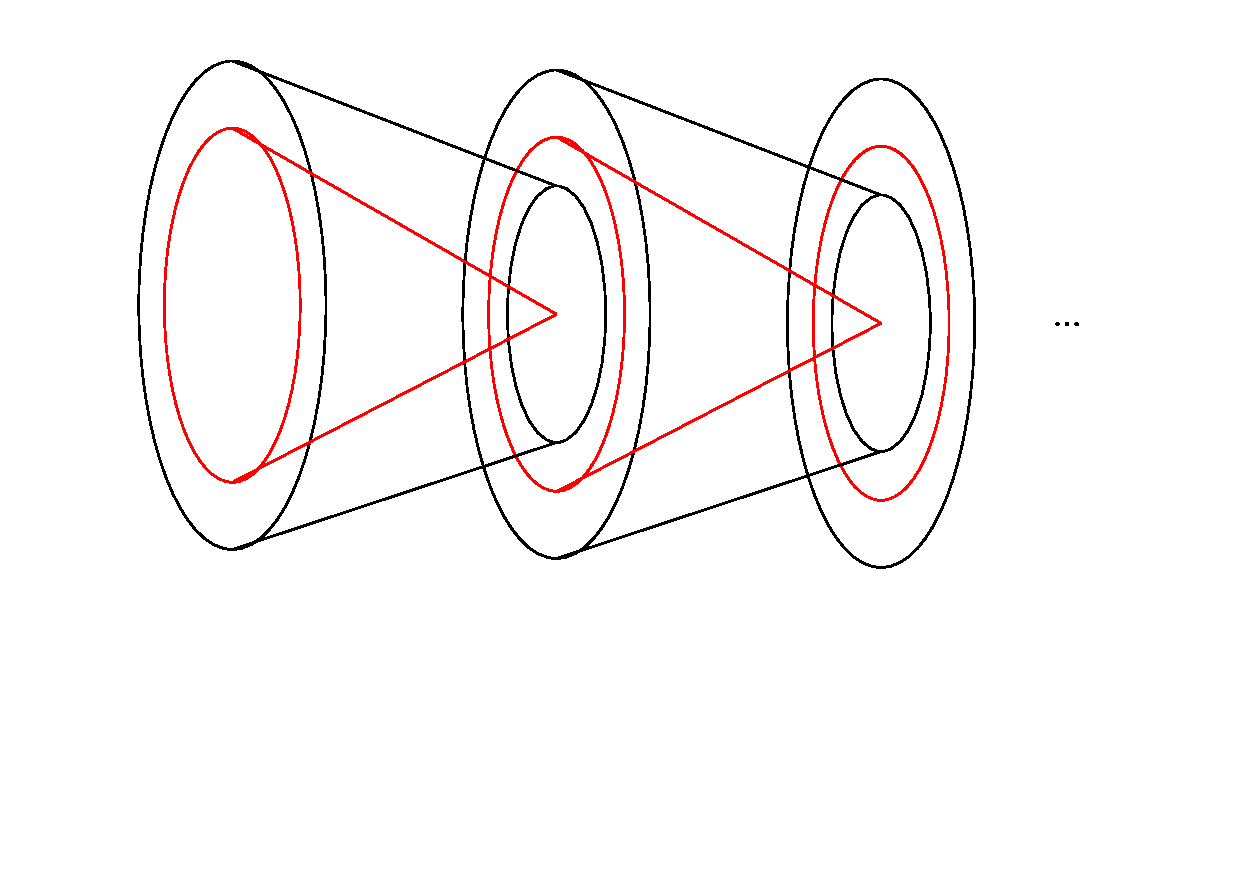
\includegraphics[scale=0.3]{img/1.pdf}
\end{figure}

$M_i$ is an $R$-module, $d^i$ is linear mapping and $$Ker(d^{i+1})\supseteq Im(d^i)$$ 

Thus we also have: $$d^{i+1}\circ d^i=0$$

The diagram is called exact if $$Ker(d^{i+1})=Im(d^i)$$
take a morphism $f:M\rightarrow N$ then 
\begin{itemize}
    \item $f$ is injective iff $$0\rightarrow M \stackrel{f}{\rightarrow} N$$ is exact
    \item $f$ is surjective iff $$M\stackrel{f}\rightarrow N\rightarrow 0$$ is exact
\end{itemize}
The first theorem of homomorphism 
$$\overline{f}:M/Ker(f)\stackrel{\cong}{\rightarrow}Im(f)$$
can be written as an exact sequence
$$0\rightarrow Ker(f)\stackrel{i}{\rightarrow}M\stackrel{f}{\rightarrow}Im(f)\rightarrow 0$$
More in general sequence like
$$0\rightarrow M_1\rightarrow M_2\rightarrow M_3\rightarrow 0$$
are called short exact sequences.
\section{Prop}
N is a R-module 
$$\_\otimes_RN:\forall M\quad M\mapsto M\otimes_RN$$
$$f:M\rightarrow P$$
$$f\otimes id_N:M\otimes_RN\rightarrow P\otimes_RN$$
Assume that we have a short exact (also complex)sequence of R-modules
$$0\rightarrow M_1\stackrel{f}{\rightarrow}M_2\stackrel{g}{\rightarrow}M_3\rightarrow 0$$
Then we apply $\_\otimes_RN$ to whole sequence
$$0\rightarrow M_1\otimes_RN\stackrel{f\otimes id_N}{\rightarrow}M_2\otimes_RN\stackrel{g\otimes id_N}{\rightarrow}M_3\otimes_RN\rightarrow 0$$
is a complex sequence if it's exact then we call N a flat R-module. One significant example's that the free module is flat.
\subsection{Example}
$$
\begin{aligned}
    0\rightarrow &\mathbb{Z}\stackrel{\mu}\rightarrow \mathbb{Z}&\stackrel{\pi}\rightarrow &\mathbb{Z}/2\mathbb{Z}\rightarrow0\\
    &x\mapsto 2x& &\\
    & &y \mapsto &2\mathbb{Z}+y
\end{aligned}
$$
Now apply $\_\otimes_\mathbb{Z}\mathbb{Z}/2\mathbb{Z}$
$$
\begin{aligned}
    0\rightarrow &\mathbb{Z}\otimes\mathbb{Z}/2\mathbb{Z}\stackrel{\mu\otimes id}\rightarrow &\mathbb{Z}\otimes\mathbb{Z}/2\mathbb{Z}\stackrel{\pi}\rightarrow &\mathbb{Z}/2\mathbb{Z}\otimes\mathbb{Z}/2\mathbb{Z}\\
    & x\otimes(2\mathbb{Z}+y)\mapsto &(2x)\otimes(2\mathbb{Z}+y) & \\
    & &z\otimes(2\mathbb{Z}+y)\mapsto &(2\mathbb{Z}+z)(2\mathbb{Z}+y)
\end{aligned}
$$
and 
$$
\begin{aligned}
    2x\otimes(2\mathbb{Z}+y) &=2(x\otimes 2\mathbb{Z}+y)\\
    &=x\otimes(2\mathbb{Z}+2y)\\
    &=x\otimes 2\mathbb{Z}\\
    &=0
\end{aligned}
$$
which is not injective, thus above isn't exact.
\section{Exercise(important)}
If $R=N$ then $\_\otimes_RN$ (where N is a finite dim vec space) is exact. Hint: use the basis.
\chapter{Tensor algebra}
Fix a vec space V (over K) of finite dimension
\section{Def}
We denote
$$
\begin{aligned}
    T_p^q:=&(V^\vee)^{\otimes p}\otimes V^{\otimes q}\qquad p,q\in \mathbb{N}\\
    =&\underbrace{V^\vee\otimes\cdots\otimes V^\vee}\limits_{p\text{ times}}\otimes \underbrace{V\otimes\cdots\otimes V}\limits_{q\text{ times}}\\
\end{aligned}
$$
An element of $T_p^q(V)$ is called a tensor of type $(p,q)$ (or a mixed tensor which is $p$-covariant and $q$-contravariant)

Let's denote:
$$T(V):=\bigoplus\limits_{q\in \mathbb{N}} T_0^q(V)$$
itemize some item in it:
$$\begin{aligned}
    &T_0^0(V)=K\\
    &T_1^0(V)=V^\vee\\
    &T_0^1(V)=V\\
    &T_1^1(V)=V^\vee\otimes V\cong\mathscr{L}(V;V)\\
    &T_2^0(V)=V^\vee\otimes V^\vee\cong (V\otimes V)^\vee\cong\mathscr{L}(V,V;K)
\end{aligned}$$
If you have a R-module M, then 
$$\bigotimes\limits_{n=0}^\infty M=\left\{(m_1,\cdots,m_n,\cdots):m_i\in M \text{ all but finite many }m_i=0\right\}$$
On $T(V)$ we have following operation:
$$
\begin{aligned}
    T_0^l(V)\times T_0^q(V)&\rightarrow T_0^{l+q}(V)\\
    ((x_1\otimes\cdots\otimes x_l),(y_1\otimes\cdots\otimes y_q))&= x_1\otimes\cdots\otimes x_l\otimes y_1\otimes\cdots\otimes y_q
\end{aligned}
$$

With this operation $T(V)$ becomes a $K$-algebra. It called the tensor algebra associated to $V$
\section{exterior product}
Let W be the two sided ideal of $T(V)$ generated by the element of the type $x\otimes x$
$$W=\left\{\sum\limits_{i(finite)}(y_1\otimes\cdots\otimes y_{m_i})\otimes(x_i\otimes x_i)\otimes(z_1\otimes\cdots\otimes z_{n_i})\right\} $$
With $x_j,y_j,z_j\in V$ and $n_i,m_j\in \mathbb{N}$
\section{Def}
The quotient algebra $$\bigwedge(V):=T(V)/W$$
is a K-algebra, which called the exterior algebra of V
$$
\begin{aligned}
    \pi: &T(V) &\rightarrow \bigwedge(V)\\
    &x_1\otimes\cdots\otimes x_n &\mapsto x_1\wedge\cdots\wedge x_n
\end{aligned}$$
This def is try to transform $\bigotimes$ to $\bigwedge$
\section{Notation}
$$\bigwedge(V)=\bigoplus \limits_{n\in\mathbb{N}} \bigwedge^n(V)$$
$$\bigwedge^n(V):=T^n_0(V)/W\cap T_0^n(V)$$
this is called $n$-fold exterior product
\section{Prop}
Let $\sigma\in \mathfrak{S}_n$ then $$x_1\wedge\cdots\wedge x_n=sgn(\sigma) x_{\sigma(1)}\wedge\cdots\wedge x_{\sigma(n)}$$
\subsection*{Proof}
Since any permutation can be written as the product of adjacent transpositions, it's enough to do the proof for $\sigma=(i,i+1)$
$$
\begin{aligned}
    0 &=(x_i+x_{i+1})\wedge(x_i+x_{i+1})\\
    &=(x_i\wedge x_i)+(x_i\wedge x_{i+1})+(x_{i+1}\wedge x_i)+(x_{i+1}\wedge x_{i+1})\\
    &=(x_i\wedge x_{i+1})+(x_{i+1}\wedge x_i)
\end{aligned}
$$
\section{Def}
Let E be an R-module and $f:E^n\rightarrow M$ a mapping.
We say that the pair $(M,f:E^n\rightarrow M)$ satisfies the universal property for the $n^{th}$-exterior power if
\begin{itemize}
    \item $M$ is an R-module, $f:E^n\rightarrow M$ is an n-linear mapping s.t.
    \begin{itemize}
        \item[ ] $\forall i\in \{1,\cdots,n-1\}$
        \item[] if$$x_i=x_{i+1}$$
        \item[] then$$f(x_1,\cdots,x_n)=0$$
        \item[] (alternating n-linear mapping)
    \end{itemize}
    \item If $P$ is an R-module and $\varphi:E^n\rightarrow P$ is an alternating mapping, then 
    $$\exists !\ \Phi:M\rightarrow P\text{ s.t. }\Phi\circ f=\varphi$$
\end{itemize}
\section{Def}
V is a K-vct space. A multi-linear mapping:
$$\begin{aligned}
    \varphi:V\times\cdots\times V\rightarrow W
\end{aligned}$$
is called skew-symmetric(alternating) if
$$\varphi(x_1,\cdots,x_n)=0\text{ when }\exists i\neq j:x_i=x_j$$
\section{Prop}
\label{VIII-46.8}
FIx a vct space V. For any alternating multi-linear mapping
$$s:\underbrace{V\times\cdots\times V}\limits_{n\text{ times}}\rightarrow W$$
when W is another vct space, there exists a unique linear mapping$$g_s:\bigwedge\limits^n(V)\rightarrow W$$
such that the following diagram commutes
$$\xymatrix{
    & V^n\ar[d]_t\ar[r]^s & W\\
    &T^n_0(V)\ar@{-->}[ur]^{f_s}\ar[d] &\\
    & \bigwedge\limits^n(V)\ar[uur]_{g_s}
}$$
\subsection*{Proof}
$$g_s(\sigma_1\wedge\cdots\wedge\sigma_n):=s(v_1,\cdots,v_n)$$
check the diagram is commutative
$$\xymatrix{
    &\mathcal{F}(V^n)\ar@{->>}[r]^t &T^n_0(V)\ar@{->>}[r]&\bigwedge\limits^n(V)\\
    &\{(\sigma_1,\cdots,\sigma_n)\}\ar@{|->}[r]&\{\sigma\otimes\cdots\times\sigma_n\}\ar@{|->}[r]&\{\sigma_1\wedge\cdots\wedge\sigma_n\}
}$$
\section{Remark/exercise}
The couple $\bigwedge\limits^nV$ with
$$V^n\rightarrow\bigwedge\limits^n(V)$$
that satisfies Prop \ref{VIII-46.8} is unique to unique isomorphism
\section{Prop}
Let V be a vct space of dimension n with a basis $\{e_1,\cdots,e_n\}$. Then $\bigwedge\limits^k(V)$ is a vct space with a basis given by $$\mathcal{B}=\{e_{i_1},\cdots e_{i_k}\big|\ 1\leq i_1<\cdots<i_k\leq n\}$$
In particular, $\bigwedge\limits^k(V)$ has dimension $\left(\begin{aligned}
    &n \\ &k
\end{aligned}
\right)$
\subsection{Proof}
$\mathcal{B}$ is clearly a generating set.The different part is to show that $\mathcal{B}$ is made of linearly independent elements.
$$I=\{i_1,\cdots,i_k\}$$ with $1\leq i_1<\cdots<i_k\leq n$, define
$$\begin{aligned}
    \varphi_I: V^n &\rightarrow K\\
    (e_{j_1},\cdots,e_{j_n})&\mapsto \left\{\begin{aligned}
        sgn(t) &\text{ if } \exists \tau\in S_I\quad\tau(j_m)=i_m\\
        0\quad &\text{otherwise} 
    \end{aligned}\right.
\end{aligned}$$
$\varphi_I$ is multilinear and alternating(skew-symm), hence it induce a linear mapping
$$
\begin{aligned}
    g_{\varphi_I}=\overline{\varphi_I}:\bigwedge\limits^k(V)  &\rightarrow K\\
    (e_{j_1}\wedge\cdots\wedge e_{j_k})&\mapsto \left\{\begin{aligned}
        sgn(t) &\text{ if } \exists \tau\in S_I\quad\tau(j_m)=i_m\\
        0 \quad&\text{otherwise} 
    \end{aligned}\right.
\end{aligned}
$$
With $\sigma\in\bigwedge\limits^n(V)$,assume that
$$0=\sigma=\sum\limits_{1\leq j_1<\cdots<j_k\leq n}\lambda_{j_1,\cdots,j_k}e_{j_1}\wedge\cdots\wedge e_{j_k}$$
By linearity$$0=\overline{\varphi}_I(\sigma)=\pm \lambda_I$$
Do it for any positive I this shows that any $\lambda_{j_1,\cdots,j_k}$ is zero.
\chapter{Determinant}
\section{Def}
Let V be a vct space of dimension n, then 
$$\det(V)=\bigwedge\limits^n(V)$$
is called the determinant of V. It is a vct space of dimension $1=\binom{n}{n}$ and a basis is given by $$e_1\wedge\cdots\wedge e_n$$
when $\{e_1,\cdots,e_n\}$ is a basis of V.
\subsection{Proof}
Let $f\in \mathscr{L}(V;V)$ then consider
$$\begin{aligned}
    \widetilde{f}: V^k &\rightarrow \bigwedge\limits^k V\\ 
    (\sigma_1,\cdots,\sigma_n) &\mapsto f(v_1)\wedge\cdots\wedge f(v_n)
\end{aligned}$$
This is multilinear and alternating. Therefore it induces a mapping
$$
\begin{aligned}
    g_{\widetilde{f}}=\bigwedge\limits^kf: &\bigwedge\limits^k(V) &\rightarrow\bigwedge\limits^k(V)\\
    &v_1\wedge\cdots\wedge v_k &\mapsto f(v_1)\wedge\cdots\wedge f(v_n)
\end{aligned}$$

Since $\det(V)$ has dim 1
$$\det (f):\sigma_1\wedge\cdots\wedge\sigma_n\mapsto {\underbrace{det_f}\limits_{\in K}}(v_1\wedge\cdots\wedge v_n)=f(v_1)\wedge\cdots\wedge f(v_n)$$
By abuse of notation we identity $$\det(f)=det _f$$
\section{Prop}
$f\in \mathscr{L}(V;V)$ is invertible iff $\det(f)\neq 0$
\subsection{Proof}
$f$ is not invertible iff $\{f(e_1),\cdots,f(e_n)\}$ is not a basis.

iff there's a non-trivial linear combination
$$\sum\limits_n\lambda_if(e_i)=0$$
After relabelling thee $e_i$ we can assume 
$$f(e_i)=\sum\limits_{i\geq 2}\mu_if(e_i)$$
$$\begin{aligned}
    \det (f)(e_1\wedge\cdots\wedge e_n)&=det_f\cdot(e_1\wedge\cdots\wedge e_n)\\
    &=(\sum\limits_{i\geq 2}\mu_if(e_i))\wedge f(e_1)\wedge\cdots\wedge f(e_n)\\
    &=\sum\limits_{i\geq 2}\mu_i(f(e_1)\wedge f(e_2)\wedge\cdots\wedge f(e_n))\\
    &=0
\end{aligned}$$
\section{Prop}
$$\det(f\circ g)=\det(f)\cdot\det(g)$$
\subsection*{Proof}
$$\begin{aligned}
    \det(f\circ g) &=(f\circ g)(e_1)\wedge\cdots\wedge(f\circ g)(e_n)\\
    &=f(g(e_1))\wedge\cdots f(g(e_n))\\
    &=(\det f)(g(e_1)\wedge\cdots g(e_n))\\
    &=\det f\cdot\det g(e_1\wedge\cdots g(e_n))
\end{aligned}$$
\section{Prop}
The determinant of $f$ is equal to the determinant of any matrix that represents $f$ with respect to a fixed basis. This doesn't depends on the choice of the basis.
\subsection*{Proof}
Fix a basis $\{e_1,\cdots,e_n\}$ of V. Then

$$\xymatrix{
    &v_i &V\ar[r]^f &V \\
    &e_i\ar@{|->}[u] &K^n\ar[u]_{\mathcal{B}}^\cong \ar[r]^{A_f} &K^n\ar[u]^\cong_{\mathcal{B}}
}
\Longrightarrow
\xymatrix{
    &\det(V)\ar[r]^{\det(f)} &\det(V)\\
    &\det(K^n)\ar[u]^{\bigwedge\limits^nb}\ar[r]^{\det(A_f)} &\det(K^n)\ar[u]^{\bigwedge\limits^nb}
}
$$ 

$A_f^{(v_1,\cdots,v_n)}$ is the matrix associated to $f$ with respect to the basis $\{v_1,\cdots,v_n\}$
suppose that $f(v_i)=\xi_{ij}v_i$. One we can see

$$A_f=\mathcal{B}^{-1}\circ f\circ\mathcal{B}(e_i)$$
$$\begin{aligned}
    \det (A_f) &((a_{11},a_{12},\cdots,a_{1n})\wedge(0,a_{22},a_{23},\cdots,a_{2n})\wedge\cdots\wedge(0,0,\cdots,1))
    \\ &=\mathcal{B}^{-1}(f(\mathcal{B}(a_{11},a_{12},\cdots,a_{1n})))\wedge\cdots\wedge\mathcal{B}^{-1(f(\mathcal{B}(0,0,\cdots,1)))}\\
    &=\xi_{1j}(0,\cdots,a_{1j},\cdots,a_{1n})\wedge\cdots\wedge\xi_{nj}(0,\cdots,a_{nj},\cdots,a_{nn})
\end{aligned}$$
(Einstein notation used for $j$)
We actually done the thing like
$$\left\lvert\begin{aligned}
    &a_{11}&a_{12}&\cdots&a_{1n}\\
    &0&a_{22}&\cdots&a_{2n}\\
    &\vdots&\vdots&\ddots&\vdots\\
    &0&0&\cdots&a_{nn}
\end{aligned}\right\rvert$$
\\compare the result with 
$$\det(f)(v_1\wedge\cdots v_n)=\xi_{1j}(v_1)\wedge\cdots\wedge\xi_{nj}(v_n)$$
We could find that $$\det(A_f)=\det(f)$$
Then we got $$\det(A)=\prod\limits_{i=1}^na_ii$$
\section{Prop}
If one column of $A$ can be expressed as a linear combination of other columns of $A$, then $$\det(A)=0$$
The columns are images of $\{e_1,\cdots,e_n\}$, means that $A(e_1),\cdots,A(e_n)$ are linearly dependent. Then $A$ is not an isomorphism, thus $\det(A)=0$.
If we exchange two columns of $A$, then $\det(A)$ changes sign.
\section{Prop}
Let $(a_ij)$ be a matrix of dimension $n\times n$. Then $$\det(A)=\sum\limits_{\sigma\in\mathfrak{S}_n}sgn(\sigma)\prod\limits_{i=1}^na_{i\sigma(i)}$$
\subsection*{Proof}
Let $\{v_1,\cdots,v_n\}$ be the columns of $A$, $v_i=A(e_i)$
$$\begin{aligned}
    \det(A)(e_1\wedge\cdots\wedge e_n) &=\sigma_1\wedge\cdots\wedge\sigma_n\\
    &=(\sum\limits_ia_{i1}e_i)\wedge\cdots\wedge(\sum\limits_ia_{in}e_i)\\
    &=\sum\limits_{\sigma\in\mathfrak{S}_n}\prod\limits_ia_{i\sigma(i)}\cdot e_{\sigma(1)}\wedge\cdots\wedge e_{\sigma(n)}\\
    &=(\sum\limits_{\sigma\in\mathfrak{S}_n}sgn(\sigma)\prod\limits_{i=1}^na_{i\sigma(i)})e_1\wedge\cdots\wedge e_n
\end{aligned}$$
\section{Corollary}
$$\det A=\det A^T$$
\subsection*{Proof}
$A^T=(\alpha_{ij}), A=(a_{ij})\quad \forall ij\ a_ij=\alpha_{ji}$
$$\begin{aligned}
    \det A^T &=\sum\limits_{\sigma\in\mathfrak{S}_n}sgn(\sigma)\prod\limits_{i=1}^n\alpha_{i\sigma(i)}\\
    &=\sum\limits_{\sigma\in\mathfrak{S}_n}sgn(\sigma)\prod\limits_{i=1}^na_{\sigma(i)i}\\
    &\overset{j=\sigma(i)}{=}\sum\limits_{\sigma\in\mathfrak{S}_n}sgn(\sigma^{-1})\prod\limits_{i=1}^na_{j\sigma^{-1}(j)}\\
    &\overset{sgn(\sigma)=sgn(\sigma^{-1})}{=}\det A
\end{aligned}$$
\section{Prop}
If you fix some basis on V and W, then $A_f$ is the matrix associated to $f^T$ is $A_f^T$
\section{?}
Fix  A of dimension of $n\times n$. Apply Gauss reduction and we get $A'$ a upper-triangle.

By the properties listed above$$\abs{\det A}=\abs{\det A'}$$
But on $A'$ the $\det$ is just the product of elements on then diagonal

Second method to compare the determinant is to use Gauss reduction and keep track of the row/column exchanges.
\section{Def}
Fix $A=(a_{ij}) (i,j)\in \{1,\cdots,n\}^2$. Denote with $A_{[i,j]}$ the matrix obtained removing the $i^{th}$ row and $j^{th}$ column of $A$. 
\section{Laplace expansion of the determinant}
Let $A=(a_{ij})$ then 
$$
\begin{aligned}
    \det A=&\sum\limits_{j=1}^n(-1)^{i+j}a_{ij}\det A_{[i,j]}\\
    &=\sum\limits_{i=1}^n(-1)^{i+j}a_{ij}\det A_{[i,j]}
\end{aligned}
$$
\subsection*{Proof}TEDIOUS

$$\xymatrix{
    &K^n\ar[r]^A &K^n\ar[d]_{p_i}\\
    & K^{n-1}\ar[u]^{t_j}\ar[r]^{A_{[i,j]}} &K^{n-1}
}$$
$\{e'_1,\cdots,e'_n\}$ is a standard basis of $K^n$
\\$\{e_1,\cdots,e_n\}$ is a standard basis of $K^{n-1}$
$p_i$ is the mapping that forgets about the i-th row.
$$p_i=(x_1,\cdots,x_i,\cdots,x_n)\mapsto(x_1,\cdots,\widehat{x_i},\cdots,x_n)=(x_1,\cdots,x_{i-1},x_{i+1},\cdots,x_n)$$
$$\tau_j(e_i)=\left\{\begin{aligned}e'_i &\text{ if } i<j\\ e_i &\text{ if } i\geq j\end{aligned}\right.$$

You can check that the above diagram is commutative. Now take $\bigwedge\limits^{n-1}$ of the diagram
$$\xymatrix{
    &\bigwedge\limits^{n-1}K^n\ar[r]^{\bigwedge\limits^{n-1}A} &\bigwedge\limits^{n-1}K^n\ar[d]_{\bigwedge\limits^{n-1}p_i}\\
    & \det(K^{n-1})\ar[u]^{\bigwedge\limits^{n-1}t_j}\ar[r]^{\det(A_{[i,j]})} &\det(K^{n-1})
}$$
$$\begin{aligned}
    \det(A) (e'_1,\cdots,e'_n)&=(-1)^{i-1}\det(A)(e'_i\wedge e'_1\wedge\cdots\wedge \widehat{e_i}\wedge\cdots\wedge e'_n)\\
    &=(-1)^{i-1} A(e'_i)\wedge A(e'_1)\wedge\cdots\wedge A(\widehat{e_i})\wedge\cdots\wedge A(e'_n)\\
    &=(-1)^{i-1}A(e'_i)\wedge\bigwedge\limits^{n-1}A(e'_1,\cdots,\widehat{e_i},\cdots,e'_n)=(*)
\end{aligned}$$
Let $$
\begin{aligned}
    \pi_j:K^n&\rightarrow K^n\\(x_1,\cdots,x_n)&\mapsto (0,\cdots,x_j,\cdots,0)
\end{aligned}
$$
Then $$A=\sum\limits_{i}(\pi_j\circ A)$$
It means that
$$
\begin{aligned}
    (*)&=(-1)^{i-1}A(e'_i)\wedge\sum\limits_j\bigwedge\limits^{n-1}(\pi_j\circ A)(e'_1,\cdots,\widehat{e_i},\cdots,e'_n)\\
    &=(-1)^{i-1}A(e'_i)\wedge\sum\limits_j\bigwedge\limits^{n-1}(\pi_j\circ A\circ \tau_i)(e_1,\cdots,e_{n-1})\\
    &=\sum\limits_{k,j}\left((-1)^{i-1}a_{kj}e'_k\wedge\bigwedge\limits^{n-1}(\pi_j\circ A\circ \tau_i)(e_1,\cdots,e_{n-1})\right)=(**)
\end{aligned}
$$
But $\pi_j(\cdot)$ is always collinear of $e_j$, so when $k=j$, the element in the sum is zero. We can remove the items that $k=j$
$$
\begin{aligned}
    \rho_k:=\tau_k\circ p_k: &K^n &\rightarrow &K^n\\ &(x_1,\cdots,x_n)&\mapsto &(x_1,\cdots,x_{k-1},0,x_{k+1},\cdots,x_n)
\end{aligned}$$
$\pi_k=id_{K^n}-\rho_k$ and $\sum\limits_{j\neq k}\pi_j=\rho_k$\\
Then
$$\begin{aligned}
    (**)&=\sum\limits_{k}(-1)^{i-1}a_kie'_k\wedge\bigwedge\limits^{n-1}\tau_k\circ\bigwedge\limits^{n-1}(p_k\circ A\circ \tau_i)(e_1\wedge\cdots\wedge e_{n-1})\\
    &=(***)
\end{aligned}$$
But by the diagram $$\bigwedge\limits^{n-1}(p_k\circ A\circ \tau_i)=\det A_{[i,k]}$$
$$\bigwedge\limits^{n-1}\tau_k(e_1\wedge\cdots\wedge e_{n-1})=e'_1\wedge\cdots\wedge \widehat{e_k}\wedge\cdots\wedge e'_n$$
Thus
$$\begin{aligned}
    (***)&=\sum_k(-1)^{i-1}a_{ki}\det (A_{[k,i]})(e'_k\wedge e'_1\wedge\cdots\wedge \widehat{e_k}\wedge\cdots\wedge e'_n)\\
    &=\sum\limits_{k}(-1)^{i+k}a_{ki}\det(A_[k,i])e'_1\wedge\cdots\wedge e'_n
\end{aligned}$$
\chapter{The Structure of Linear Mappings}
\section{Theorem}
Let $f:V\rightarrow W$ be a linear mapping between vct spaces of finite and same dim. Then:
\begin{itemize}
    \item [1] there exists decomposition $V=V_0\oplus V_1$ and $W=W_1\oplus W_2$ such that $V_0=\ker f$ and $f$ includes an isomorphism between $V_1$ and $W_1$(namely $f\mid_{V_1}$)
    \item [2] There exists basis in V nad W s.t. the associated matrix $A_f=a_{ij}$ satisfies $\forall 1\leq i\leq r,\exists r\leq n$ have $a_{ii}=1$ and  have $a_{ij}=0$ elsewhere
    \item [3] Let $A$ be a $m\times n$ matrix Then there exists two square matrices (with $\det\neq 0$) $B$ and $C$ of dim $m\times m$ and $n\times n$ and a num $r\leq min(m,n)$ s.t. $BAC$ has the form in $(2)$ Moreover the number $r$ is unique $r=rank(A)$
    
\end{itemize}

\section{Def}
Let $F:V\rightarrow V$ be a linear mapping. A subspace $V_0\subseteq V$ is said to be an invariant subspace of $F$ is $F(V_0)\subseteq V_0$
\section{Def}
A linear mapping $f:V\rightarrow V$ (finite dim) is diagonalizable if the following equivalent conditions are satisfied
\begin{itemize}
    \item [1] $V$ decomposes as a direct sum of one-dimensional invariant subspace of $f$
    \item [2] There exists a basis of $V$, in which the matrix $A_f$ is diagonal.
\end{itemize}
\subsection*{Proof of equivalence}
\begin{itemize}
    \item [2 $\Rightarrow$ 1]Assume that in the base $\{v_1,\cdots,v_n\}$ , we have $A_f=\left(\begin{aligned}
        &\lambda&&\\ &&\ddots&\\ &&&\lambda_n\end{aligned}\right)$ by the familiar diagram
        $$\xymatrix{&V\ar[r]^f &V\\ &K^n\ar[u]^b\ar[r]^{A_f} &K^n\ar[u]^b}$$$$f(v_i)=b\circ A_f(e_i)=b(\lambda_ie_i)=\lambda_iv_i\in\left<v_i\right>$$
        So $$V=\left<v_1\right>\oplus\cdots\oplus\left<v_n\right>$$
    \item [1 $\Rightarrow$ 2]Assume that $V=\left<v_1\right>\oplus\cdots\oplus\left<v_n\right>$, where $f(\left<v_i\right>)\subseteq\left<v_i\right>$
    , then $\{v_1,\cdots,v_n\}$ forms a basis of $V$\\
    Consider the previous diagram
    $$A(e_1)=b^{_1}\circ f\circ b(e_i)=b^{-1}(f(v_i))=b^{-1}(\lambda_iv_i)=\lambda_ie_i$$
\end{itemize}
\subsection{Example}
Take $$A:\mathbb{R}^2\rightarrow\mathbb{R}^2\quad A=\left(\begin{aligned}&\cos\theta &\sin\theta\\ &-\sin\theta&\cos\theta\end{aligned}\right)$$ $A$ is not diagonalizable.
\section{Def}
Let $L$ be a one-dimensional invariant subspace of $f:V\rightarrow V$ . Then $F\mid_L$ is a multiplication by a scalar $\lambda\in K$. Such $\lambda$ is called eigenvalue of $f$. Anon-zero vector $v\in V$ is called an eigenvector of $V$ if $\left<v\right>$ is an invariant subspace of $f$
\section{Remark}
$$\xymatrix{ &\{eigenvectors\}\ar[r]&\{\text{Set of invariant subspaces of dim 1}\}\ar[r] &K\\
&&v\ar@{|->}[r]\left<v\right>\ar@{|->}[r]&eigenvalue
}$$
This mapping is generally NOT injective. If $V$ is an eigenvector, then $\mu v$ is also an eigenvector, $\forall \mu\in K$
\section{Remark/exercise}
Assume that $f$ is diagonalizable and $A_f$ is a diagonal matrix that represents $f$ Then $A_f$ is unique up to permutation of the columns in the diagonal.
$$V=\left<v_1\right>\oplus\cdots\oplus\left<v_n\right>=\left<v_{\sigma(1)}\right>\oplus\cdots\oplus\left<v_{\sigma(n)}\right>\quad \sigma\in \mathfrak{S}_n$$
\section{Def}
V a vector space over K $dim(V)=n,f\in \mathscr{L}(V;V)$ let $A_f$ be an associated matrix (in any basis) the mapping
$$\begin{aligned}
    P: &K &\rightarrow& K\\&t&\mapsto& \det(tI_n-A_f)
\end{aligned}$$
This is a polynomial in $K[t]$ (with degree $n$)
\section{Lemma}
$P(t)$ is a monic polynomial of degree $n$
\subsection*{Proof}
$$P(t)=\det(tI_n-A_f)=\sum\limits_{\sigma}sgn(\sigma)\prod\limits_{i=1}^n(t\delta_{i\sigma(i)}-A_{i\sigma(i)})$$
The only item giving $t^n$ is when $\sigma=id$
\section{Theorem}
Use the notations introduced before
\begin{itemize}
    \item[1]$P(t)$ doesn't depends on $A_f$ (if you change basis, $P(t)$ does not change)
    \item[2] Any eigenvalue of $f$ is a root of $P(t)$. Conversely any $K$-root of $P(t)$ is an eigenvalue of $f$
\end{itemize}
\subsection*{Proof}
\begin{itemize}
    \item [1] Put $A=A_f$ and $A'$ be another representation of $f$ Then $A'=B^{-1}AB$ where $B$ invertible $n\times n$ matrix.
    $$
    \begin{aligned}
        \det(tI_n-A')&=\det(tI_n-B^{-1}AB)\\ &=\det(B^{-1}(tI_n)B-B^{-1}AB)\\ &=\det(B^{-1}(tI_n-A)B)\\ &=\det(tI_n-A)
    \end{aligned}
    $$
    \item[2] Let $\lambda\in K$ be a $K$-root of $P(t)$, then $$\det(\lambda I_n-A_f)=0=P(\lambda)$$
    $\lambda I_n-A_f$ is not invertible, $\exists v\neq0\in \ker(\lambda I_n-A_f)$ s.t. $$A_f(\sigma)=\lambda\sigma$$ then $\sigma$ is an eigenvector

    Vice versa if $\sigma\neq0,f(\sigma)=\lambda\sigma,\sigma\in Ker(\lambda I_n-A_f)$,$\det(\lambda I_n-A_f)=0=P(t)$ 
\end{itemize}
\section{Def}
The polynomial $P(t)$ will be  denoted by $P_f(t)$. It's called the characteristic polynomial of $f$
\section{Corollary}
If $P_f(t)$ splits with  no repeated roots, then $f$ is diagonalizable.
\subsection*{Proof}
Natural$$\left<\sigma_1\right>,\cdots\left<\sigma_n\right>$$
are all different then
$$V=\left<\sigma_1\right>\oplus\cdots\oplus\left<\sigma_n\right>$$
\section{Remark}
The inverse version does not hold.
\section{Def: Jordan block}A matrix of form
$$J_r(\lambda)=\begin{pmatrix}
    \lambda &1&&&\\
    0&\lambda&1&&\\
    &&\ddots&\ddots\\
    &&& &1\\
    &&&&\lambda\\
\end{pmatrix}\in M_{r\times r}(K) \quad r\geq 1$$ is called a Jordan block (element $\lambda\in K$ is $J_1(\lambda)$)
\section{Def: Jordan matrix}
A Jordan matrix if a matrix of form
$$J=\begin{pmatrix}
    J_{r_1}(\lambda_1)&\cdots&\\
    &J_{r_2}(\lambda_2)&&\\
    &&\ddots&
\end{pmatrix}$$
\section{Example}
Let $V_n(\lambda)$ be the vector space of complex functions:
$$F(x):=e^{\lambda x}f(x)$$ where $\lambda\in \mathbb{C},f\in \mathbb{C}[x]\leq n-1$

Verify that $V_n(\lambda)$ is a vector space of dim $n$
$$\begin{aligned}
    \frac{d}{dx}(e^{\lambda x} f(x)) &=\lambda e^{\lambda x}f(x)+e^{\lambda x}f'(x)\\ &=e^{\lambda x}(\lambda f(x)+f'(x))
\end{aligned}$$
$\frac{d}{dx}\in\mathscr{L}(V_n(\lambda);V_n(\lambda))$ Consider$$v_{i+1}=\frac{x^i}{i!}e^{\lambda x}$$
Show that $\{v_0,\cdots,v_{n-1}\}$ forms a basis of $V_n(\lambda)$
$$\begin{aligned}
    \frac{d}{dx}v_{i+1} &=\lambda v_{i+1}+\frac{x^{i-1}}{(i-1)!}e^{\lambda x}\\ &=\lambda v_{i+1}+v_i
\end{aligned}$$
Then 
$$A_{\frac{d}{dx}}=\begin{pmatrix}
    \lambda& & &\\
    1&\ddots&&\\
    &\ddots&&\\
    &&1&\lambda
\end{pmatrix}=(J_n(\lambda))^T$$
\section{Def}
Let $a_0+a_1t+\cdots+a_nt^n= Q(t)\in K[t]$, then for $f\in \mathscr{L}(V;V)$ we define 
$$Q(f):=a_0id_V+a_1f+a_2f^{\circ 2}+\cdots+a_nf^{\circ n}$$
\begin{itemize}
    \item[Remark]
From now on we write
$$f^{\circ k}=f^k$$
\end{itemize}
these are operations in $\mathscr{L}(V;V),+,\circ$

we say that $Q$ annihilates $f$ if $Q(f)=0$
\section{Prop}
\label{Prop.48.17}
Let $f\in \mathscr{L}(V;V)$. There exists a polynomial $Q\in K[t]\setminus\{0\}$ that annihilates $f$ (i.e. $Q(f)=0$)
\subsection*{Proof}
$$dim(\mathscr{L}(V;V))=n^2$$
Hence the mapping $\underbrace{id_V,f^2,\cdots,f^{n^2}}\limits_{n^2+1\text{ mappings}}\in\mathscr{L}(V;V)$ are linear dependent. There exists a non-trivial linear comb:
$$\lambda_0id_V+\lambda_1f+\cdots+\lambda_{n^2}f^{n^2}=0$$
So, take $$Q(t)=\lambda_0+\lambda_1t+\cdots+\lambda_{n^2}t^{n^2}$$ This show that $Q\neq0$ and $Q(f)=0$
\subsection*{Remark}The proof of this proposition also gives the degree of a polynomial that annihilates $(\leq n^2)$
\section{Def}
Let $m(t)\in K[t]\setminus\{0\}$ be a monic polynomial of minimal degree that annihilates $f\in \mathscr{L}(V;V)$. Then $m(t)$ is called minimal polynomial of $f$

And by prop above (\ref{Prop.48.17}), $m(t)$ exists.
\section{Prop}
If $m(t)$ is minimal polynomial of $f$, then $m(t)$ is unique.
\subsection*{Proof}
Assume that $m_1(t)$ is another minimal polynomial of $f$. Then $m-m_1(t)\in K[t]$
$$(m-m_1)(f)=m(f)-m_1(f)=0-0=0$$
Now $m$ and $n$ are both monic, so $$deg(m-m_1)<deg(m)=deg(m_1)$$
$m-m_1$ is a polynomial of $deg<deg(m)$ that annihilates $f$, thus $$m-m_1=0\in K[t]$$
\section*{Notation}
Form now no we denote the minimal polynomial of $f$ by $m_f$
\subsection*{Question}
$f\in\mathscr{L}(V;V)$ we have $P_f,m_f\in K[t]$.

What is the relationship between $P_f$ and $m_f$?  
\section{Prop}
Let $Q\in K[t]\setminus\{0\}$ be a polynomial that annihilates $f$. Then $m_f\mid Q$ 
\subsection*{Proof}
Let $$Q(t)=m_f(t)\cdot s(t)+\mathbcal{r}(t)$$
such that $deg(\mathbcal{r})< deg(m_f)$. So
$$0=Q(f)=m_f(f)s(f)_\mathbcal{r}(f)=0+\mathbcal{r}(f)\Rightarrow \mathbcal{r}(f)=0$$
But since $m_f$ is the minimal polynomial of $f$, then $$\mathbcal{r}(t)=0$$
\section{Def}
Let $A$ be a matrix of dim $n\times n$ and $$M_{ij}:=(-1)^{i+j}\det(A_{[i,j]})\quad \forall (i,j)\in \{1,\cdots,n\}^2$$
In this expression $$\det(A_{[i,j]})$$ is called the $(i,j)$-monic of $A$.

Then we define$$Adj(A):=(M_{ij})^T$$ called adjugate matrix of $A$
\section{Prop}
$$Adj(A)\cdot A=A\cdot Adj(A)=\det(A)\cdot I_n$$
\subsection*{Proof}
use Laplace expansion.
\section{Theorem: Cayley-Hamilton Theorem}
The characteristic polynomial $P_f$ annihilates $f$

Consequence: $m_f\mid P_f$
\subsection*{Proof}
Let $A=A_f$ any matrix that represents $f$. COnsider $$B:=Adj(tI_n-A)$$
$B$ is a matrix with coefficient in $K[t]$($B\in M_{n\times n}(K[t])$)

Then$$(tI_n-A)\cdot B=\det(tI_n-A)\cdot B==P_f(t)\cdot I_n$$
We can decompose $B$ in the following way
$$B=\sum\limits_{i=0}^{n-1}t^iB_i\quad B_i\in M_{n\times n}(K)$$
We have at most $n-1$, because the coefficient of $B$ have degree at most $n-1$

(Any entry Adj is a det ogf a matrix of dim $(n-1)\times(n-1)$)
$$
\begin{aligned}
    P_f(t)I_n &=(tI_n-A)\cdot\sum\limits_{i=0}^{n-1}t^iB_i\\
    &=(\sum\limits_{i=0}^{n-1}tI_n\cdot t^iB_i)-(\sum\limits_{i=0}^{n-1}A\cdot t^iB_i)\\
    &=\sum\limits_{i=0}^{n-1}t^{i+1}B_i-\sum\limits_{i=0}^{n-1}A\cdot t^iB_i\\
    &= t^nB_{n-1}+\sum\limits_{i=0}^{n-1}t^i(B_{i-1}-AB_i)-AB_0
\end{aligned}
$$Recall that $P_f(t)\cdot I_n=t^nI_n+ c_{n-1}t^{n-1}I_n+\cdots+c_1tI_n+c_0I_n$
$$
\begin{aligned}
    &t^nI_n+c_{n-1}t^{n-1}I_n+\cdots+c_0I_n\\=&\cdots\\=&t^nB_{n-1}+\sum\limits_{i=1}^{n-1}t^i(B_{i-1}-AB_i)-AB_0
\end{aligned}
$$
Then we can compare the coefficients:
$$B_{n-1}=I_n$$
$$B_{i-1}-AB_i=c_iI_n\quad 1\leq i\leq n-1$$
$$-AB_0=c_0I_n$$
Multiply by $A^i\ 0\leq i\leq n$
$$A^nB_{n-1}+\sum\limits_{i=1}^{n-1}(A^iB_{n-1}-A^{i+1}B)-AB_0=A^n+c_{n-1}A^{n-1}+\cdots+c_1A+c_0I_n$$
Now the LHS we have a telescopic sum and got
$$0=P_f(A) \Leftrightarrow 0=P_f(f)$$
\section{Example}
\begin{itemize}
    \item[(a)] $m_f$ and $P_f$ are in general different. let $f=id_V,(dim V=n)$
    $$P_f(t)=(t-1)^n\quad m_f(t)=t-1$$
    \item[(b)]Assume $f:V\rightarrow V(dim V=\mathbcal{r})$ and $A_f=J_\mathbcal{r}(\lambda)$. Then
    $$P_f(t)=(t-\lambda)^\mathbcal{r}$$
    Moreover $$J_\mathbcal{r}(\lambda)=\lambda I_\mathbcal{r}+J_\mathbcal{r}(0)$$ and $$J_\mathbcal{r}(o)^k=\begin{pmatrix}
        \overbrace{0\cdots 1}\limits^{k+1}&&\\&\ddots&\\ &&1\\&&\vdots\\&&0
    \end{pmatrix}$$ if $k\geq\mathbcal{r},J_\mathbcal{r}(o)^k=0$
    $$(J_\mathbcal{r}(\lambda)-\lambda I_n)^k=(\lambda I_\mathbcal{r}-J_\mathbcal{r}(0)-\lambda I_\mathbcal{r})^k=J_\mathbcal{r}(0)^k\neq 0$$ if $0\leq k\leq\mathbcal{r}-1$\\We know that $m_f\mid (t-\lambda)^\mathbcal{r}$(by Cayley-Hamilton), $m_f$ must be of the type $$m_f=(t-\lambda)^k$$
    But the only possibility is $k=\mathbcal{r}$, thus$$m_f=P_f$$
\end{itemize}
\section{Theorem}Let $f\in\mathscr{L}(V;V)$ when $V$ is a vector space of dim $n$, over an algebraically closed field.\\Then
\begin{itemize}
    \item [(1)]$f$ can be represented by a Jordan matrix
    \item [(2)]This above matrix is unique up to permutation of the Jordan blocks
\end{itemize}


(Note that a field $K$ is algebraically closed if any non-zero polynomial has a root in $K$)
\section{Def}
Let $f\in\mathscr{L}(V;V)$ and let $\lambda\in K$. A vector $w\in V\setminus\{0\}$ is called a root vector of $f$ corresponding to $\lambda$, if there exists $\mathbcal{r}\in\mathbb{N}$ s.t. $$(f-\lambda id_V)^\mathbcal{r}(w)=0$$
\subsection*{Remark}
Eigenvector are root vectors (corresponding to their eigenvalues) take $\mathbcal{r}=1$

\subsection*{Remark}
Let $J_\mathbcal{r}(\lambda)$ be a Jordan block. Then any $\sigma\in V$ is a root vector of $f$ corresponding to $\lambda$. In fact:
$$(J_\mathbcal{r}(\lambda)-\lambda I_n)^m=0\quad\text{if }m\geq\mathbcal{r}$$
\section{Prop}
\label{Prop 48.27}
Let $K$ be an algebraically closed field. Let $\lambda_1,\cdots,\lambda_k$ be all of distinct eigenvalues of $f(k\geq1)$, then 
$$V=\bigoplus\limits_{i=1}^kV(\lambda_i)$$
\subsection*{Proof}
Since $K$ is algebraically closed, then
$$P_f(t)=\prod\limits_{i=1}^k(t-\lambda_i)^{r_i}\in K[t]$$
Consider $$F_i(t):=P_f(t)\cdot(t-\lambda_i)^{-r_i}\in K[t]$$
Then we define $$f_i:=F_i(f)\in\mathscr{L}(V;V),V_i=Im f_i$$
\subsubsection{Setp 1}
We want to prove that $$(f-\lambda_i Id_V)^{\circ r_i}(V_i)=0\Leftrightarrow V_i\subseteq V(\lambda_i)$$
which got from 
$$(f-\lambda_i Id_V)^{\circ r_i}\circ(f_i)=(t-\lambda_i)^{r_i}(f)\circ F_i(f)=P_f(f)=0$$
\subsubsection{Step 2}
We want to prove that $$V=\bigoplus\limits_{i=1}^kV_i$$
Since the polynomials $F_i(t)$ are coprime, then
$$\exists G_i(t)\in K[t]\text{ s.t. }\sum\limits_{i=1}^k F_i(t)G_i(t)=1$$
Let $f$ substitute for $t$
$$\sum\limits_{i=1}^k F_i(f)G_i(f)=Id$$
take $v\in V$
$$\sum\limits_{i=1}^k f_i\circ G_i(f)(v)=v$$
$$\xymatrix{
    &&&\bigoplus\limits_{i=1}^kV_i&&\\
    &V_1\ar[urr]_i&V_2\ar[ur]_i&\cdots&V_{k-1}\ar[ul]^i&V_k\ar[ull]^i\\
    &V\ar@{}[r]|=\ar[u]^{f_1\circ G_1(f)}&V\ar[u]^{f_2\circ G_2(f)}\ar@{}[r]|=&\cdots\ar@{}[r]|=&V\ar@{}[r]|=\ar[u]^{f_{k-1}\circ G_{k-1}(f)}&V\ar[u]^{f_k\circ G_k(f)}
}$$
$i$ is the inclusion mapping.
\subsubsection{Step 3}
We want to show that $$V_i\cap (\sum\limits_{i\neq j}V_j)=\{0\}$$
Let $v$ be a vector in this intersection. Then by calculation,
$$(f-\lambda_i)^{r_i}(v)=0$$
$$F_i(f)(v)=\prod\limits_{i\neq j}(f-\lambda_j)Id^{\circ r_i}(v)=0$$
Now $(t-\lambda_i)^{r_i}$ and $F_i(t)$ are coprime. Then there exists $G_1(t)$ and $G_2(t)$  such that:
$$G_1(t)(t-\lambda_i)^{t_i} +G_2(t)F_i(t)=1$$
substitute $f$ instead of $t$ by 
$$G_1(f)\circ (f-\lambda_i Id_V)^{\circ r_i}+G_2(f)\circ F_i(f)=Id_V$$
Then apply to $v=\sum\limits_{j\neq i}v_j,v_j\in V_j$
$$G_1(f)\circ (f-\lambda_i Id_V)^{\circ r_i}(v) +G_2(f)\circ F_i(f)(v)=v=0$$
\subsubsection{Step 4}
We want to show that $$V_i=V(\lambda_i)$$
By step 1 we get $$V_i\subseteq V(\lambda_i)$$Take $v\in V(\lambda_i)$, write it as $$v=v'(\in V(\lambda_i))+v''(\in \bigotimes\limits_{j\neq i}V_j)$$
By step 3, $$v''=v-v'\in V(\lambda_i)$$
Use same trick,substitute f for t and calculate in $v''$
$$v''=0$$
\section{Def}
Let $f\in  \mathscr{L}(V;V)$. Then $f$ is said to be nilpotent if there exists $t\in \mathbb{N}$ that $f^t=0$
\section{Lemma}
Let $f$ be a nilpotent mapping, then $$Ker(f)=\{\text{set of eigenvalues of }f\}$$
\subsection*{Proof}
Let $v\in Ker(f)$ then $v$ is an eigenvector with eigenvalue$=0$

Let $v$ be an eigenvector, then $\forall m\geq r$
$$0=f^m(v)=f^{m-1}(f(v))=f^{m-1}(\lambda v)=\lambda^m v\Rightarrow \lambda^m=0\Rightarrow \lambda=0$$
\section{Lemma}
Let $f$ be a nilpotent mapping, then $Ker (f)\neq\{0\}$
\subsection*{Proof}
Let $\mathbcal{r}$ be the minimal integer s.t. $f^\mathbcal{r}=0$ then
$$f^{\mathbcal{r}-1}(V)\subseteq Ker(f)$$
but $f^{\mathbcal{r}-1}(V)\neq\{0\}$ because of the minimality of $\mathbcal{r}$
\subsection*{Remark}
Another way to prove is that $Q(t)=t^\mathbcal{r}$ annihilates $f$. So $m_p=t^{\mathbcal{r}'},\mathbcal{r}'\leq\mathbcal{r}$ Note that 0 is a root of $m_f$, by Cayley-Hamilton theorem, 0 is an eigenvalue $f(x)=0\cdot x=0$ for some $x\neq0$
\section{Jordan matrix of form $J_\mathbcal{r}(0)$}
Recall that $$J_\mathbcal{r}(0)^k=0\text{ if }k\geq \mathbcal{r}$$
Then the Jordan matrix $$\begin{pmatrix}
    J_{\mathbcal{r}_1}(0)&&\\
    &J_{\mathbcal{r}_2}(0)&&\\
    &&\ddots
\end{pmatrix}$$
Are nilpotent mappings since each block is nilpotent. Take one block
$$J_\mathbcal{r}(0)=\begin{pmatrix}
    0&1&&\\
    &0&1&&\\
    &&\ddots&\ddots
\end{pmatrix}\quad=\left\{\begin{matrix}
    e_1\mapsto 0\\e_2\mapsto 1\\\vdots\\e_\mathbcal{r}\mapsto e_{\mathbcal{r}-1}
\end{matrix}\right.$$
We represent the action of a Jordan block on a basis as the following diagram
$$\underbrace{e_\mathbcal{r}\rightarrow e_{\mathbcal{r}-1}\rightarrow e_{\mathbcal{r}-2}\rightarrow \cdots \rightarrow e_1\rightarrow 0}\limits_{\text{lenth of the block}(\mathbcal{r})}$$$e_1$ is the one which mapped to 0 (thus an eigenvector)

Given $f\in \mathscr{L}(V;V)$ if we find a basis on which $f$ acts as in the previous diagram. Then we have found a Jordan basis made of  blocks of the type "$J_\mathbcal{r}(0)$"
\section{Theorem}
Let $f\in\mathscr{L}(V;V)$ be a nilpotent mapping, then there exists a Jordan basis for $f$ that gives a Jordan matrix made of blocks of the type $J_\mathbcal{r}(0)$
\subsection*{Proof}
We need to find a basis that induces a diagram of the type $\mathcal{D}:$(dots in the diagram are basis)
$$\xymatrix{
    \cdot\ar[d]&&&&\cdot\ar[d]\\
    \cdot\ar@{}[d]|\vdots&\cdot\ar[d]&&&\cdot\ar[d]\\
    \cdot\ar[d]&\cdot\ar[d]&\cdot\ar[d]&\cdots&\cdot\ar[d]\\
    \cdot\ar[d]&\cdot\ar[d]&\cdot\ar[d]&&\cdot\ar[d]\\
    0&0&0&&0
}$$
(Last line of dots naturally be eigenvectors)

We work by induction on $dim(V)$. If $dim(V)=1$, then $$f=\mu(\cdot),f^\mathbcal{r}=0\ \mu^\mathbcal{r}v=0\ \forall v\Rightarrow \mu=0$$
But $0=J_1(0)$. Assume that the theorem is true for $dim(V)<n$ Let $$V_0=Ket f=\{\text{the set of eigenvalues}\}\cup\{0\}$$ Since $f$ is nilpotent $$dim(V_0)\geq 1$$. Therefore$$dim(V/V_0)<n$$ So define the following mapping
$$
\begin{aligned}
    \overline{f}: &V/V_0 &\rightarrow &V/V_0\\&\overline{\sigma}=V_0+\sigma&\mapsto &V_0+f(v)=\overline{f(v)}
\end{aligned}$$
$$\overline{f}\cdot\overline{\sigma}\mapsto\overline{f(v)}$$
is nilpotent
We use the induction hypothesis

We have a Jordan basis for $\overline{f}$, so we have elements $\overline{\sigma_1},\cdots,\overline{\sigma_m}\in V/V_0$ that give a diagram $\overline{\mathcal{D}}$:
$$\xymatrix{}$$
Now left $\overline{\sigma_i}$ to some element $\sigma_i\in V$ choose $\sigma_i\in V$ s.t $\sigma+V_0=\overline{\sigma_i}$Now start applying $f$ to these elements $\sigma_i\neq 0$

$$v_i\rightarrow f(v_i)\rightarrow\cdots\rightarrow f^{b_i-1}(v_i)\rightarrow f^{b_i}(v_i)$$


When $b_i$ is the first integer such that $$\overline{f}^{b_i}(\overline{v_i})=0$$
This means that $$f^{b_i}(v_i)\in V_0$$ hence $f^{b_i}(\sigma_i)$ is an eigenvalue for ? Consider now the vector subspace generated by $f^{b_1}(v_1),f^{b_2}(v_2),\cdots,f^{b_m}(v_m)$$$\left<f^{b_1}(v_1),\cdots,f^{b_m}(v_m)\right>\subseteq V_0$$
Extract a basis and complete to a basis of $V_0$. The new vectors are denoted by $u_1,\cdots, u_t$

We want to prove that the elements of $\mathcal{D}$ form $\cdot$ basis of $V$
\subsubsection*{1}The elements of $\mathcal{D}$ generate $V$ let $\sigma\in V$$$\overline{\sigma}=\sum\limits_{i=1}^m\sum\limits_{j=0}^{b_i-1}a_ij\overline{f^j}(\overline{v_i})$$
Now I use the properties of $\overline{f}$$$\begin{aligned}
    &\overline{f}(\overline{v_i})=\overline{f(v_i)}\\ &\overline{f}(\overline{f(v)})=\overline{f(f(v))}
\end{aligned}$$
then $$\overline{\sigma}=\overline{\sum\limits_{i=1}^m\sum\limits_{j=0}^{b_i-1}a_ij{f^j}({v_i})}$$
which gives
$$\sigma-\sum\limits_{i=1}^m\sum\limits_{j=0}^{b_i-1}a_ij{f^j}({v_i})\in V_0$$
this finishes. We know that
$$V_0=\left<f^{b_1}(v_1),\cdots,f^{b_m}(v_m),u_1,\cdots,u_t\right>$$
\subsubsection*{2}
We need to prove that the elements of $\mathcal{D}$ are linearly independent
\begin{itemize}
    \item [a] We show that the elements of the bottom row are linearly independent$$\sum\limits_{i=1}^ma_if^{b_i}(v_i)+\sum\limits_{i=1}^tc_iu_t=0$$
    This is a non-trivial linear comb.
    
    The first observation is that $b_i=0$. Because if $b_j\neq0$ $$u_j=\frac{\sum\limits_{i=1}^ma_if^{b_i}(v_i)}{\sum\limits_{i=1}^tc_i}$$ But $u_1,\cdots,u_t$ were an extension of a basis. So $$0=\sum\limits_{i=1}^ma_if^{b_i}(v_i)=f(\sum\limits_{i=1}^ma_if^{b_i-1}(v_i))\Rightarrow(\sum\limits_{i=1}^ma_if^{b_i-1}(v_i))\in V_0$$
    It means that
    $$\sum\limits_{i=1}^ma_i\overline{f}^{b_i}(v_i)=0\Rightarrow a_i=0\forall i$$
    \item [b] If there is a non-trivial linear comb that equals to 0. For elements of $\mathcal{D}$. We can write it as linear comb of elements of the last row
    $$f(\sum\limits_{i=1}^m\sum\limits_{j=1}^{b_i}a_{ij}f^j(v_i)+\sum\limits_{i=1}^tc_iu_t)=0$$
    By applying $f$ many times we get a linear comb of elements of the last row.

    By point a,finished.
\end{itemize}
\section{Prop}
The Jordan matrix that represents a nilpotent mapping $f\in \mathscr{L}(V)$ is unique to permutations of the blocks.
\subsection*{Proof}
Recall that a Jordan basis of $f$ is given be diagram of the type $\mathcal{D}$
$$\xymatrix{
    \cdot\ar[d]&&&&\\
    \cdot\ar[d]&\cdot\ar[d]&&\\
    \cdot\ar[d]&\cdot\ar[d]&\cdot\ar[d]&\cdots&\\
    \vdots\ar[d]&\vdots\ar[d]&\vdots\ar[d]&&\\
	\cdot&\cdot&\cdot&\cdots&\cdot&\cdot
}$$
These columns are ordered in a decreasing height on them, recalling that the height of a column is the dimension of a Jordan block. In the proof of existence of Jordan basis, the diagram was constructed as a lift of $\mathcal{D}$

Focus on the last row. The elements of last row generates $V_0=\ker f$ and moreover, they are linearly independent. Then the length of the last row is exactly $dim(V_0)$, which is independent of the choice of basis.

Viewing the penultimate row, this corresponds to the last row of the diagram $\overline{\mathcal{D}}$. So if we work by induction, we done the proof:

All the rows have length independent of the choice of basis.
\subsection*{Remark}
$$\ker(f^{\circ 3})/\ker(f^{\circ2})\rightarrow\ker(f^{\circ 2})/\ker(f)\rightarrow\ker f=V_0$$
\section{Lemma}
\label{Lemma 48.34}
Let $f\in \mathscr{L}(V)$, $\lambda$ be an eigenvalue of $f$. Then there exists $r\in \mathbb{N}$ s.t.$$\forall v\in V(\lambda)\quad (f-\lambda Id)(v)=0$$
\subsection*{Proof}
Take a basis $\{v_1,\cdots,v_n\}$ of $V(\lambda)$. By definition, we have $(r_1,\cdots,r_n)$ such that $\forall i$ $r_i$ is the least integer that $$\forall v\in V\quad (f-\lambda Id)^{\circ r}(v)=0$$
Take $r=\max\{r_i\}$,then proved by calculation.
\section{Theorem}
Let $K$ be an algebraically closed field. Let $f\in \mathscr{L}(V)$. Then  $f$ admits a Jordan basis (namely there exists a basis s.t. $A_f$ is a Jordan matrix). 
\subsection*{Proof}
Since $K$ is algebraically closed, by Prop \ref{Prop 48.27}
$$V=\bigoplus\limits_{i=1}^kV(\lambda_i)$$
where $\lambda_i$ are distinct eigenvalues of $f$

Recall that $V(\lambda_i)$ is the set of root vectors for $\lambda_i$ and 0

Consider $f\mid_{V(\lambda_i)}=g,\lambda_i=\lambda$. Only need to prove the theorem for $g$ $$(g-\lambda Id):V(\lambda)\rightarrow V(\lambda)$$
This function is nilpotent on $V(\lambda)$ by definition. By lemma \ref{Lemma 48.34}, we have some $J_{g-\lambda Id}$ made of blocks of the type $J_{g-\lambda Id}(0)$

Take the matrix and restrict to $J_r(0)$$$g-\lambda Id=BJ_r(0)B^{-1}$$
One see that
$$\lambda Id+BJ_r(0)B^{-1}=B\lambda IdB^{-1}+BJ_r(0)B^{-1}=B(\lambda Id+J_r(0))B^{-1}$$
Uniqueness follows the uniqueness of $J_r(0)$
\chapter{Jordan Matrix}
To find relations between Jordan matrix and diagonal representations
\section{Def}
Let $\lambda$ be an eigenvalue of $f\in \mathscr{L}(V)$
$$E(\lambda):=\ker (f-\lambda Id)$$
This $E(\lambda)$ is called the eigenspace of $\lambda$
$$mult(\lambda)_{geo}=dim(E(\lambda))$$
is called the geometric multiplicity of $\lambda$

Moreover
$$mult(\lambda)_{alg}=\max\left\{k\in \mathbb{N}\left| (t-\lambda)^k\mid P_f(t)\right.\right\}$$
is called the algebraic multiplicity of $\lambda$
\section{Prop}
Let $K$ be algebraically closed. Then $\forall \lambda$ eigenvalues of $f$
$$mult(\lambda)_{geo}\leq mult(\lambda)_{alg}$$
\subsection*{Proof}
$$V=\bigoplus\limits_{i=1}^kV(\lambda_i)$$

Take $\lambda=\lambda_i$. Let $J_f$ be the Jordan matrix of $f$. Then $$\det J_f=\det f$$
so 
$$P_f(t)=\prod\limits_i(t-\lambda_i)^{\dim (V(\lambda_i))}\quad\Rightarrow\quad \dim(V(\lambda))=mult(\lambda)_{alg}$$
\section{Corollary}
Let $K$ be an algebraically closed field. Let $f\in \mathscr{L}(V)$. $f$ is diagonalizable iff $$\forall\lambda_i\quad mult(\lambda_i)_{geo}=mult(\lambda_i)_{alg}$$
\chapter{Inner Product}
\section{Def}Two matrices $G,G'\in M_{n\times n}(K)$ are said conjugate if $\exists A\in \mathcal{Q}_{n\times n}(K)$ s.t. $G=G'^T$
\subsection*{Exercise}
Verify that this is an equivalence relation
\section{Def}
Let V n-dimensional vector space over $K$($K=\mathbb{R}$ or $K=\mathbb{C}$), $g\in \mathscr{L}(V,V;K)$ is said a bilinear form. Choose a basis $\{v_1,\cdots,v_n\}$ of $V$ The matrix $$G=(g(v_i,v_j))_{ij}\in M_{n\times n}(K)$$ is called the Gram matrix of $g$ with respect to $\{v_1,\cdots,v_n\}$

By bilinearity, $G$ determinant uniquely $g$$$x=\sum\alpha_iv_i\rightarrow x=\sum\alpha_ie_i\quad x=\begin{pmatrix}
    \alpha_1\\\vdots\\\alpha_n
\end{pmatrix}$$
$x,y\in V$
$$g(x,y)=g(\sum x_iv_i,\sum y_jv_j)=\sum\limits_{i,j}x_iy_jg(v_i,v_j)=x^TGy$$
On the other hand, given a basis $\{v_1,\cdots,v_n\}$ and $G\in M_{n\times n}(K)$ the mapping:
$$\begin{aligned}
    &V\times V &\rightarrow &K\\
    &(x,y)&\mapsto &x^TGy
\end{aligned}$$
this is a bilinear form and the associated Gram matrix is exactly $G$

Fix a couple $(V,\{v_1,\cdot,v_n\})$ we have defined a bijection.
$$\begin{aligned}
    &\mathscr{L}V,V;K&\stackrel{\cong}\leftrightarrow &K\\
    &g&\mapsto &G
\end{aligned}$$
What happens if $g$ is fixed but we change basis. We have also $\{v'_1,\cdots,v'_n\}$
$$\xymatrix{
    &v_i&V&v'_i&\\
    e_i\ar@{|->}[ur]&K^n\ar[ur]^b&&K^n\ar[ll]^A\ar[ul]_{b'}&e_i\ar@{|->}[lu]
}$$
$$A=b^{-1}\circ(b')\quad (b')^{-1}(x)=x'$$
then $A$ satisfies $$Ax'=x$$
so
$$g(x,y)=x^TGy=(Ax')^TG(Ay')=(x')^T(A^TGA)(y')$$
The new Gram matrix with respect to the basis $\{v'_1,\cdots,v'_n\}$ is $A^TGA$
\section{Prop}
There exists a surjection:
$$\mathscr{L}(V,V;K)\stackrel{ }\rightarrow M_{n\times n}(K)/\sim_{conj}$$
\subsection*{Proof}
Recall
$$
\begin{aligned}
&\mathscr{L}(V,V;K)&\stackrel{ }\rightarrow&\mathscr{L}(T_0^2(V);K)&\stackrel{ }\rightarrow&\mathscr{L}(V;V^\vee)\\
&g&\mapsto& g_s&\mapsto&[x\mapsto g_s(x\otimes-)]=\tilde{g}
\end{aligned}$$
\section{Def}
Given $g\in\mathscr{L}(V,V;K)$ we can define several other bilinear mappings:
$$\begin{aligned}
    g_p:&V\times V&\rightarrow&K\\ &(x,y)&\mapsto& g(y,x)
\end{aligned}$$
$$
\begin{aligned}
    \overline{g_p}:&V\times V&\rightarrow&K\\ &(x,y)&\mapsto& \overline{g(y,x)}=\overline{g_p(x,y)}
\end{aligned}$$
If $K=\mathbb{R}$ then $g_p=\overline{g_p}$
\section{Def}
A bilinear form $g$ is said\begin{itemize}
    \item [Symmetric] if $g=g_p$
    \item [Symplectic](skew-symmetric)if $g=-g_p$
    \item [hermitian] if $g=\overline{g_p}$
\end{itemize}
(if $K=\mathbb{R}$ symmetric$\neq$ hermitian)
\subsection{Example}
$$\begin{aligned}
    &K^n\times K^n&\rightarrow&K\\ &(x,y)&\mapsto &x^Ty
\end{aligned}$$
is symmetric
$$\begin{aligned}
    &K^2\times K^2&\rightarrow&K\\ &(v_1,v_2)&\mapsto &\det(v_1\mid v_2)
\end{aligned}$$ is skew-symmetric
$$\begin{aligned}
    &\mathbb{C}^n\times\mathbb{C}^n&\rightarrow&\mathbb{C}\\ &(x,y)&\mapsto &x^T\overline y
\end{aligned}$$
is hermitian
\section{Def}
$g\in \mathscr{L}(V,V;K)$ is an inner product of $V$, if $g$ is either symmetric, symplectic or hermitian.

And $(V,g)$ is called an inner space.

(note that $g=-\overline{g_p}$ is complicated)
\section{Def}
Let $(V,g)$ be an inner product space. Two vectors $v_1,v_2\in V$ are said orthogonal( with respect to $g$) if $g(v_1,v_2)=0$. Two subspace $V_1,V_2\subseteq V$ are orthogonal if $g(v_1,v_2)=0$  $\forall v_1\in V_1,v_2\in V_2$($g(V_1,V_2)=0$)
\subsection*{Exercise}
Show the following
\begin{itemize}
    \item If $g$ is symmetric $$G=G^T$$
    \item If $g$ is symplectic $$G=-G^T$$
    \item If $g$ is hermitian $$G=\overline{G^T}$$
\end{itemize}
\section{Def}
Let $(V_g)$ be an inner product space the kernel of $g$
$$\ker(g):=\{v\in V\ g(v,w)=0\ \forall w\in V\}$$
Moreover $g$ is said non-degenerated if
$$\ker(g)=\{0\}$$
\section{Remark}
Note that $\ker(g)=\ker(\tilde{g})$ when $$\tilde{G}\in \mathscr{L}(V;V^\vee)$$
$$\tilde{g}_x=0\ \Leftrightarrow\ g(x,y)=0\forall y\in V$$
This implies that $\ker(g)$ is a linear subspace of $V$
\chapter{Differential Forms in $\mathbb{R}^n$}
\subsection{Notation}
$$a\mid_p:=(p,a)$$
\section{Def}

Let $p\in \mathbb{R}^n$ be a fixed point
$$\mathbb{R}^n_p:=\{p\}\times\mathbb{R}^n$$
$(p,a)\in \mathbb{R}^n_p,a\in \mathbb{R}^n$
$$\begin{aligned}
    &(p,a)+(p,b)=(p,a+b)\\ &\alpha(p,a)=(p,\alpha a)\  \alpha\in \mathbb{R}
\end{aligned}$$

With these operation $\mathbb{R}^n_p$ is a vector space, which is called the tangent space of $\mathbb{R}^n$ at $p$.

The dual space is $$(\mathbb{R}^n_p)^\vee=\{p\}\times(\mathbb{R}_p^n)^\vee$$
A basis of $\mathbb{R}_p^n$ is denoted by $$(e_1\mid_p,\cdots,e_n\mid_p)$$

$\bigsqcup\limits_p \mathbb{R}^n_p$ is called the tangent bundle of $\mathbb{R}^n$

We have a projection mapping:
$$ 
\begin{aligned}
    &\bigsqcup \limits_{p}\mathbb{R}^n_p&\stackrel{\pi}{\twoheadrightarrow}&\mathbb{R}^n_p\\ &(p,a)&\mapsto &p
\end{aligned}$$
and 
$$
\begin{aligned}
    \mathbb{R}^n\times\mathbb{R}^n &\cong \bigsqcup \limits_{p}\mathbb{R}^n_p\\ (p,a) &\reflectbox{\ensuremath{\mapsto}} (p,a)
\end{aligned}
$$

Take $\{e_1\mid_p,\cdots,e_n\mid_p\}$ as a basis of $\mathbb{R}^n_p$. The dual basis is denoted by $$\{dx_1\mid_p,\cdots,dx_n\mid_p\}=\{(e_1\mid_p)^\vee,\cdots,(e_n\mid_p)^\vee\}\in (\mathbb{R}_p^n)^\vee$$
$$\begin{aligned}
    dx_i\mid_p: &\mathbb{R}^n_p &\rightarrow &\mathbb{R}\\
    &v=(\sum\alpha_ie_i\mid_p)&\mapsto &\alpha_i
\end{aligned}$$
$$\frac{\partial x_i}{\partial x_j}=dx_i\mid_p(e_j\mid_p)=\left\{\begin{aligned}
    &1&\text{ if }i=j\\
    &0&\text{ if }i\neq j
\end{aligned}\right.$$
Recalled the wedge algebra:
$$\bigwedge(\text{ if }^n_p)^\vee:=T(\text{ if }^n_p)^\vee/I=\bigoplus\limits_{k\in \mathbb{N}}\bigwedge\limits^k(\mathbb{R}_p^n)^\vee$$
Consider $$\bigwedge\limits^k(\mathbb{R}_p^n)^\vee$$
what's a basis of this vector space?
$$\left\{dx_1\mid_p\wedge\cdots\wedge dx_k\mid_p\textbf{\big|}1\leq i_1<\cdots< i_k\leq n\right\}$$
and $$\dim(\bigwedge\limits^k(\mathbb{R}_p^n)^\vee)={n\choose k}$$
Proved.
\section{Do Carmo Differential forms}
\section{Def}
An exterior $k$-form in $\mathbb{R}^n$ is a mapping:
$$\begin{aligned}
    \omega: &\mathbb{R}^n &\rightarrow &\bigsqcup\limits_{p}\bigwedge\limits^k(\mathbb{R}_p^n)^\vee\\
    &p&\mapsto&\omega(p)
\end{aligned}$$
that's a section of the projection $\pi$
$$(\pi\circ \omega=id_\mathbb{R})=(\omega(p)\in \bigwedge\limits^k(\mathbb{R}^n_p)^\vee)$$
$$\omega(p)=\sum\limits_{1\leq i_1<\cdots<i_k\leq n}a_{i_1,\cdots,i_k}(p)dx_{i_1}\mid_p\wedge\cdots\wedge dx_{i_k}\mid_p\in \bigwedge\limits^k(\mathbb{R}_p^n)^\vee$$
Note that
$$\begin{aligned}
    &\bigsqcup\limits_{p}\bigwedge\limits^k(\mathbb{R}_p^n)^\vee&\stackrel{\pi}{\twoheadrightarrow}&\mathbb{R}^n\\
    &f\mid_p&\mapsto&p 
\end{aligned}$$
$$\omega\leftrightarrow\{a_{i_1},\cdots,a_{i_k}\}$$
if all $a_{i_j}$ are of class $C^m(\mathbb{R})$ the $\omega$ is called a $C^m$-differential $k$-form. If $m=+\infty$ $omega$ is called a smooth $k$-form.
\section{Notation}
$$\omega=\sum\limits_{I}a_Idx_I$$
where $I=(i_1,\cdots,i_k)$
\subsection*{Example}
take $n=4$
\begin{itemize}
    \item [1-form]$$\omega=a_1dx_1+a_2dx_2+a_3dx_3+a_4dx_4$$
    $$\omega(p)=a_1(p)dx_1\mid_p+a_2(p)dx_2\mid_p+a_3(p)dx_3\mid_p+a_4(p)dx_4\mid_p$$
    \item [2-form]$$\begin{aligned}
    \omega&=a_{12}dx_1\wedge dx_2+a_{13}dx_1\wedge dx_3+a_{14}dx_1\wedge dx_4\\ &+a_{23}dx_2\wedge dx_3+a_{24}dx_2\wedge dx_4+a_{34}dx_3\wedge dx_4
    \end{aligned}$$
\end{itemize} 
\section{Notation}
When $k=0$ a $0$-form of class $C^m$-differential 0-form is $f\in C^m(\mathbb{R}^n)$$$C^m(\mathbb{R}^n)=\{f:\mathbb{R}^n\rightarrow \mathbb{R}\text{ of class }C^m\}$$
\section{Notation}
$$\Omega^k_{(m)}(\mathbb{R}^n):=\{\text{set of }C^m\text{-diff }k\text{-forms}\}$$
$$\Omega^0_{(m)}(\mathbb{R}^n)=C^m(\mathbb{R}^n)$$
$m$ could be omitted if no confusion.

\section{Prop}
$\Omega^k_{(m)}(\mathbb{R}^n)$ is a module over $\Omega^0_{(m)}(\mathbb{R}^n)$
\subsection*{Proof}
$\omega,\eta\in \Omega^k(\mathbb{R}^n)$
$$\begin{aligned}
    (\omega+\eta)(p)=\omega(p)+\eta(p)\in \bigwedge\limits^k(\mathbb{R}^n_p)^\vee
\end{aligned}$$
$f\in \Omega^0(\mathbb{R}^n),\omega\in \Omega^k(\mathbb{R}^n)$
$$f\omega\in \Omega^k(\mathbb{R}^n)\quad (f\omega)(p)=f(p)\omega(p)\in \bigwedge\limits^k(\mathbb{R}^n_p)^\vee$$
\section{Def}
$f:\mathbb{R}^n\rightarrow \mathbb{R}$ differentiable then$$df\mid_p:\mathbb{R}^n_p\rightarrow \mathbb{R}_{f(p)}\cong\mathbb{R}$$$$df\mid_p\in (\mathbb{R}^n_p)^\vee$$$$df\mid_p=\sum\limits_{i=1}^nf_i(p)dx_i\mid_p$$
because$$\{dx_1\mid_p,\cdots,dx_n\mid_p\}$$ is a basis of $(\mathbb{R}^n_p)^\vee$

By $df$ then $f_i$ are the partial derivatives of $f$. This means that $df$ is a differential 1-form.

Moreover, $$F:\mathbb{R}^n\rightarrow \mathbb{R}^m$$ differential, then
$$F=(F_1,\cdots,F_m)$$ when $F_i:\mathbb{R}^n\rightarrow\mathbb{R}$ differential.
$$dF\mid_p:\mathbb{R}^n_p\rightarrow\mathbb{R}_{f(p)}^m$$
$$dF_i\mid_p=dx_i\mid_{f(p)}(dF\mid_p)=d(x_i\circ F)\mid_p$$
$$dF_i\mid_p:\mathbb{R}^n_p\stackrel{dF\mid_p}\rightarrow\mathbb{R}^m_p\stackrel{dx_i\mid_{f(p)}}\rightarrow\mathbb{R}$$
and $$\begin{aligned}
    dx_i\mid_p: &\mathbb{R}^n_p&\rightarrow&\mathbb{R}\\ &v=\sum\alpha_ie_i\mid_p&\mapsto &\alpha_i
\end{aligned}$$
where $e_i\mid_p=(p,(0,\cdots,\underbrace{1}\limits_{i-th},0,\cdots))$

Recall that if $V$ is a vector space, then $$T(V)=\bigoplus\limits_{n\in \mathbb{N}}V^{\otimes n}$$ This is a $K$-module with the multiplication:
$$\begin{aligned}
    &V^{\otimes n}\times V^{\otimes n}&\rightarrow &V^{\otimes n+m}\\
    &(x_1\otimes\cdots\otimes x_n,y_1\otimes\cdots\otimes y_m)&\mapsto &x_1\otimes\cdots\otimes x_n,y_1\otimes\cdots\otimes y_m
\end{aligned}$$
From $T(V)$ we construct$$\bigwedge(V)=T(V)/I$$$$\begin{aligned}
    &T(V)&\rightarrow\bigwedge(V)\\
    &x_1\otimes\cdots\otimes x_n&\mapsto &x_1\wedge\cdots\wedge x_n
\end{aligned}$$
therefore also in $\bigwedge(V)$ we have the multiplication that makes $\bigwedge(V)$ a $K$-algebra
$$\begin{aligned}
    &\bigwedge\limits^k(V)&\rightarrow &\bigwedge\limits^l(V)\\
    &(x_1\wedge\cdots\wedge x_k, y_1\wedge\cdots\wedge y_l)&\mapsto &x_1\wedge\cdots\wedge x_k\wedge y_1\wedge\cdots\wedge y_l
\end{aligned}$$

We define now a wedge product on $\Omega(\mathbb{R}^n)$
$$\begin{aligned}
    \Omega^k(\mathbb{R}^n)\times\Omega^l(\mathbb{R}^n)&\rightarrow\Omega^{k+l}(\mathbb{R}^n)\\
    &(\omega,\eta)&\mapsto &\omega\wedge\eta
\end{aligned}$$
take $\omega=\sum\limits_{I}a_Idx_I$ and $\eta=\sum\limits_{J}b_Jdx_J$
$$\omega\wedge\eta:=\sum\limits_{IJ}a_ib_Jdx_{IJ}$$
where $$IJ:=(i_1,\cdots,i_k,j_1,\cdots,j_l)$$with $I=(i_1,\cdots,i_k)$ and $J=(j_1,\cdots,j_l)$
\subsection*{Example}
$$\omega=x_1dx_1+x_2dx_2+x_3dx_3\in \Omega^1(\mathbb{R}^3)$$
$$\eta=x_1dx_1\wedge dx_2+dx_1\wedge dx_3\in \Omega^2(\mathbb{R}^3)$$
$$\omega\wedge\eta=(x_1x_3-x_2)dx_1\wedge dx_2\wedge dx_3$$
\section{Prop}
Take $\omega\in \Omega^k(\mathbb{R}^n),\eta\in \Omega^l(\mathbb{R}^n),\varphi\in \Omega^s(\mathbb{R}^n)$, then
\begin{itemize}
    \item [(1)]$$(\omega\wedge\eta)\wedge\varphi=\omega\wedge(\eta\wedge\varphi)$$
    \item [(2)]$$(\omega+\eta)=(-1)^{kl}(\eta\wedge\omega)$$
    \item [(3)]Take $\theta\in \Omega^k(\mathbb{R}^n)$$$\omega\wedge(\varphi+\theta)=\omega\wedge\varphi+\omega\wedge\theta$$
\end{itemize}
\subsection*{Proof}
Exercise

Try to do this. Consequence of the properties of $\wedge$ for vector spaces.
\section{Def}
Now we have $$\Omega(\mathbb{R}^n)=\bigoplus\limits_{k\in \mathbb{N}}\Omega^k(\mathbb{R}^n)$$ a $\mathbb{R}$-algebra with the $\wedge$-product

And it's also a $\Omega^0(\mathbb{R}^n)$ module and $\Omega^0(\mathbb{R}^n)$-algebra
\section{Remark}
$f\in \Omega^0(\mathbb{R}^n),\omega\in \Omega^k(\mathbb{R}^n)$$$f\wedge\omega=f\omega$$
\section{Def: Pullback of forms}
Let $f:\mathbb{R}^n\rightarrow \mathbb{R}^m$ be a mapping of $C^\mathbcal{r}$, then it induces a mapping 
$$\begin{aligned}
    f^*:\Omega^k_{(\mathbcal{r})}(\mathbb{R}^m)&\rightarrow\Omega^k_{(\mathbcal{r})}(\mathbb{R}^n)\\\omega&\mapsto f^*\omega
\end{aligned}$$
and $$f^*(\omega)(p)(v_1,\cdots,v_k)=\omega(f(p))(df\mid_p(v_1),\cdots,df\mid_p(v_k))$$
recalling$$df\mid_p:\mathbb{R}^n_p\rightarrow\mathbb{R}^m_{f(p)}\ \Rightarrow\ df\mid_p(v_i)\in \mathbb{R}^n_{f(p)}$$
\section{Prop}
Let $f:\mathbb{R}^n\rightarrow \mathbb{R}^m$ be a differentiable mapping. $\omega,\eta\in \Omega^k(\mathbb{R}^n)$ and $g:\mathbb{R}^m\rightarrow\mathbb{R}$ a differentiable mapping.($g\in \Omega^0(\mathbb{R}^m)$)Then
\begin{itemize}
    \item[(1)] $$f^*(\omega+\eta)=f^*(\omega)+ f^*(\eta)$$
    \item[(2)] $$f^*(g\omega)=f^*g^*f^*(\omega)$$where $f^*g:=g\circ f$
    \item[(3)] If $\omega_1,\cdots,\omega_k$ are 1-forms in $\mathbb{R}^m$, then $$f^*(\omega_1\wedge\cdots\wedge\omega_k)=f^*(\omega_1)\wedge\cdots\wedge f^*(\omega_k)$$
\end{itemize}
\subsection*{Proof}
\begin{itemize}
    \item [(1)]
    $$\begin{aligned}
        f^*(\omega+\eta)(p)(v_1,\cdots,v_k)&=(\omega+\eta)(f(p))(df\mid_p(v_1),\cdots,df\mid_p(v_k))\\
        &=\omega(f(p))(df\mid_p(v_1),\cdots,df\mid_p(v_k))\\ &+\eta(f(p))(df\mid_p(v_1),\cdots,df\mid_p(v_k))\\
        &=(f^*\omega)(p)(v_1,\cdots,v_k)+(f^*\eta)(p)(v_1,\cdots,v_k)
    \end{aligned}$$
    \item [(2)]
    $$\begin{aligned}
        f^*(g\omega) &=g\omega(f(p))(df\mid_p(v_1),\cdots,df\mid_p(v_k))\\
        &=(g\circ f)(p)(f^*\omega)(p)(v_1,\cdots,v_k)
    \end{aligned}$$
    \item [(3)]
    $$(f_1f_2)(x)=f_1(x)f_2(x)$$
    $$\begin{aligned}
        f^*(\omega_1\wedge\cdots\wedge\omega_k)(p)(v_1,\cdots,v_k)&=(\omega_1\wedge\cdots\wedge\omega_k)(f(p))(df\mid_p(v_1),\cdots,df\mid_p(v_k))\\
        &=\omega_1(f(p))(df\mid_p(v_1),\cdots,df\mid_p(v_k))\wedge\\ &\cdots\wedge\omega_k(f(p))(df\mid_p(v_1),\cdots,df\mid_p(v_k))\\
        &=(f^*(\omega_1))(p)(v_1)\wedge\cdots\wedge(f^*(\omega_k))(p)(v_k)
    \end{aligned}$$
    General fact 
    $$\begin{aligned}
        &f_1,\cdots,f_k:&V&\rightarrow &V\\
        &f_1\wedge\cdots\wedge f_k:&\bigwedge\limits^kV&\rightarrow &\bigwedge\limits^kV\\
        &&(v_1,\cdots,v_k)&\mapsto &f_1(v_1)\wedge\cdots\wedge f_k(v_k)
    \end{aligned}$$
    $$\begin{aligned}
        g^{\otimes n}: &V^{\otimes n}&\rightarrow &V^{\otimes n}\\
        &(v_1,\cdots,v_n)&\mapsto &g(v_1)\otimes\cdots\otimes g(v_n)
    \end{aligned}$$
    Let's see what happens in terms of coordinates:
    $$\begin{aligned}
        f:&\mathbb{R}^n &\rightarrow&\mathbb{R}^m\\
        &(x_1,\cdots,x_n)^T& \mapsto &(f_1(x_1,\cdots,x_n),\cdots,f_m(x_1,\cdots,x_n))^T
    \end{aligned}$$
    $\Omega=\sum\limits_Ia_Idy_I\in \Omega^k(\mathbb{R}^m)$
    $$f^*\omega=\sum\limits_If^*(a_I)(f^*dy_{i_1})\wedge\cdots\wedge(f^*dy_{i_k})$$
    Note that $$(f^*dy_i)(v)=dy_i(df(v))=d(y_i\circ f)(v)=(df_i)(v)$$
    then 
    $$f^*\omega=\sum\limits_Ia_I(f_1(x_1,\cdots,x_n),\cdots,f_m(x_1,\cdots,x_n))df_{i_1}\wedge\cdots\wedge df_{i_k}$$
\end{itemize}
\section{Remark}
$U\subseteq\mathbb{R}^n$ open then consider $\Omega^k(U)\subseteq \Omega^k(\mathbb{R}^n)$
\subsection*{Example}$$
\omega=-\frac{y}{x^2+y^2}dx+\frac{x}{x^2+y^2}dy\in \Omega^1(\mathbb{R}^2\setminus\{(0,0)\}(=U))$$
$V=\{(r,\theta)\in \mathbb{R}^2:r>0,0\leq\theta\leq 2\pi\}$
$$\begin{aligned}
    f: &V&\rightarrow &U\\
    &(r,\theta)^T&\mapsto &f(r,\theta)=\begin{pmatrix}
        r\cos\theta\\r\sin\theta
    \end{pmatrix}
\end{aligned}$$
Let's compute $f^*\omega$
$$df_1=\cos\theta dr-r\sin\theta d\theta$$
$$df_2=\sin\theta dr+r\cos\theta d\theta$$
$$f^*\omega=-\frac{r\sin\theta}{r^2}(\cos\theta dr-r\sin\theta d\theta)+\frac{r\cos\theta}{r^2}(\sin\theta dr+r\cos\theta d\theta)=d\theta$$
















\section{}
$U\in \mathbb{R}$ an open subset
$$\Omega_{(m)}^kU()$$
this is a module over $\Omega^0_{(m)}(U)$ 
Moreover, $\omega\in \Omega^k(U),\eta\in \Omega^l(U)$
$$\omega\wedge\eta\in \Omega^{k+l}(U)$$
$f:\underbrace{U}\limits_{\subseteq\mathbb{R}^n}\rightarrow \underbrace{\mathbb{R}^m}\limits_{\subseteq\mathbb{R}^m}$
$f$ is of class $C^{m+1}$
$$f^*\omega\in \Omega_{(m)}^kU()$$
$df$ is a one-form$$df=\sum\frac{\partial f}{\partial x_i}dx_i$$
where $\frac{\partial f}{\partial x_i}=a_i:\mathbb{R}^n\rightarrow\mathbb{R}$ differentiable
\section{Prop}
Let $f:\mathbb{R}^n\rightarrow\mathbb{R}$ be a differentiable mapping. Then
\begin{itemize}
    \item [(1)]for any two forms in $\mathbb{R}^m$$$f^8(\omega\wedge\eta)=(f^*\omega)\wedge(f^*(\eta))$$
    \item [(2)]for $g:\mathbb{R}^p\rightarrow\mathbb{R}^n$ differentiable$$(f\circ g)^*\omega=g^*(F^*\omega)$$
\end{itemize}
\subsection*{Proof}
\subsubsection{1}
$(y_1,\cdots,y_m)=(f_1(x_1,\cdots,x_n),\cdots,f_m(x_1,\cdots,x_n))\in \mathbb{R}^m$, $(x_1,\cdots,x_n)\in \mathbb{R}^n$
$$\omega=\sum\limits_Ia_Idy_I\quad\eta=\sum\limits_Jb_Jdy_J$$
$$\begin{aligned}
    f^*(\omega\wedge\eta) &=f^*(\sum\limits_{IJ}a_Ib_Jdy_I\wedge dy_J)\\ (\text{by def of pullback})&=\sum\limits_{IJ}a_I(f_1,\cdots,f_m)b_J(f_1,\cdots,f_m)df_I\wedge df_J\\
    &=(\sum\limits_{I}a_I(f_1,\cdots,f_m)df_I)\wedge(\sum\limits_{J}b_J(f_1,\cdots,f_m)df_J)\\ &=(f^*\omega)\wedge(f^*(\eta))
\end{aligned}$$
\subsubsection{2}
$$\begin{aligned}
    (f\circ g)^*\omega &=\sum\limits_Ia_I((f\circ g)_1,\cdots,(f\circ g)_m)d(f\circ g)_I\\
    &=\sum\limits_Ia_I(f_1(g_1,\cdots,g_n),\cdots,f_m(g_1,\cdots,g_n))df_I(dg_1,\cdots,dg_n)\\ &=g^*(f^*\omega)
\end{aligned}$$
\section{}
The deferential of a function is a one-form
$$\underbrace{f}\limits_{\text{0-form}}\rightsquigarrow \underbrace{df}\limits_{\text{1-form}}$$
We went to generalize this to any (exterior) differentials
$$\begin{aligned}
    d: &\Omega^k_{(m)}(U) &\rightarrow &\Omega^{k+1}_{(m)}(U)\\
    &\omega &\mapsto &d\omega\\
    &\sum\limits_Ia_Idx_I&\mapsto &\sum\limits_Ida_I\wedge dx_I
\end{aligned}$$
where $a_I\in C^m(U)$, $da_I=\sum\frac{\partial a_I}{\partial x_i}dx_i$
\section{Example}
$\omega=xyz\text{d}x+yz\text{d}y+(x+z)\text{d}z$

$$
\begin{aligned}
    \text{d}\omega &=\text{d}(xyz)\wedge\text{d}x+\text{d}(yz)\wedge\text{d}y+\text{d}(x+z)\wedge\text{d}z\\
    &=(yz\text{d}x+xz\text{d}y+xy\text{d}z)\wedge\text{d}x+(z\text{d}y+y\text{d}z)\wedge\text{d}y+(x\text{d}z)\wedge\text{d}z\\
    &=-xz\text{d}x\wedge\text{d}y-xy\text{d}x\wedge\text{d}z-y\text{d}y\wedge\text{d}z+\text{d}x\wedge\text{d}z\\
    &=-xz\underline{\text{d}x\wedge\text{d}y}+(1-xxy)\underline{\text{d}x\wedge\text{d}z}-y\underline{\text{d}y\wedge\text{d}z}
\end{aligned}
$$
\section{Prop}$\forall \omega_1,\omega_2\in \Omega^k(U),\eta\in \Omega^l(U)$
\begin{itemize}
    \item [(1)]
    $$\text{d}(\omega_1+\omega_2)=\text{d}(\omega_1)+\text{d}(\omega_2)$$
    \item [(2)]
    $$\text{d}(\omega_1\wedge\omega_2)=\text{d}(\omega_1)\wedge\eta+(-1)^k\omega\wedge\text{d}\eta$$
    \item [(3)]
    $$\text{d}(\text{d}\omega)=0\quad(\text{d}^2\omega=0)$$
    \item [(4)]$f:\underbrace{U}\limits_{\subseteq \mathbb{R}^n}\rightarrow \underbrace{V}\limits_{\subseteq \mathbb{R}^m}$
    $$\text{d}(f^*\omega)=f^*(\text{d}\omega)$$
\end{itemize}
\subsection*{Proof}
\begin{itemize}
    \item [(1)]Exercise
    \item [(2)]$\omega=\sum\limits_Ia_Idx_I,\eta=\sum\limits_Jb_Jdx_J;\ \omega\wedge\eta=\sum\limits_{IJ}a_Ib_Jdx_I\wedge dx_J$
    $$\begin{aligned}
        \text{d}(\omega\wedge\eta) &=\sum\limits_{IJ}\text{d}(a_Ib_J)\wedge dx_I\wedge dx_J\\
        &=(\sum\limits_{IJ}b_Jda_I\wedge dx_I\wedge dx_J)+(\sum\limits_{IJ}a_Idb_J\wedge dx_I\wedge dx_J)\\
        &=\text{d}\omega\wedge\eta+(-1)^k\sum\limits_{IJ}a_Id dx_I\wedge b_J\wedge dx_J\\
        &=\text{d}\omega\wedge\eta+(-1)^k\omega\wedge\text{d}\eta
    \end{aligned}$$
    \item [(3)]First assume $\omega=f\in\Omega^0(U)$
        $$\begin{aligned}
            \text{d}(\text{d}f)&=\text{d}(\sum\limits_{j=1}^n\frac{\partial f}{\partial x_j}dx_j)\\
            &=\sum\limits_{j=1}^n\text{d}(\frac{\partial f}{\partial x_j}\wedge dx_j)\\
            &=\sum\limits_{j=1}^n(\sum\limits_{i=1}^n\frac{\partial^2 f}{\partial x_i\partial x_j}dx_i\wedge dx_j)\\
            &=0
        \end{aligned}$$
        Notice that$\frac{\partial^2 f}{\partial x_i\partial x_j}=\frac{\partial^2 f}{\partial x_j\partial x_i}$
\end{itemize}
\end{document}